\documentclass[type=dr, dr=rernat, accentcolor=tud7b,colorbacktitle, bigchapter, openright, twoside, 12pt ]{tudthesis}
\usepackage[english]{babel} 
\usepackage[utf8]{inputenc}
\usepackage{graphicx}
\usepackage{pstricks}
\usepackage{psfrag}
\usepackage{enumerate}
\usepackage{float}
\usepackage{epsfig}
%\usepackage{geometry}
\usepackage{subfigure}
\usepackage{rotating}
\usepackage{minitoc}
\usepackage{appendix}
% \usepackage{epstopdf}
\usepackage{graphics}
 
%%%% 1 1/2 facher Zeilenabstand:	
\usepackage{setspace}
\onehalfspacing




\begin{document}

\dominitoc
% in big toc display only chapters and sections
\setcounter{tocdepth}{1}
\tableofcontents

\chapter{Treatment planning study for irradiation of pulmonary veins under influence of heartbeat motion in human data}
\minitoc

% \section{Introduction}

The PVs move on one hand due to the heartbeat and on the other hand due to respiration of the patient. 
Both motion types are independent from each other and can hence be studied individually. While the influence of respiration is analyzed in 
chapter XXX, the effect of heartbeat motion will be discussed in this chapter. 
CTs gated to the complete cardiac cycle in end-expiration of five AF patients were acquired at Mayo Clinic (Minnesota, USA). 
% In order to investigate the impact of heartbeat on the irradiation of cardiac target volumes CTs gated to the complete cardiac cycle were 
% studied. The patient data in end-expiration of five AF patients were acquired at Mayo Clinic (Minnesota, USA). 
% In one case a cardiac CT in end-inspiration was also registered. due to heartbeat 
The motion direction as well as motion amplitude of LPV and RPV were studied for all cases. 
% Irradiation of the target 
% volumes were simulated as a single fraction of 25 Gy with different beam entry channels and safety margins. 
% Thereby the dose deposition to the pertinent cardiac risk structures as well as other OAR like esophagus and trachea were carefully examined. 
Motion influences on accuracy and homogeneity of the dose delivery in the PVs were studied. 
The resulting interplay pattern for all patients as well as 
rescanning as possible motion mitigation technique have been studied and the results will be presented in this chapter. 

\section{Material and methods}
% For treatment planning studies with the in-house treatment planning software TRiP4D \cite{Ric13}, 4DCT data sets, target and OAR contours as 
% well as a deformable image registration for motion assessment in-between the differentmotion phases are needed. 
Details on the used input data as well as the used treatment planning parameters will be given. Afterwards an overview over all 
studies will be given. Finally, the analysis proceeding will be described.  


\subsection{Treatment planning input data}
For treatment planning studies with the in-house treatment planning software TRiP4D \cite{Ric13}, 4DCT data sets, target and OAR contours as 
well as a deformable image registration for motion assessment in-between the different motion phases are needed.

\subsubsection{4DCT} 
In order to assess the motion of the PV under influence of heartbeat motion ECG gated 4DCTs in end exhale (breath hold) were studied. 
Five AF patient data sets (four male patients and one female) were recorded and anonymized at Mayo Clinic (Minnesota, USA). 
The CT scans were acquired on a Sensation 64 CT scanner (Siemens). The 4DCT data set each consisted of twenty cardiac motion phases, the 
reference phase was motion phase zero. In order to distinguish structures within the heart the CT scans were contrast enhanced. 
The radiopaque material was administered intravenously (150cc Omnipaque 350 at 4cc/sec). 

\subsubsection{Segmentation}
Segmentation of the target volumes as well as the OAR were carried out by a collaborating cardiologist at Mayo Clinic with Eclipse\texttrademark 
(Varian Medical Systems). The volumes of the contours for the ablation sited for LPV and RPV are presented for each patient 
in table \ref{tab:volume:mayo}. 

\begin{table}[htbp]
  \centering
  \caption{Target volume for LPV and RPV for all investigated patients.}
  \begin{tabular}{|c|c|c|}
    \hline\hline
    patient no\rule{0pt}{2.6ex}\rule[-1.2ex]{0pt}{0pt} & LPV [cm$^{3}$] & RPV [cm$^{3}$]\\
    \hline
    1 & 2.03 & 2.39 \\
    2 & 2.62 & 5.16 \\
    3 & 1.45 & 4.16 \\
    4 & 1.66 & 2.07 \\
    5 & 2.06 & 1.90 \\
    \hline\hline
  \end{tabular}
  \label{tab:volume:mayo}
\end{table}

\vspace*{-0.6cm}

\subsubsection{Image registration}

Non-rigid image registration have been performed with Plastimatch \cite{Sharp07} \cite{Shack10}. 
The quality of registration was validated with visualization techniques: false color images \cite{Bro07}, checker board images 
\cite{Bro07} as well as a qualitative check of the vector field regularization. These tests were carried out between motion phase 3 
(which is the motion phase of the maximal displacement of the ventricle) and  the reference phase (motion phase zero) or motion 
phase 18 (the motion phase of the maximal displacement of the atria) and the reference phase.  

\subsection{Treatment planning parameters}

% Treatment plans without motion (3D, static) as well as with motion (4D) were generated. 3D dose distributions were not only produced as 
% reference values to the 4D cases, as it represents the ideal but not deliverable dose distribution, but were also used in order to 
% study the best suited combinations of beam entry channels (see next paragraph) as well as to study possible safety margin limitations 
% with respect to the dose deposition to critical structures, like the OAR. 4D plans were distinguished between an underlying motion without any 
% compensation, resuling in interplay patterns, and with the application of rescanning as motion mitigation technique. For rescanning different 
% rescan numbers (5, 10, 15 and 20) were compared. \newline
% \newline
% In all simulations a physical dose of 25 Gy was applied in one fraction. 
% For the dose 3D treatment plans have been optimized to homogenously 
% cover the CTVs, 4D treatment plans were optimized to cover the SFUD. Both CTV and SFUD were studied with additional safety margins (see section 
% \grqq Margin\grqq). The grid spacing was chosen to 1 $\mathrm{mm}$ in $x$ and $y$ direction, 
% respectively. The spacing between the IESs were chosen to 3 mm$_{H2O}$. A maximal contour extension of 1.1 times the focal spot size of 4mm 
% was chosen as well as a distal contour fall off of 4 mm$_{H2O}$. TRiP's 'all points divergent beam' algorithm was used to calculate the 
% absorbed dose. Intensity modulated particle therapy (IMPT) including the esophagus as critical structure have been used in part of the study. 
% Thereby a maximum dose fraction of 70\% was chosen and the weightfactor for the structure was set to 75\%. All other 
% treatment plans were generated as single field uniform dose (SFUD). \newline
% \newline
% The treatment plan process, leading to the resulting dose deposition, is furthermore also dependent on the theoretically possible 
% beam application. Spill lenght, shape and particle density are thus important factors. For the here presented simulations GSI accelerator 
% parameters have been used. Thereby a spill length of 2.2s is assumed. The pause in between spills is either 2.2s, when no energy change is 
% required afterwards, or 3.2s when a energy change is needed. The spill shape is approximated by a Gaussian function. The particle intensities 
% feasible at GSI vary between 2x10$^{6}$ particles per spill and 2x10$^{8}$ particles per spill. Inbetween these two extreme intensity levels, 
% fifteen different intensity levels can be used. In the resulting treatment plan, the intensity steps are automatically chosen. 

Treatment plans without motion (3D, static) as well as with motion (4D) were generated. 
For the dose optimization process, 3D treatment plans were generated to homogenously cover the CTVs, 4D treatment plans covered the ITV 
\cite{Gra12}. Both 
CTV and ITV were studied with additional safety margins (see section \grqq Margin\grqq). The grid spacing was chosen to 1 $\mathrm{mm}$ in $x$ 
and $y$ direction, respectively. The spacing between the IESs were chosen to 3 mm$_{H2O}$. A maximal contour extension of 1.1 times the focal 
spot size of 4mm was chosen as well as a distal contour fall off of 4 mm$_{H2O}$. TRiP's 'all points divergent beam' algorithm was used to 
calculate the absorbed dose. Intensity modulated particle therapy (IMPT) including the esophagus as critical structure have been used in part 
of the study. 
Thereby the optimization included dose restrictions to this OAR, so that the esophagus should not receive more than 70\% of the physical dose. 
The strength of this restriction was furthermore determined by a weightfactor, which was set to 75\%. 
% % % As the maximal point dose to the esophagus is stated as 15.4Gy in RTOG protocols 
% Thereby a maximum dose fraction of 70\% was chosen and the weightfactor for the structure was set to 75\%. 
All other treatment plans were generated as single field uniform dose (SFUD). In all simulations a physical dose of 25 Gy was applied in one 
fraction.\newline
\newline
The generation of treatment plans is furthermore also dependent on the theoretically possible 
beam application. Spill lenght, shape and particle density are thus important factors. For the here presented simulations GSI accelerator 
parameters have been used. Thereby a spill length of 2.2s is assumed. The pause in between spills is either 2.2s, when no energy change is 
required afterwards, or 3.2s when a energy change is needed. The spill shape is approximated by a Gaussian function. The particle intensities 
feasible at GSI vary between 2x10$^{6}$ particles per spill and 2x10$^{8}$ particles per spill. Inbetween these two extreme intensity levels, 
fifteen different intensity levels can be used. In the resulting treatment plan, the intensity steps are automatically chosen.


\newpage

\subsubsection{Field number and beam directions}

% In order to study which field number and beam channel entry direction yields the best result 
% % concerning critical structure dose sparing 
% the dose-volume limits of the OAR (esophagus, trachea, heart and aorta) as well as further critical substructures of the heart (coronary 
% arteries and ventricles) have been studied. 
The field number and directions were systematically investigated and are listed in table \ref{tab:fields}. Four different field numbers 
(one to four) were studied. While for one field the gantry angle was kept constant to 0$^{\circ}$ and only the couch angle was 
changed, for higher field numbers different gantry angles were used. These angles are illustrated in figure \ref{gantrydirection}. 

\vspace*{-0.3cm}

\begin{table}[H]
  \centering
     \small
  \caption{Studied field number and beam channel directions}
  \begin{tabular}{|c|c|c|}
    \hline\hline
    Field number & Couch angle [$^{\circ}$] & Gantry angle [$^{\circ}$]\\
    \hline 
1 field & -90 & 0 \\
& -45 & 0 \\
& -135 & 0 \\
\hline
2 fields & 90 & -60/120 \\
& 90 & -60/135 \\
& 90 & -60/0 \\
& 90 & -45/135 \\
& 90 & -45/150 \\
& 90 & -45/0 \\
\hline
3 fields & 90 & -60/120/150 \\
& 90 & -60/120/0 \\
& 90 & -45/135/150 \\
& 90 & -45/135/0 \\
\hline
4 fields & 90 & -60/120/-45/135 \\
& 90 & -60/120/0/180 \\
& 90 & -45/135/0/180 \\
& 90 & -160/90/-60/145 \\
    \hline\hline
  \end{tabular}
  \label{tab:fields}
\end{table}

\vspace*{-0.6cm}

\begin{figure}[H]
 \begin{center}
  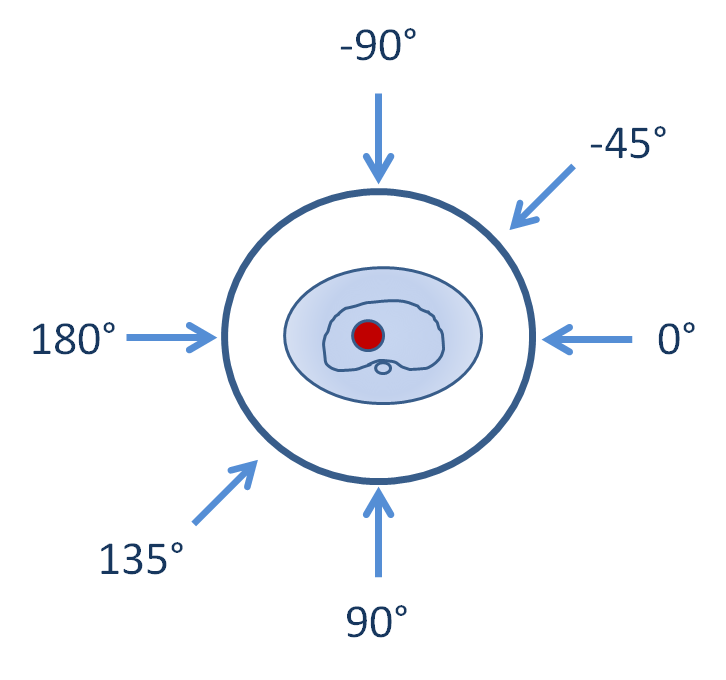
\includegraphics[scale=0.4]{GantryDirection.png}
  \caption{Entry channels for different gantry directions for a couch angle of 90$^{\circ}$.}
  \label{gantrydirection}
 \end{center}
\end{figure}


\newpage

\subsubsection{Motion trajectories}

As the reconstruction of the 4DCTs was based on the time scale a phase-based motion state detection was employed. A sinus motion was 
chosen for the motion trajectories. In order to consider possible divergence in the heartbeat motion pattern of patients, 
different periods (1 s and 0.7 s) as well as different starting phases (0$^{\circ}$ and 90$^{\circ}$) were used. 


\subsubsection{Margins}

Besides the original volume of the CTV safety margins have been added to the volumes of the treatment planning study. These margins were applied 
in order to account for theoretically possible deviations in between treatment planning and delivery, like slight positioning errors, changes 
between CT acquisition and treatment delivery etc. Isotropic safety margins of 3mm, 5mm and 7mm have been chosen. The ITV volumes used as the 
final target were generated from the original CTV contour as well as the CTVs with margin, so that potential range variations were considered 
in the margins. 
% By studying the dose to OAR when depositing dose in the so increased target, possible limitations on the needed accuracy were analyzed. 


\subsection{Treatment planning studies}

3D treatment plans were produced on one hand as reference values to the 4D cases, as it represents the ideal but not deliverable dose 
distribution. On the other hand they were also generated in order to study the best suited combinations of beam entry channels 
as well as to study possible safety margin limitations. In order to find a suitable field number and beam direction for the treatment planning 
studies, static simulations on the original CTV volume (LPV together with RPV) with the above mentioned treatment planning parameters were 
carried out for all five patients. 17 different beam channel combinations were studied (see table \ref{tab:fields}). As a criteria for the 
best possible solution the dose to OAR were assessed. Furthermore, different ITV margins (original, an increased with 3mm, 5mm and 7mm margin) 
were studied in 3D treatment plans for all patients. The resulting dose depositions were compared to IMPT dose deliveries (where the esophagus 
was included in the optimization process). Possible limitations were again analyzed according to the dose deposition in the OARs. In order to 
prepare for the 4D simulations, the motion of the PVs due to heartbeat was than assessed. 
4D plans were distinguished between an underlying motion without any compensation, resulting in interplay patterns, and with the application of 
rescanning as motion mitigation technique. For rescanning different rescan numbers (5, 10, 15 and 20) were compared.
Static, interplay as well as rescanning treatment plans for all patients where carried out with one beam channel combination, all four safety 
margins, the stated treatment planning parameters and the four stated motion trajectories. 


\subsection{Analysis}

Both the dose deposition in OAR as well as dose homogeneity in the target volume were studied. For the OAR dose-volume restriction in 
esophagus, trachea, aorta and the whole heart were compared to values from RTOG study protocols (see next paragraph). 
As further OAR cardiac substructures (ventricles and coronary arteries) were studied. Here the mean dose into the structures as well as the 
maximum point dose and the maximal irradiated volume (thus sum over all voxels of the organ which receive dose) were analyzed. In general, the 
median values of these parameters over all patients were further calculated. Besides the second quartile (median, 50th percentile) also the 
third quartile (75th percentile) was assessed. For comparison of the resulting dose coverage in the target region dose-volume-histograms 
(DVHs) were studied. Furthermore motion-volume-histograms (MVHs) \cite{Ric13} were generated displaying the relative displacement of every 
voxel of the investigated volume to the reference phase in all three motion directions. With these the resulting motion of the PV due to 
heartbeat could be assessed. 

\subsubsection{Dose-volume constraints for organs at risk}

The dose deposition in the OAR is an important limitation and selection criteria when studying the field number and beam channel 
direction as well as the possible safety margin limitations. Since a single fraction of 25 Gy or higher is assumed to be used in the 
presented, non-invasive treatment modality, dose tolerance limits used in stereotactic body radiotherapy (SBRT) are highly related. An 
extensive collection of dose-volume-limits for SBRT are presented in Grimm et al. \cite{Gri11} and the AAPM Task Group Report \cite{AAPM10}.  
Both are literature reviews of limits utilized and reported in existing publications. For the OAR in the here presented 
treatment planning study (esophagus, trachea, heart and aorta) the dose-volume-limits in both literature reviews were taken from the 
Radiation Therapy Oncology Group (RTOG). The RTOG is a national clinical cooperative group of over 360 institutions across the United 
States and Canada, which was funded by the National Cancer Institute (NCI) \cite{RTOG}. In their study protocols RTOG 0631 
(a phase II/III trial of SBRT for localized spine metastasis) \cite{RTOG0631} and RTOG 0915 (a randomized phase II trial of SBRT for 
medically inoperable patients with stage I peripheral non-small cell lunger cancer) \cite{RTOG0915} the following dose-volume-limits 
were stated (see table \ref{tab:RTOG}). 

\vspace*{-0.8cm}

\begin{table}[H]
  \centering
  \caption{Dose-volume limits for OAR.}
  \begin{tabular}{|c|c|c|c|}
    \hline\hline
    OAR & Volume [cc] & Dose [Gy] & endpoint \\
    \hline
    Aorta / great vessels & 10 & 31 & Aneurysm \\
    Esophagus & 5 & 11.9 &  Stenosis / fistula \\
    Heart & 15 & 16 & Pericarditis \\
    Trachea & 4 & 10.5 & Stenosis / fistula \\
    \hline\hline
  \end{tabular}
  \label{tab:RTOG}
\end{table}

% %%%%%%%%%%%%%%%%%%%%%%%%%%%%%%%%%%
% RTOG 0915 zitat:
% absolute limits, and treatment delivery that exceeds these limits will constitute a protocol violation (See Section 6.7). The dose is listed 
% as total delivered. These limits were formulated with the approval of the study committee (Principal Investigators and Co-Chairs) using 
% tolerance data, historical data as listed in section 1 with special weighting to the RTOG experience (in reference to the 34 Gy dose) and that 
% of Chang, et al. from MD Anderson (in reference to the 12 Gy times 4 fractions arm).
% 
% in RTOG heart critical structure! here target
% %%%%%%%%%%%%%%%%%%%%%%%%%%%%%%%%%%

% \vspace*{-0.8cm}

Since the heart is not only a critical organ but also the target site in this treatment modality, further differentiation of 
limits depending on the substructures of the heart are needed. Unfortunately, data herefore is scarce and 
literature on cardiac disease resulting from radiation exposure mostly reliant on patient data treated with cancer radiotherapy 
(in particular breast cancer and Hodgkin's lymphoma) or atomic bomb survivors. Besides 
the stated dose-volume limitation, the mean dose and maximum point dose to the whole heart was studied. 
Furthermore the maximal irradiated heart volume (each voxel which received a dose deposition) was examined. 
Concerning substructures the left and right ventricle as well as the coronary arteries were analyzed 
for mean and maximum dose deposition and maximal irradiated volume contribution. 
% Also the mean and maximum dose as well as maximum volume in the AV node was studied. 
% For the analysis of the dose deposition to the heart it can be concluded that the mean and maximum dose to the 
% whole heart is an important factor, and that furthermore the coronary arteries and the left ventricle are important substructures. 
% These structures were studied according to the mean and maximum received dose. Furthermore the maximum irradiated volume was 
% investigated. XXX

% \newpage

\subsubsection{Dose deposition in target volume and motion of PVs}

The V95 (measure of dose coverage) and V107 (measure 
of over dosage) of the CTVs were analyzed. As an indicator for the dose homogeneity, the width of the dose fall off was determined by analyzing 
the difference D5-D95. The stated values have been evaluated for all beam applications (static, interplay, rescanning). Static thereby means that 
no motion was included, resulting in a 3D case. This is only used as a reference value for the 4D cases interplay and rescanning, as the static 
case represents the ideal, but not deliverable dose distribution. 


\section{Results}

In the following the results of the beam direction and safety margin study, PV motion assessment as well as the treatment planning studies 
will be discussed. As a criteria for an adequate field number and beam channel direction as well as safety margin limitation the dose to OAR 
will be presented in detail. 
% Dose-volume results for esophagus, trachea, aorta and the whole heart are shown. Furthermore dose deposition in 
% critical substructures of the heart (left ventricle (LV), right venticle (RV), left coronary arteries 
% (LCA) and right coronary arteries (RCA)) are presented. 
The motion is shown as the relative displacement to the reference motion phase. 
For the treatment planning study different dose analysis parameters will be presented and compared for different cases (static, interplay and rescanning). 

\subsection{Beam direction}

% %%%%%%%%%%%%%%%%%%%%%%%%%%
% - difference for fixed beam direction in between patients small!
% - difference for patient in between beam directions rather small!
% - more robust to have bigger angle in between fields -> if something displaced (e.g. eso) than not more than one field affected
% %%%%%%%%%%%%%%%%%%%%%%%%%

In figure \ref{beamdirection} the resulting dose to the pertinent OARs is shown for all studied beam directions and patients. 
The corresponding volumes result from the dose volume limits (e.g. 5 cm$^{3}$ for esophagus, see table 
\ref{tab:RTOG}). The stated, recommended dose limit is represented by a dashed line in the plots. In all studied cases, the 
difference between different beam directions for a certain patient is rather small, resulting in no obvious preferable beam direction for 
the five studied patient. For the four studied OAR it becomes furthermore obvious, that while some organs, like trachea and aorta, are well 
spared for almost all beam directions in all patients, esophagus and in particular the heart are much more critical.

\newpage

%%%%%%%%%%%%%%%%%%%%%%%%%
%%%%%%%% DOSE TO OAR
%%%%%%%%%%%%%%%%%%%%%%%%%

% \newpage

\begin{figure}[H]
\subfigure[Esophagus]{
 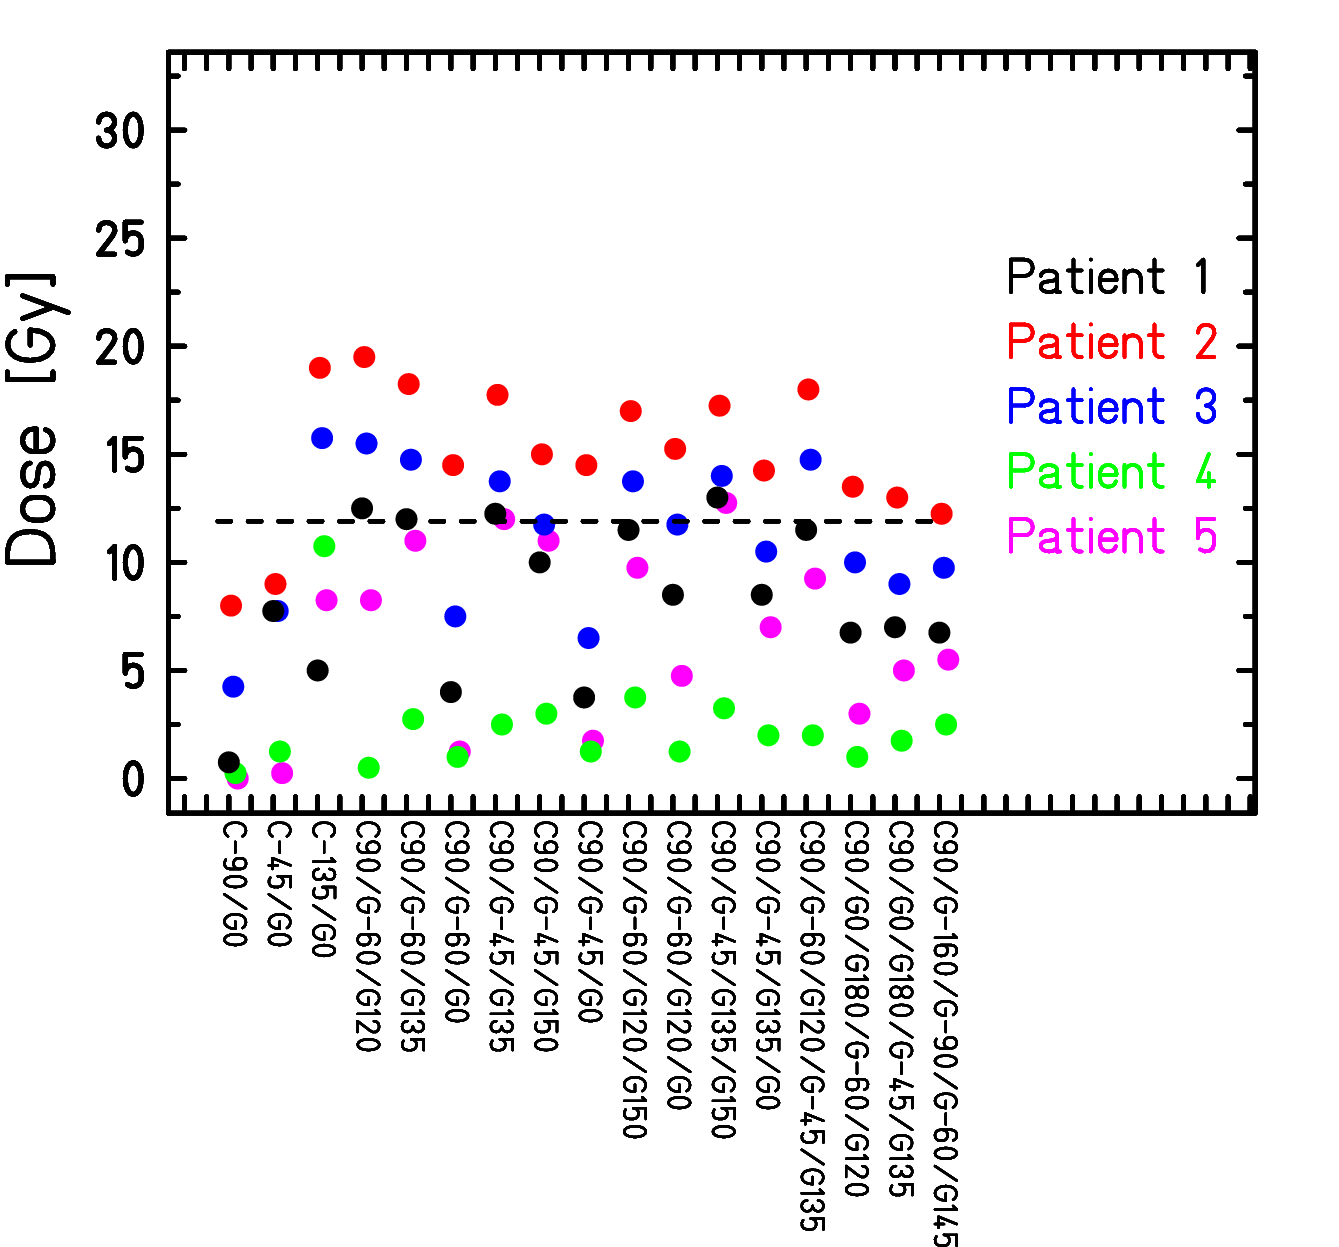
\includegraphics[scale=0.18]{Mayo_Human_BeamDirection_ESO.png}
 }
 \subfigure[Trachea]{
 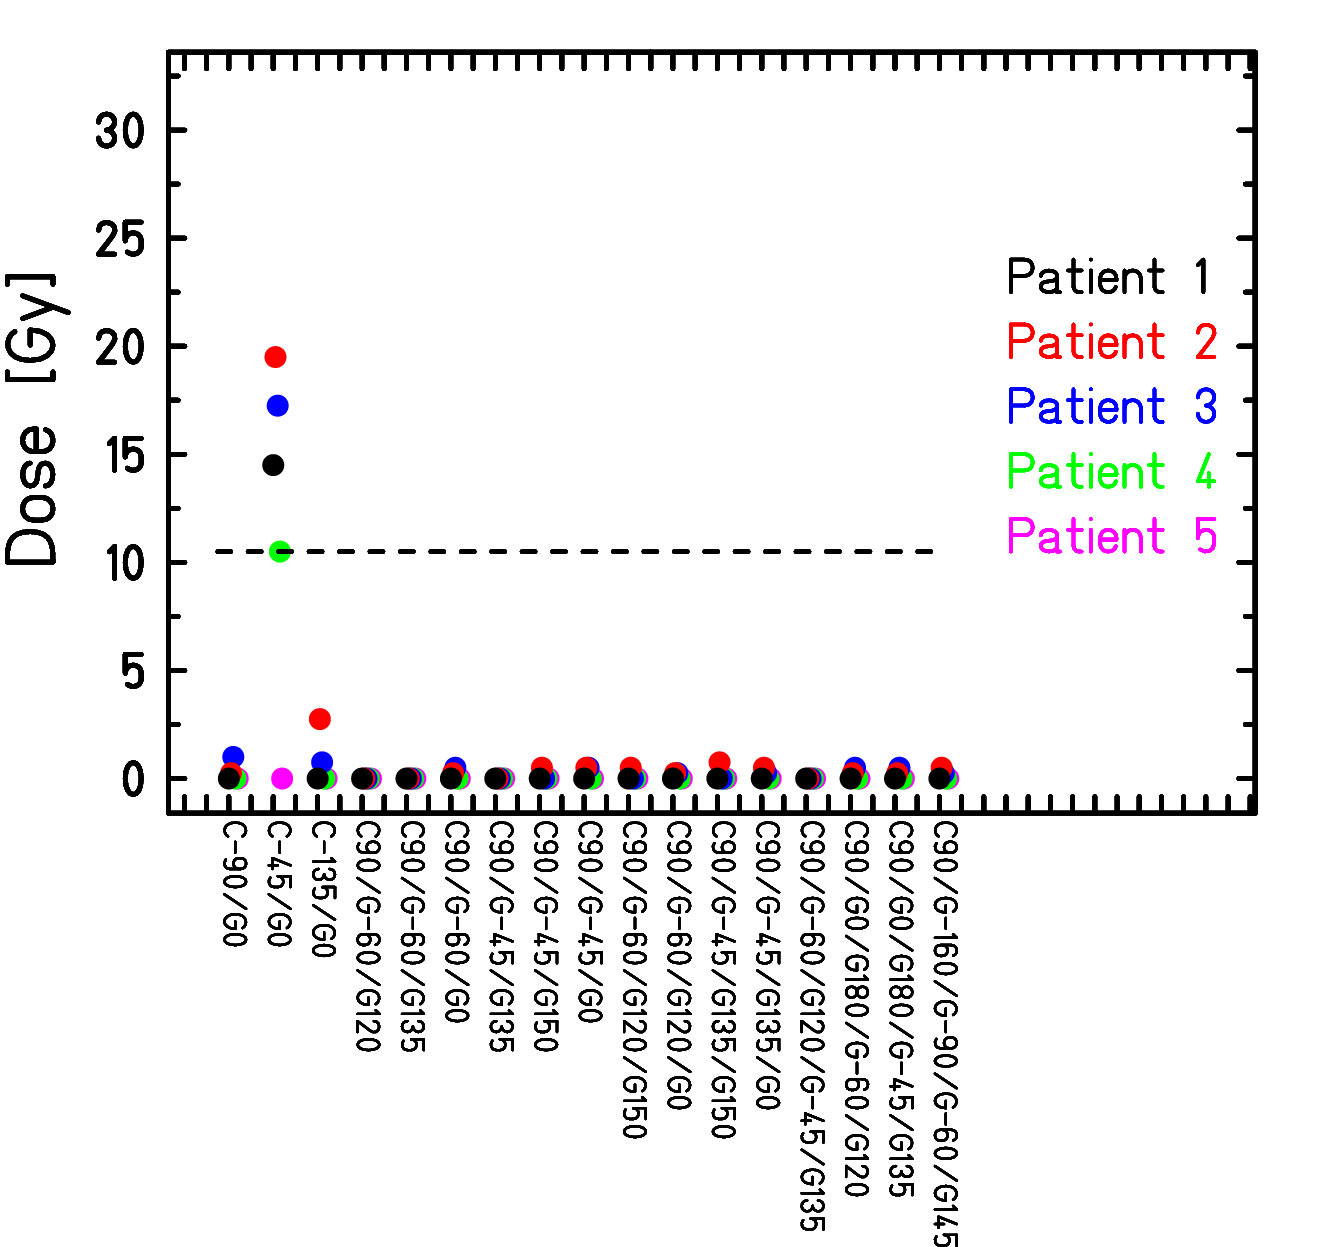
\includegraphics[scale=0.18]{Mayo_Human_BeamDirection_TRACHEA.png}
 }
  \subfigure[Heart]{
 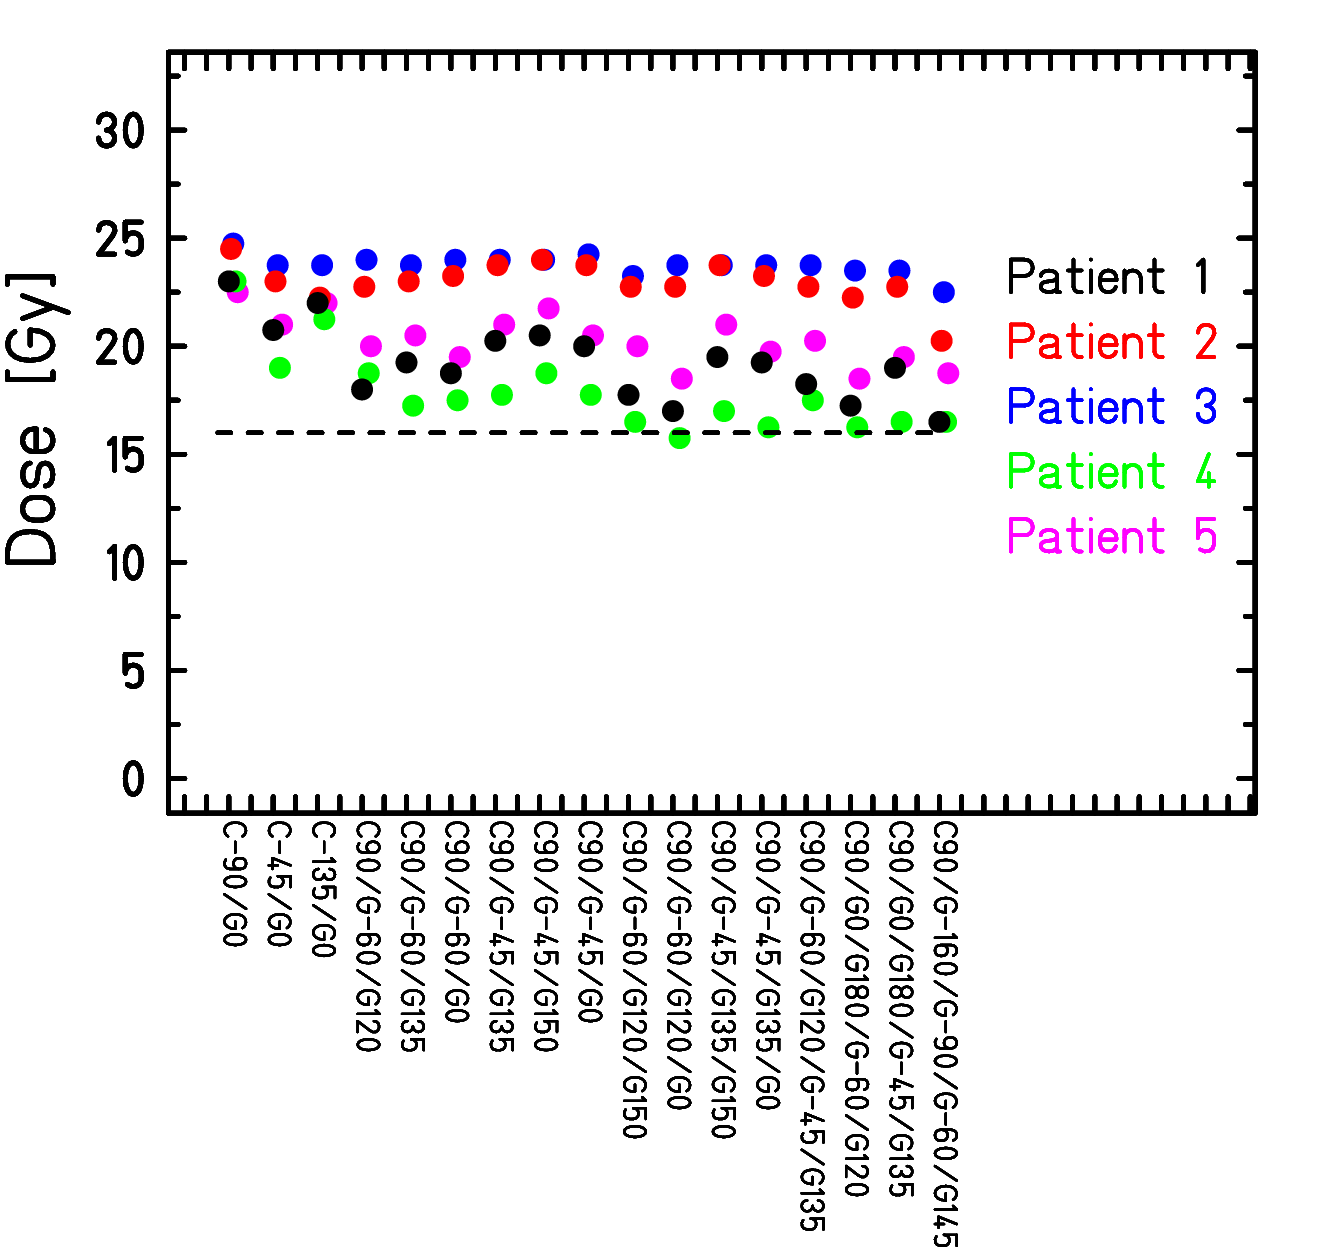
\includegraphics[scale=0.18]{Mayo_Human_BeamDirection_HEARTwoOverlap.png}
 }
  \subfigure[Aorta]{
 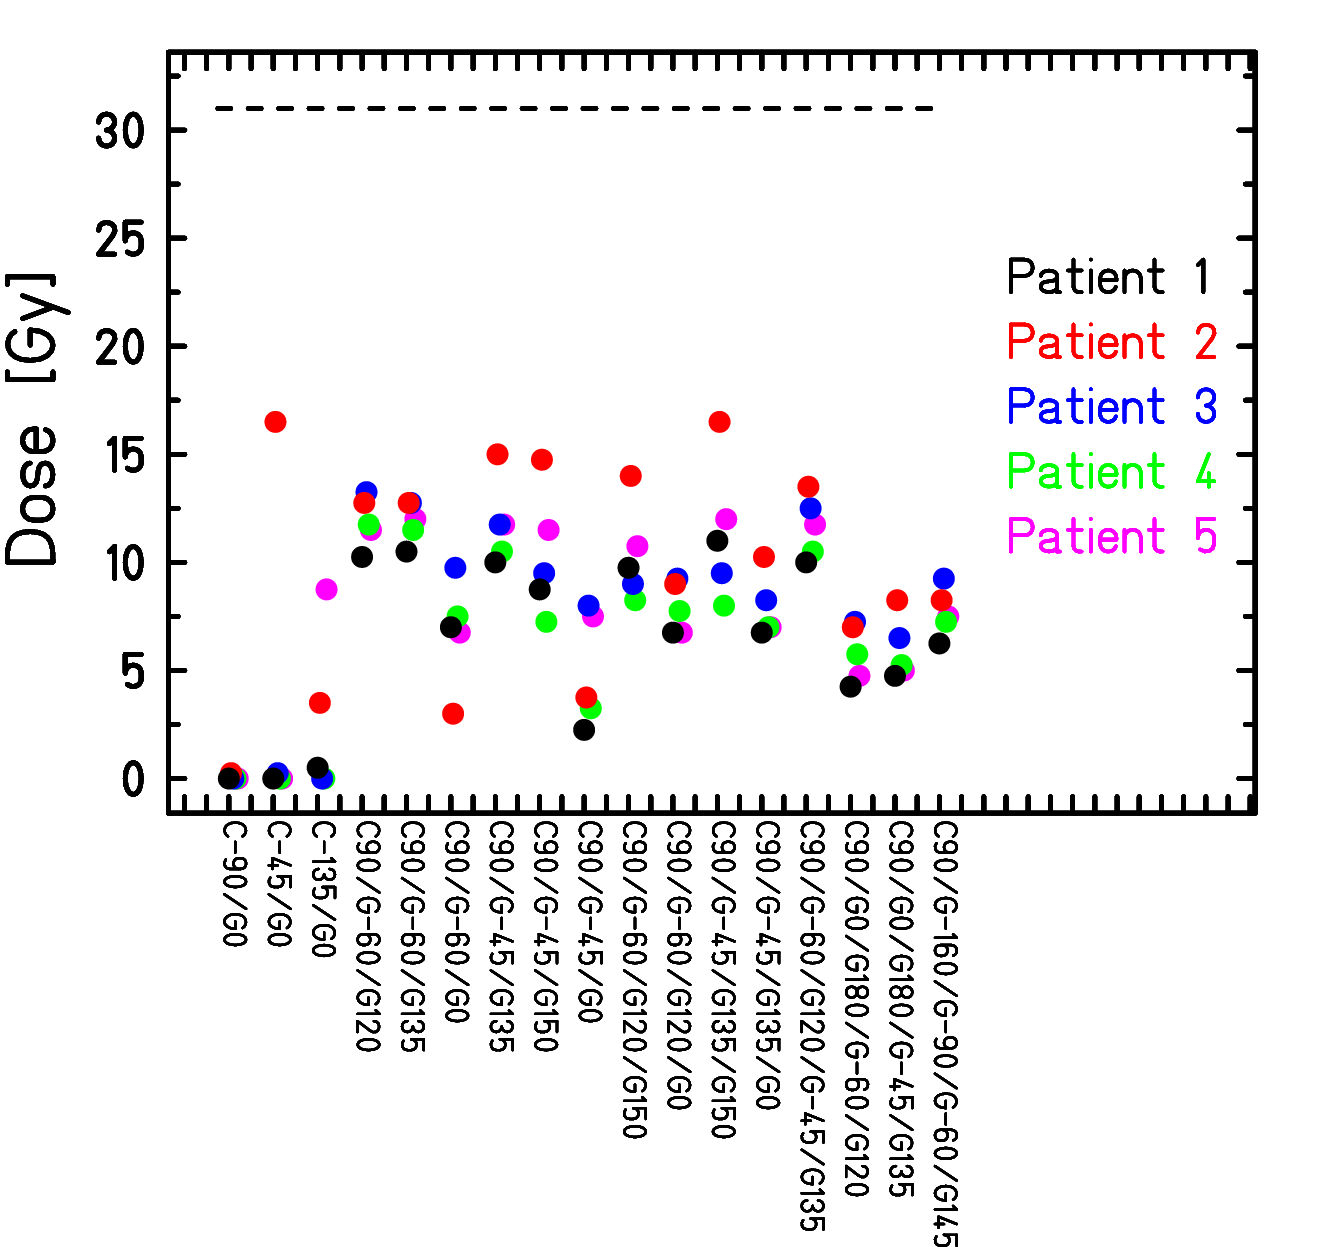
\includegraphics[scale=0.18]{Mayo_Human_BeamDirection_AORTA.png}
 }
%  \subfigure[Left coronary artery]{
%  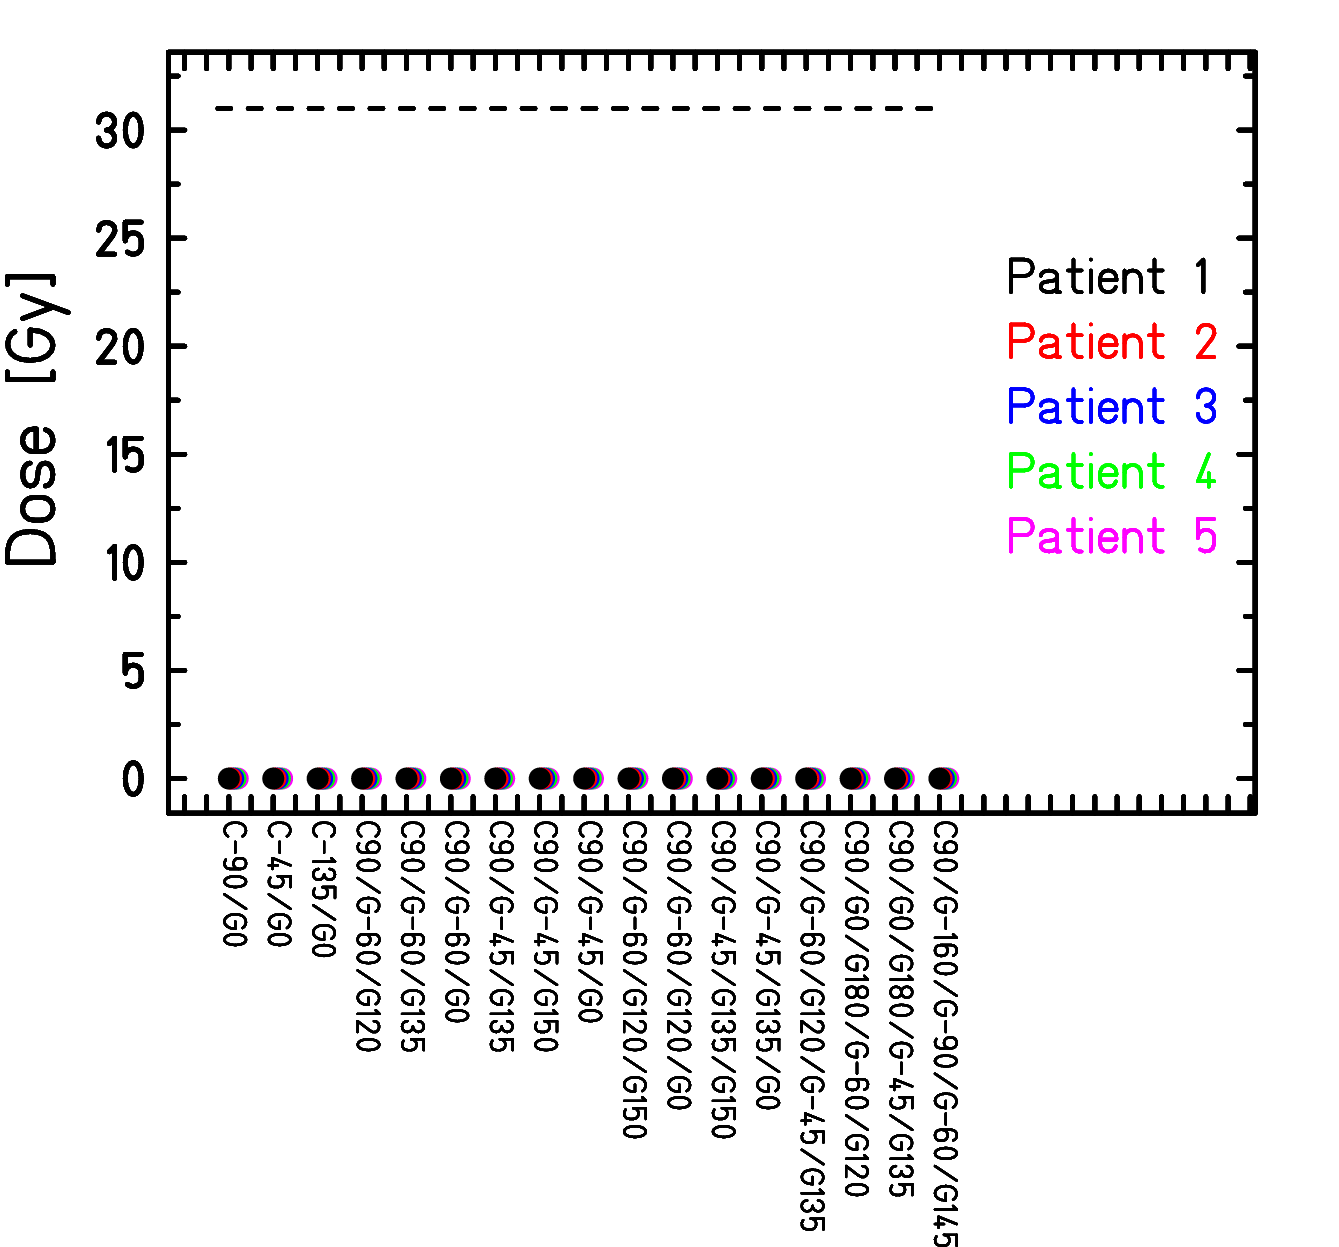
\includegraphics[scale=0.14]{Mayo_Human_BeamDirection_LCA.png}
%  }
%  \subfigure[Right coronary artery]{
%  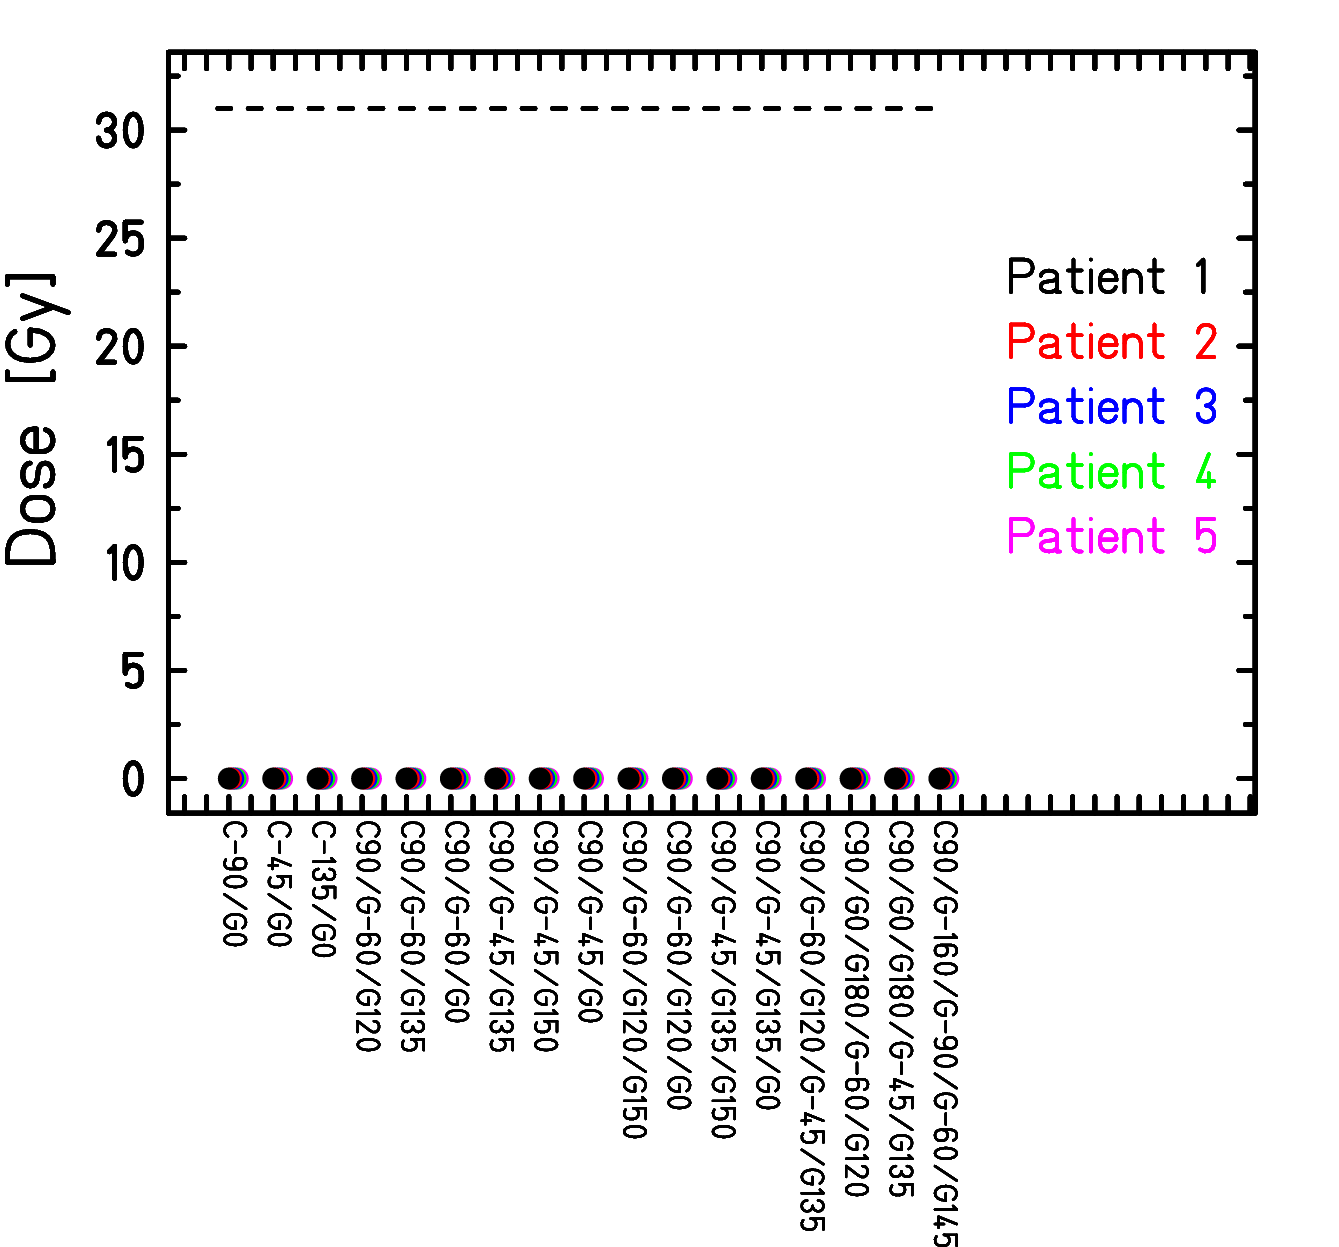
\includegraphics[scale=0.14]{Mayo_Human_BeamDirection_RCA.png}
%  }
\caption{Dose-volume data of different OAR when irradiating the LPV and RPV as SFUD in the five patient data sets with different field numbers 
(1 field, 2 fields, 3 fields, 4 fields) and different beam directions. The dose-volume-limit for each critical organ is indicated with a dashed line in 
each plot, respectively.}
\label{beamdirection}
\end{figure}

% In the esophagus the average dose over all patients is (6.53 $\pm$ 5.55) Gy for one field, (9.08 $\pm$ 5.69) Gy for two fields, 
% (9.91 $\pm$ 4.92) Gy for three fields and (9.11 $\pm$ 5.36) Gy for four fields. The relatively high standard deviations show that the result 
% is very dependent on the underlying patient anatomy. 
In the esophagus the median dose over all patients is  7.8Gy (75th percentile: 9.0Gy) for one field, 10.5Gy (13.9Gy) for 
two fields, 11.0Gy (13.9Gy) for three fields and 9.1Gy (12.8Gy) for four fields. 
The result is dependent on the underlying patient anatomy. 
While the majority of the beam directions for patient 1, 4 and 5 remain under the 
respective dose-volume limit, patient 2 and 3 result in many dose-volume exceeding depositions. For these patients a dose deposition 
of 11.9 Gy or less are achieved in only about 2\% and 65\% of studied cases, for patient 2 and 3, respectively. While a single field yields 
very small dose deposition in the esophagus, these beam channels result in higher dose depositions in the heart and cardiac substructures like 
the coronary arteries (see figure \ref{beamdirection_dose_ca}) and are thus inapplicable. For patient 2 higher field numbers and thus more beam 
directions result in dose limit exceeding depositions. Due to this result a different treatment delivery (intensity modulated particle 
therapy, IMPT) was additionally studied in comparison to a simple SFUD irradiation in further dose deposition studies (see section \ref{safetymarginlimitation}).\newline
\newline
The dose volume limit for the heart is exceeded in all patients for all beam directions. As the heart is not only an 
OAR in this treatment modality, but some of its substructure are also the target itself, a closer analysis of the dose deposition in the heart 
is required. In figure \ref{beamdirection_dose_heart} the mean and maximal dose deposition in the whole heart as well as the maximal 
irradiated volume are shown. The mean dose over all patients 
and beam directions is found to have a median of 1.3Gy (75th percentile: 1.5Gy). 
% (1.30 $\pm$ 4.14)Gy. 
% The maximum point dose is found to (26.74 $\pm$ 0.78)Gy. 
The median over the maximum point dose is found to 26.6Gy (27.1Gy).
Concerning the maximal irradiated volume it can be seen that expect of one result less than 30\% of the heart is irradiated in all other cases. 
In the case of couch position 90$^{\circ}$ and gantry angles of -160$^{\circ}$, -90$^{\circ}$, -60$^{\circ}$ and 145$^{\circ}$ these maximal 
volume is drastically increased, and reaches up to 49.9\% for patient 2. Hence this beam channel case (beam channel case 17) will be 
stated separately in the following analysis. 
% The overall mean irradiated volume results to (16.63 $\pm$ 4.92)\%, excluding the case of couch position 90$^{\circ}$ and gantry angles of -160$^{\circ}$, 
% -90$^{\circ}$, -60$^{\circ}$ and 145$^{\circ}$, and to (18.11 $\pm$ 7.69)\% including this case.\newline
The median of the maximal irradiated volume over all patients results to 17.4\% (20.8\%), excluding beam channel case 17 
and to 16.8\% (20.5\%) including this case.\newline
\newline
For results for the dose deposition in the cardiac substructures are presented in figure \ref{beamdirection_dose_ventricle} - 
figure \ref{beamdirection_volume_ca}. For the ventricles, the mean dose to both LV and RV is negligible. 
% rather small for all patients and beam directions, resulting in a median deposition of 0.01Gy (75th percentile: 0.12Gy) for LV and 0Gy (75th percentile: 0.14Gy) 
% for RV. 
% up to 0.50 Gy and 0.25 Gy, for LV and RV, respectively.  
% (0.14 $\pm$ 0.36)Gy and (0.09 $\pm$ 0.16)Gy, for LV and RV, respectively. 
The maximal point dose on the other hand varies dependent on beam direction and patient. Single beam directions yield a high maximal dose 
deposition in the LV as in the case of a couch angle of -90$^{\circ}$ or -135$^{\circ}$ the beam traverses the LV. 
Thus for these beam directions the maximal dose to the RV is smaller. The overall maximal dose deposition results to a median of 
1.4Gy (75th percentile: 7.4Gy) for LV and 1.3Gy (5.0Gy) for RV. 
% up to 10.68 Gy and 6.10 Gy, for LV and RV, respectively. 
%  (4.69 $\pm$ 5.99)Gy and (2.89 $\pm$ 3.21)Gy, for LV and RV, respectively. 
Besides the single beam direction no maximal point dose exceeds 11.2Gy in case of LV and in case of RV all maximal point doses are smaller 
than 10.1Gy. Concerning the maximal irradiated volume of the ventricles, it can be stated that the results differ depending on the studied 
patient. In case of the LV patient 2 has a higher irradiated volume compared to the other patients, while for this patient on the contrary 
the RV is better spared than in other patients. Over all patients the LV is irradiated to a higher extend than the RV. The maximal 
irradiated volume over all beam directions and patients results to a median of 1.2\% (6.0\%) for LV, excluding the case of 
beam channel 17 and to 1.9\% (6.4\%) including this case. For RV it results to 0.2\% (7.6\%) excluding 
the beam channel case and to 0.2\% (8.3\%) including it.
% up to 6.24\% excluding the beam channel case and up to 11.11\% including it. 
% up to 9.17\% in case of LV, excluding the case of a couch angle of -90$^{\circ}$ and gantry angles of -160$^{\circ}$, -90$^{\circ}$, 
% -60$^{\circ}$ and 145$^{\circ}$, and up to 14.32\% including this case. For RV it results 
% up to 6.24\% excluding the beam channel case and up to 11.11\% including it. 
For the coronary arteries the beam channel 17 also results in the highest irradiated volume. 
Even though the coronary arteries are found on the surface of the whole heart and hence also on the ventricles, the irradiated volume of 
these structures differ from the result of the ventricles. Here the RCA are irradiated to a higher extend than the LCA. 
% The mean maximal value for the LCA excluding this case results to (18.33 $\pm$ 15.37)\% and to (20.13 $\pm$ 16.93)\% including it. 
The median maximal value for the LCA results to 15.7\% (28.0\%) including the stated beam channel case 17 and to 15.2\% 
(27.4\%) excluding it. For the RCA the median over the maximal value is much higher and found to 27.9\% (42.4\%) including the beam channel 
case and to 24.8\% (42.1\%) excluding it. 
% The median maximal volume for LCA results to 15.23\% (75th percentile: 27.35\%) excluding the beam channel case and to 15.70\% (75th percentile: 
% 28.03\%) including it. For the RCA the mean maximal value results to (22.41 $\pm$ 19.64)\% and (24.44 $\pm$ 21.40)\%, respectively. 
% The median maximal volume results to 24.81\% (75th percentile: 42.10\%) excluding the case and to 27.86\% (75th percentile: 42.44\%) 
% including it. 
For the mean dose deposited in the LCA one and four beam directions result in an increased dose deposition, while three fields 
yield in general a low mean dose for all studied beam directions and patients. The same is true for the maximum point dose in the LCA. In the 
case of RCA, the result seem to be independent of field number and beam direction. Overall the median over the mean dose results to 0.4Gy 
(1.0Gy) for LCA and 0.6Gy (1.6Gy) for RCA. 
% 2.13 Gy for LCA and 1.89 Gy for RCA. 
% For the maximal point dose the average dose deposition over all beam directions and patients results to (7.64 $\pm$ 6.68)Gy for 
% LCA and (4.81 $\pm$ 4.75)Gy for RCA.\newline
For the maximal point dose the median dose deposition over all beam directions and patients results to 6.8Gy (10.9Gy) for LCA. 
% LCA, including the beam directions and to 6.74Gy (75th percentile: 10.77Gy) excluding it. 
For the RCA it is found to 5.4Gy (7.9Gy). \newline
% including it and 4.93Gy (75th percentile: 7.89Gy) excluding it.\newline
\newline
While it was not expected to find one beam direction feasible for all five patients, it is striking that no beam position results in a clear 
benefit for the OAR of the individual patients. This is due to the challenging position of the PV target site, which is in direct proximity 
to the esophagus and due to the fact that the heart is not only an OAR in this treatment modality, but also the target site itself. 
Nevertheless for the analyzed cardiac substructure, especially the radiosensitive LCA, it can be concluded that three beam channels seem to be 
beneficial for all patients. Regarding the mean dose deposition in the LCA as well as the maximal irradiated heart volume, combined with the 
requirement of a robust treatment and hence the benefit of large gantry angles in between different beam channels, a couch angle of 
-90$^{\circ}$ was chosen together with gantry angles of -45$^{\circ}$, 135$^{\circ}$ and 0$^{\circ}$. These beam channel directions were used 
for a closer analysis of safety margin limitation as well as for the treatment planning studies for all patients. 

\newpage

%%%%%%%%%%%%%%%%%%%%%%%%%
%%%%%%%% DOSE TO THE HEART
%%%%%%%%%%%%%%%%%%%%%%%%%

\vspace*{1cm}

\begin{figure}[H]
\begin{center}
\subfigure[Heart: mean dose]{
 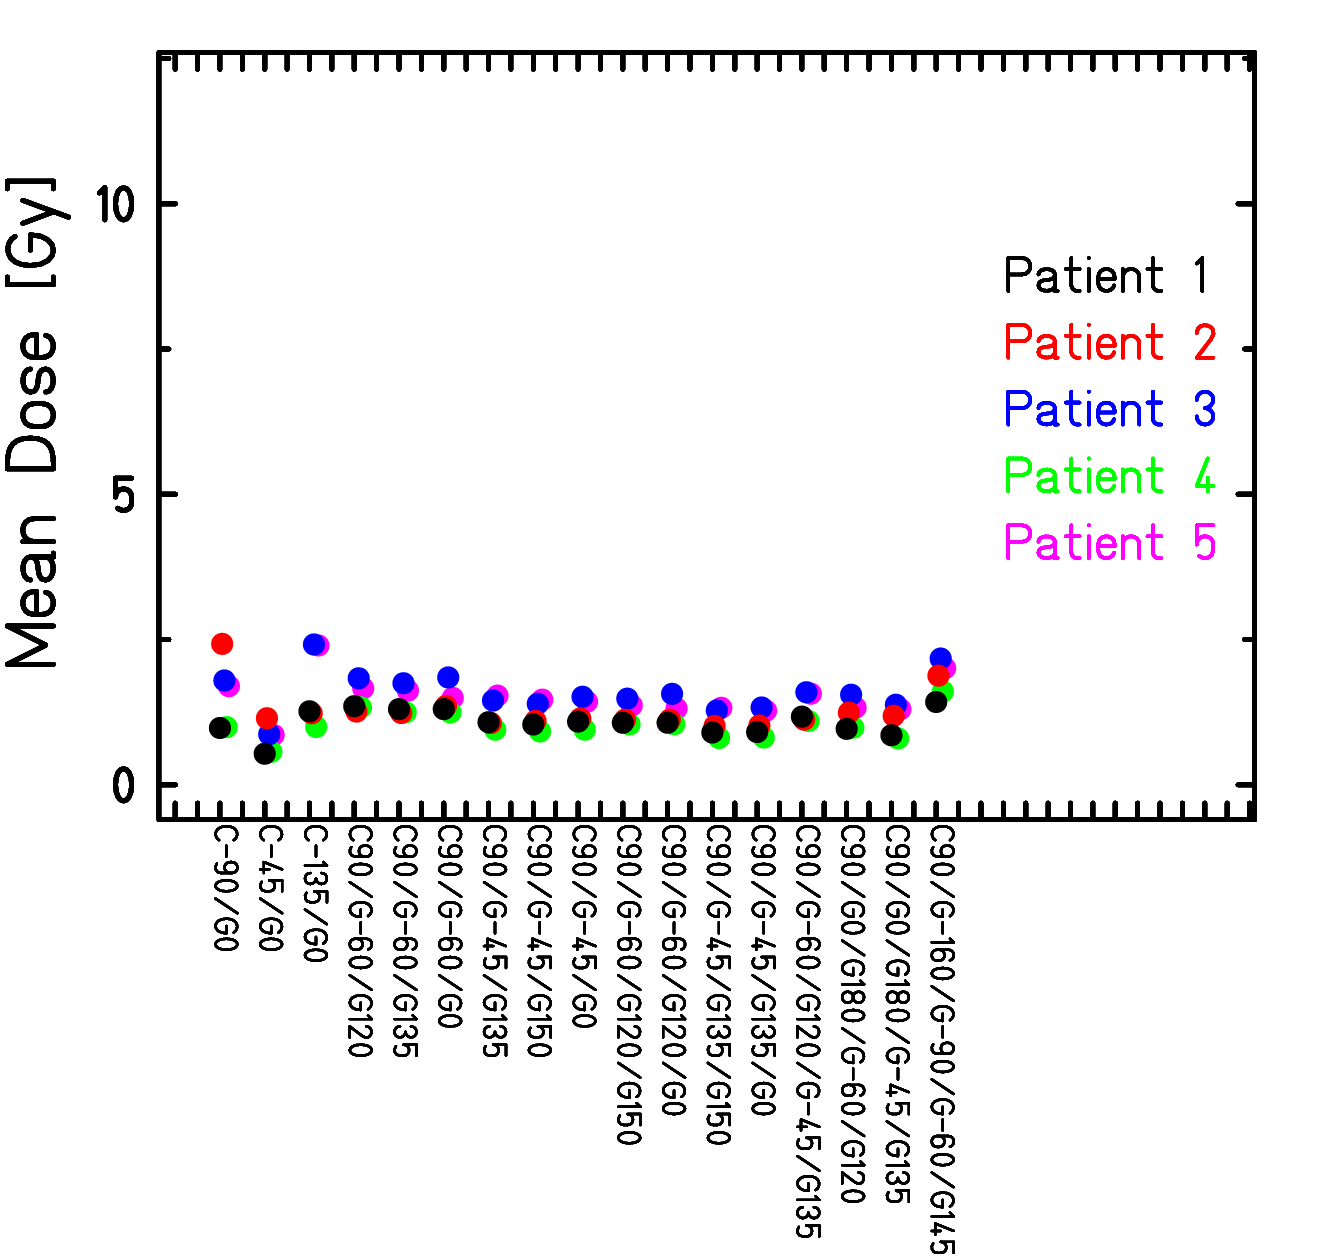
\includegraphics[scale=0.17]{Mayo_Human_BeamDirection_HEARTwoOverlap_MeanDose.png}
 }
 \subfigure[Heart: maximum point dose]{
 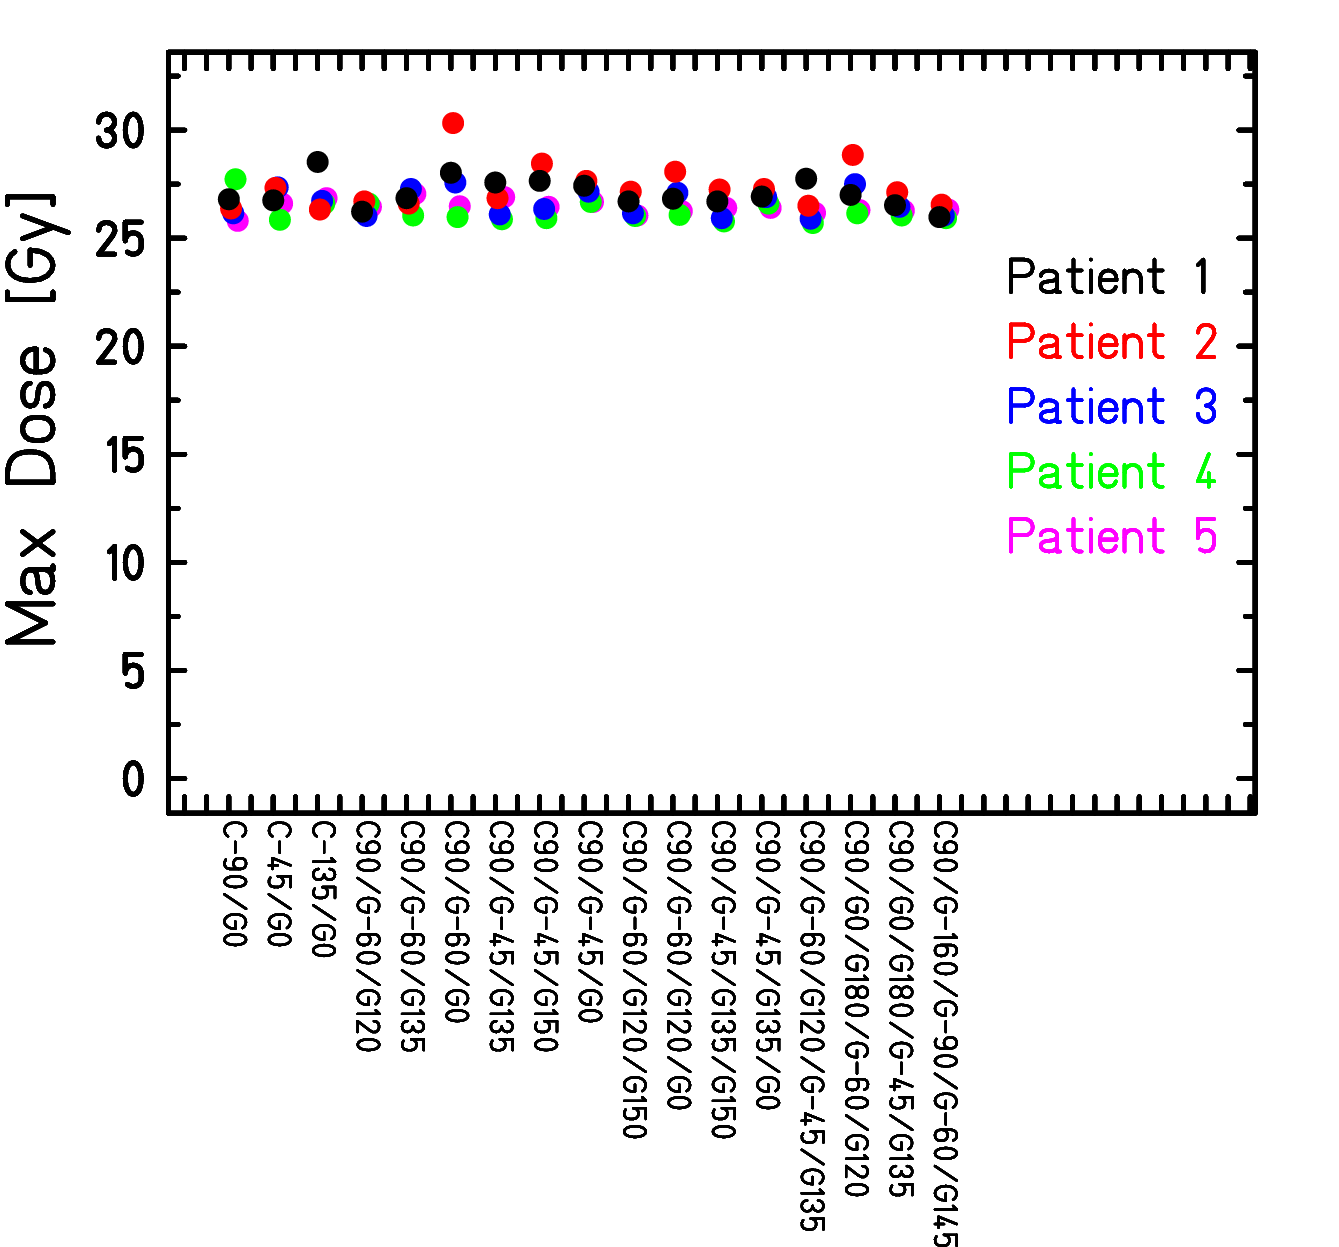
\includegraphics[scale=0.17]{Mayo_Human_BeamDirection_HEARTwoOverlap_MaxDose.png}
 }
 \subfigure[Heart: maximum volume]{
 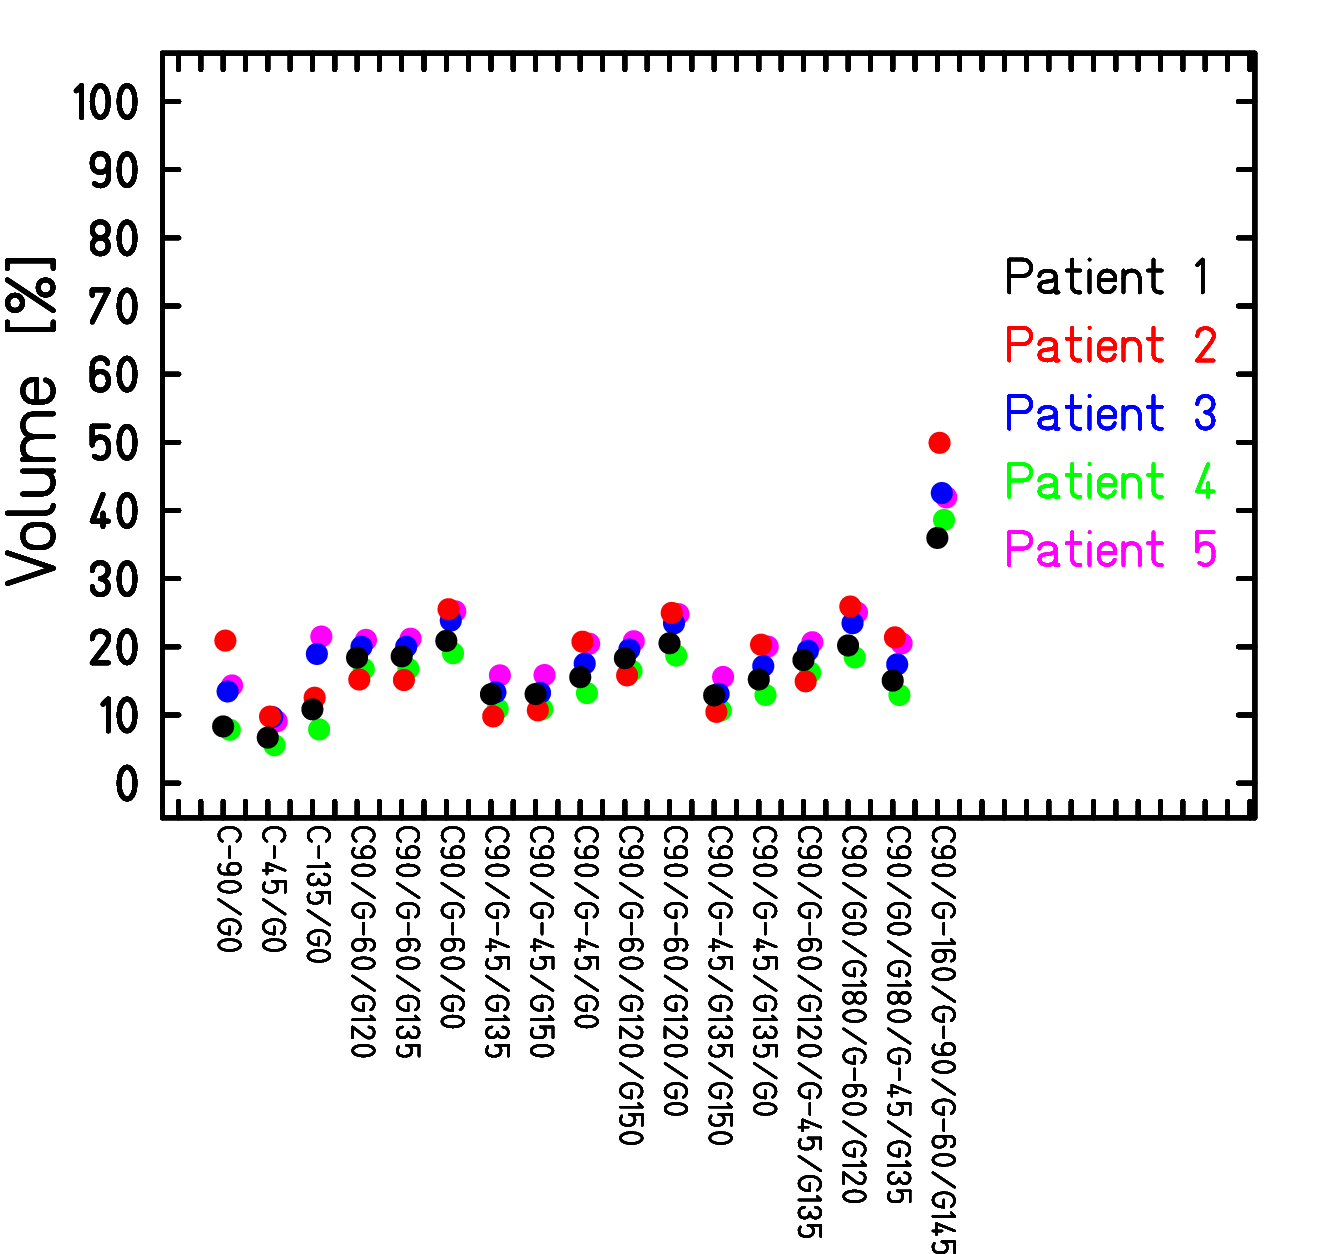
\includegraphics[scale=0.17]{Mayo_Human_BeamDirection_HEARTwoOverlap_MaxVolume.png}
 }
\caption{Mean and maximum dose to the heart and maximal irradiatied heart volume when irradiating the LPV and RPV in the five patient data 
sets with different field numbers and beam directions.}
\label{beamdirection_dose_heart}
\end{center}
\end{figure}

\newpage

\vspace*{1cm}

\begin{figure}[H]
\subfigure[Mean dose: LV]{
 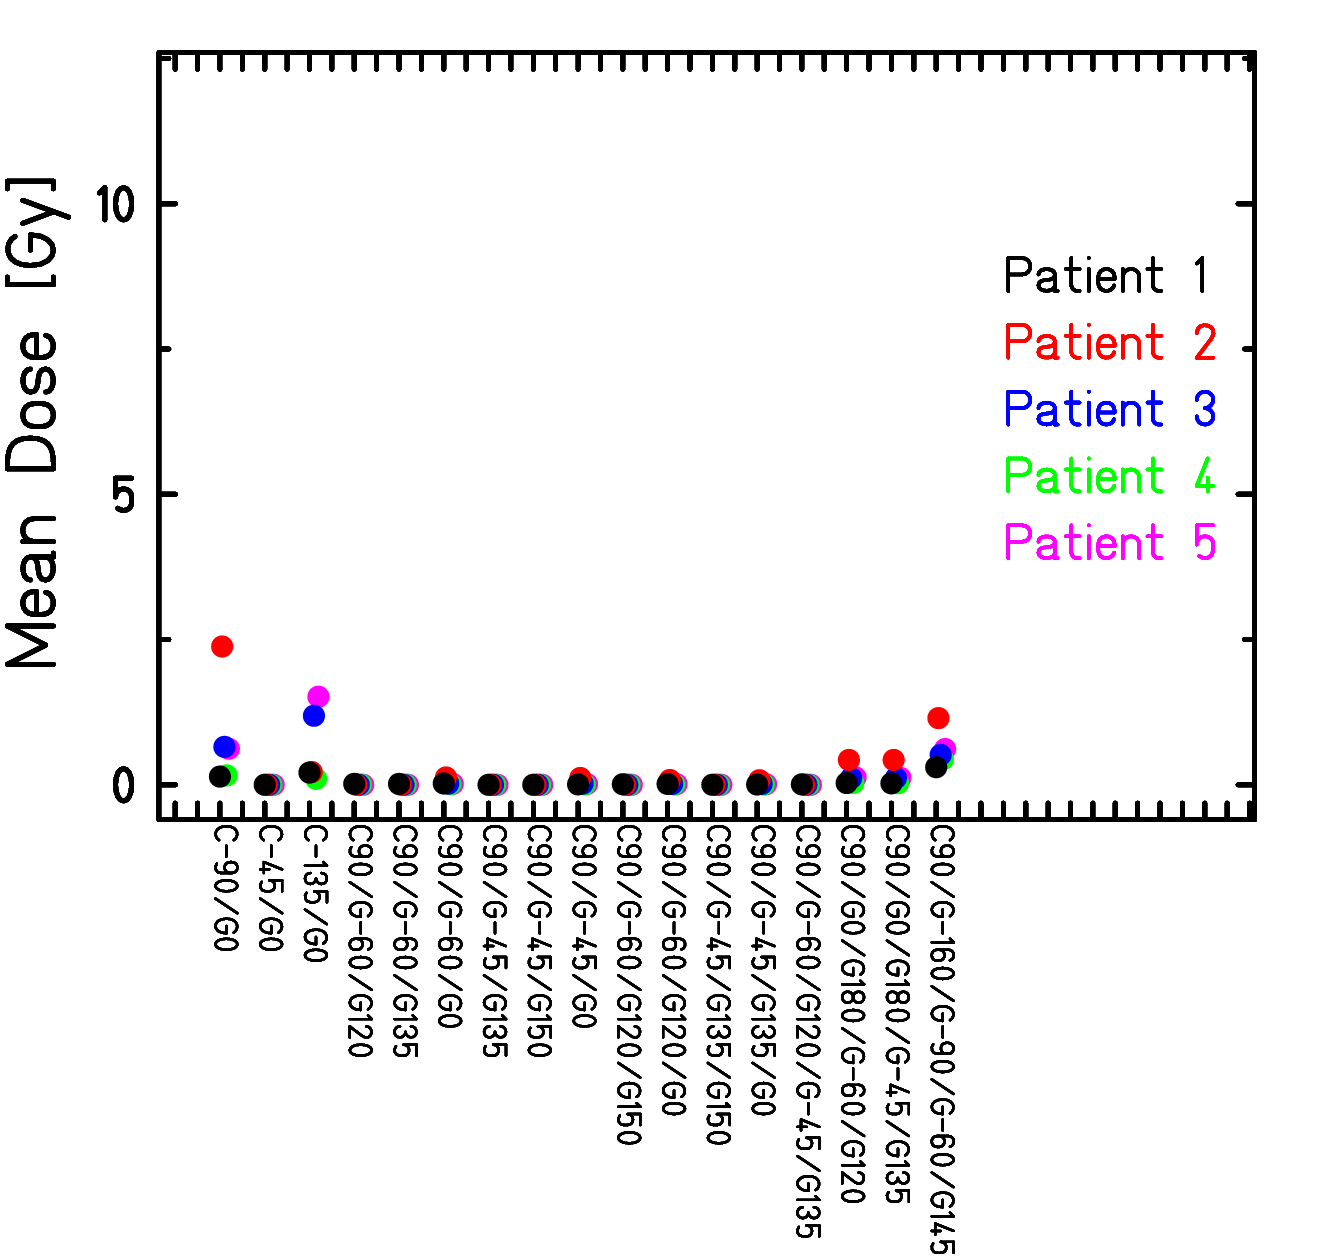
\includegraphics[scale=0.18]{Mayo_Human_BeamDirection_LV_MeanDose.png}
 }
 \subfigure[Mean dose: RV]{
 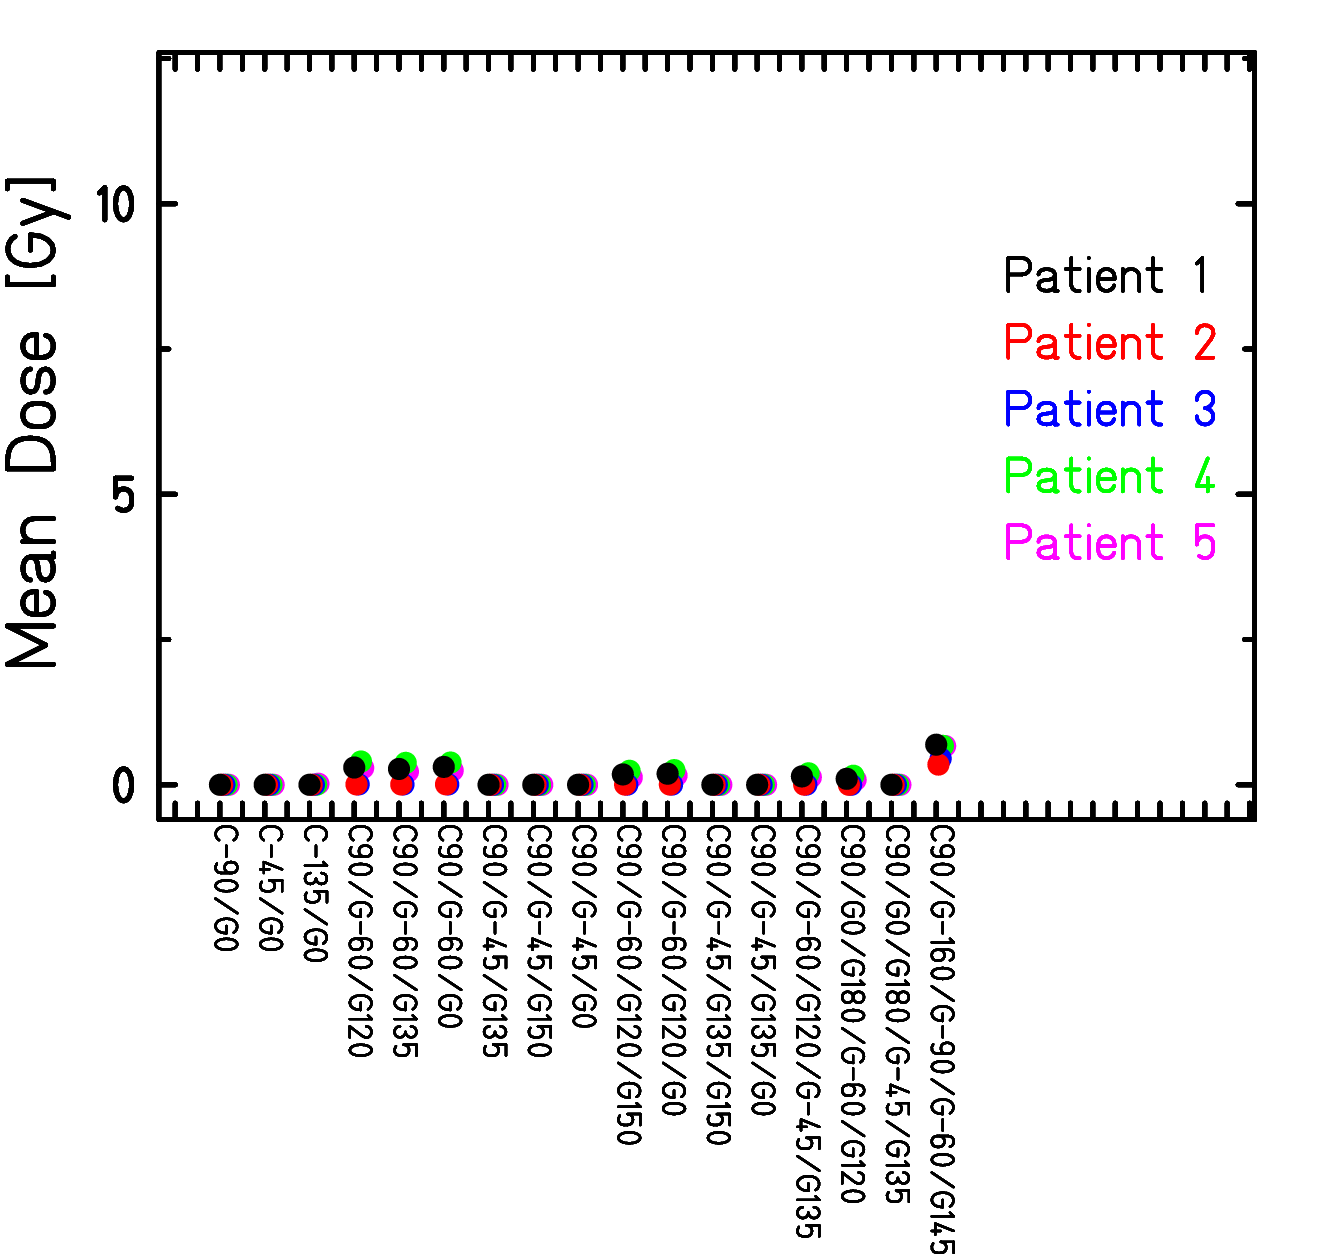
\includegraphics[scale=0.18]{Mayo_Human_BeamDirection_RV_MeanDose.png}
 }
 \subfigure[Maximum point dose: LV]{
 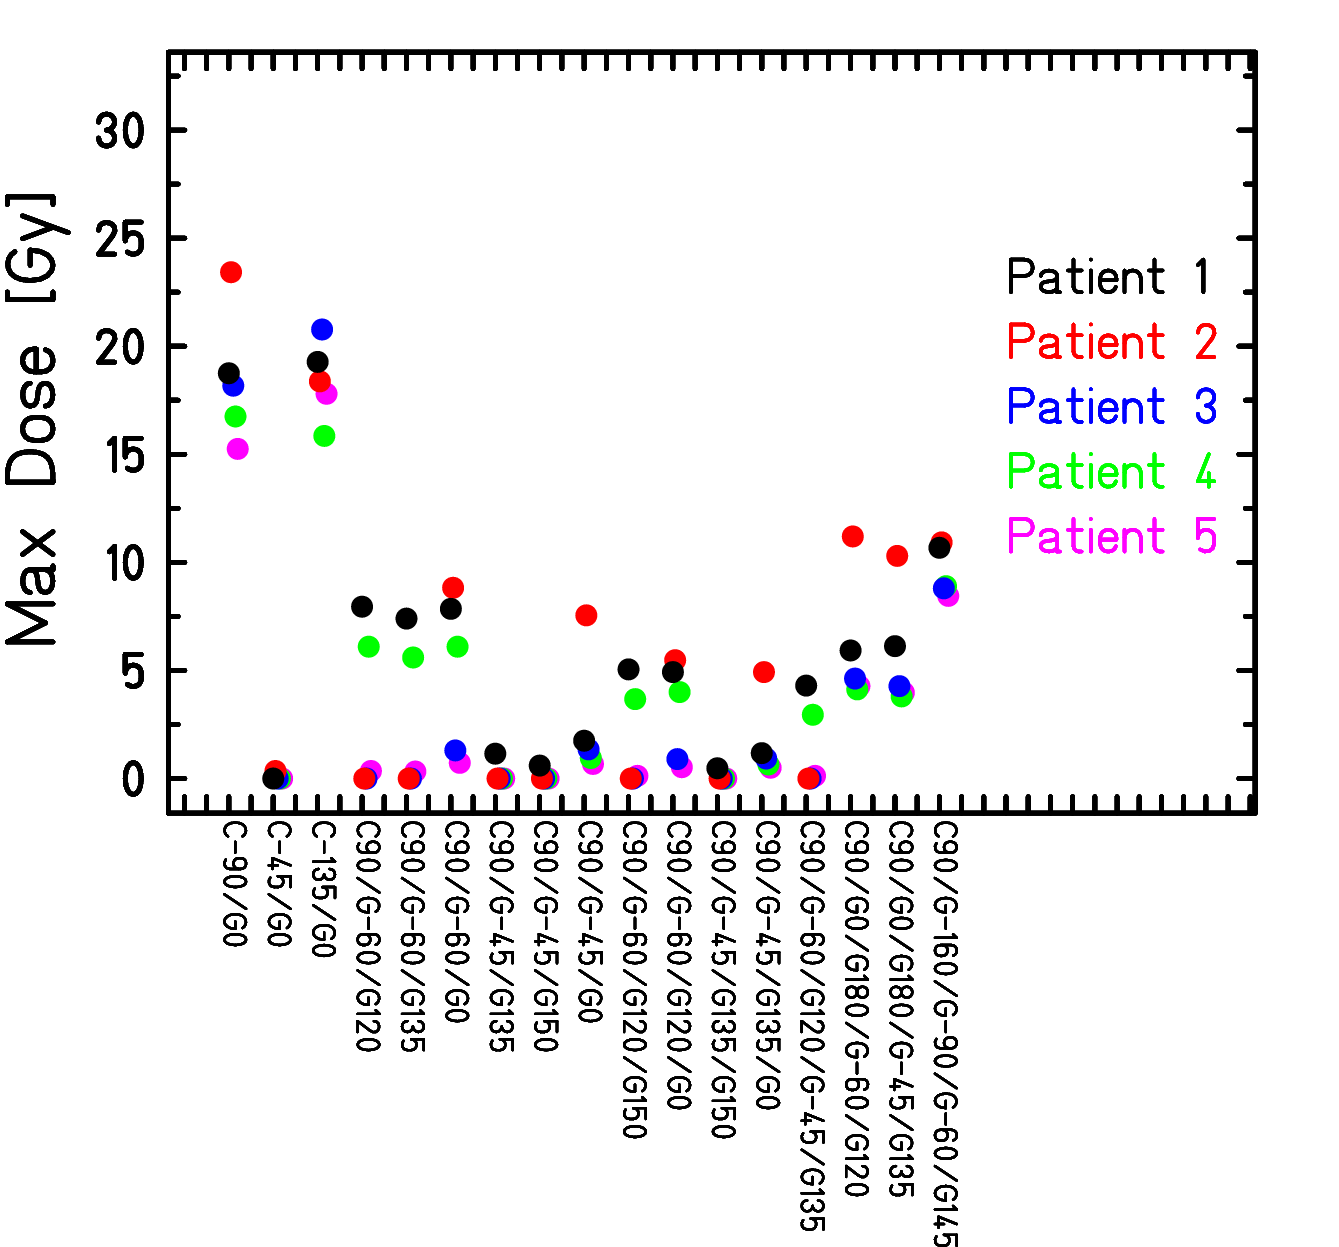
\includegraphics[scale=0.18]{Mayo_Human_BeamDirection_LV_MaxDose.png}
 }
 \subfigure[Maximum point dose: RV]{
 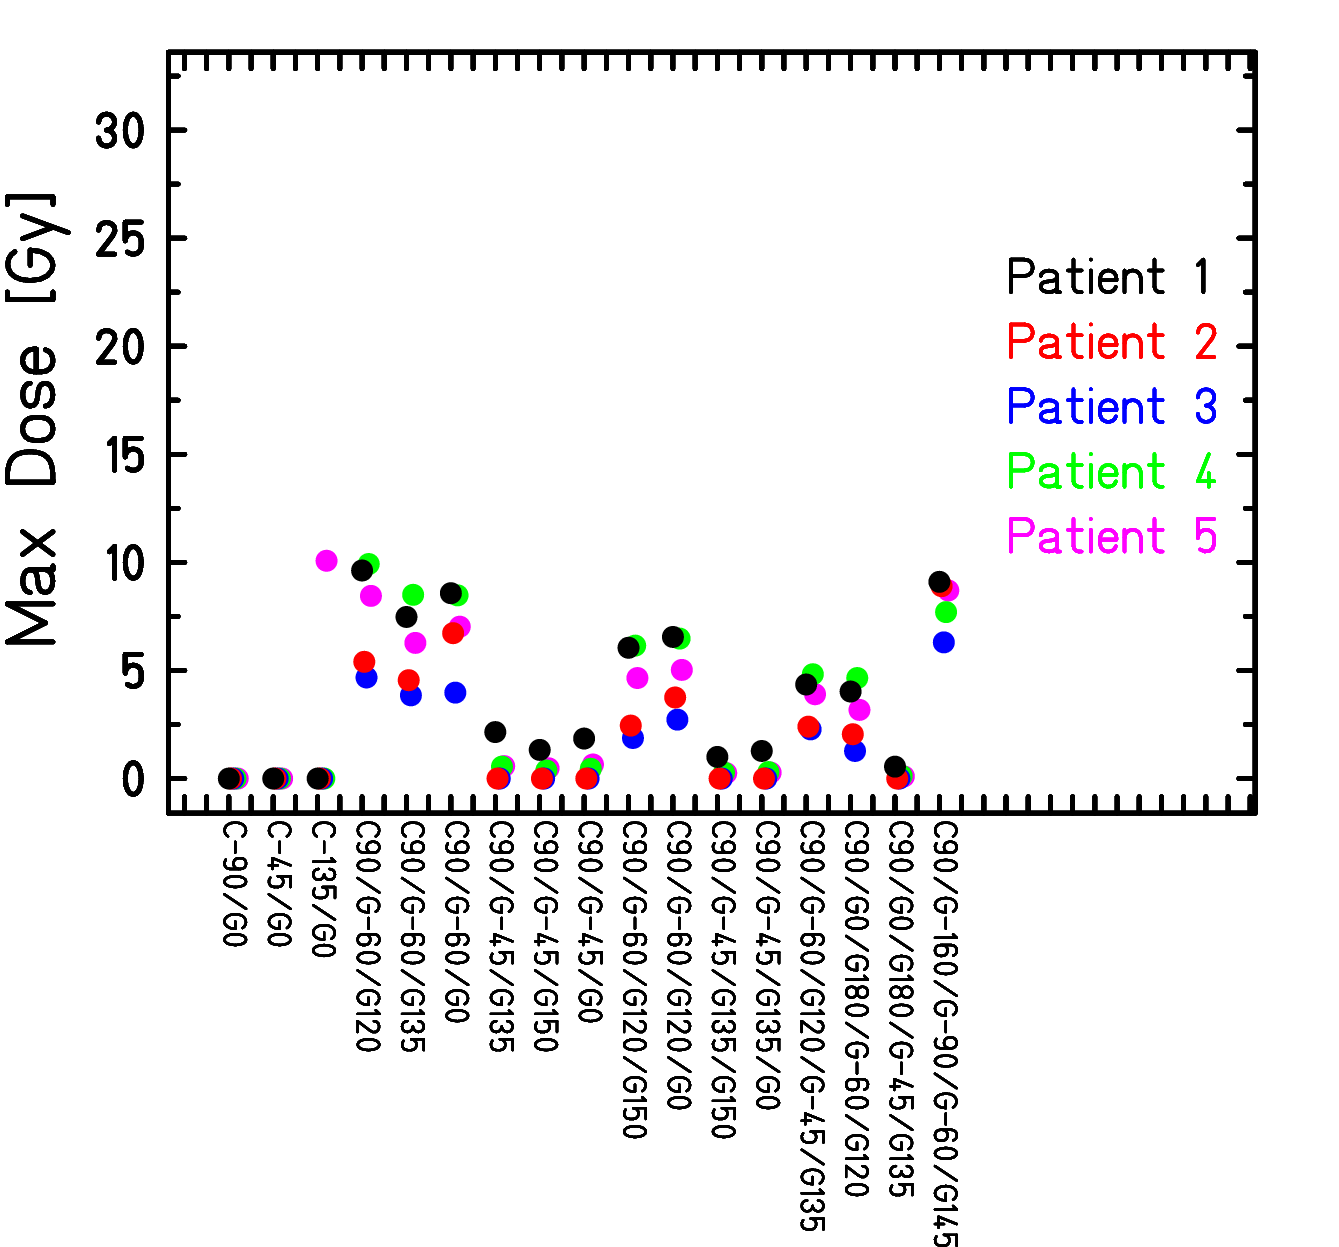
\includegraphics[scale=0.18]{Mayo_Human_BeamDirection_RV_MaxDose.png}
 }
\caption{Mean dose with standard deviation and maximal point dose of left ventricle (LV) and right ventricle (RV), respectively, when 
irradiating the LPV and RPV in the five patient data sets with different field numbers and beam directions.}
\label{beamdirection_dose_ventricle}
\end{figure}

\newpage

\begin{figure}[H]
 \subfigure[Maximum volume: LV]{
 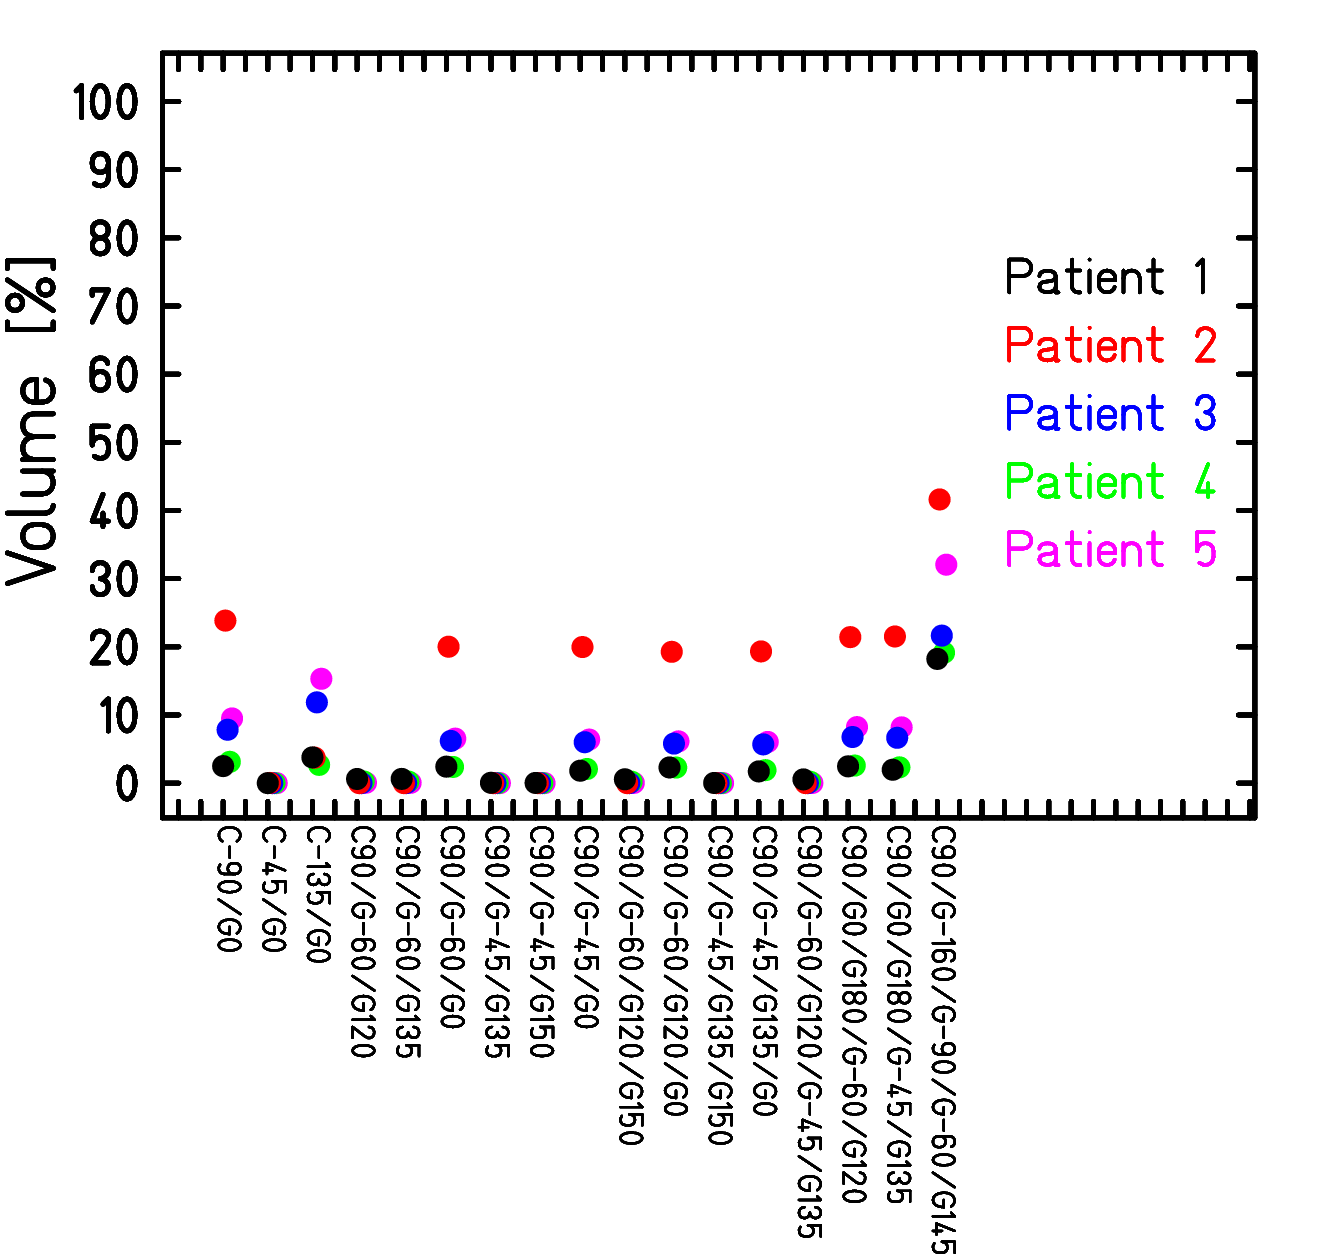
\includegraphics[scale=0.18]{Mayo_Human_BeamDirection_LV_MaxVolume.png}
 }
 \subfigure[Maximum volume: RV]{
 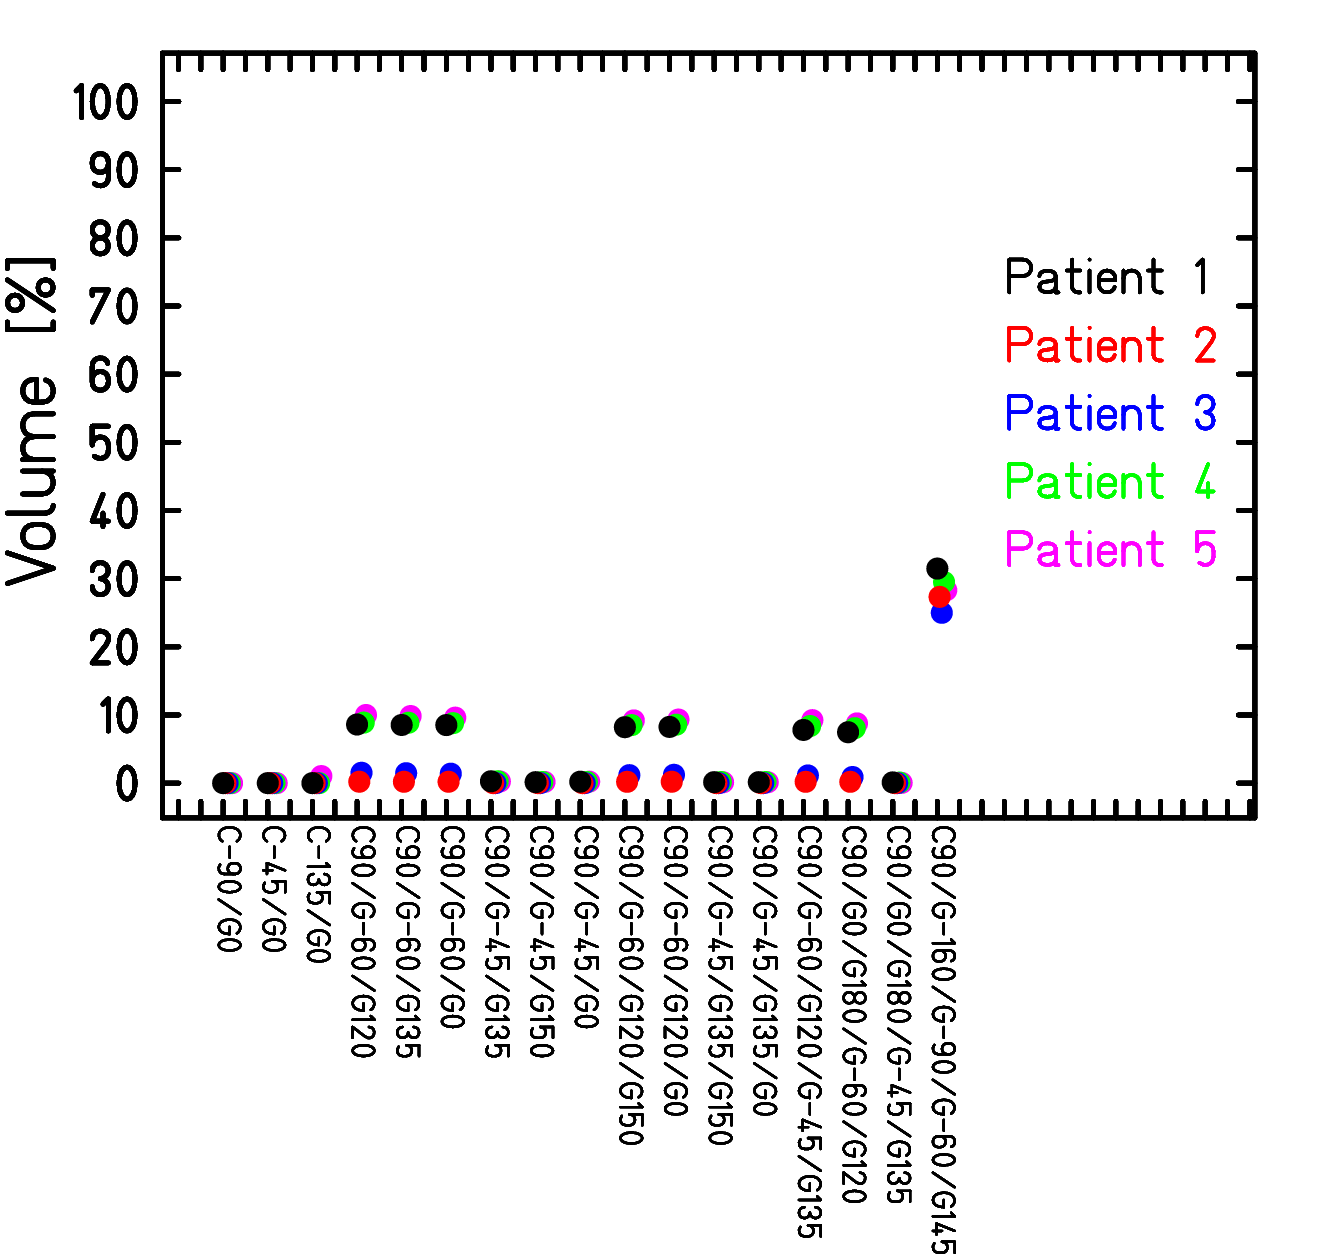
\includegraphics[scale=0.18]{Mayo_Human_BeamDirection_RV_MaxVolume.png}
 }
\caption{Maximal irradiated volume of left ventricle (LV) and right ventricle (RV), respectively, when 
irradiating the LPV and RPV in the five patient data sets with different field numbers and beam directions.}
\label{beamdirection_volume_ventricle}
\end{figure}

\begin{figure}[H]
 \subfigure[Maximum volume: LCA]{
 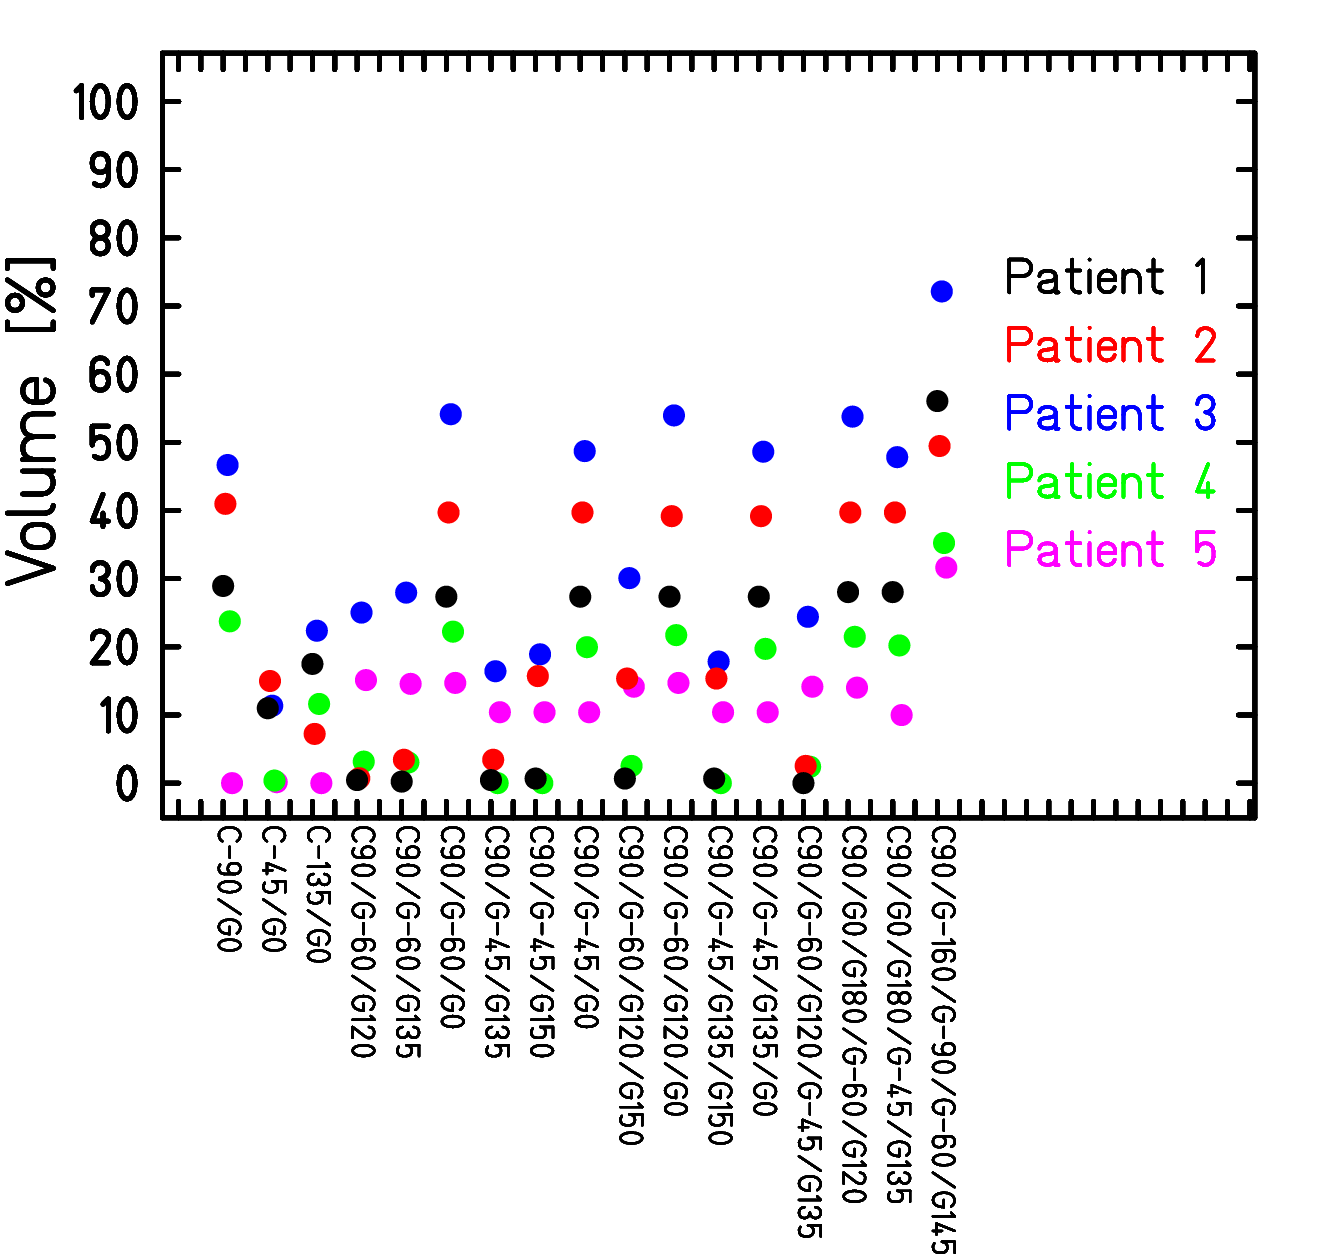
\includegraphics[scale=0.18]{Mayo_Human_BeamDirection_LCA_MaxVolume.png}
 }
 \subfigure[Maximum volume: RCA]{
 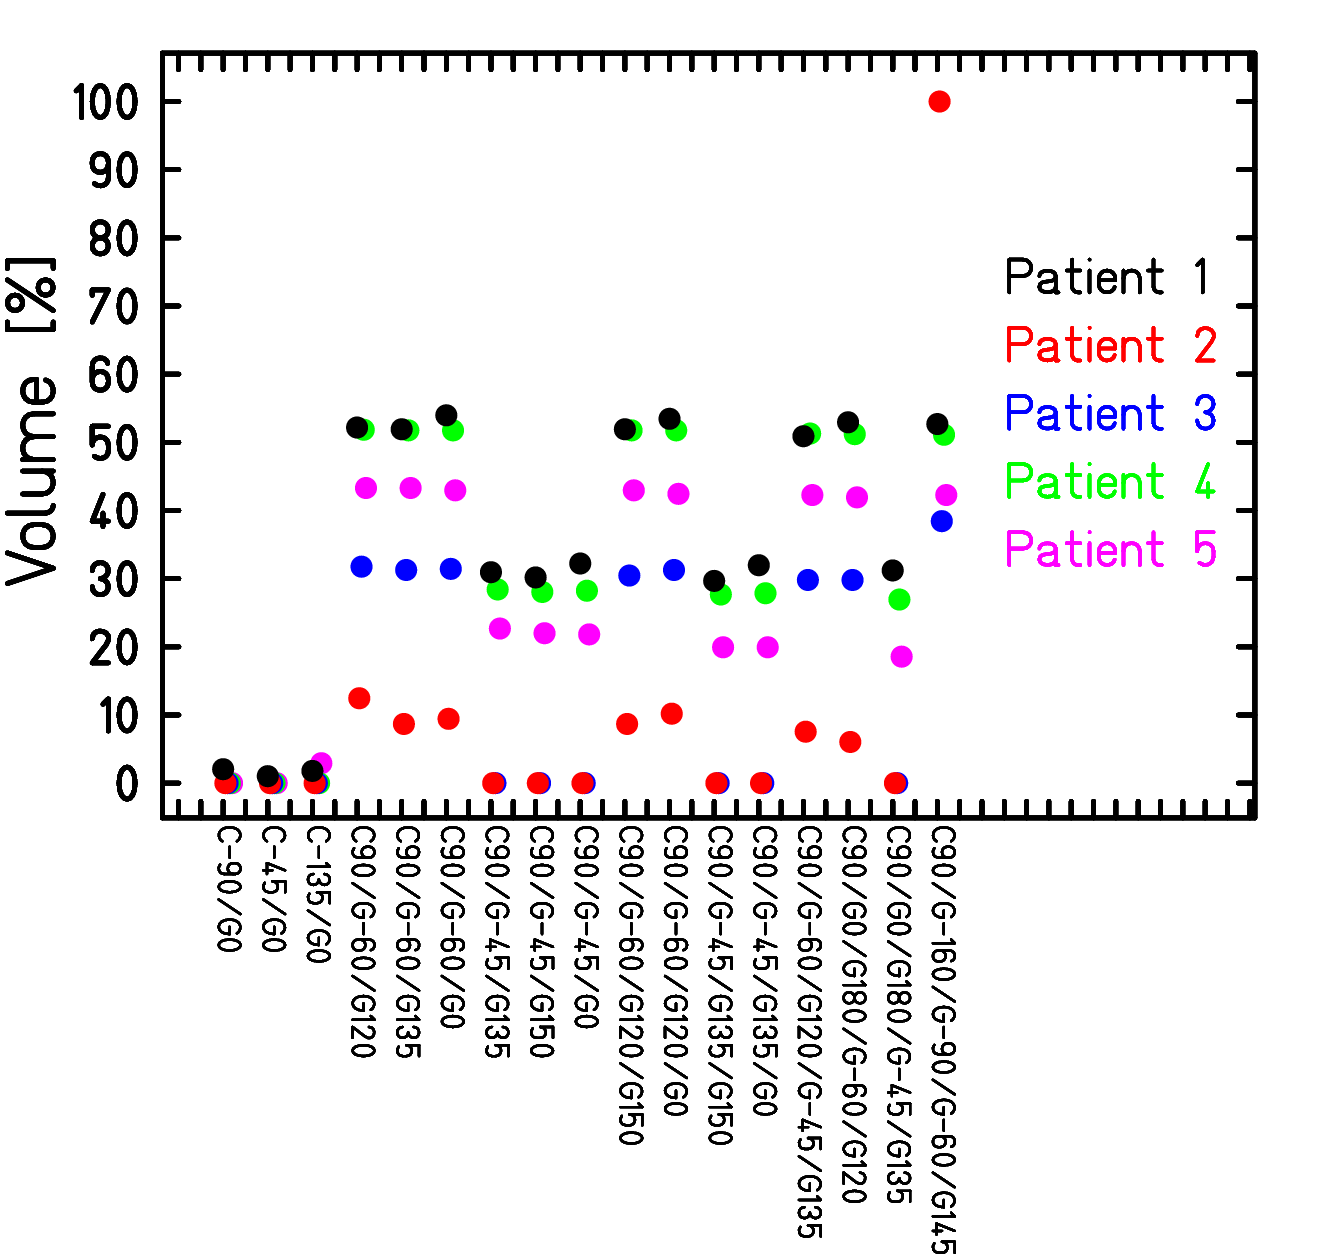
\includegraphics[scale=0.18]{Mayo_Human_BeamDirection_RCA_MaxVolume.png}
 }
\caption{Maximal irradiated volume of left coronary artery (LCA) and right coronary artery (RCA), respectively, when 
irradiating the LPV and RPV in the five patient data sets with different field numbers and beam directions.}
\label{beamdirection_volume_ca}
\end{figure}

\newpage

\vspace*{1cm}

\begin{figure}[H]
\subfigure[Mean dose: LCA]{
 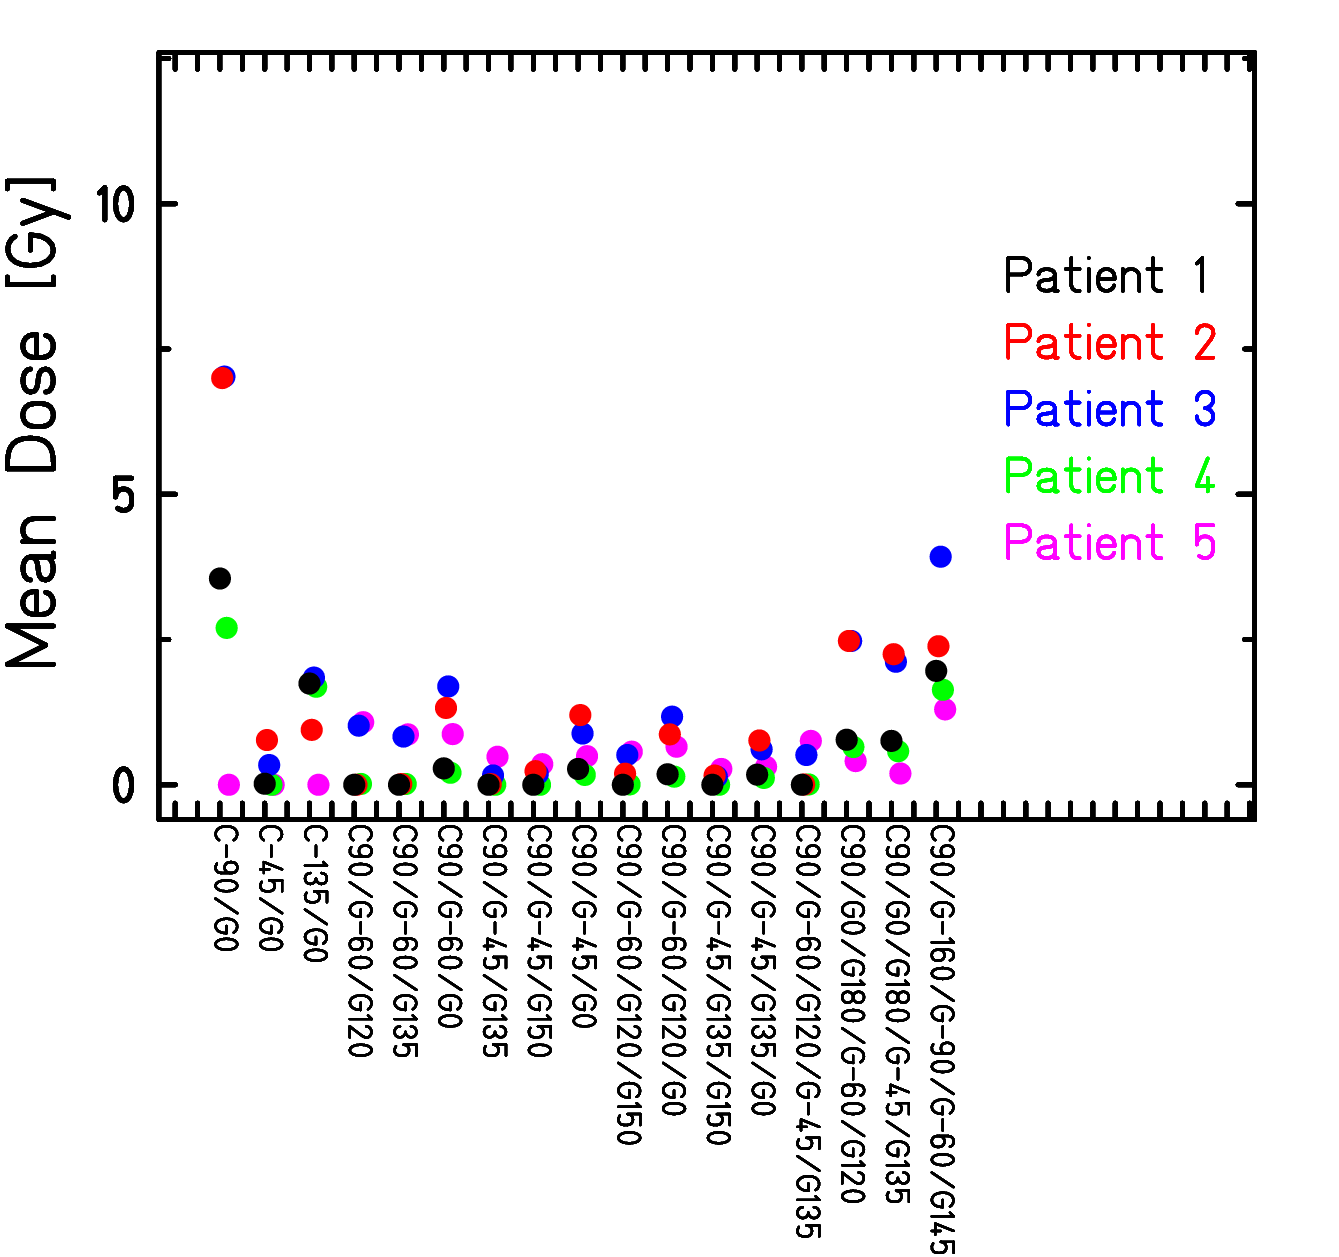
\includegraphics[scale=0.18]{Mayo_Human_BeamDirection_LCA_MeanDose.png}
 }
 \subfigure[Mean dose: RCA]{
 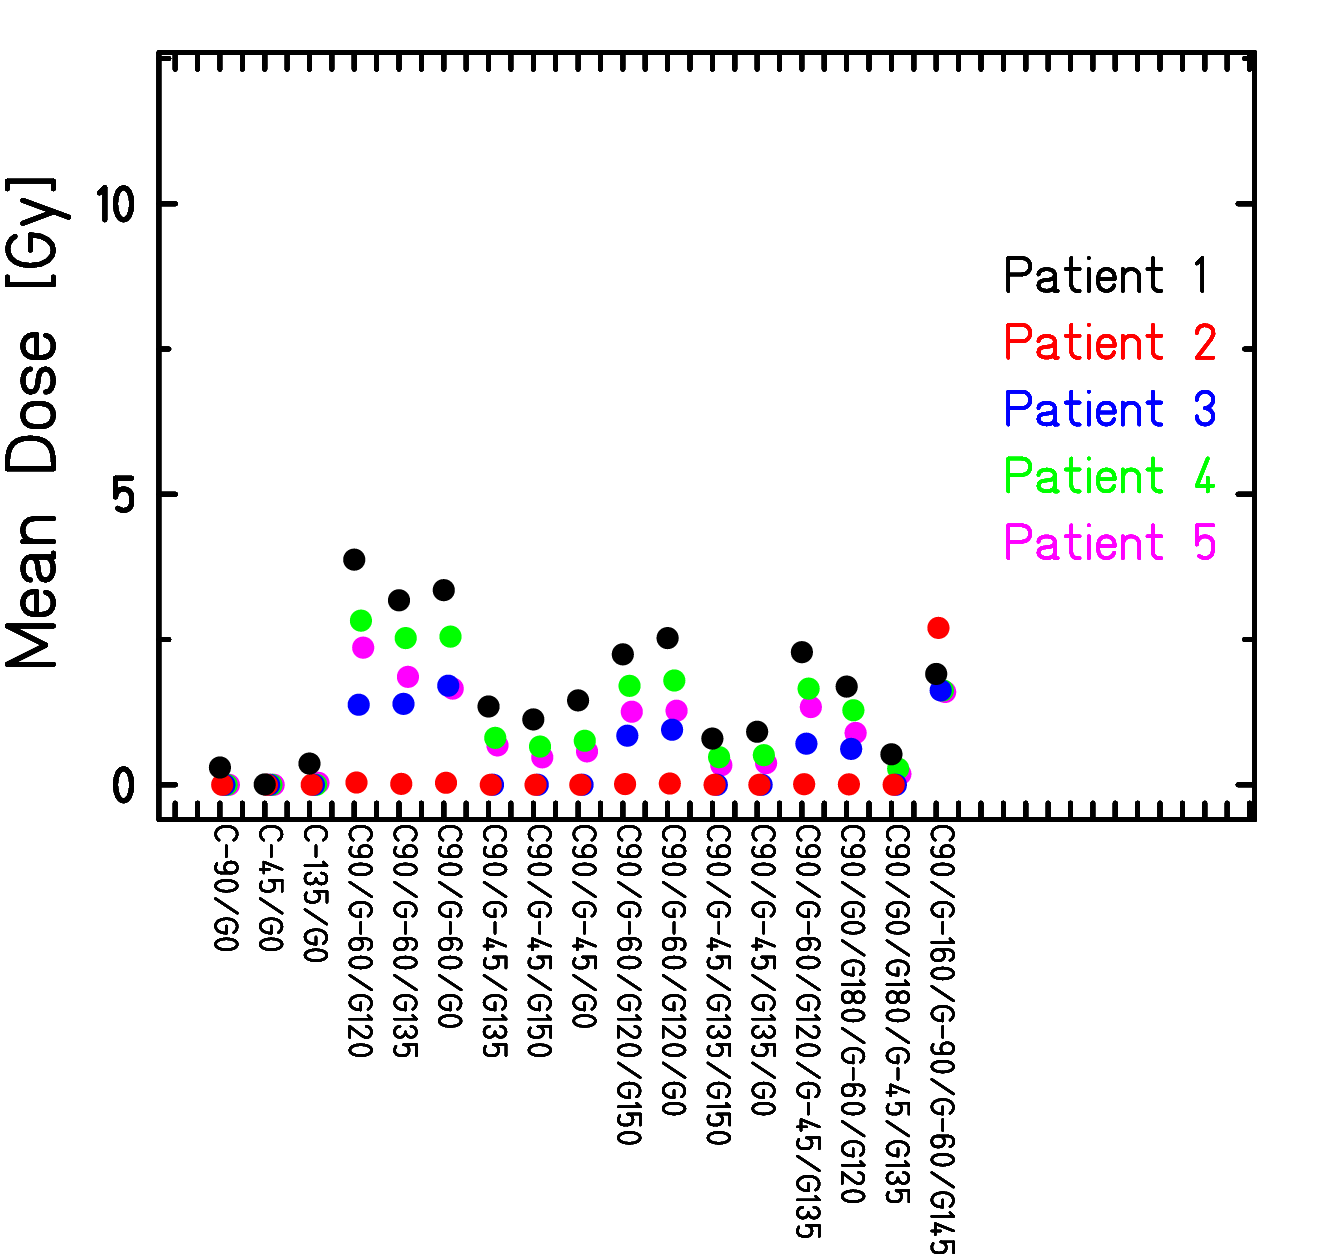
\includegraphics[scale=0.18]{Mayo_Human_BeamDirection_RCA_MeanDose.png}
 }
 \subfigure[Maximum point dose: LCA]{
 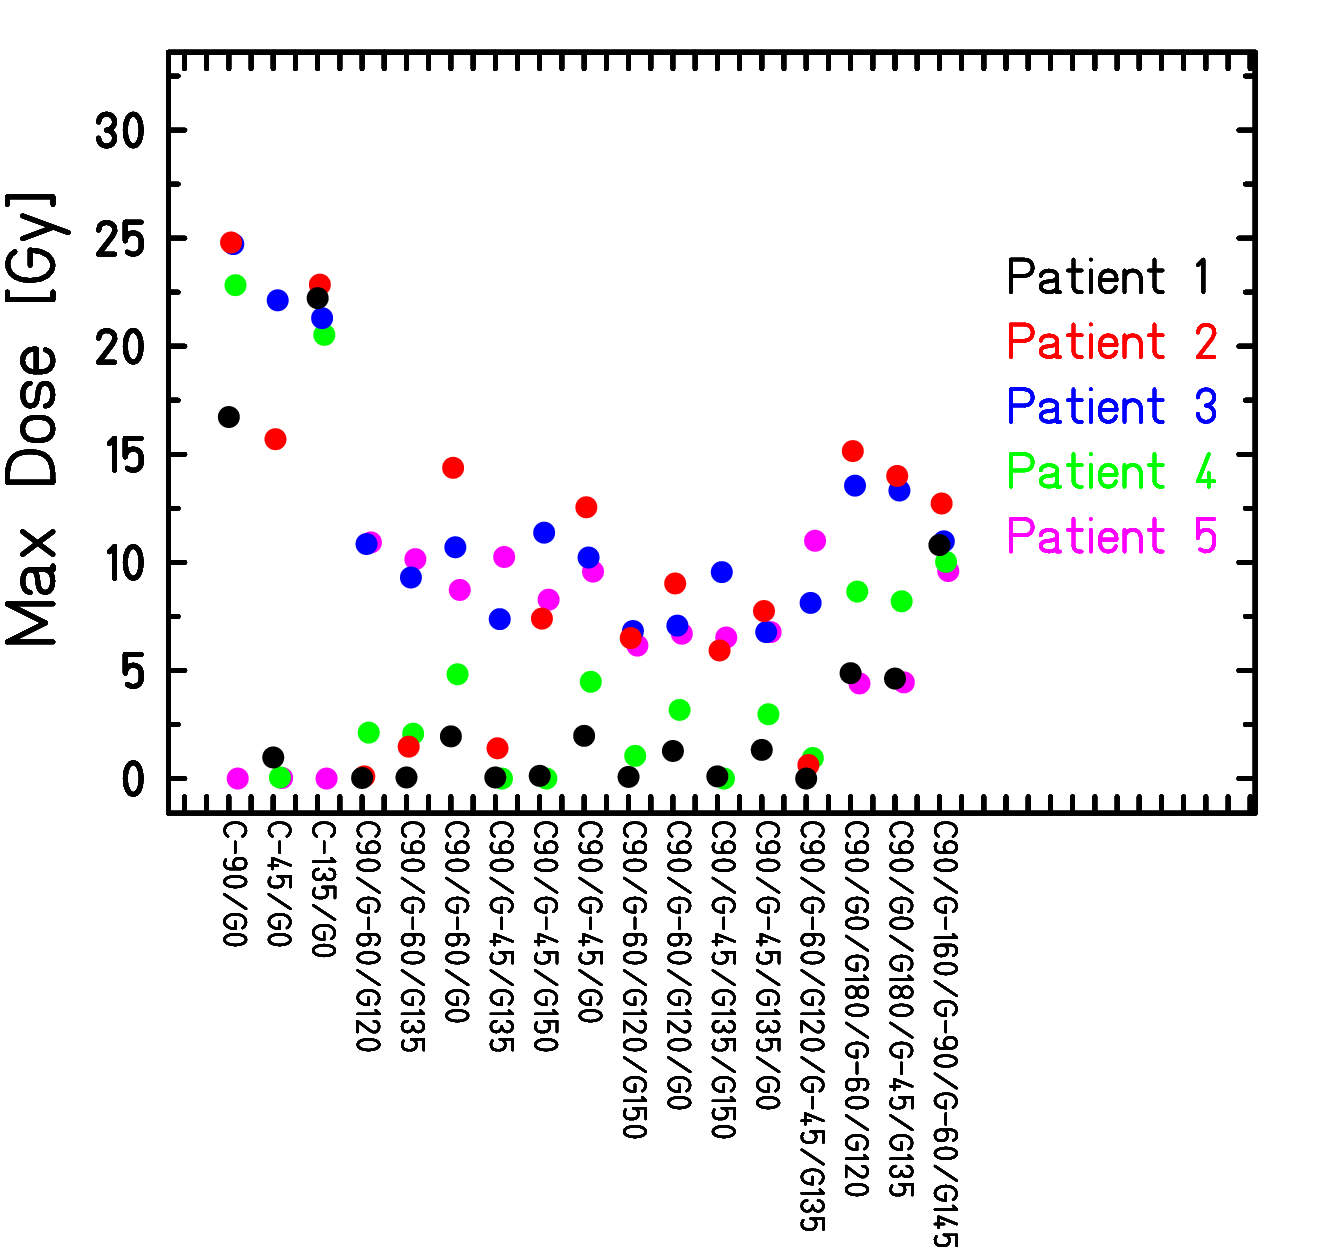
\includegraphics[scale=0.18]{Mayo_Human_BeamDirection_LCA_MaxDose.png}
 }
 \subfigure[Maximum point dose: RCA]{
 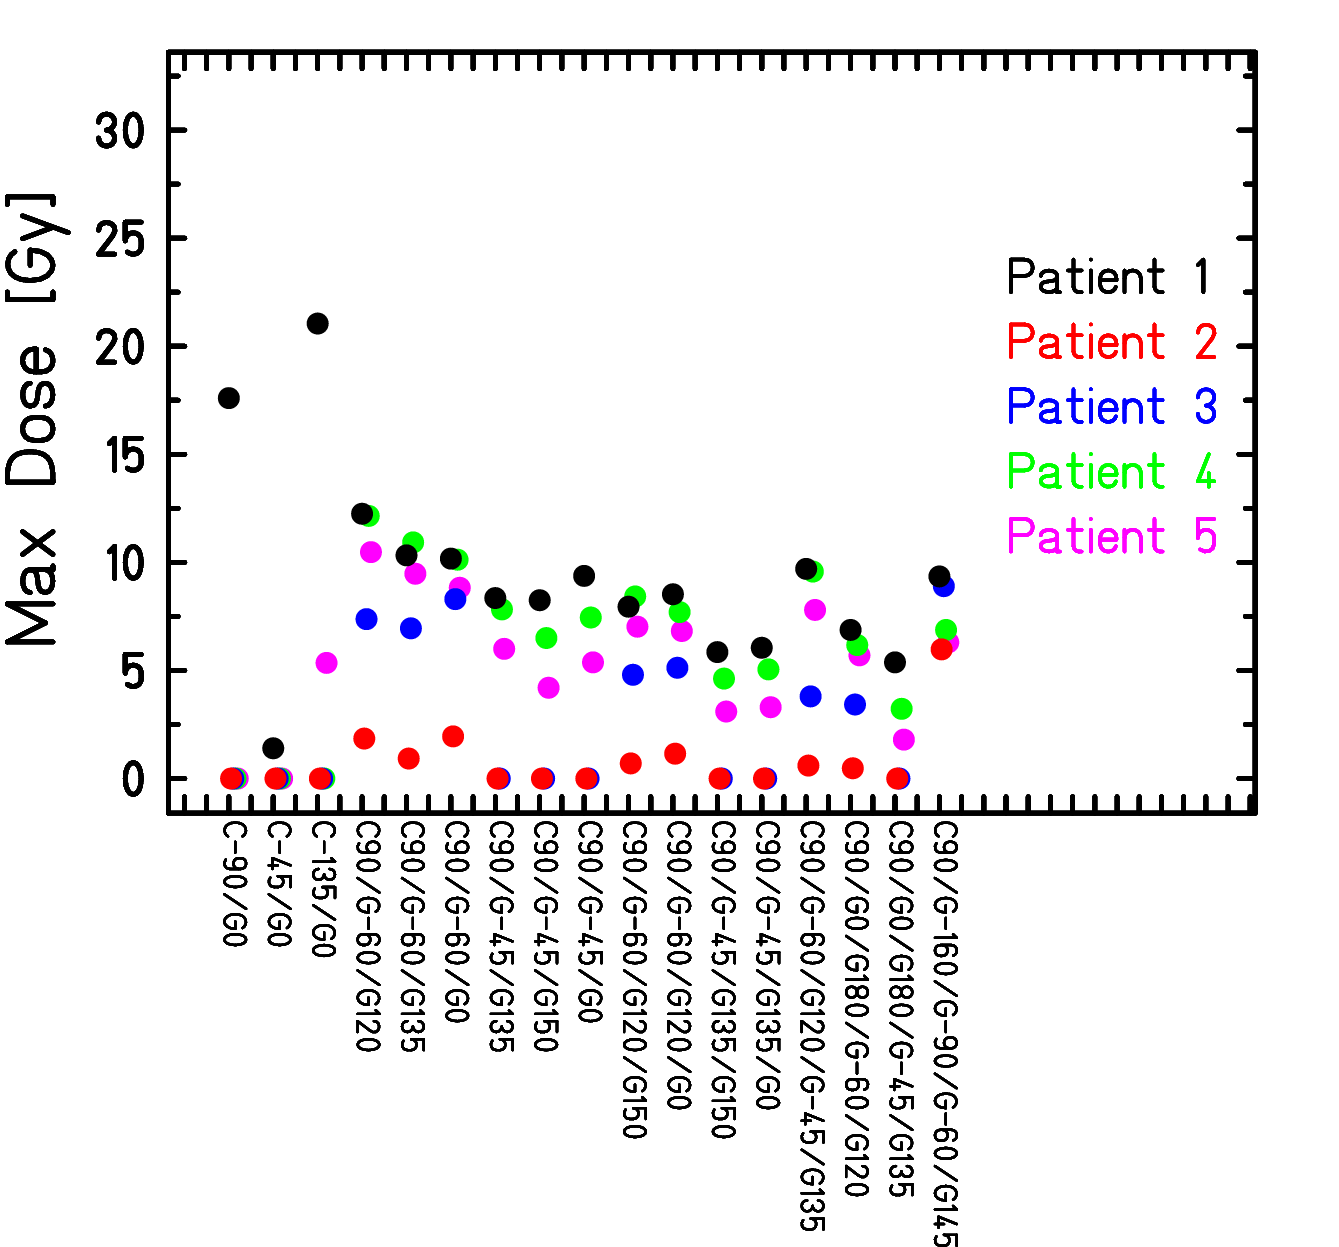
\includegraphics[scale=0.18]{Mayo_Human_BeamDirection_RCA_MaxDose.png}
 }
\caption{Mean dose with standard deviation and maximal point dose of left coronary artery (LCA) and right coronary artery (RCA), respectively, 
when irradiating the LPV and RPV in the five patient data sets with different field numbers and beam directions.}
\label{beamdirection_dose_ca}
\end{figure}

% % \vspace*{-0.6cm}
% 
% While it was not expected to find one beam direction feasible for all five patients, it is striking that no beam position results in a clear 
% benefit for the OAR of the individual patients. This is due to the challenging position of the PV target site, which is in direct proximity 
% to the esophagus and due to the fact that the heart is not only an OAR in this treatment modality, but also the targe site itself. 
% Nevertheless for the analyzed cardiac substructure, especially the radiosensitive LCA, it can be concluded that three beam channels seem to be 
% beneficial for all patients. Regarding the dose deposition in the LCA as well as the maximal irradiated heart volume, combined with the 
% requirement of a robust treatment and hence the benefit of large gantry angles in between different beam channels, a couch angle of 
% -90$^{\circ}$ was chosen together with gantry angles of -45$^{\circ}$, 135$^{\circ}$ and 0$^{\circ}$. These beam channel directions were used 
% for a closer analysis of safety margin limitation as well as for the treatment planning studies for all patients. 

\newpage


\subsection{Safety margin limitations}
\label{safetymarginlimitation}

Figure \ref{static_margin} shows the dose results for the main OAR when irradiating the PVs with no safety margin (0mm) and different additional, 
isotropic safety margins (3mm, 5mm or 7mm). The dose-volume-limits were studied according to the recommendation of RTOG (see table \ref{tab:RTOG}) 
and the limit for each organ is indicated by a dashed line in the plots. Besides an SFUD treatment, IMPT deliveries were also studied. Thereby 
the esophagus was implemented as a critical structure in the optimization process and it was stated that this structure should not receive 
more than 70\% of the physical dose of 25Gy. The results of these two treatment delivery techniques, SFUD irradiation and IMPT, are both shown 
in each plot.\newline
\newline
As expected, the dose to the enclosed OAR increases with increasing safety margin for all patients. This is the case both for SFUD and IMPT 
delivery. Nevertheless the IMPT delivery does lead to a reduced dose deposition in the esophagus. For no safety margin, the median dose over a
all patients is found to 8.5Gy (75th percentile: 12.4Gy), which decreases to 7.0Gy (9.0Gy) with IMPT delivery. 
For 3mm safety margin an SFUD irradiation results to 13.0Gy (18.6Gy) and reduces to 9.3Gy (12.1Gy) for 
IMPT. With 5mm safety margin the RTOG limit of 11.9Gy starts to be exceeded even for IMPT deliveries as it 
results to 11.8Gy (15.1Gy) (compared to 19.0Gy (22.8Gy) with SFUD). For 7mm margin this result further 
increases to 14.3Gy (17.1Gy) (SFUD irradiation: 23.3Gy (24.6Gy)).
% (11.40 $\pm$ 4.04)Gy, which decreases to (6.40 $\pm$ 2.85)Gy with IMPT delivery. For 3mm safety margin, an SFUD 
% irradiation results to (12.20 $\pm$ 4.79)Gy and reduces to (9.40 $\pm$ 2.63)Gy for IMPT, hence still being in the RTOG limits of 11.9 Gy. 
% With 5mm safety margin this dose-volume-limit is exceeded even for IMPT deliveries as it results to (11.95 $\pm$ 2.98)Gy (compared to 
% (16.60 $\pm$ 5.13)Gy for SFUD). For 7mm margin this result further increases to (20.35 $\pm$ 4.06)Gy (SFUD irradiation: (14.15 $\pm$ 2.80)Gy). 
Even though only the esophagus is included in the IMPT optimization process, also other OAR profit from this irradiation mode. This can be 
understood as the beam stopping in front of the esophagus (gantry angle of -45$^{\circ}$) is optimized into having less raster points in the 
IMPT delivery compared to an SFUD irradiation and hence a reduced dose contribution to the total dose delivery. The other beam 
channels (gantry angles of 135$^{\circ}$ and 0$^{\circ}$) are hence optimized into having more raster points compared to the SFUD delivery, 
contributing more to the dose deposition. Adjacent OAR to the esophagus, like trachea and aorta, are thus also receiving a smaller dose 
deposition from the beam channel stopping in proximity to them. As only an IMPT treatment leads to acceptable dose depositions in the esophagus, 
the median dose to the other organs will only be stated for this delivery type. Over all patients the trachea is receiving a median dose of 0Gy 
in all cases, since only patient 2 and 3 are yielding a dose in this critical structure. The 75th percentile is found to 0.4Gy with no safety 
margin and 1.1Gy, 3.0Gy, 6.6Gy for 3mm, 5mm and 7mm, respectively. 
% up to 0.35Gy for no safety margin, and up to 1.05Gy, 1.87Gy, 6.11Gy for 3mm, 5mm and 7mm, respectively. 
All of these dose deposition are under the recommended dose-volume-limit for the trachea (10.5Gy for 4cm$^{3}$). 
For the aorta an irradiation with no safety margin leads to a median dose deposition of 6.5Gy (8.5Gy), while 8.3Gy (10.6Gy), 
9.8Gy (12.3Gy) and 11.3Gy (14.0Gy) are deposited with 3mm, 5mm and 7mm margin.
% (7.25 $\pm$ 1.51)Gy, while (8.90 $\pm$ 1.86)Gy, (10.30 $\pm$ 2.08)Gy and (11.90 $\pm$ 2.38)Gy are deposited with 3mm, 5mm and 7mm margin. 
All these results are far under the critical dose-volume limit of 31Gy for 10cm$^{3}$. It can thus be concluded that trachea and aorta do not 
receive a critical dose deposition while treating the PVs with a dose of 25Gy. For the heart the dose-volume limits are much more critical. 
% An average of (76.60 $\pm$ 12.78)Gy was yielded for no safety margin and (89.60 $\pm$ 9.52)Gy, (92.60 $\pm$ 7.94)Gy and (94.20 $\pm$ 6.82)Gy 
% for 3mm, 5mm and 7mm margin, respectively. 
A mean of 18.3Gy (22.8Gy) was yielded for no safety margin and 23.0Gy (24.9Gy), 24.3Gy (25.0Gy) and 24.8Gy (25.0Gy) for 3mm, 5mm and 7mm 
margin, respectively.
Hence all studied irradiations by far exceed the dose-volume limit of 16Gy for 15cm$^{3}$. A close analysis of the radiosensitive cardiac 
substructures is presented in figure \ref{static_margin_dose_heart} - figure \ref{static_margin_dose_coronary_arteries}. 
% 
% %%%%%%%%%%%%%%%%%%%%%%%%%%%%%%%%%%%
% 
% - with IMPT to esophagus within dose-volume-limits for margins of 3 mm
% - one patient (patient 2) exceeds
% - different parameters for IMPT used: before maximum dose fraction (MDF) 0.7 and weightfactor of 0.75. Now tried: MDF = 0.3 and WF=2. 
% - displayed as triangle in plot 
% - it can be further optimized to better spare esophagus
% - nevertheless it should be kept in mind that this also influences dose deposition to other OAR
% - leads to decreased dose-volume in trachea (from 1.5 Gy in 4 cc to 0.5 Gy in 4 cc) but in aorta e.g. higher dose (from 12.5 Gy in 10 cc 
%   to 13 Gy in 10 cc)
% - this multicriteria optimization, or Pareto optimization, is discussed for example in \cite{Mon08} \cite{Chen12} 
% 
% %%%%%%%%%%%%%%%%%%%%%%%%%%%%%%%%%%%


%%%%%%%% DOSE TO OAR

% \vspace*{-0.4cm}

\begin{figure}[H]
\subfigure[Esophagus]{
 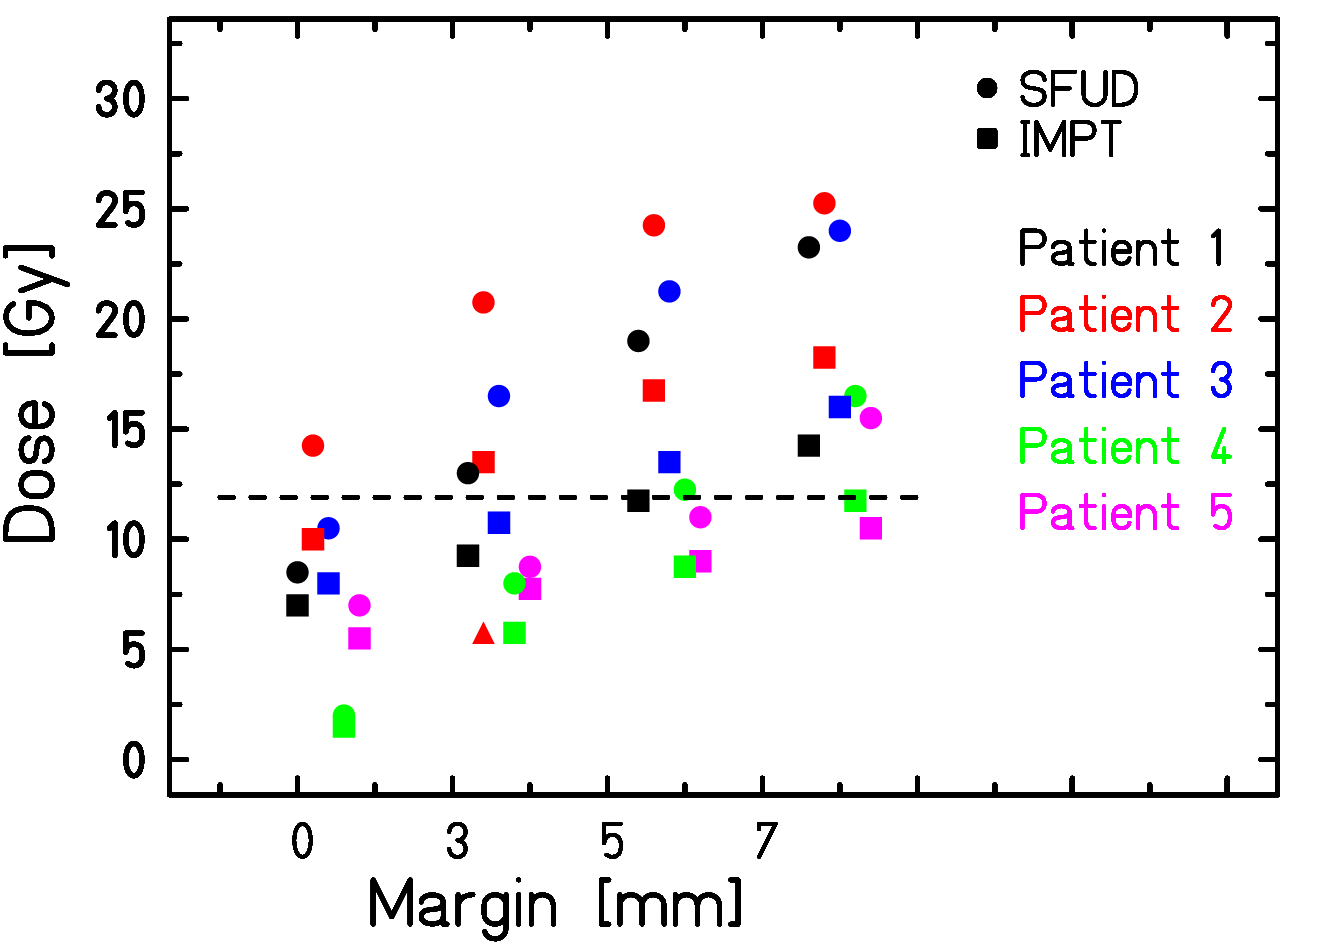
\includegraphics[scale=0.18]{Mayo_Human_ESO_alternativeLimit_diffIMPT.png}
 }
 \subfigure[Trachea]{
 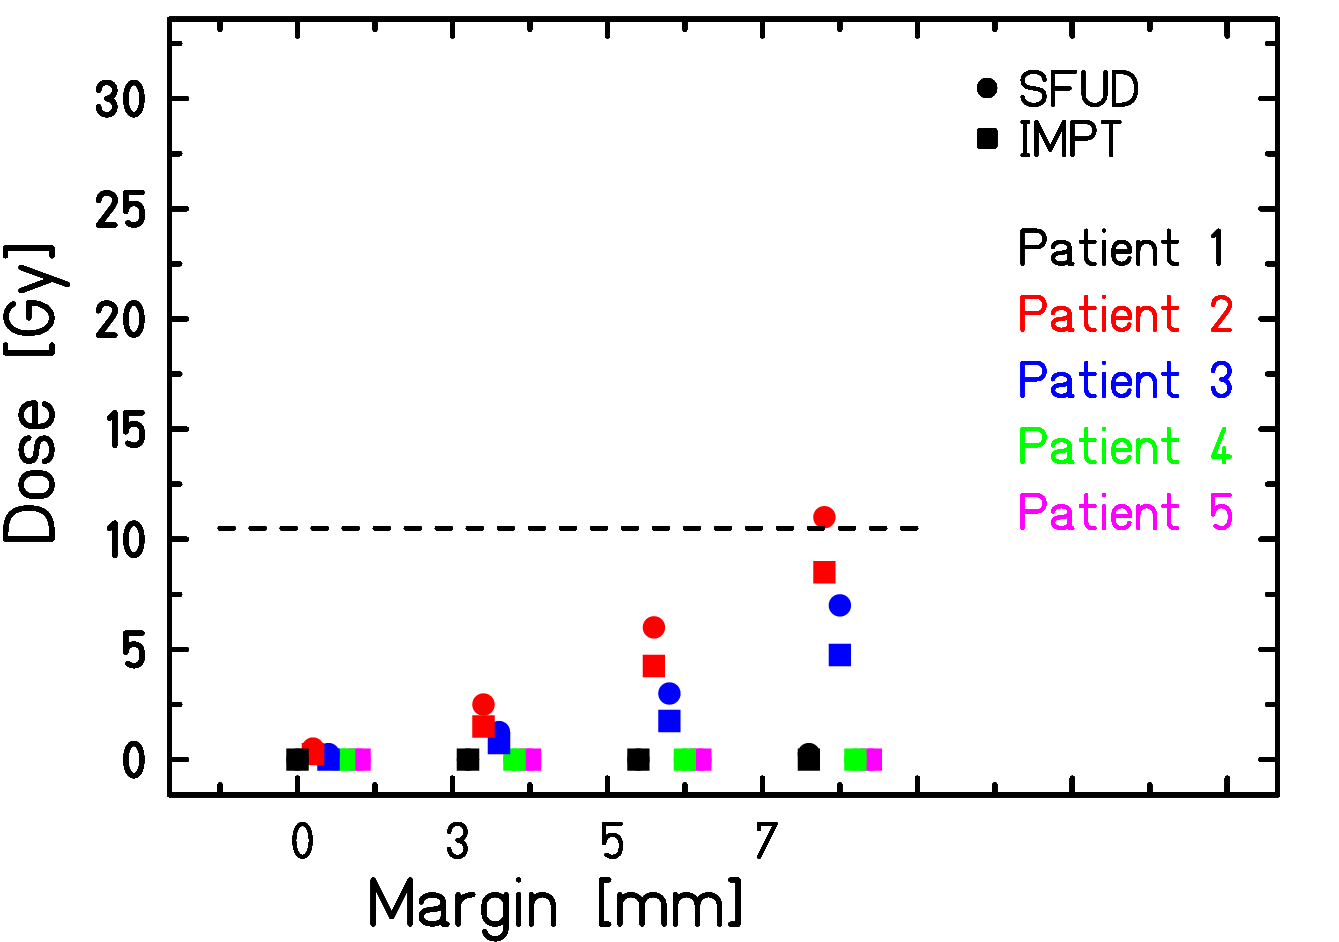
\includegraphics[scale=0.18]{Mayo_Human_TRACHEA.png}
 }
  \subfigure[Heart]{
 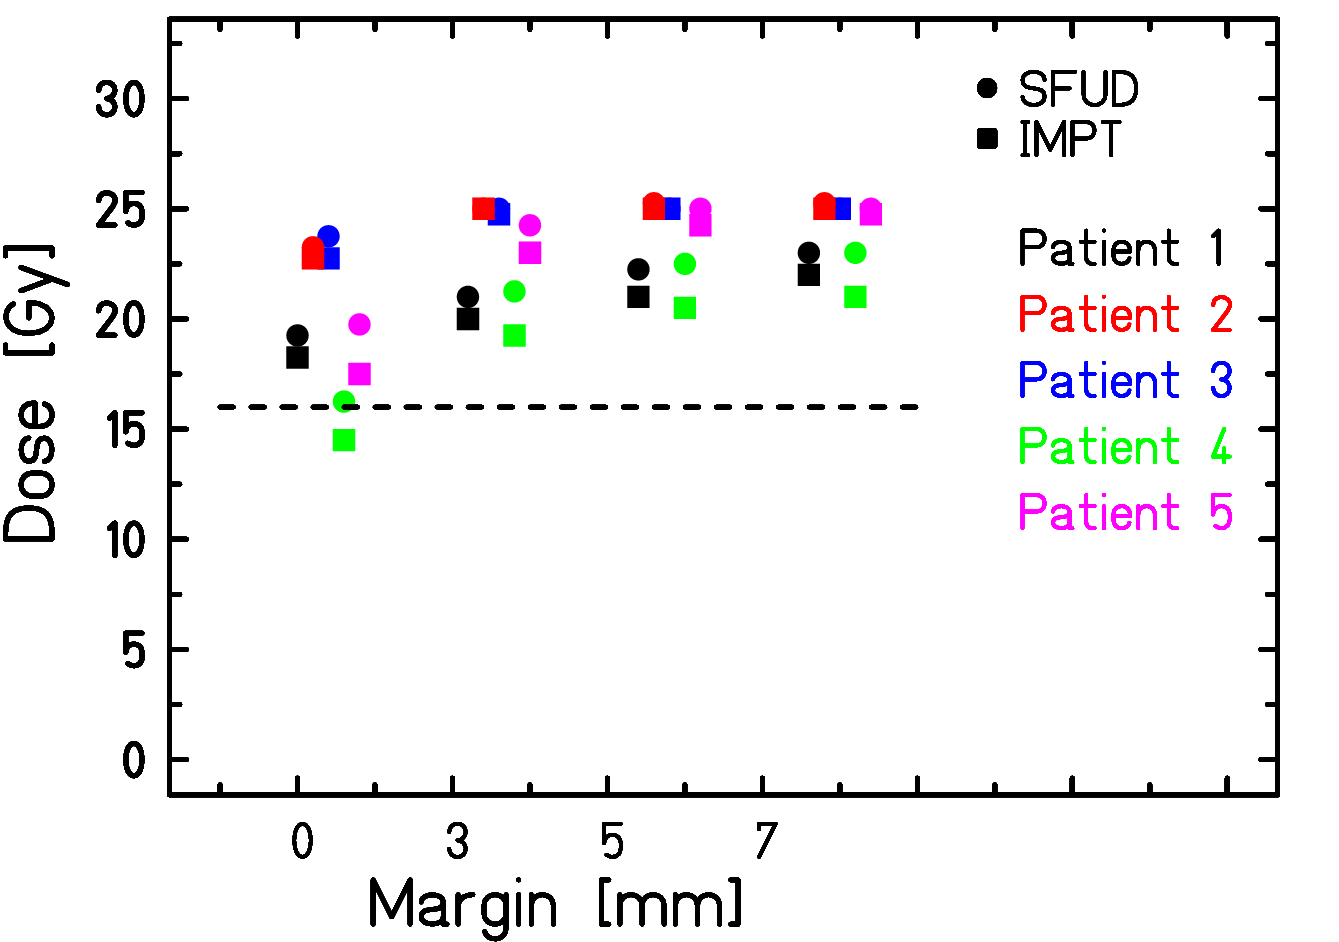
\includegraphics[scale=0.18]{Mayo_Human_HEARTwoOverlap.png}
 }
  \subfigure[Aorta]{
 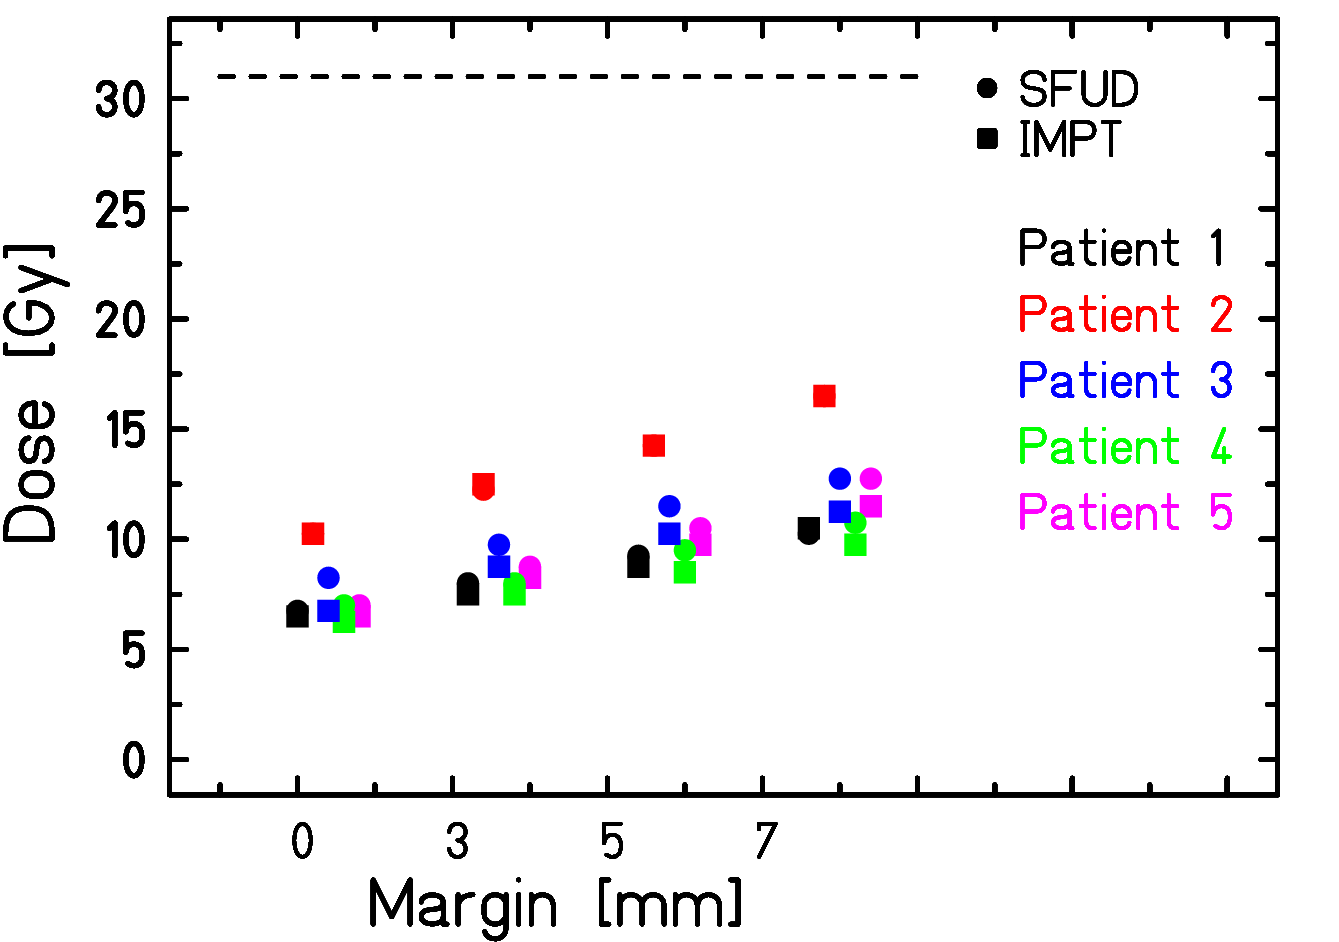
\includegraphics[scale=0.18]{Mayo_Human_AORTA.png}
 }
% \subfigure[Left coronary artery]{
%  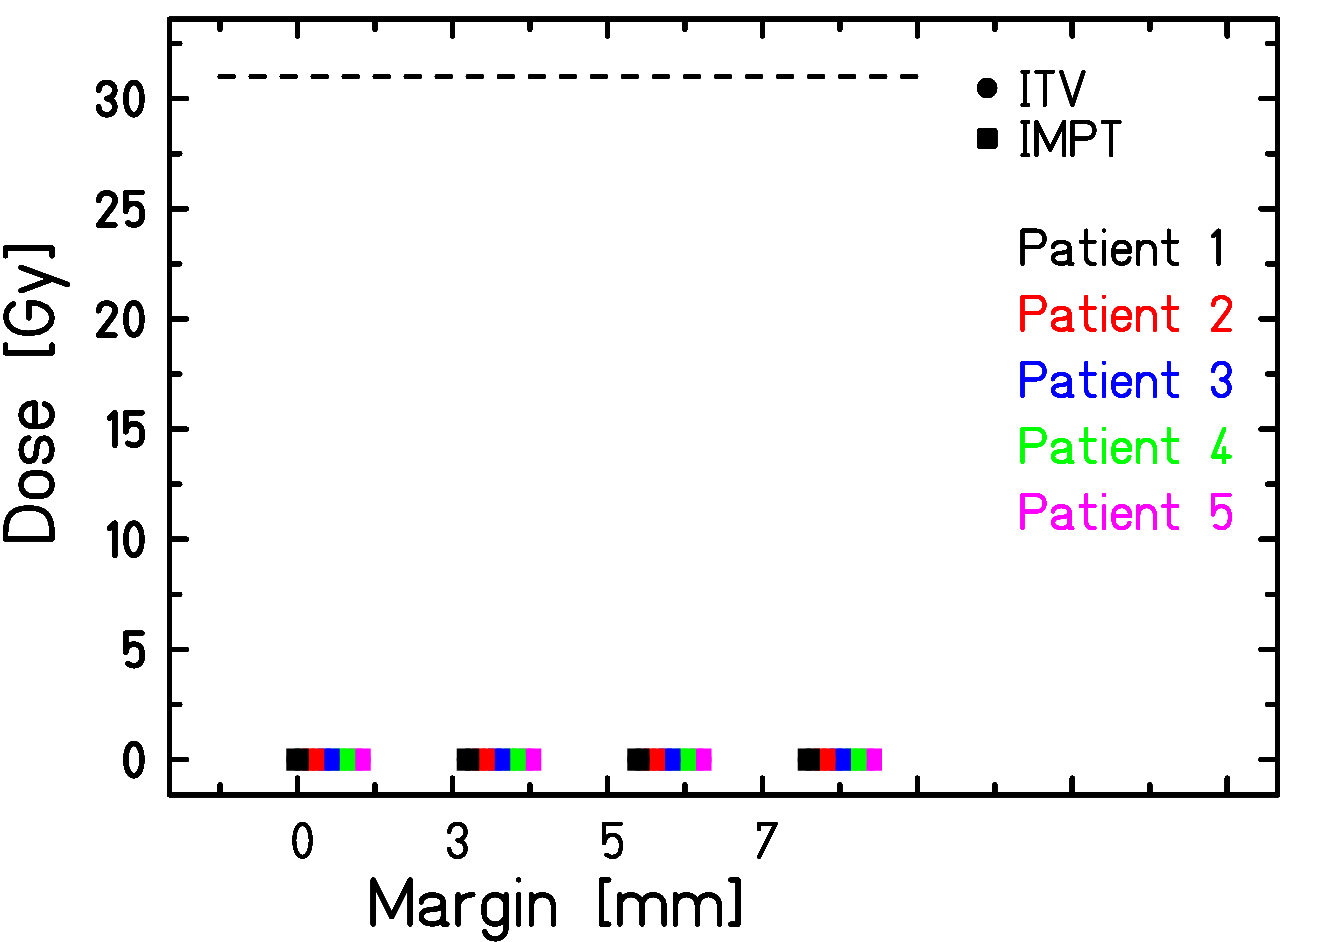
\includegraphics[scale=0.18]{Mayo_Human_LCA.png}
%  }
%  \subfigure[Right coronary artery]{
%  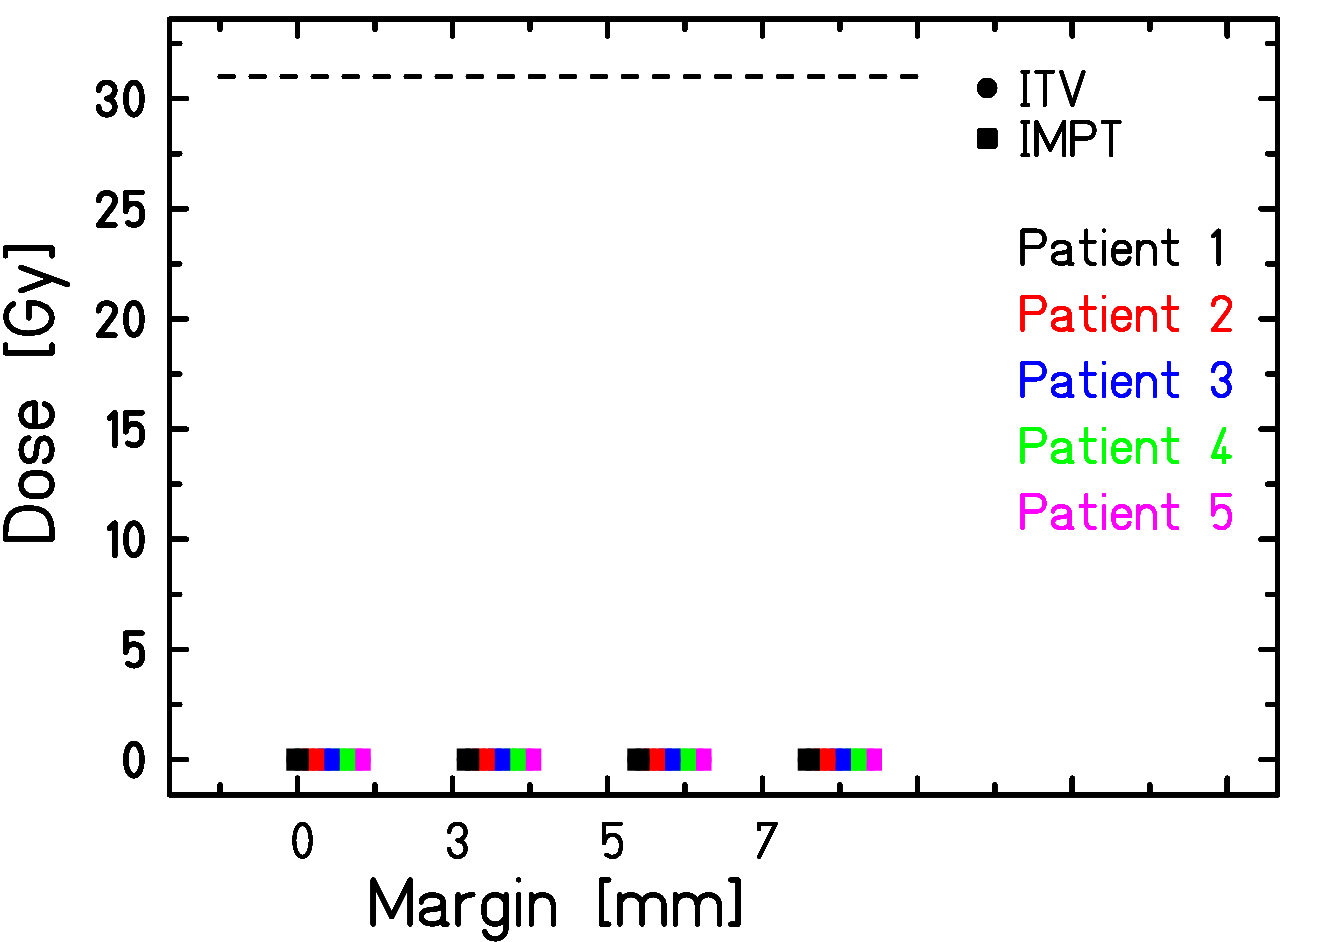
\includegraphics[scale=0.18]{Mayo_Human_RCA.png}
%  }
\caption{Dose-volume data of different OAR when irradiating the PVs in five patient data sets with different margins and two 
different delivery techniques (SFUD and IMPT).
The dose-volume-limit for each critical organ is indicated with a dashed line in each plot, respectively.}
\label{static_margin}
\end{figure}

% %%%%%%%%%%%%%%%%%%%%%%%%%%%%%%%%%%%
% 
% - with IMPT to esophagus within dose-volume-limits for margins of 3 mm
% - one patient (patient 2) exceeds
% - different parameters for IMPT used: before maximum dose fraction (MDF) 0.7 and weightfactor of 0.75. Now tried: MDF = 0.3 and WF=2. 
% - displayed as triangle in plot 
% - it can be further optimized to better spare esophagus
% - nevertheless it should be kept in mind that this also influences dose deposition to other OAR
% - leads to decreased dose-volume in trachea (from 1.5 Gy in 4 cc to 0.5 Gy in 4 cc) but in aorta e.g. higher dose (from 12.5 Gy in 10 cc 
%   to 13 Gy in 10 cc)
% - this multicriteria optimization, or Pareto optimization, is discussed for example in \cite{Mon08} \cite{Chen12} 
% 
% %%%%%%%%%%%%%%%%%%%%%%%%%%%%%%%%%%%

It should further be noted that another IMPT parameter set was studied for the esophagus of patient 2 with 3mm Margin. While the other four 
patients are within the dose-volume limit with this safety margin this patient exceeds the limit 
by 1.6Gy. The result could be improved by using another parameter set (maximum dose fraction of 30\% and a weighting factor of two), which 
is represented as a triangle in plot \ref{static_margin}. The dose can be drastically reduced to 5.8Gy for 5cm$^{3}$ esophagus. 
% Nevertheless, this leads to an increased dose deposition in the other OAR so that e.g. the aorta receives a slightly higher dose (13 Gy 
% compared to 12.5Gy in 10cm$^{3}$). 
It can thus be concluded that patient individual optimization can further improve the stated results. 
However, as the majority of the patients did not exceed the limit for 3mm margin, the previously stated parameters for IMPT treatment were 
used in further analysis.\newline
\newline
Closer analysis of the dose deposition in the heart can be seen in figure \ref{static_margin_dose_heart}. The mean deposited dose in the 
heart does not increase with the size of the safety margins. Furthermore only a small difference in between SFUD and IMPT irradiation can be observed. 
The median value of the mean dose over all patients for an IMPT irradiation with no safety margin is found to 1.0Gy (75th percentile: 1.1Gy). 
For the irradiation of the PVs with safety margin it results to 1.3Gy (1.5Gy) for 3mm, 1.4Gy (1.6Gy) for 
5mm and 1.5Gy (1.6Gy) for 7mm, respectively. 
% % The median value of the mean dose over all patients for an SFUD irradiation with no safety margin is found to 1.02Gy (75th percentile: 1.27Gy) 
% % compared to 0.97Gy (75th percentile: 1.12Gy) with IMPT. For the irradiation of the PVs with safety margin it results to 1.34Gy (75th 
% % percentile: 1.69Gy) versus 1.26Gy (75th percentile: 1.48Gy), 1.51Gy (75th percentile: 1.84Gy) versus 1.43Gy (75th percentile: 1.59Gy) and 
% % 1.64Gy (75th percentile: 1.90Gy) versus 1.54Gy (75th percentile: 1.63Gy) for 3mm, 5mm and 7mm, respectively. 
While also the maximum point dose does not increase with added safety margin, it can be seen that IMPT treatment does lead to a higher point 
dose compared to an SFUD irradiation. A comparison of the median maximum point dose and the 75th percentile over all patients and for all 
margin cases is presented in table \ref{tab:maxdose_heart}.

\vspace*{-0.3cm}

\begin{table}[H]
  \centering
  \caption{Median and 75th percentile of maximum point dose to the heart.}
  \begin{tabular}{|c||c|c|}
    \hline\hline
    Margin & SFUD: median (75th percentile) [Gy] & IMPT: median (75th percentile) [Gy] \\
    \hline
    0 mm & 26.9 (26.9) & 27.58 (29.4) \\
    3 mm & 26.2 (26.6) & 28.35 (29.0) \\
    5 mm & 26.5 (26.6) & 28.00 (28.8) \\
    7 mm & 26.2 (27.7) & 26.80 (27.7) \\
    \hline\hline
  \end{tabular}
  \label{tab:maxdose_heart}
\end{table}

% \begin{table}[H]
%   \centering
%   \caption{Mean maximum point dose to the heart.}
%   \begin{tabular}{|c|c|c|}
%     \hline\hline
%     Margin & SFUD [Gy] & IMPT [Gy] \\
%     \hline
%     0 mm & 26.82 $\pm$ 0.30 & 28.11 $\pm$ 1.32 \\
%     3 mm & 26.60 $\pm$ 0.72 & 28.58 $\pm$ 1.01 \\
%     5 mm & 26.57 $\pm$ 0.60 & 27.97 $\pm$ 1.12 \\
%     7 mm & 26.88 $\pm$ 0.99 & 27.19 $\pm$ 0.64 \\
%     \hline\hline
%   \end{tabular}
%   \label{tab:maxdose_heart}
% \end{table}

% % Over all patients the mean maximum point dose with an SFUD treatment results to (26.82 $\pm$ 0.30)Gy for 
% % no margin and (26.60 $\pm$ 0.72)Gy for 3mm margin, (26.57 $\pm$ 0.60)Gy for 5mm margin, (26.88 $\pm$ 0.99)Gy for 7mm, respectively. With an 
% % IMPT treatment a slightly higher mean maximum point dose is observed in all cases. It yields to (28.11 $\pm$ 1.32)Gy, (28.58 $\pm$ 1.01)Gy, 
% % (27.97 $\pm$ 1.12)Gy and (27.19 $\pm$ 0.64)Gy with no margin and 3mm, 5mm, 7mm, respectively. 
The highest maximum point dose (30.3Gy) was deposited in the heart of patient 3 with a margin of 3mm. In comparison, the SFUD result for this 
case is 26.6Gy. As esophagus and the other adjacent OAR (trachea, aorta) receive in general less dose with IMPT due to the intensity reduction 
in one beam channel direction, the other beam channels have to deposit more particles. Especially gantry angle 0$^{\circ}$, which traverses 
the heart, is hence leading to an increased dose deposition in the heart. Since this beam channel direction has to penetrate only a small 
volume of the heart, the maximal irradiated volume shows a slight improvement in IMPT delivery compared to SFUD irradiation. The results are 
presented in table \ref{tab:maxvolume_heart}.

\vspace*{-0.3cm}

\begin{table}[H]
  \centering
  \caption{Median and 75th percentile of maximum irradiated volume of the heart.}
  \begin{tabular}{|c||c|c||c|c|}
    \hline\hline
    Margin & SFUD: median (75th percentile) [\%] & IMPT: median (75th percentile) [\%]\\
    \hline
    0 mm & 17.2 (20.0) & 15.7 (18.9) \\
    3 mm & 19.4 (22.6) & 17.4 (21.2) \\
    5 mm & 20.7 (24.9) & 18.5 (23.2) \\
    7 mm & 21.8 (26.4) & 19.9 (24.4) \\
    \hline\hline
  \end{tabular}
  \label{tab:maxvolume_heart}
\end{table}

% \begin{table}[H]
%   \centering
%   \caption{Mean maximum irradiated volume of the heart.}
%   \begin{tabular}{|c|c|c|}
%     \hline\hline
%     Margin & SFUD [\%] & IMPT [\%] \\
%     \hline
%     0 mm & 17.14 $\pm$ 2.82 & 16.28 $\pm$ 2.76 \\
%     3 mm & 19.56 $\pm$ 3.09 & 18.44 $\pm$ 2.99 \\
%     5 mm & 21.34 $\pm$ 3.34 & 20.01 $\pm$ 3.20 \\
%     7 mm & 20.01 $\pm$ 3.20 & 21.42 $\pm$ 3.25 \\
%     \hline\hline
%   \end{tabular}
%   \label{tab:maxvolume_heart}
% \end{table}

% % The mean maximum irradiated volume over all patients is found to (17.14 $\pm$ 2.82)\% with SFUD compared to (16.28 $\pm$ 2.76)\% 
% % in IMPT with no safety margin. For the additional studied margins the following results were found: (19.56 $\pm$ 3.09)\% versus 
% % (18.44 $\pm$ 2.99)\%, (21.34 $\pm$ 3.34)\% versus (20.01 $\pm$ 3.20)\% and (22.81 $\pm$ 3.38)\% versus (21.42 $\pm$ 3.25)\% for 3mm, 5mm and 
% % 7mm margin SFUD and IMPT treatment, respectively.\newline
% % \newline


%%%%%%%% DOSE TO THE HEART

\newpage

\begin{figure}[H]
\begin{center}
\subfigure[Heart: mean dose]{
 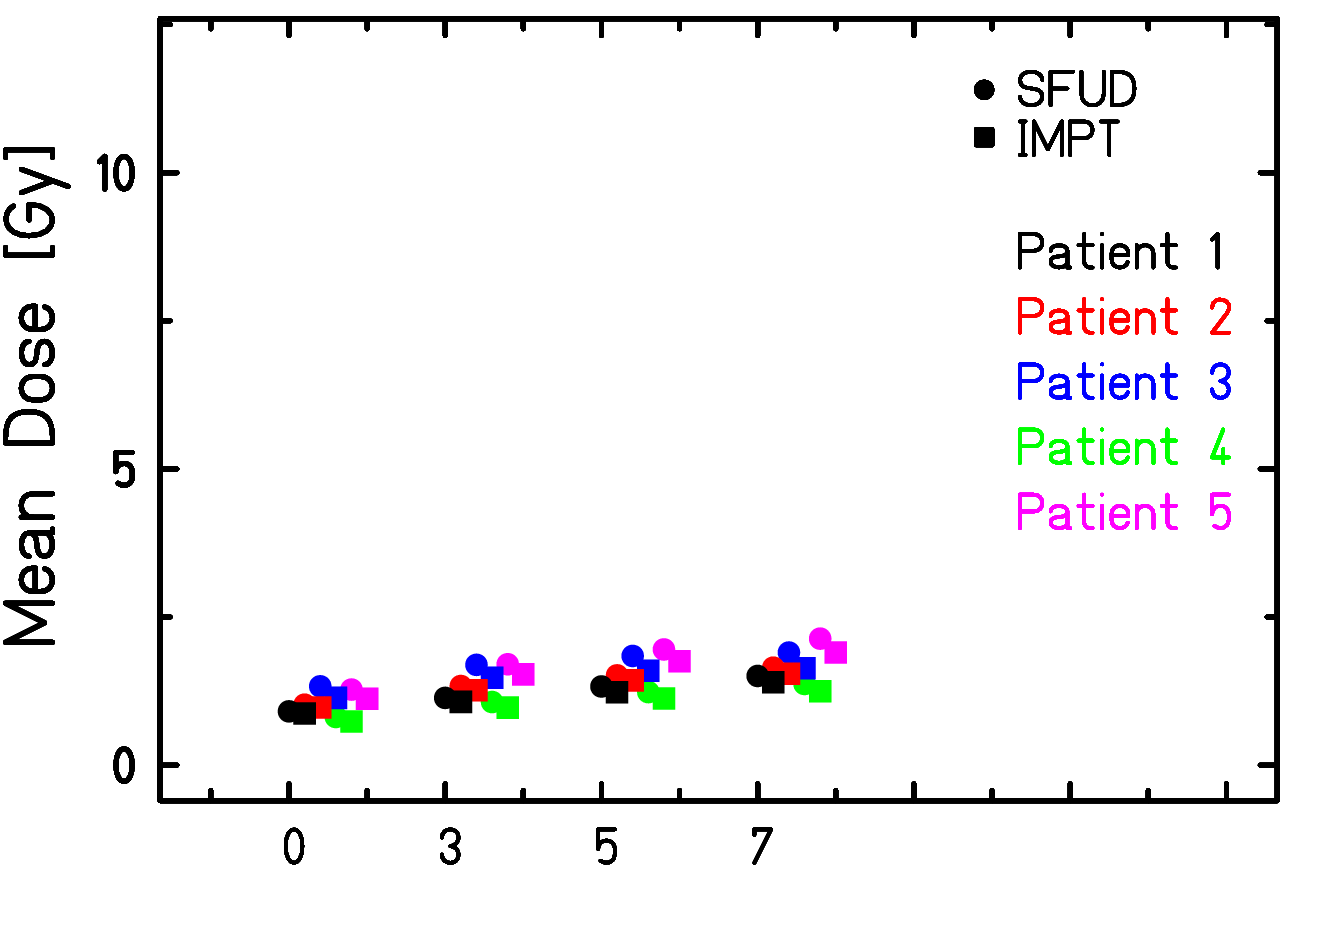
\includegraphics[scale=0.18]{Mayo_Human_HEARTwoOverlap_MeanDose.png}
 }
 
 \subfigure[Heart: maximum point dose]{
 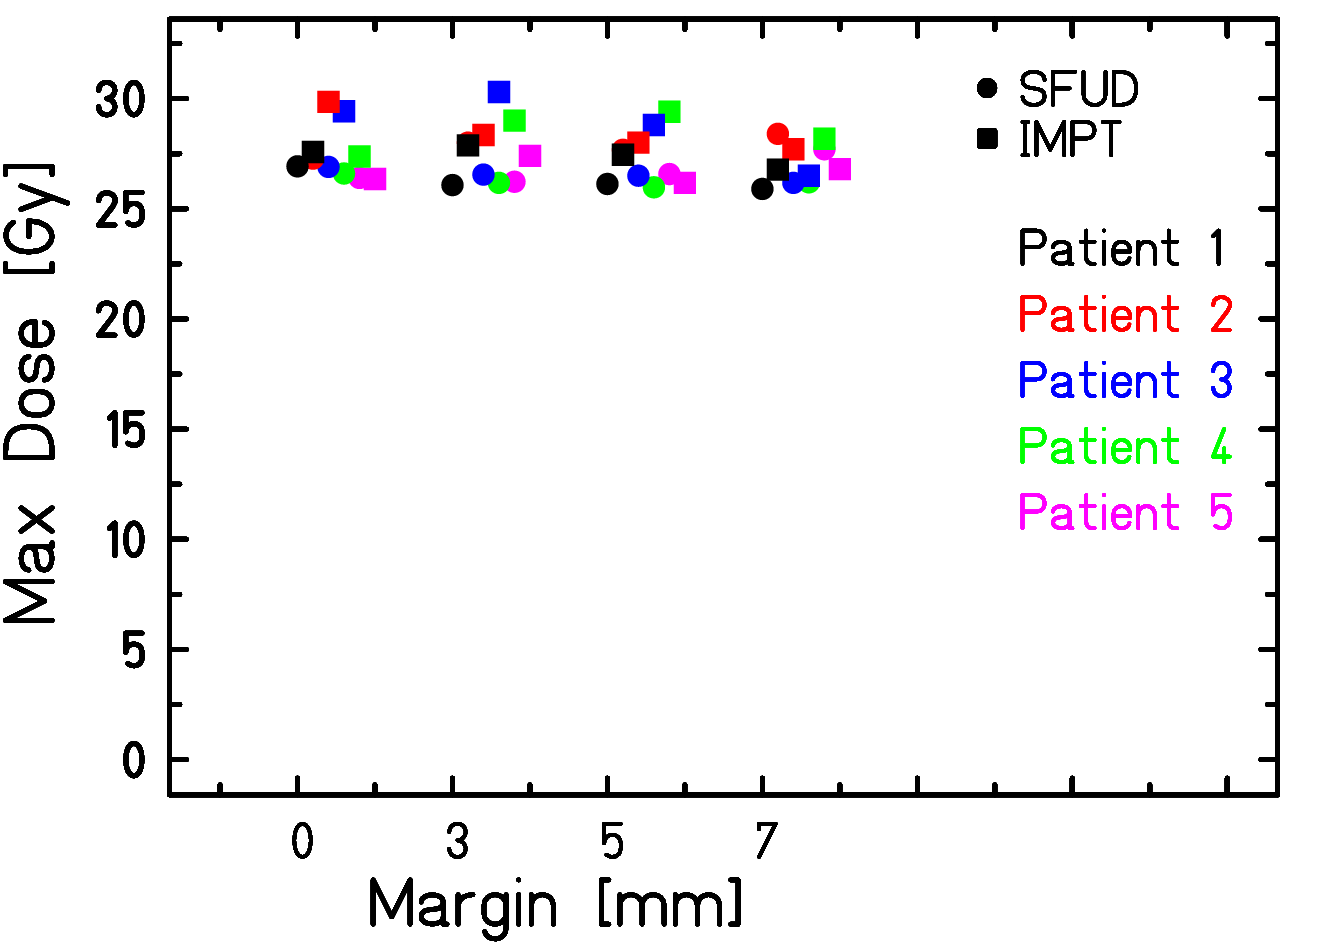
\includegraphics[scale=0.18]{Mayo_Human_HEARTwoOverlap_MaxDose.png}
 }
 
 \subfigure[Heart: maximum volume]{
 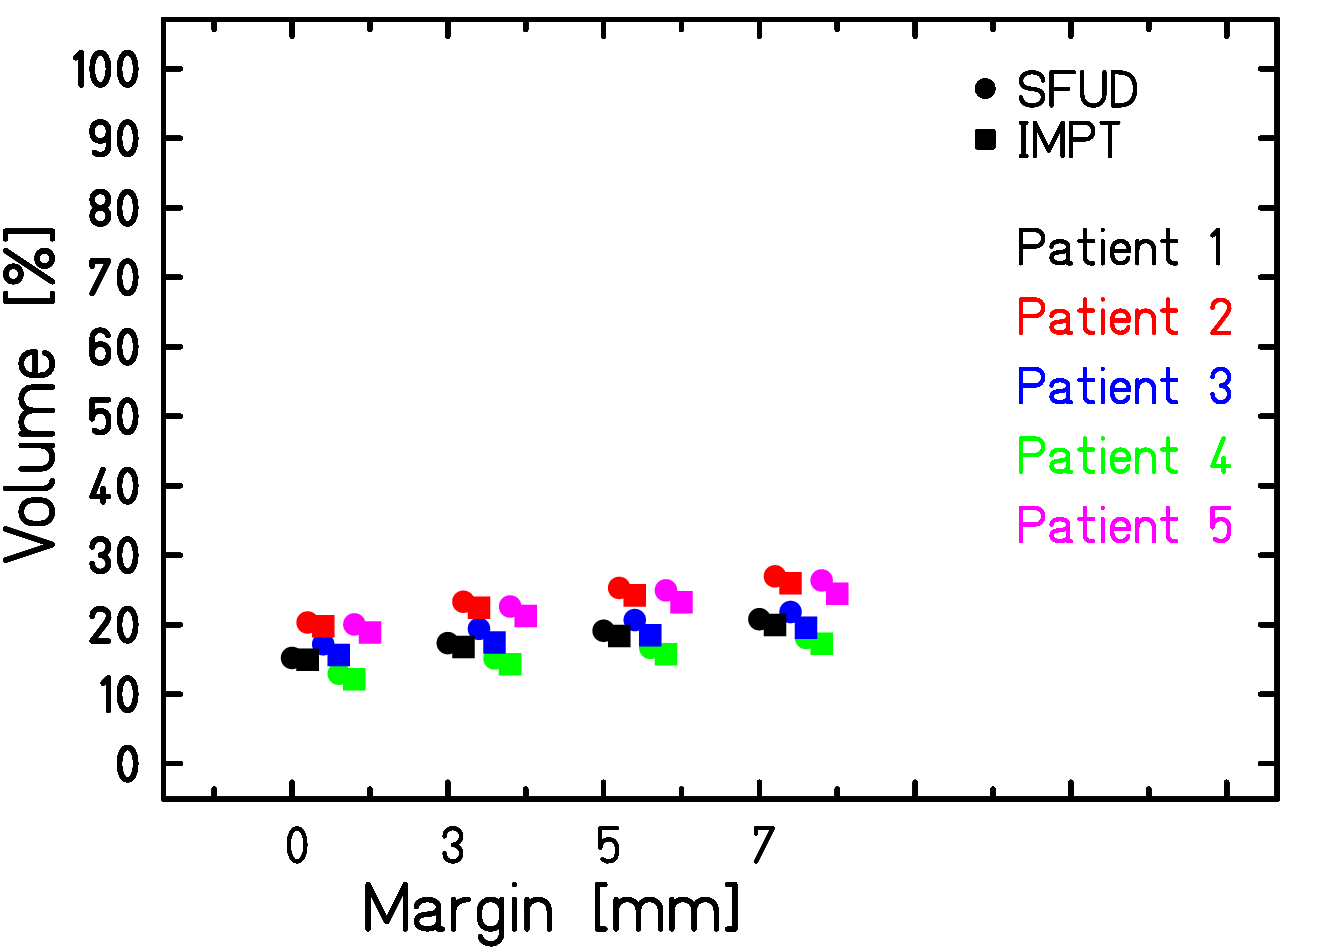
\includegraphics[scale=0.18]{Mayo_Human_HEARTwoOverlap_MaxVolume.png}
 }
\caption{Mean and maximum dose to the heart and maximal irradiated heart volume when irradiating the LPV and RPV in the five patient data sets with 
different margins (0 mm, 3 mm, 5 mm, 7mm) and two different delivery techniques (SFUD irradiation and IMPT).}
\label{static_margin_dose_heart}
\end{center}
\end{figure}

\newpage

%%%%%%%% DOSE TO THE VENTRICLES

The results for the analysis of the affected cardiac substructures can be found in figures \ref{static_margin_dose_ventricle} and 
\ref{static_margin_dose_coronary_arteries}.
Concerning the ventricles it can be seen that the mean dose is negligible (see figure \ref{static_margin_dose_ventricle}). 
% % For the LV the median results to 0.01Gy (75th percentile: 0.01Gy) with an SFUD irradiation compared to 
% % 0.01 Gy (75th percentile: 0.01 Gy) with IMPT for no added margin. With safety margins, the median is found to 0.02Gy 
% % (75th percentile: 0.02Gy) with SFUD versus 0.01Gy(75th percentile: 0.02Gy) with IMPT, 0.02Gy (75th percentile: 0.04Gy) versus 0.02Gy 
% % (75th percentile: 0.03Gy) and 0.03Gy (75th percentile: 0.05Gy) versus 
% % 0.03Gy (75th percentile: 0.04Gy) with 3mm, 5mm and 7mm, respectively. For the RV the median dose and third quartile all 
% % result to 0Gy for no margin and 3mm margin. For 5mm margin it is found to 0.01Gy(75th percentile: 0.01Gy) for SFUD as well as 
% % IMPT irradiation and for 7mm margin to 0.03Gy(75th percentile: 0.03Gy) for SFUD compared to 0.02Gy(75th percentile: 0.02Gy) for IMPT. 
The result for the maximal point dose is patient anatomy dependent. While patient 2 receives 
a higher LV maximal point dose than all the other patients (about 5Gy), no dose is deposited in the RV of this patient for any added margin. 
For an IMPT irradiation the median and 75th percentile of the maximal dose to the LV and RV over all patients and for all safety margin 
cases is shown in table \ref{tab:maxdose_ventricle}. For both ventricles the dose is increasing with the size of the safety margin. The left 
ventricle is receiving a higher maximum point dose than the right ventricle in all cases. Concerning the maximal irradiated volume 
it can also be stated that the LV is irradiated to a higher extend than the RV, and that also the affected volume is increasing with the 
underlying safety margin size (see table \ref{tab:maxvolume_ventricle}). 


% \vspace*{-1cm}

% \begin{table}[H]
%   \centering
%   \caption{Median maximum point dose to the ventricles.}
%   \begin{tabular}{|c|c|c|c|}
%     \hline\hline
%     Margin & Median LV [Gy] & 25th quartile LV [Gy] & 75th quartile LV [Gy] \\
%     \hline
%     0 mm & 0.93 & 0.62 & 1.30 \\
%     3 mm & 1.45 & 0.93 & 2.40 \\
%     5 mm & 1.80 & 1.20 & 4.47 \\
%     7 mm & 3.17 & 1.50 & 5.95 \\
%     \hline\hline
%     Margin & Median RV [Gy] & 25th quartile RV [Gy] & 75th quartile RV [Gy] \\
%     \hline
%     0 mm & 0.03 & 0.00 & 0.12 \\
%     3 mm & 0.88 & 0.00 & 1.33 \\
%     5 mm & 2.47 & 0.00 & 3.17 \\
%     7 mm & 4.12 & 0.00 & 4.80 \\
%     \hline\hline
%   \end{tabular}
%   \label{tab:maxdose_ventricle}
% \end{table}

\begin{table}[H]
  \centering
  \caption{Median and 75th percentile of maximum point dose to the ventricles.}
  \begin{tabular}{|c|c|c|}
    \hline\hline
    Margin & LV: Median (75th percentile) [Gy] & RV: Median (75th percentile) [Gy] \\
    \hline
    0 mm & 0.9 (1.3) & 0.0 (0.1) \\
    3 mm & 1.5 (2.4) & 0.9 (1.3) \\
    5 mm & 1.8 (4.5) & 2.5 (3.2) \\
    7 mm & 3.2 (6.0) & 4.1 (4.8) \\
    \hline\hline
%     Margin & RV: Median [Gy] & RV: 75th [Gy] \\
%     \hline
%     0 mm & 0.03 & 0.12 \\
%     3 mm & 0.88 & 1.33 \\
%     5 mm & 2.47 & 3.17 \\
%     7 mm & 4.12 & 4.80 \\
%     \hline\hline
  \end{tabular}
  \label{tab:maxdose_ventricle}
\end{table}

% \vspace*{-0.3cm}

\begin{table}[H]
  \centering
  \caption{Median and 75th percentile of maximum irradiated volume of ventricles.}
  \begin{tabular}{|c|c|c|}
    \hline\hline
    Margin & LV: Median (75th percentile) [\%] & RV: Median (75th percentile) [\%]\\
    \hline
    0 mm & 4.7 (5.1) & 0.00 (0.1) \\
    3 mm & 6.1 (7.3) & 0.5 (0.6) \\
    5 mm & 7.3 (9.1) & 1.1 (1.2) \\
    7 mm & 8.9 (10.8) & 1.8 (2.1) \\
    \hline\hline
%     Margin & RV: Median [\%] & RV: 75th [\%] \\
%     \hline
%     0 mm & 0.01 & 0.08 \\
%     3 mm & 0.52 & 0.62 \\
%     5 mm & 1.05 & 1.19 \\
%     7 mm & 1.81 & 2.14 \\
%     \hline\hline
  \end{tabular}
  \label{tab:maxvolume_ventricle}
\end{table}


% \begin{table}[H]
%   \centering
%   \caption{Median maximum irradiated volume of ventricles.}
%   \begin{tabular}{|c|c|c|c|}
%     \hline\hline
%     Margin & Median LV [\%] & 25th quartile LV [\%] & 75th quartile LV [\%] \\
%     \hline
%     0 mm & 4.65 & 1.60 & 5.14 \\
%     3 mm & 6.08 & 2.60 & 7.32 \\
%     5 mm & 7.31 & 3.52 & 9.12 \\
%     7 mm & 8.86 & 4.52 & 10.72 \\
%     \hline\hline
%     Margin & Median RV [\%] & 25th quartile RV [\%] & 75th quartile RV [\%] \\
%     \hline
%     0 mm & 0.01 & 0.00 & 0.08 \\
%     3 mm & 0.52 & 0.00 & 0.62 \\
%     5 mm & 1.05 & 0.00 & 1.19 \\
%     7 mm & 1.81 & 0.00 & 2.14 \\
%     \hline\hline
%   \end{tabular}
%   \label{tab:maxvolume_ventricle}
% \end{table}


%%%%%%%% DOSE TO THE VENTRICLES

\newpage

\begin{figure}[H]
\subfigure[Mean dose: LV]{
 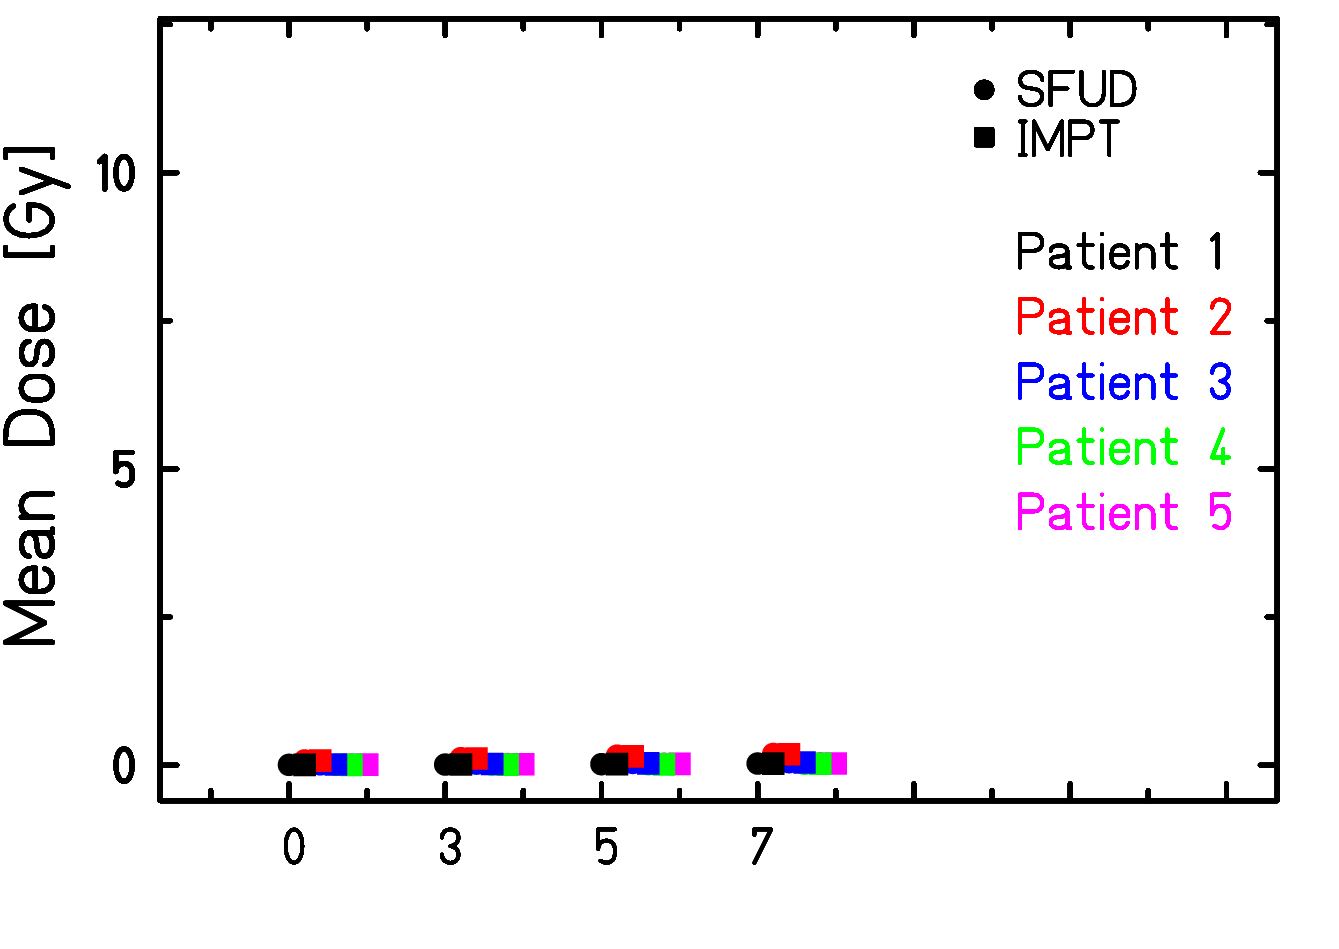
\includegraphics[scale=0.18]{Mayo_Human_LV_MeanDose.png}
 }
 \subfigure[Mean dose: RV]{
 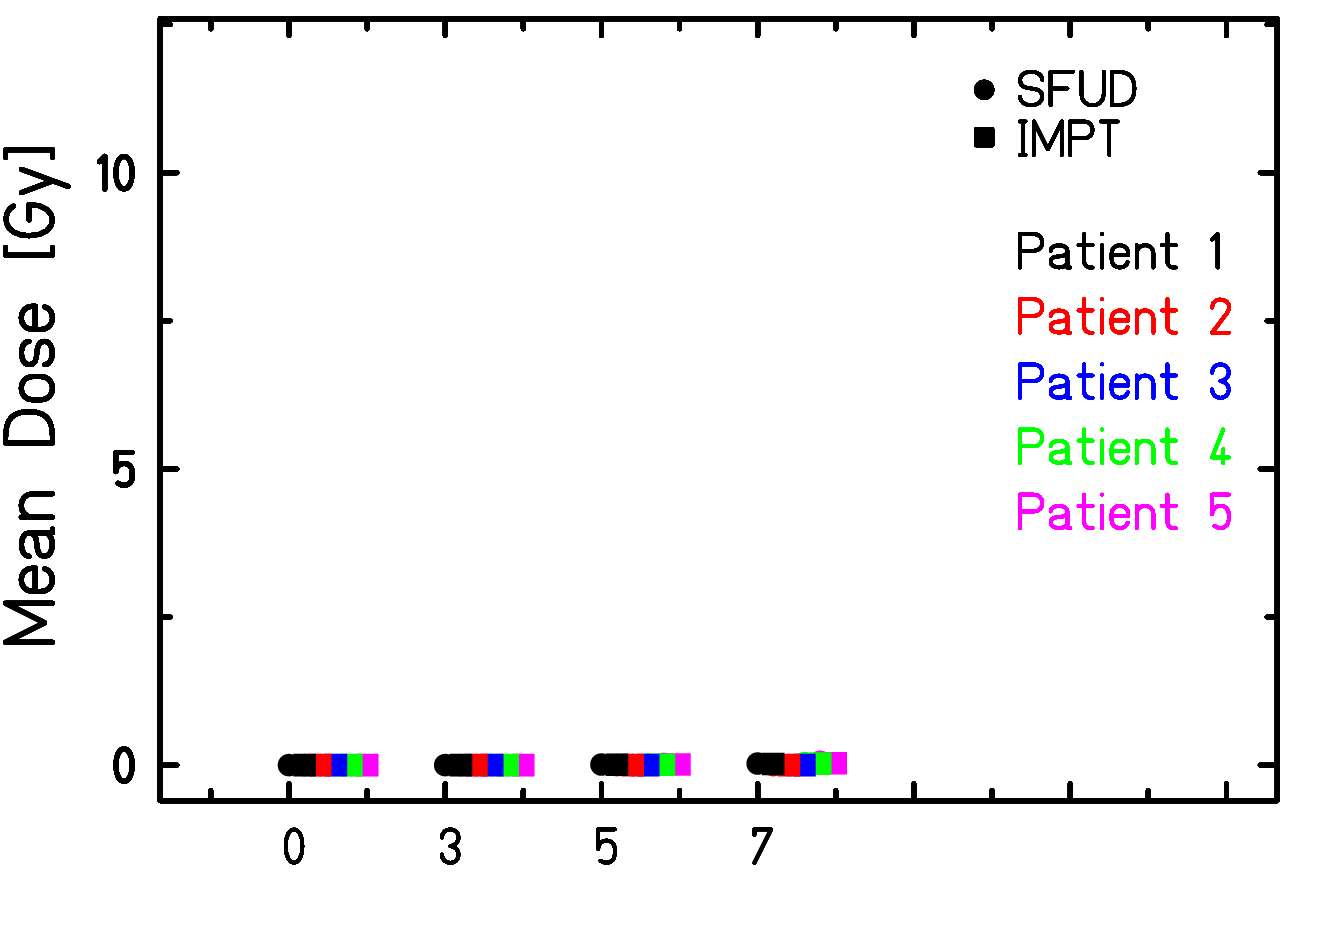
\includegraphics[scale=0.18]{Mayo_Human_RV_MeanDose.png}
 }
 \subfigure[Maximum point dose: LV]{
 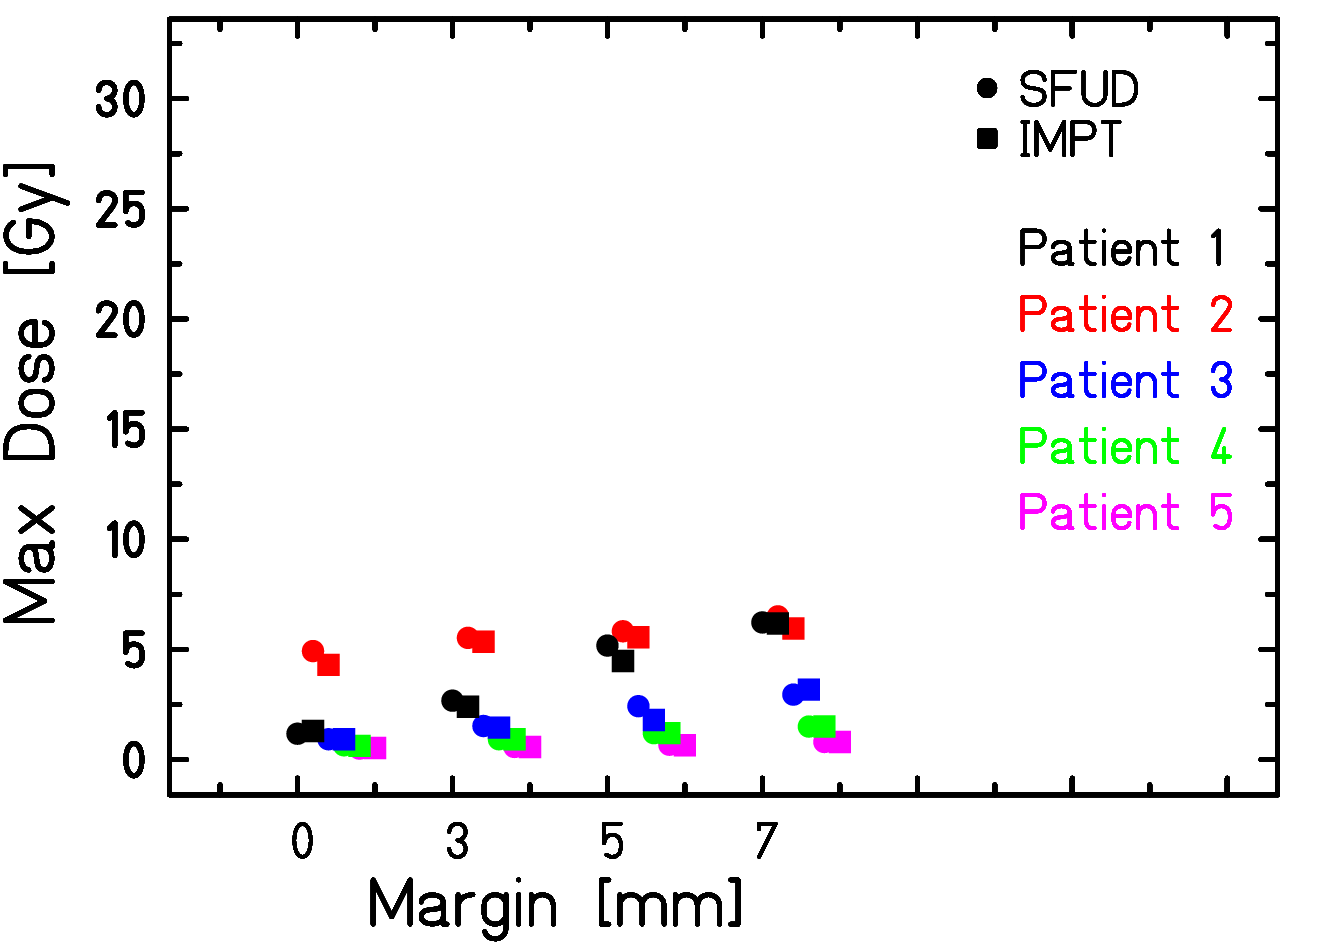
\includegraphics[scale=0.18]{Mayo_Human_LV_MaxDose.png}
 }
 \subfigure[Maximum point dose: RV]{
 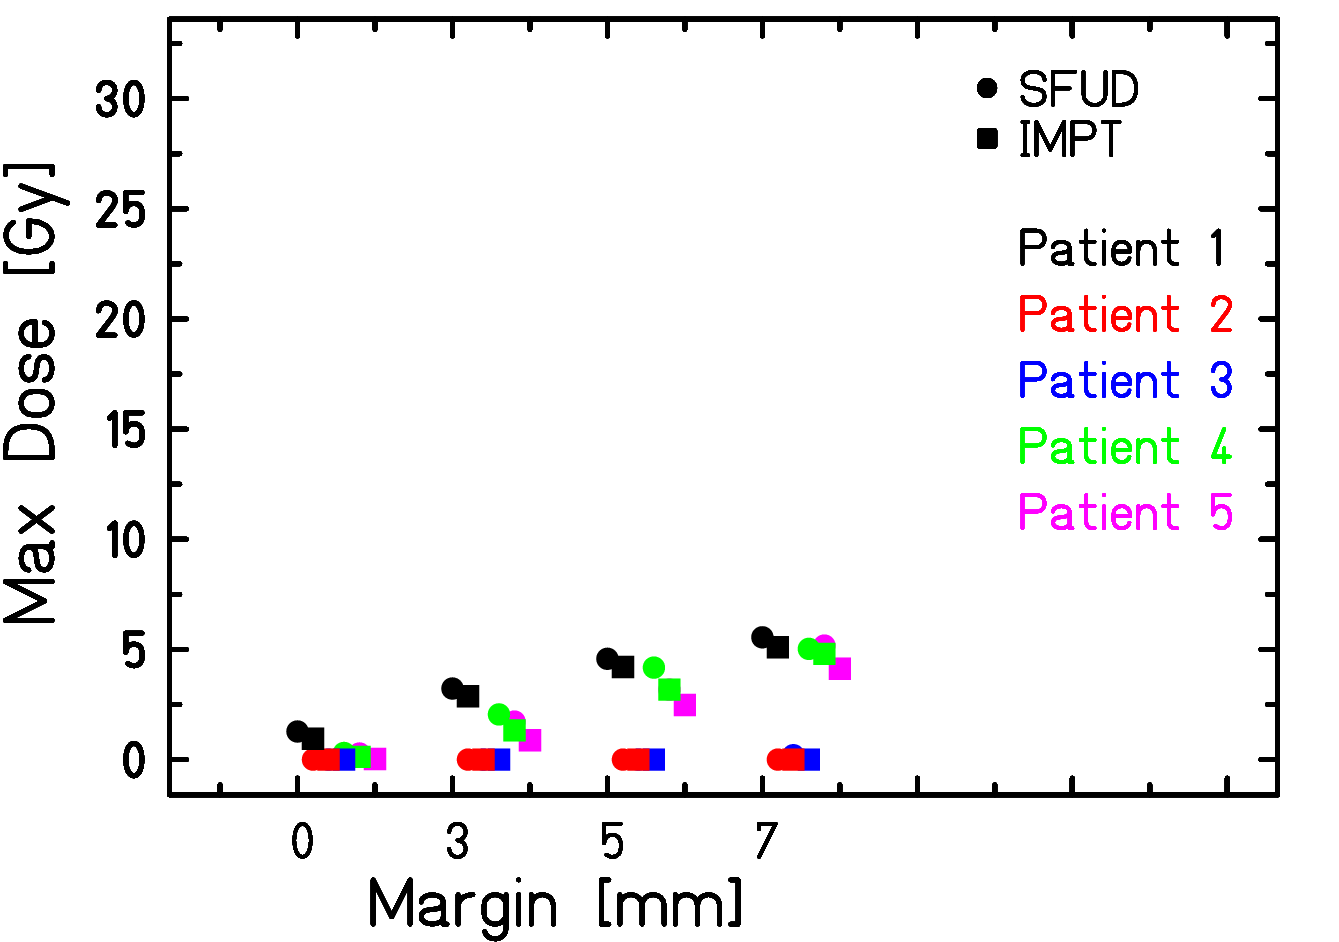
\includegraphics[scale=0.18]{Mayo_Human_RV_MaxDose.png}
 }
 \subfigure[Maximum volume: LV]{
 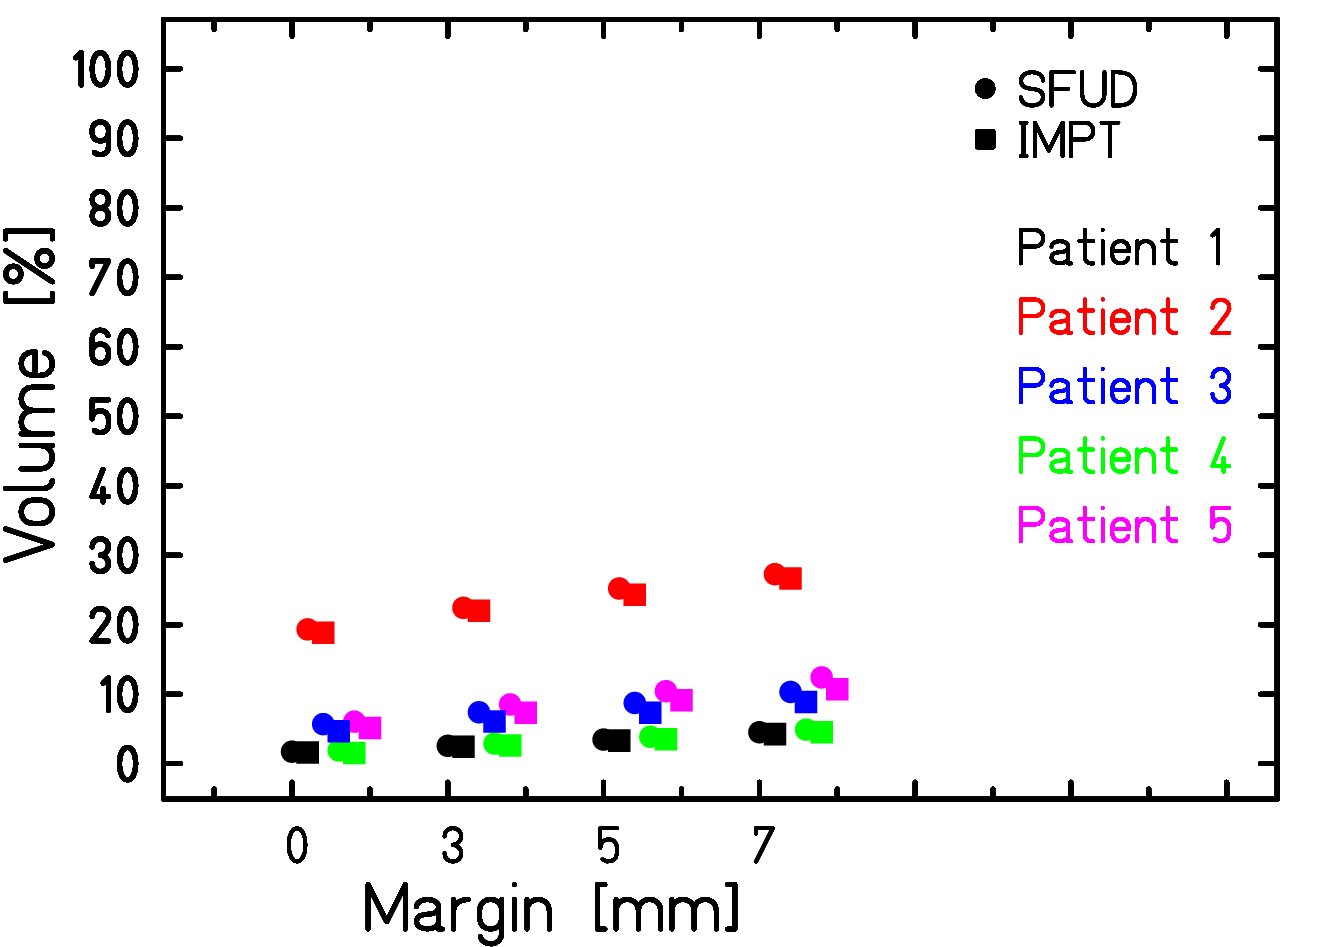
\includegraphics[scale=0.18]{Mayo_Human_LV_MaxVolume.png}
 }
 \subfigure[Maximum volume: RV]{
 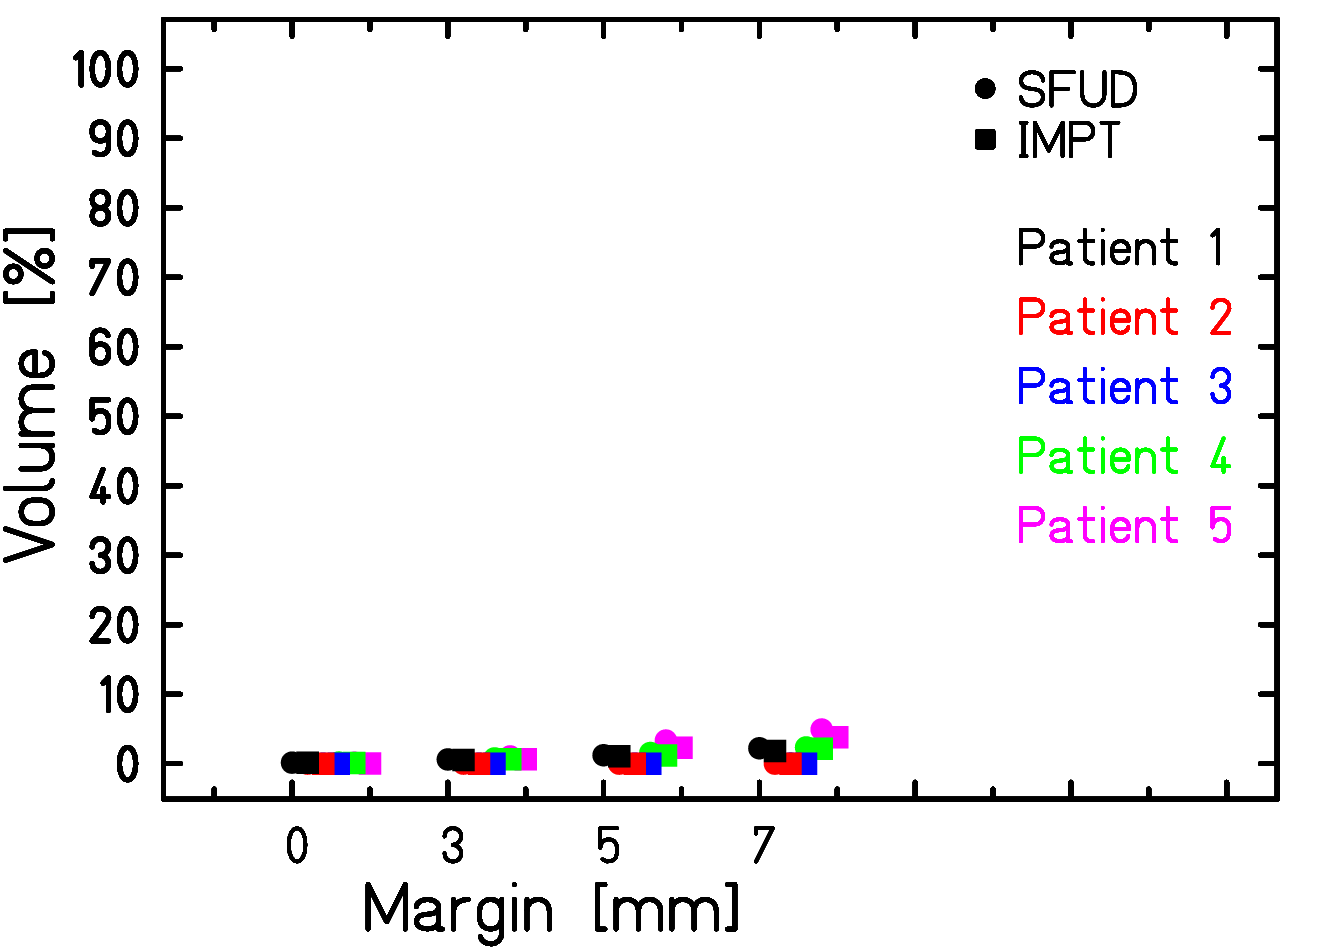
\includegraphics[scale=0.18]{Mayo_Human_RV_MaxVolume.png}
 }
\caption{Mean dose, maximal point dose and maximal irradiated volume of left ventricle (LV) and right ventricle (RV), respectively, when irradiating the LPV 
and RPV in the five patient data sets with different margins (0 mm, 3 mm, 5 mm, 7mm) and two different delivery techniques (SFUD irradiation and IMPT).}
\label{static_margin_dose_ventricle}
\end{figure}

%%%%%%%% DOSE TO THE CA

Concerning the coronary arteries, it can be seen that the LCA and RCA are receiving a comparable mean dose. The maximum point dose on the other 
hand is higher for the LCA. The same is valid for the maximum irradiated volume. This is due to the proximity of the upper LCA branches 
to the LPV target site. Due to the small vessel size of the coronary arteries this also results in a relatively high 
maximal irradiated volume. 
% Nevertheless, a median dose of less than 1Gy in most studied cases yields good results compared to the data 
% known from heart irradiation with photons (see Discussion XXX). 


\vspace*{-0.4cm}

\begin{table}[H]
  \centering
  \caption{Median and 75th percentile of mean dose to the coronary arteries.}
  \begin{tabular}{|c|c|c|}
    \hline\hline
    Margin & LCA: median (75th percentile) [Gy] & RCA: median (75th percentile) [Gy] \\
    \hline
    0 mm & 0.2 (0.5) & 0.3 (0.4) \\
    3 mm & 0.5 (0.9) & 0.5 (0.8) \\
    5 mm & 0.7 (1.1) & 0.7 (1.3) \\
    7 mm & 1.5 (1.6) & 1.0 (1.7) \\
    \hline\hline
%     Margin & RCA: median [Gy] & RCA: 75th [Gy] \\
%     \hline
%     0 mm & 0.28 & 0.36 \\
%     3 mm & 0.51 & 0.84 \\
%     5 mm & 0.72 & 1.30 \\
%     7 mm & 0.98 & 1.72 \\
%     \hline\hline
  \end{tabular}
  \label{tab:meandose_ca}
\end{table}

% \vspace*{-0.8cm}

\begin{table}[H]
  \centering
  \caption{Median and 75th percentile of maximum point dose to the coronary arteries.}
  \begin{tabular}{|c|c|c|}
    \hline\hline
    Margin & LCA: median (75th percentile) [Gy] & RCA: median (75th percentile) [Gy] \\
    \hline
    0 mm & 6.0 (6.3) & 3.1 (4.7) \\
    3 mm & 7.4 (7.6) & 3.8 (6.5) \\
    5 mm & 8.7 (13.2) & 4.3 (7.2) \\
    7 mm & 20.1 (21.3) & 5.9 (7.9) \\
    \hline\hline
%     Margin & RCA: median [Gy] & RCA: 75th [Gy] \\
%     \hline
%     0 mm & 3.08 & 4.70 \\
%     3 mm & 3.83 & 6.45 \\
%     5 mm & 4.25 & 7.22 \\
%     7 mm & 5.85 & 7.90 \\
%     \hline\hline
  \end{tabular}
  \label{tab:maxdose_ca}
\end{table}

% \vspace*{-0.8cm}

\begin{table}[H]
  \centering
  \caption{Median and 75th percentile of maximum irradiated volume of coronary arteries.}
  \begin{tabular}{|c|c|c|}
    \hline\hline
    Margin & LCA: median (75th percentile) [\%] & RCA: median (75th percentile) [\%] \\
    \hline
    0 mm & 26.7 (39.2) & 19.2 (26.5) \\
    3 mm & 28.5 (41.5) & 25.1 (29.8) \\
    5 mm & 29.6 (44.6) & 33.2 (35.6) \\
    7 mm & 31.4 (49.6) & 39.6 (39.7) \\
    \hline\hline
%     Margin & RCA: Median [\%] & RCA: 75th [\%] \\
%     \hline
%     0 mm & 19.24 & 26.48 \\
%     3 mm & 25.09 & 29.80 \\
%     5 mm & 33.21 & 35.57 \\
%     7 mm & 39.58 & 39.69 \\
%     \hline\hline
  \end{tabular}
  \label{tab:maxvolume_ventricle}
\end{table}


\newpage
%%%%%%%% DOSE TO THE CA

\begin{figure}[H]
\subfigure[Mean dose: LCA]{
 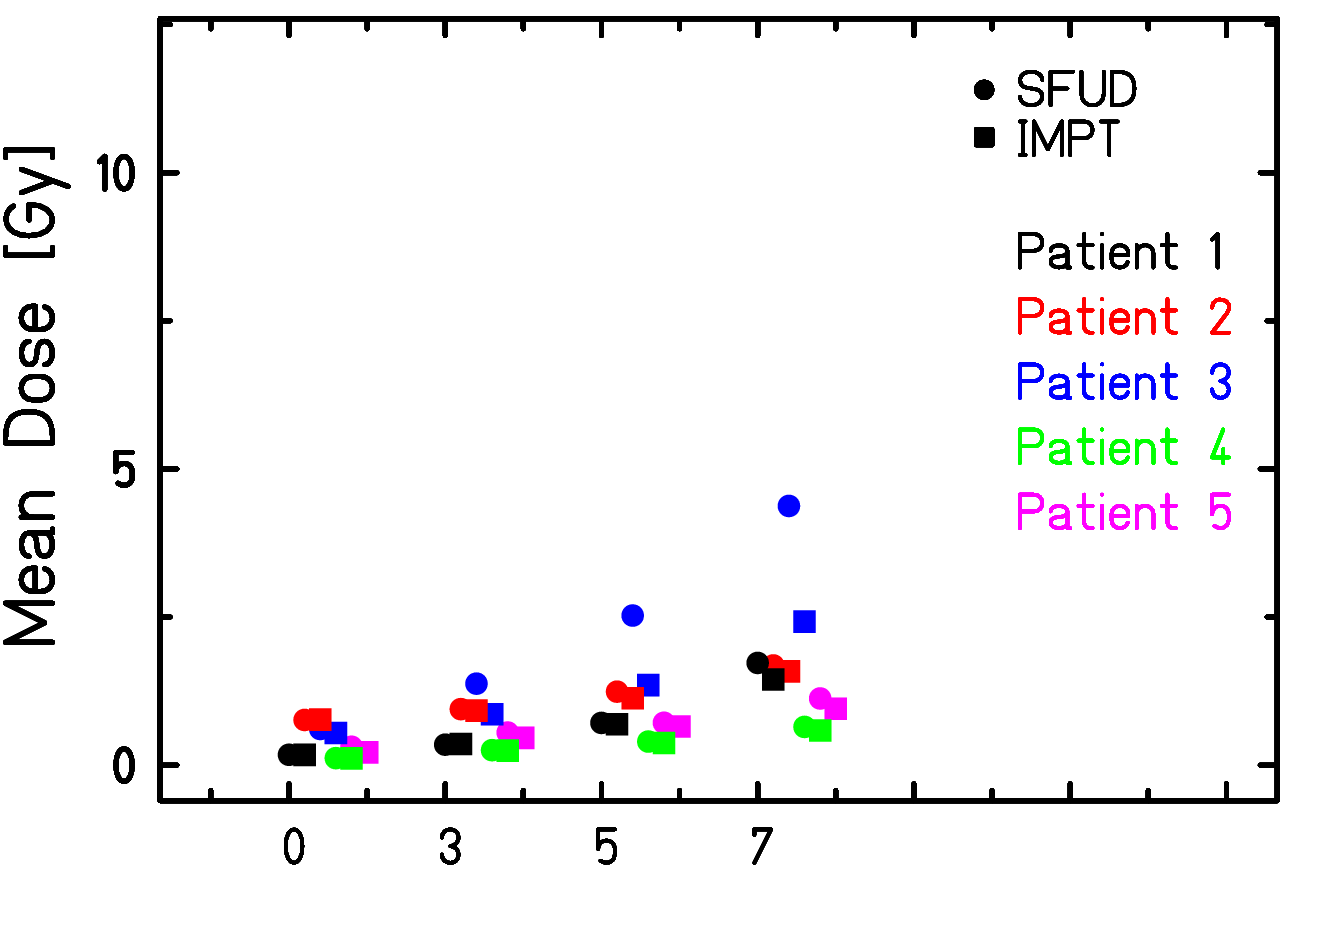
\includegraphics[scale=0.18]{Mayo_Human_LCA_MeanDose.png}
 }
 \subfigure[Mean dose: RCA]{
 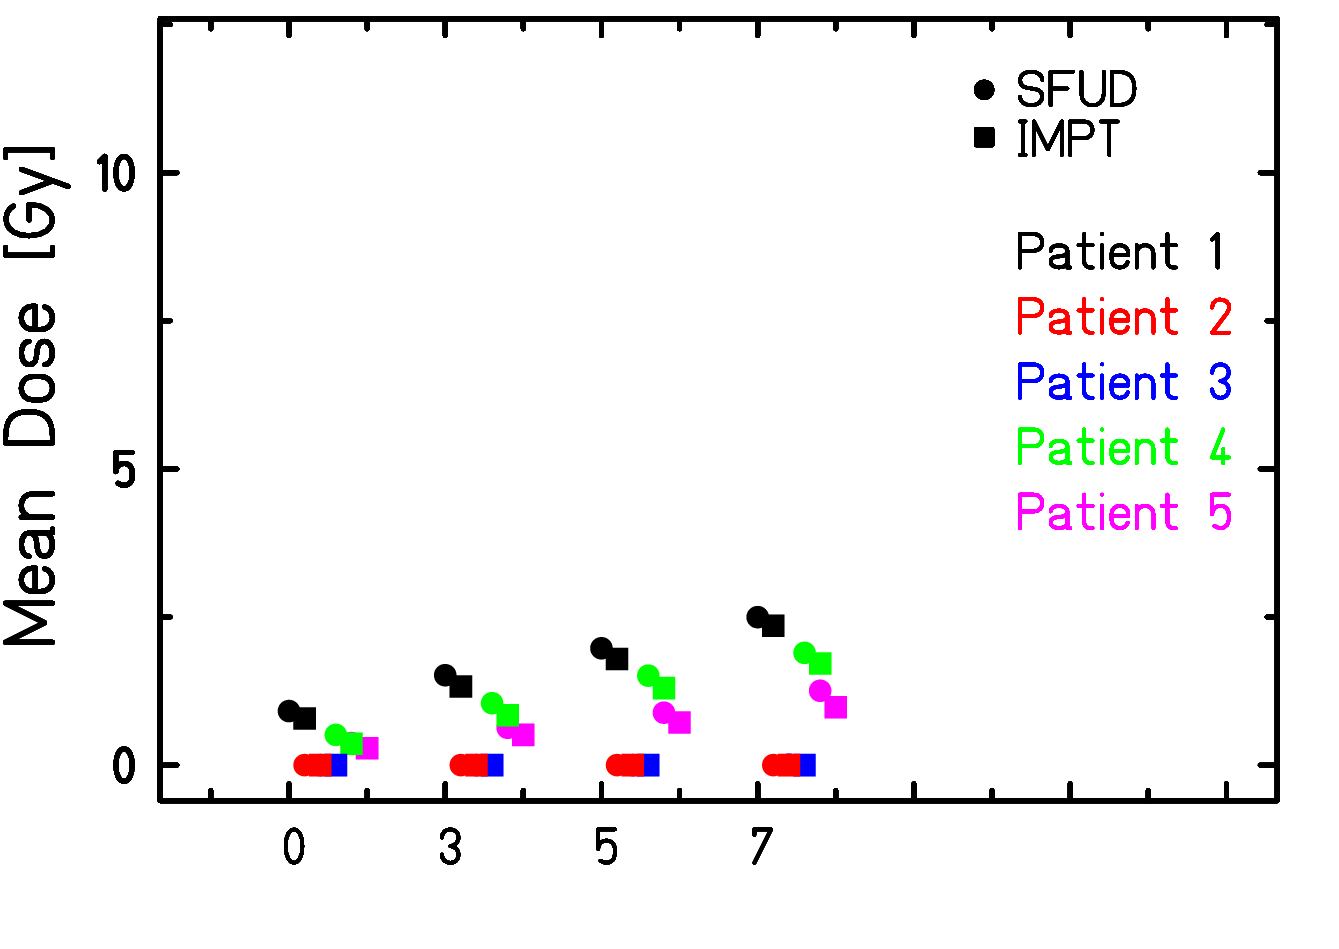
\includegraphics[scale=0.18]{Mayo_Human_RCA_MeanDose.png}
 }
 \subfigure[Maximum point dose: LCA]{
 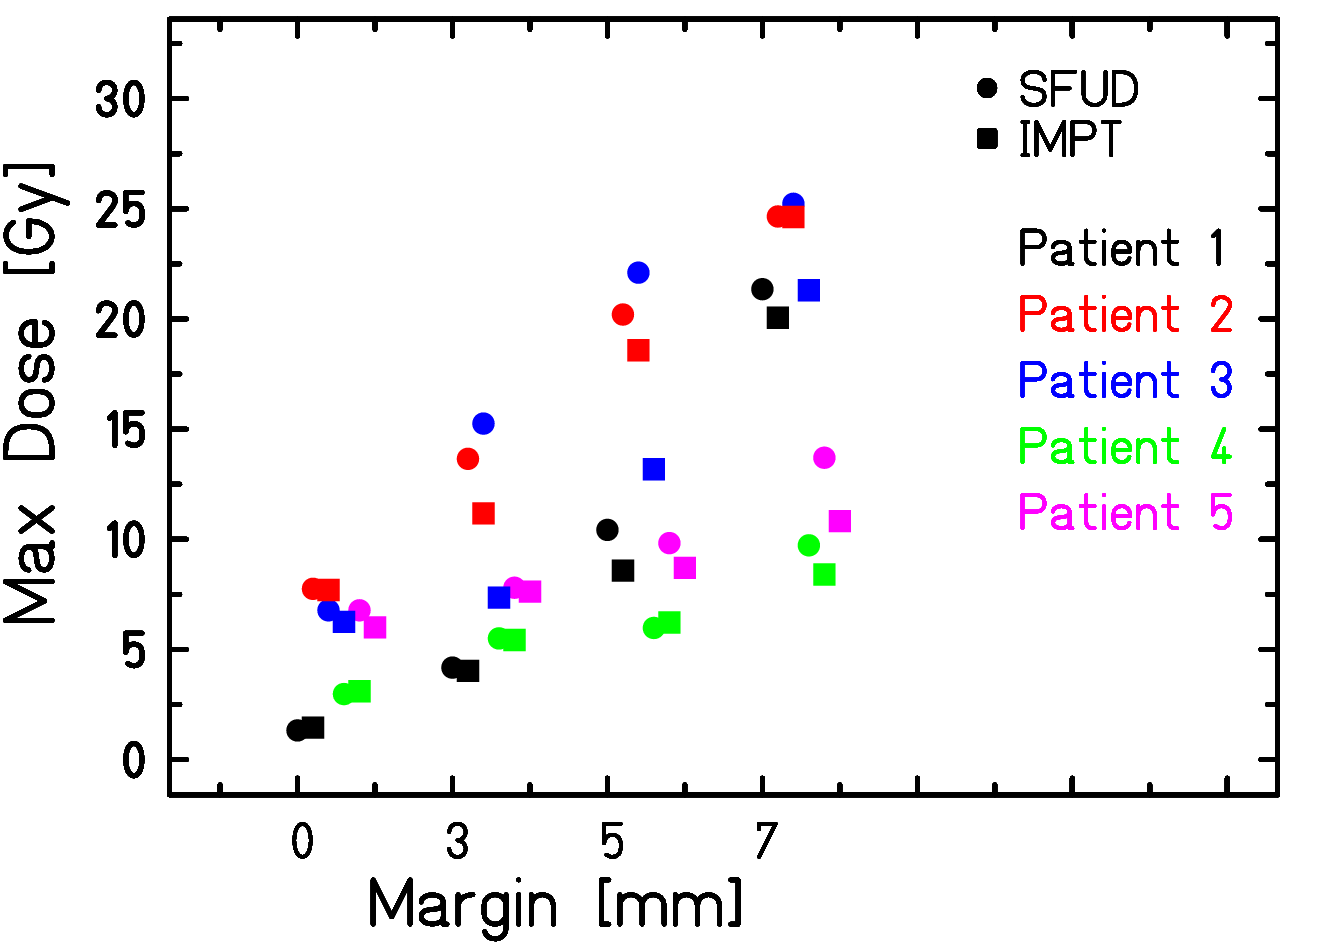
\includegraphics[scale=0.18]{Mayo_Human_LCA_MaxDose.png}
 }
 \subfigure[Maximum point dose: RCA]{
 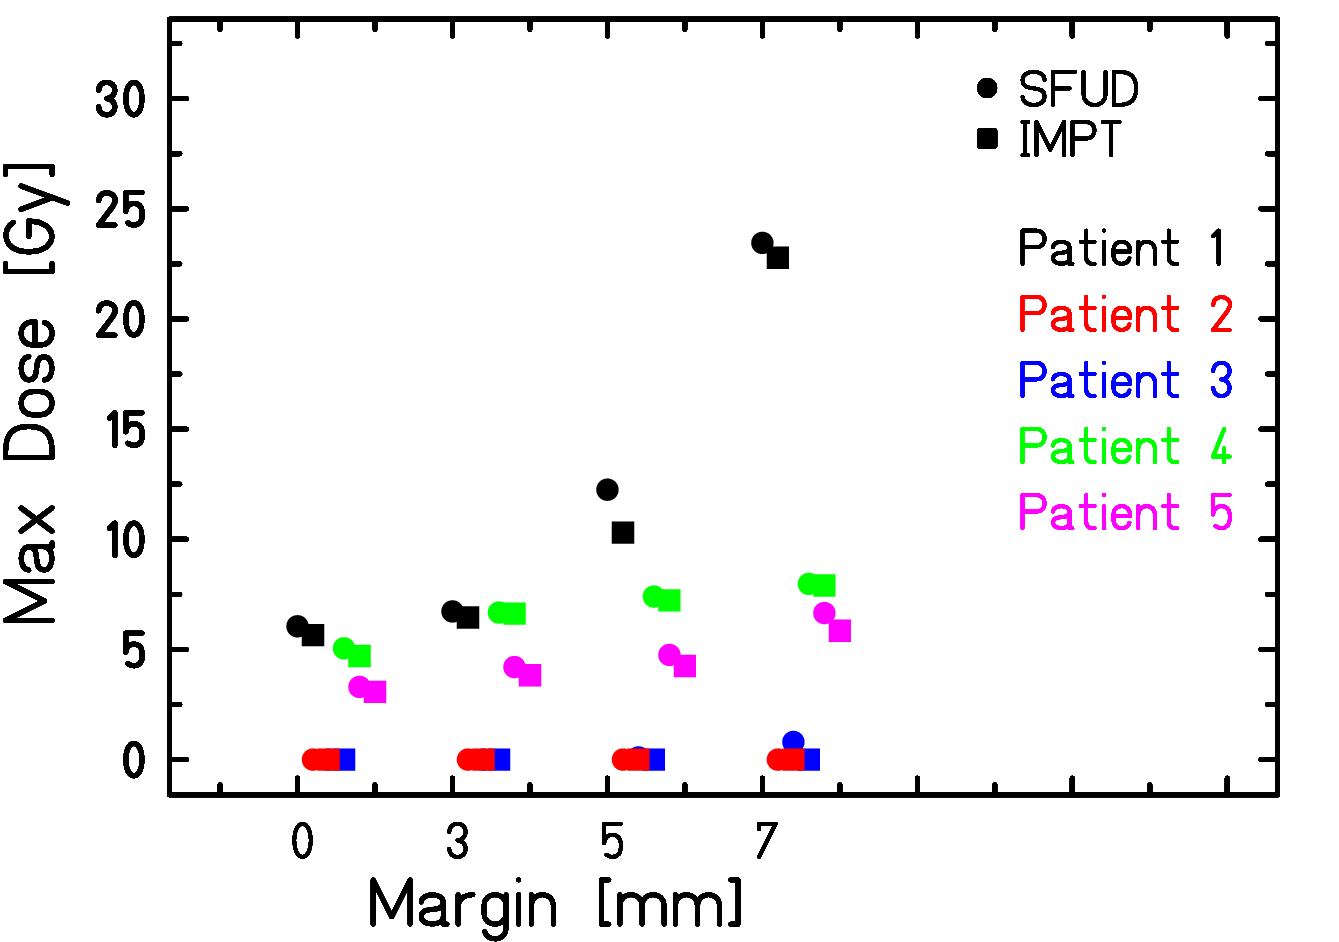
\includegraphics[scale=0.18]{Mayo_Human_RCA_MaxDose.png}
 }
 \subfigure[Maximum volume: LCA]{
 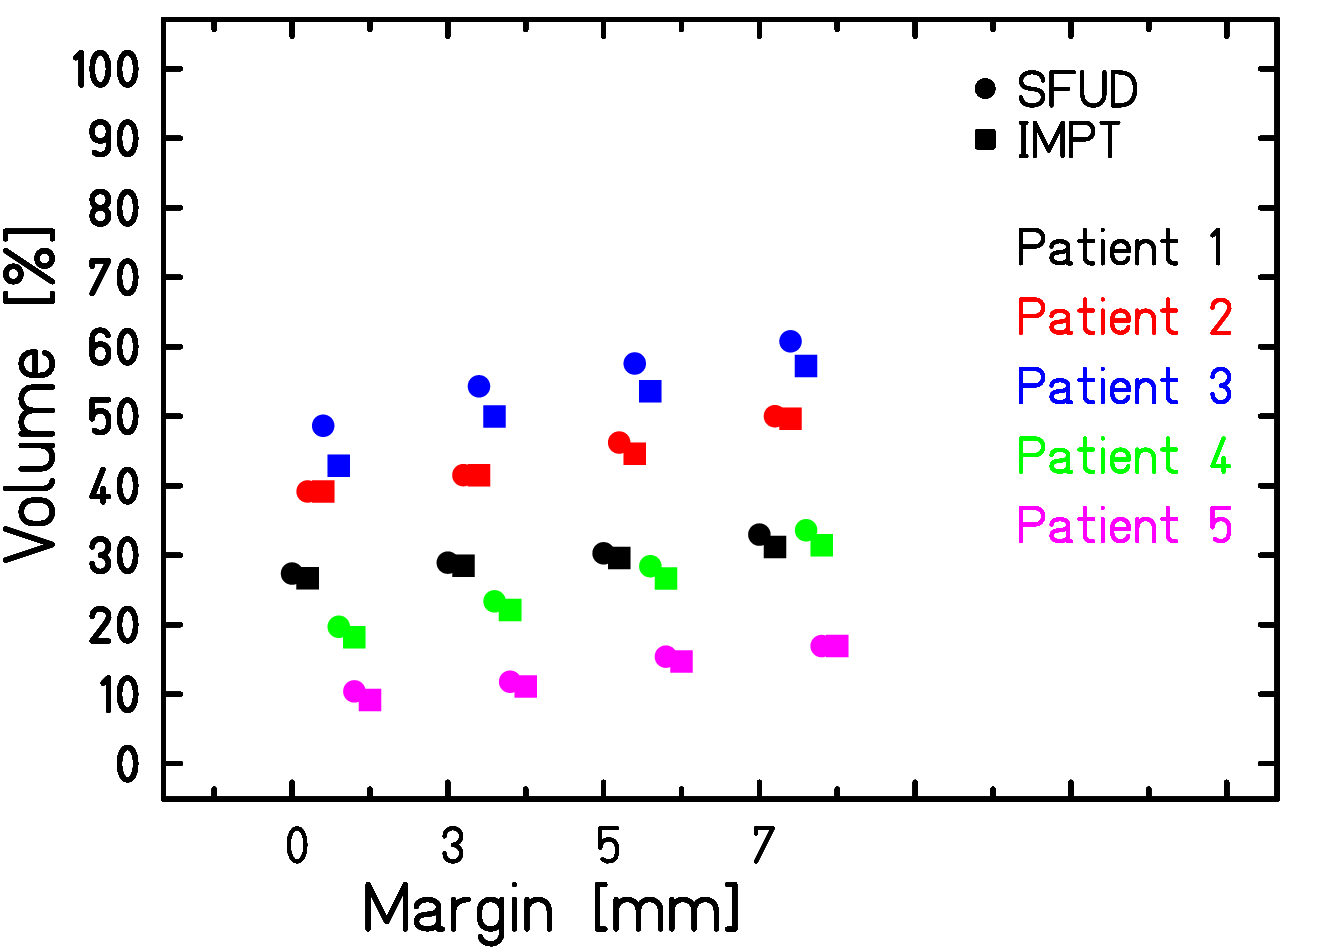
\includegraphics[scale=0.18]{Mayo_Human_LCA_MaxVolume.png}
 }
 \subfigure[Maximum volume: RCA]{
 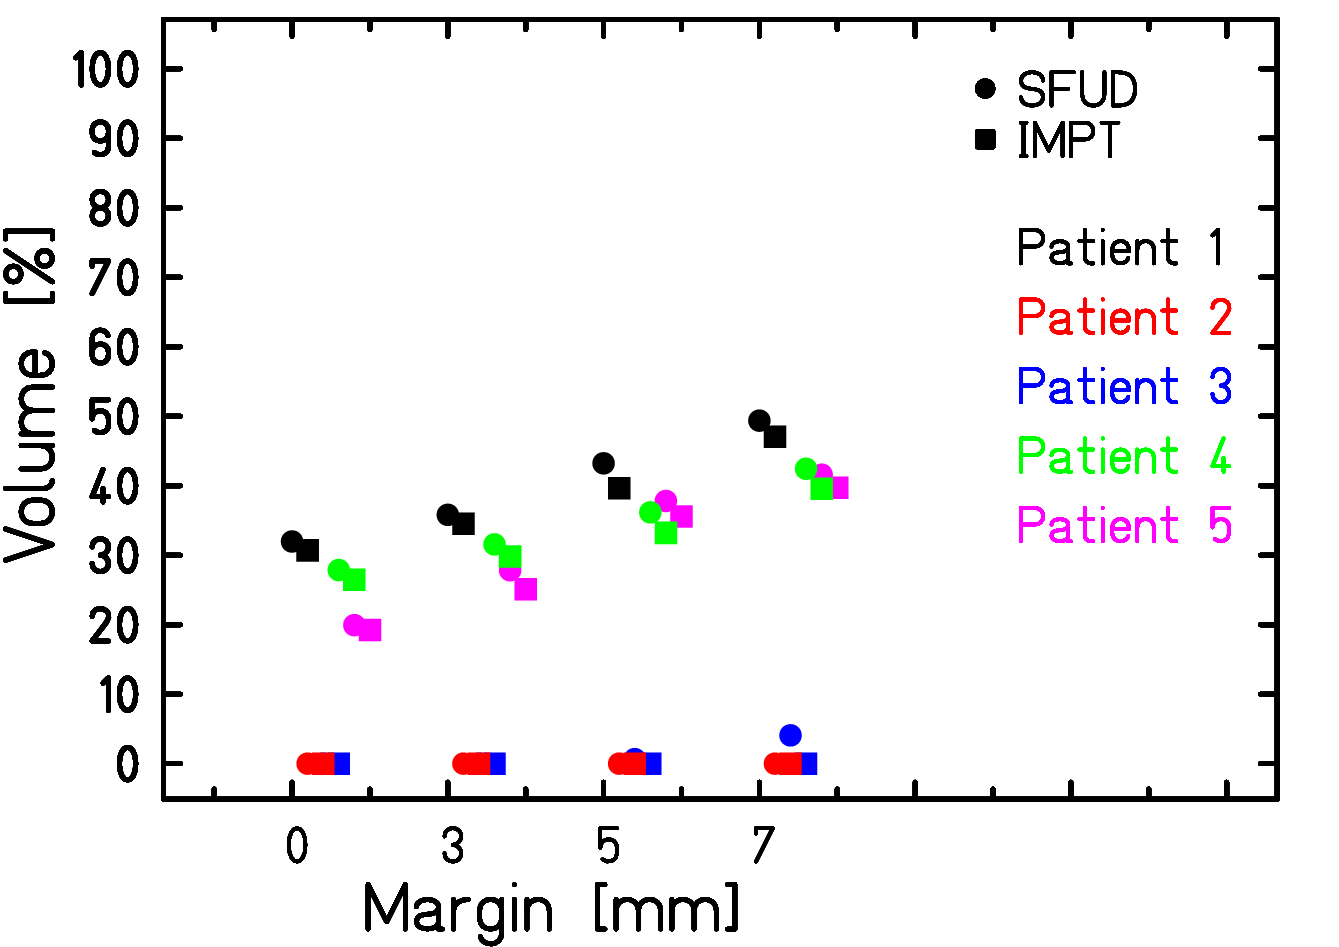
\includegraphics[scale=0.18]{Mayo_Human_RCA_MaxVolume.png}
 }
\caption{Mean dose, maximal point dose and maximal irradiated volume of left coronary artery (LCA) and right coronary artery (RCA), respectively, 
when irradiating the LPV and RPV in the five patient data sets with different margins (0 mm, 3 mm, 5 mm, 7mm) and two different delivery 
techniques (SFUD irradiation and IMPT).}
\label{static_margin_dose_coronary_arteries}
\end{figure}

% \begin{figure}[H]
% \subfigure[Mean dose: LA]{
%  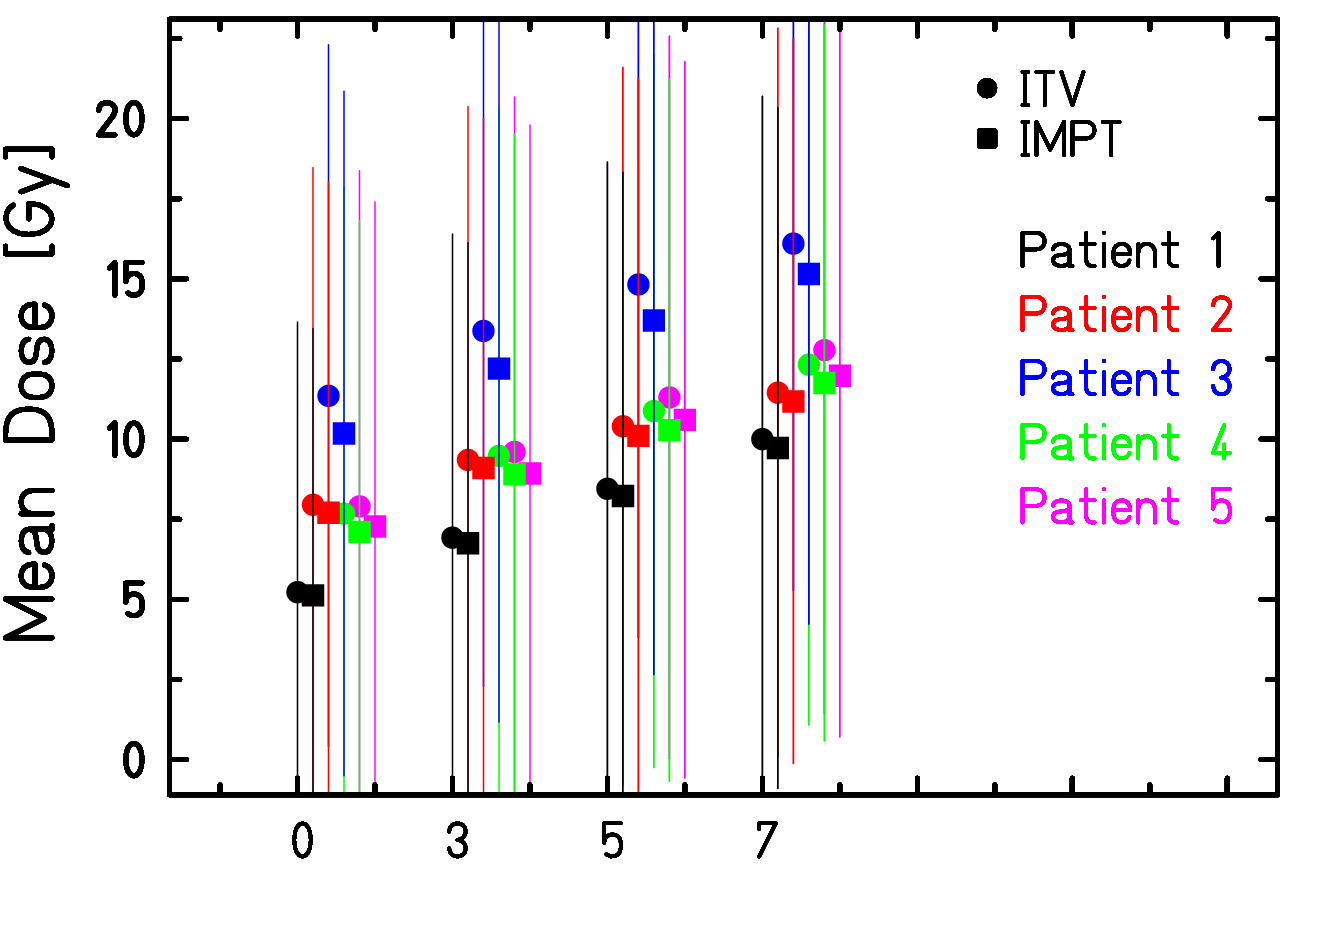
\includegraphics[scale=0.18]{Mayo_Human_LA_MeanDose.png}
%  }
%  \subfigure[Mean dose: RA]{
%  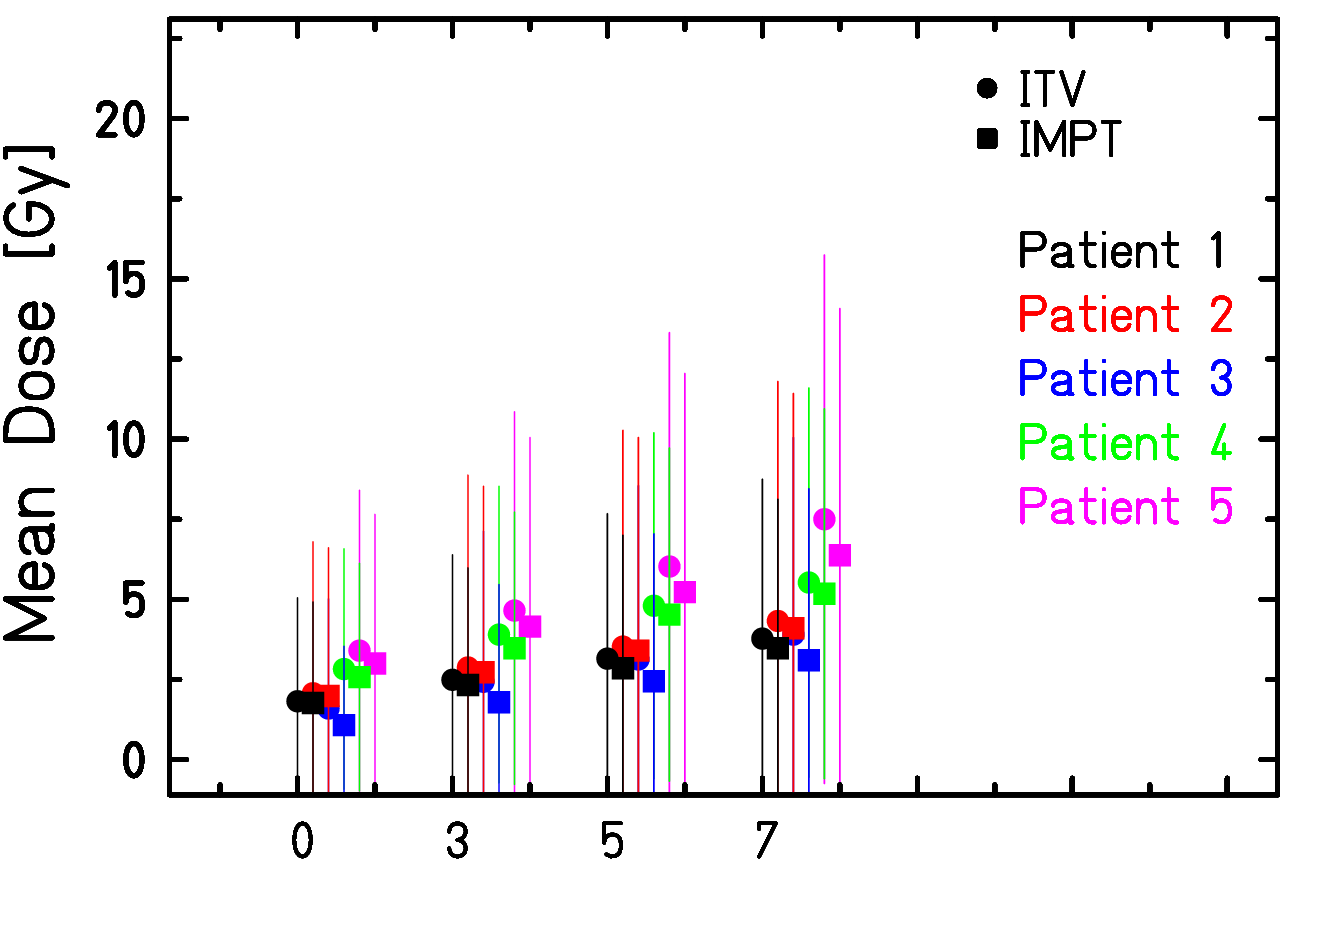
\includegraphics[scale=0.18]{Mayo_Human_RA_MeanDose.png}
%  }
%  \subfigure[Maximum point dose: LA]{
%  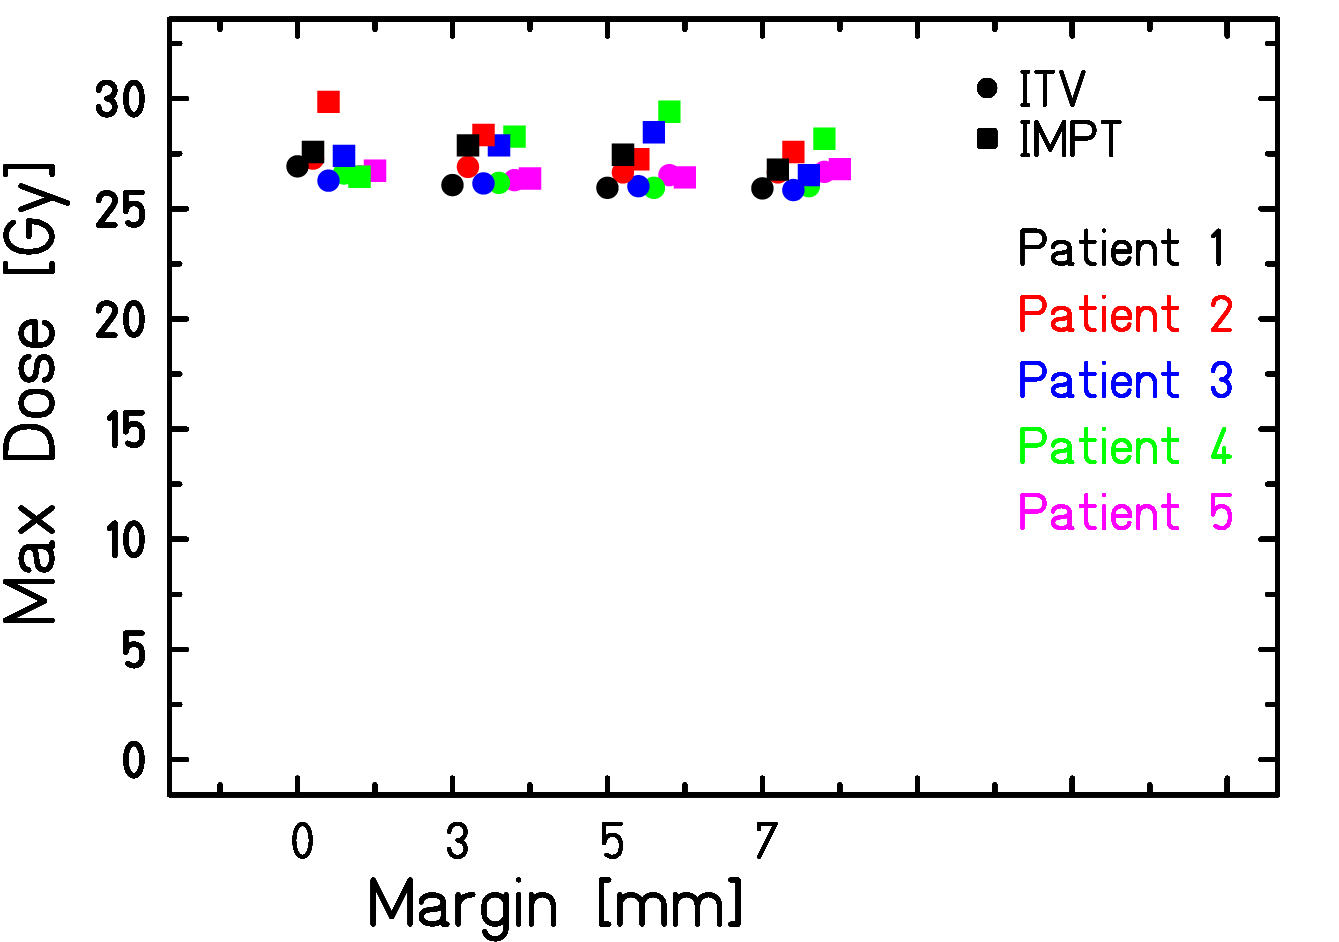
\includegraphics[scale=0.18]{Mayo_Human_LA_MaxDose.png}
%  }
%  \subfigure[Maximum point dose: RA]{
%  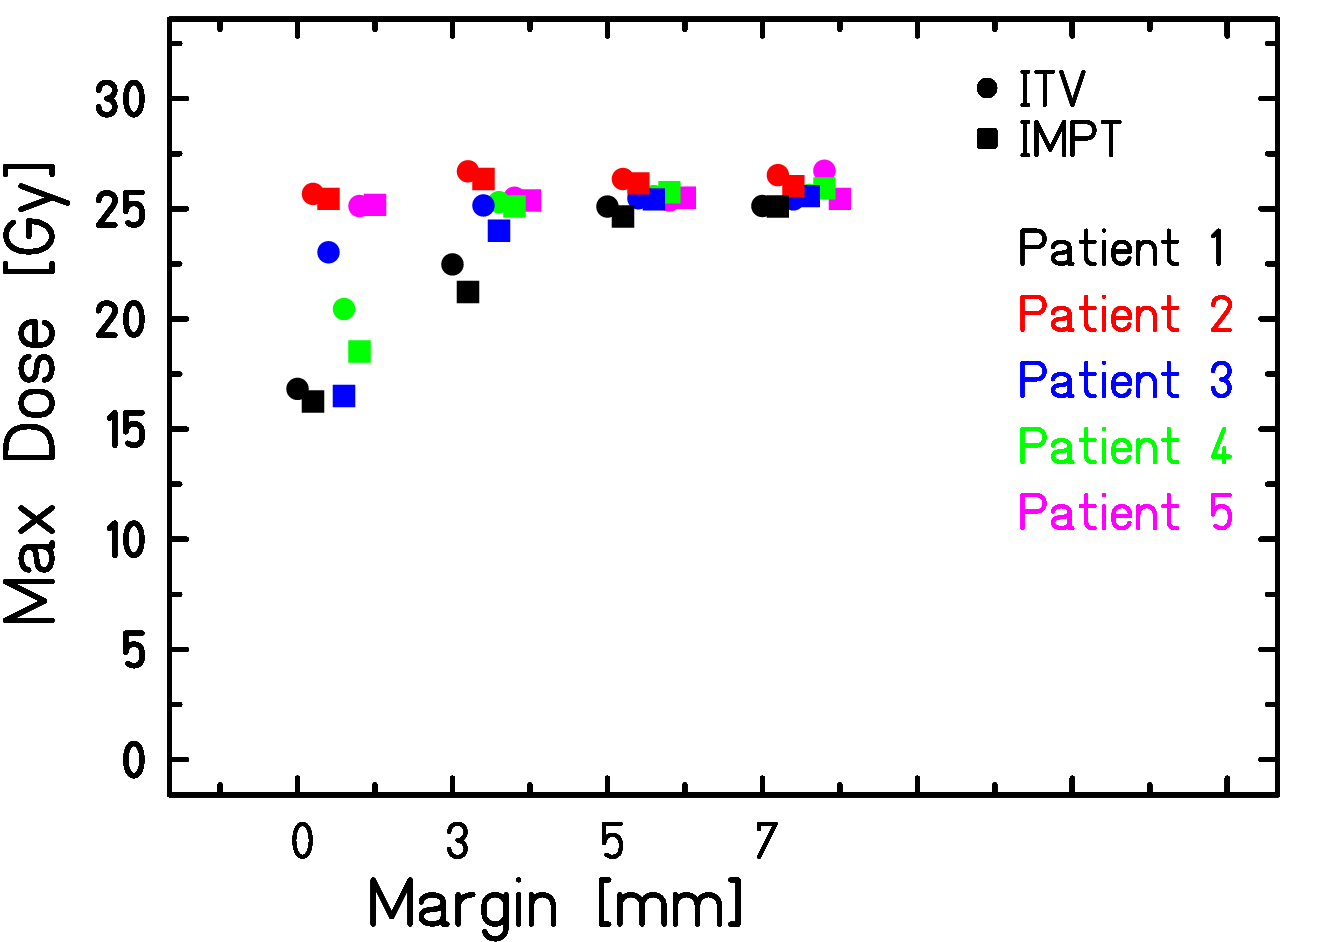
\includegraphics[scale=0.18]{Mayo_Human_RA_MaxDose.png}
%  }
%  \subfigure[Maximum volume: LA]{
%  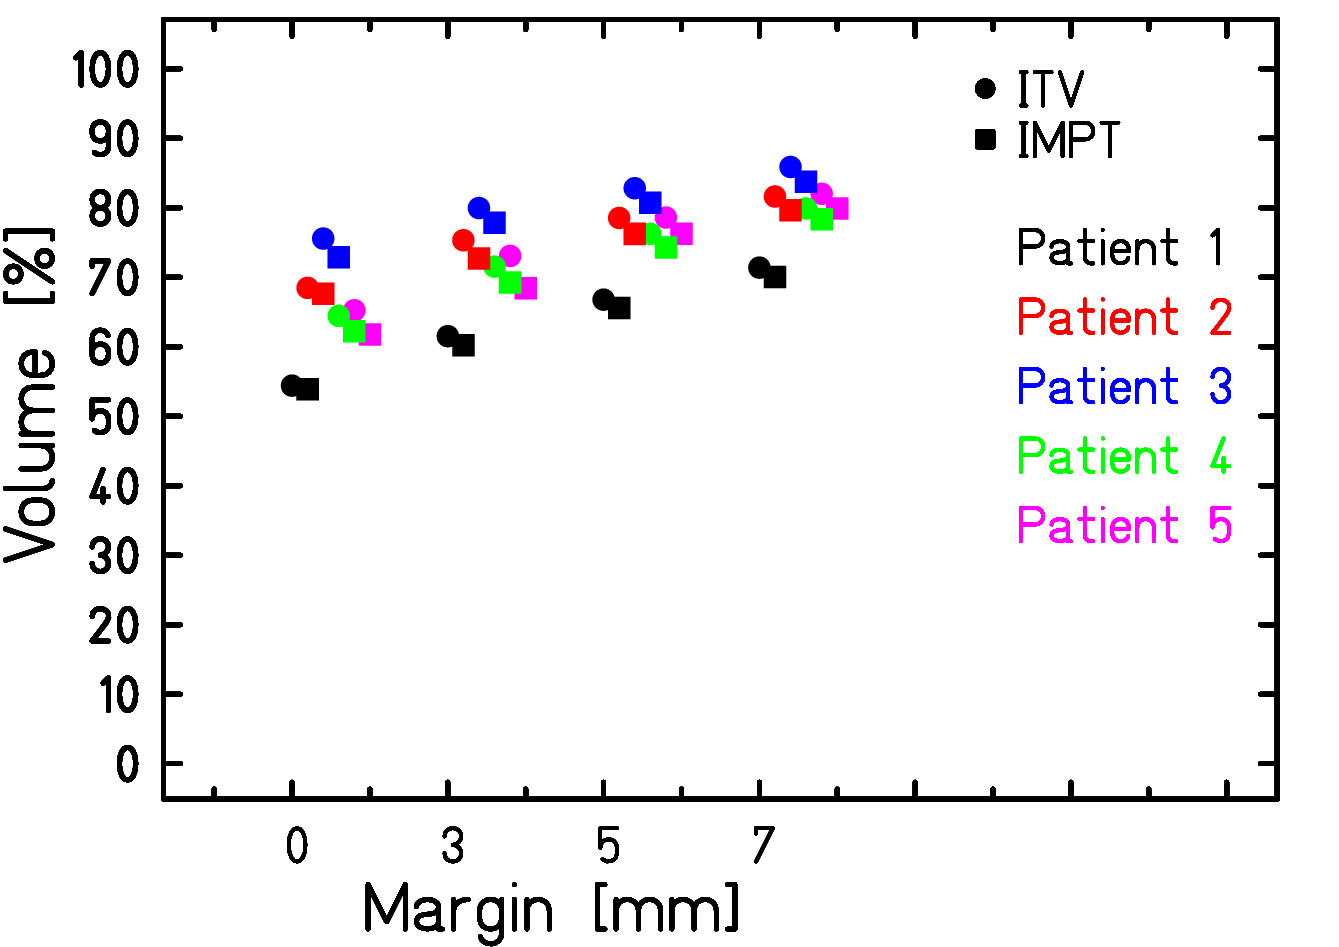
\includegraphics[scale=0.18]{Mayo_Human_LA_MaxVolume.png}
%  }
%  \subfigure[Maximum volume: RA]{
%  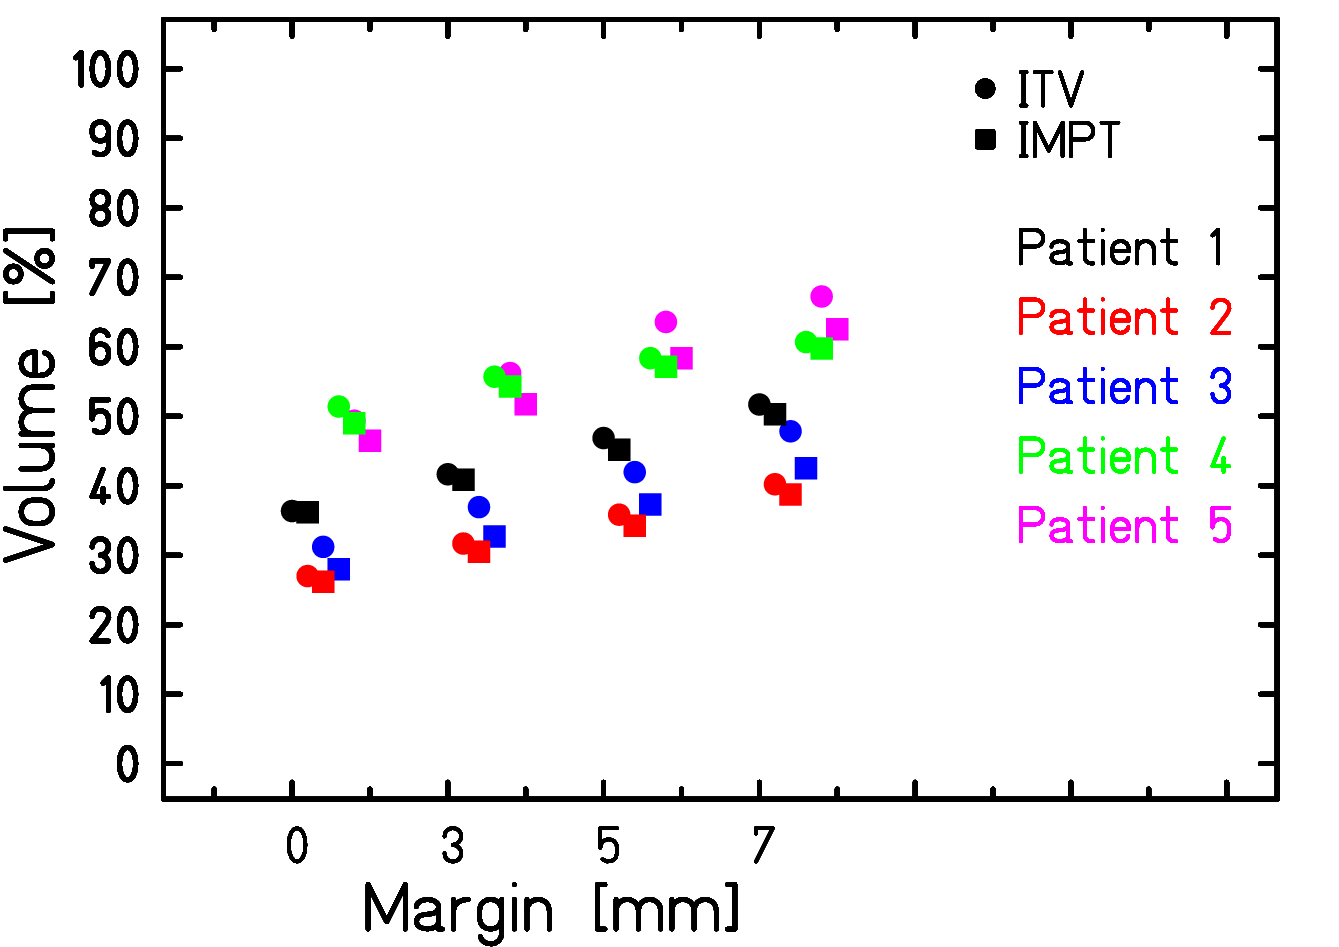
\includegraphics[scale=0.18]{Mayo_Human_RA_MaxVolume.png}
%  }
% \caption{Mean dose, maximal point dose and maximal irradiated volume of left atrium (LA) and right atrium (RA), respectively, when irradiating the LPV 
% and RPV in the five patient data sets with different margins (0 mm, 3 mm, 5 mm, 7mm) and two different delivery techniques (SFUD irradiation and IMPT).}
% \label{static_margin_dose_atria}
% \end{figure}


% % \begin{figure}[H]
% % \begin{center}
% % \subfigure[AV node: mean dose]{
% %  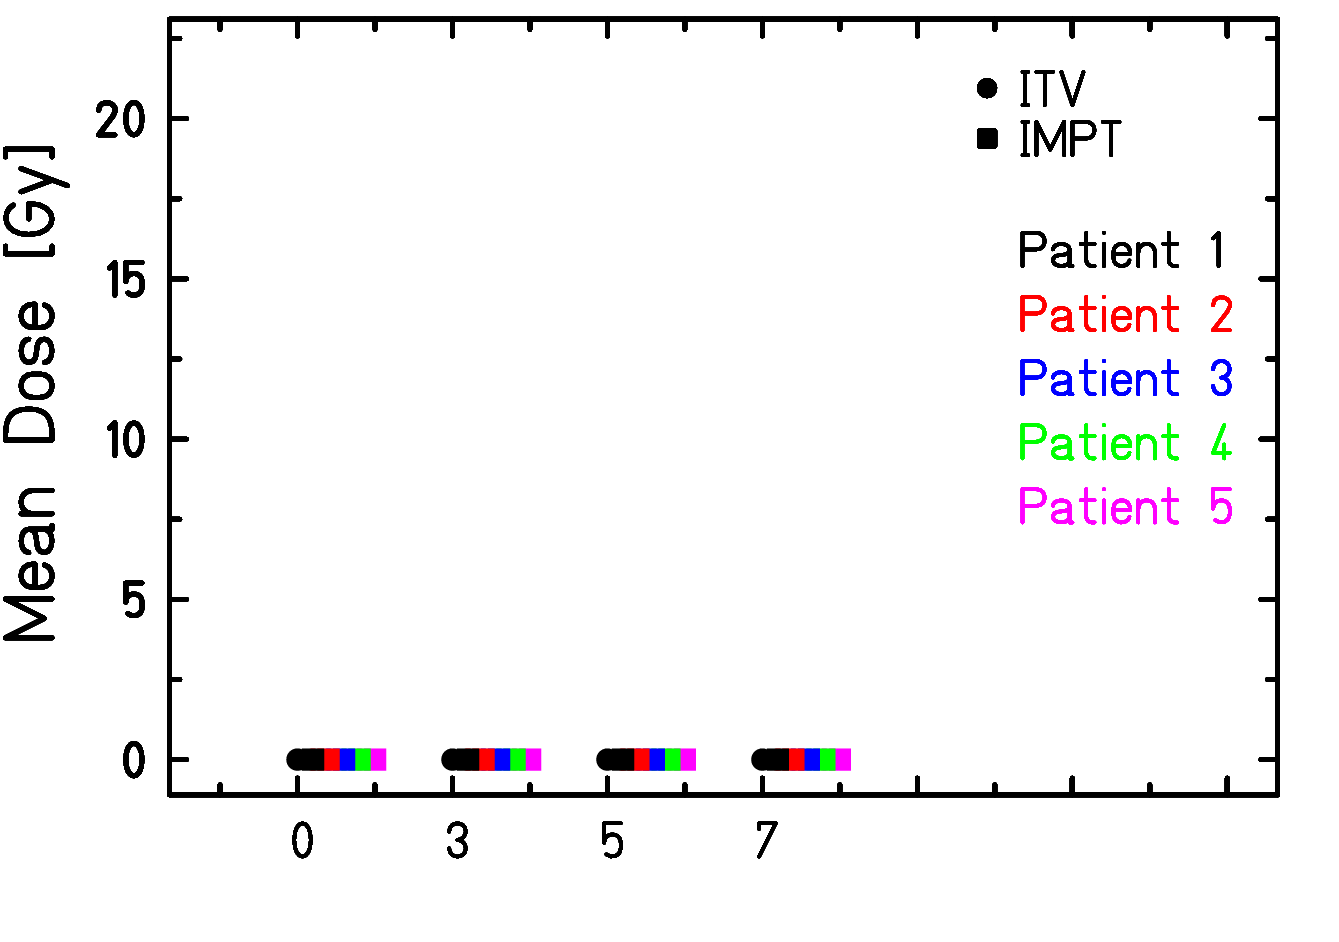
\includegraphics[scale=0.18]{Mayo_Human_AV_MeanDose.png}
% %  }
% %  
% %  \subfigure[AV node: maximum point dose]{
% %  \includegraphics[scale=0.18]{Mayo_Human_AV_MaxDose.png}
% %  }
% %  
% %  \subfigure[AV node: maximum volume]{
% %  \includegraphics[scale=0.18]{Mayo_Human_AV_MaxVolume.png}
% %  }
% % \caption{Mean and maximum dose to the AV node and maximal irradiatied AV node volume when irradiating the LPV and RPV in the five patient data sets with 
% % different margins (0 mm, 3 mm, 5 mm, 7mm) and two different delivery techniques (SFUD irradiation and IMPT).}
% % \label{static_margin_dose_heart}
% % \end{center}
% % \end{figure}


\newpage

\subsection{Motion assessment of heartbeat}
% \vspace*{-0.7cm}
Using the resulting deformation maps from deformable image registration the motion of the ablation sites of LPV and RPV was assessed. Motion 
volume histograms (MVHs) \cite{Ric13} displaying the relative displacement of every voxel of the investigated volume to the reference phase in 
all three motion directions were generated. The mean and standard deviation of these displacement values in each motion phase of LPV and RPV 
are plotted for all patients and motion directions in figure \ref{fig:motion_hb_lpv} and \ref{fig:motion_hb_rpv}, respectively.\newline
\newline
The mean and standard deviation of each patient over all motion phases are stated in table \ref{tab:motion_pv}. 
From the five studied patients patient 4 is displaying the highest absolute displacement, both in LPV and RPV. 
Furthermore it can be seen that none of the motion directions can be determined as the largest contribution to the absolute displacement, 
neither in LPV or RPV motion. 
% While the largest contribution to the LPV displacement in patient 1 is e.g. in the AP direction, patient 4 on 
% the other hand shows the largest displacement in SI direction. 
In table \ref{tab:maxabs_pv} the maximal absolute displacement for each patient is presented together with the corresponding motion 
phase. While motion phase six is the motion phase with the biggest displacement in 30\% of all cases, no evident maximal motion phase can be 
assessed. On average, the absolute amplitude over all motion phases and patients is found to (2.71 $\pm$ 1.57)mm for LPV and 
(2.62 $\pm$ 1.41)mm for RPV. In SI direction, the mean amplitude is (-0.60 $\pm$ 1.36)mm for LPV and (-0.17 $\pm$ 1.57)mm for RPV. In AP 
direction it is (0.77 $\pm$ 0.96)mm for LPV and (1.00 $\pm$ 1.58)mm for RPV, while in LR direction it is found to (0.36 $\pm$ 0.92)mm for LPV 
and (-1.00 $\pm$ 1.48)mm for RPV. Hence, averaged over all patients it can be stated that the PVs are moving mostly in AP direction. 
Nevertheless the contribution of the other motion directions are in the same order of magnitude.\newline 
\newline
The motion phases of the heartbeat gated CT scan are based on the ECG trace and result in a division of a single heartbeat. The 
motion phases can hence be directly assigned to the contraction (systole) and dilatation (diastole) of both atria and ventricles.  
Contraction of the atria (atrial systole) is occurring in between motion phase four and nineteen, in the same time as the ventricular relaxation 
(ventricular diastole). The ventricular systole and at the same time atria diastole are hence much shorter, occurring in the 
remaining motion phases twenty to three. The maximal displacement of the atria should thus be observed in motion phase eightteen, while the 
maximal amplitude of the ventricle should be observed in motion phase three. The motion of the PVs on the other hand result in a much more 
chaotic displacement. No motion phase can be assessed to a maximal displacement in all patient cases and no dominant motion direction is 
observed. The underlying heartbeat motion which causes the PVs to move should hence be much more complex. 
% \newline
% \newline

% %%%%%%% RESPIRATION %%%%%%
% \subsubsection{Respiration}
% 
% \begin{figure}[H]
% \begin{center}
%  \includegraphics[scale=0.2]{Mayo_Pat02_RESP.png}
% \caption{Motion amplitude of PVs under influence of respiration for Patient 1 in all motion directions (ABS: absolute, SI: superior-inferior, 
% AP: anterior-posterior, LR: left-right). LPV motion is displayed in black, RPV motion in red.}
% \end{center}
% \label{motion_resp}
% \end{figure}
% 
% \begin{figure}[H]
% \begin{center}
%  \includegraphics[scale=0.25]{Contour_z_abs_RESP_Pat02_gedreht.png}
% \caption{Contour plot of Respiration in Patient 1. }
% \end{center}
% \label{contour_pat02}
% \end{figure}


% \newpage
% %%%%%%% HEART BEAT %%%%%%
% \subsubsection{Heartbeat}

\newpage

\begin{figure}[H]
\begin{center}
 \includegraphics[scale=0.25]{MAYO_allPatients_HB_LPV.png}
\caption{Motion amplitude of LPV under influence of heartbeat for all patients. (Patient 1: black, Patient 2: red, Patient 3: green, 
Patient 4: blue, Patient 5: turquois) }
\label{fig:motion_hb_lpv}
\end{center}
\end{figure}

\vspace*{-1.3cm}

\begin{figure}[H]
\begin{center}
 \includegraphics[scale=0.25]{MAYO_allPatients_HB_RPV.png}
\caption{Motion amplitude of RPV under influence of heartbeat for all patients. (Patient 1: black, Patient 2: red, Patient 3: green, 
Patient 4: blue, Patient 5: turquois) }
\label{fig:motion_hb_rpv}
\end{center}
\end{figure}

\newpage

\vspace*{1cm}

\begin{table}[H]
  \centering
  \caption{Mean displacement of PVs over all motion phases (MP) in all patients and motion directions.}
  \begin{tabular}{|c|c|c|c|c|}
    \hline\hline
    Patient & LPV: ABS [mm] & LPV: SI [mm] & LPV: AP [mm] & LPV: LR [mm] \\
    \hline
    1 & 2.71 $\pm$ 1.18 & -1.17 $\pm$ 0.91 & 1.35 $\pm$ 1.08 & -0.89 $\pm$ 0.75 \\
    2 & 2.31 $\pm$ 1.14 & 1.16 $\pm$ 1.10 & 0.63 $\pm$ 0.53 & -1.38 $\pm$ 0.90 \\
    3 & 2.48 $\pm$ 1.75 & -0.36 $\pm$ 1.07 & 0.54 $\pm$ 0.78 & -1.18 $\pm$ 1.95 \\
    4 & 4.27 $\pm$ 2.54 & -3.07 $\pm$ 2.49 & 0.34 $\pm$ 1.43 & -0.78 $\pm$ 2.47 \\
    5 & 2.15 $\pm$ 1.23 & -0.75 $\pm$ 1.44 & 0.67 $\pm$ 1.10 & -0.18 $\pm$ 0.94 \\
    \hline\hline
    Patient & RPV: ABS [mm] & RPV: SI [mm] & RPV: AP [mm] & RPV: LR [mm] \\
   \hline
    1 & 2.12 $\pm$ 0.71 & -0.88 $\pm$ 0.65 & 1.11 $\pm$ 0.87 & 0.60 $\pm$ 0.60 \\
    2 & 2.25 $\pm$ 1.28 & 0.70 $\pm$ 1.15 & 0.96 $\pm$ 1.07 & -1.19 $\pm$ 1.01 \\
    3 & 2.22 $\pm$ 1.19 & 0.23 $\pm$ 1.25 & 0.50 $\pm$ 1.77 & 0.39 $\pm$ 0.70 \\
    4 & 4.62 $\pm$ 2.33 & -1.68 $\pm$ 3.12 & 1.67 $\pm$ 2.82 & 1.84 $\pm$ 0.94 \\
    5 & 2.77 $\pm$ 1.72 & 0.22 $\pm$ 1.77 & 1.03 $\pm$ 1.25 & 1.40 $\pm$ 1.40 \\
    \hline\hline
  \end{tabular}
  \label{tab:motion_pv}
\end{table}

\begin{table}[H]
  \centering
  \caption{Biggest absolute displacement of PVs with corresponding motion phase (MP) in all patients.}
  \begin{tabular}{|c|c|c|}
    \hline\hline
    Patient & LPV: max. ABS [mm] & MP \\
    \hline
    1 & 4.50 $\pm$ 1.72 & 06 \\
    2 & 5.26 $\pm$ 1.92 & 06 \\
    3 & 3.39 $\pm$ 2.24 & 08 \\
    4 & 5.52 $\pm$ 3.06 & 11 \\
    5 & 2.92 $\pm$ 1.54 & 16 \\
    \hline\hline
   Patient & RPV: max. ABS [mm] & MP \\
   \hline
    1 & 3.99 $\pm$ 1.40 & 06 \\
    2 & 5.20 $\pm$ 1.80 & 04 \\
    3 & 2.93 $\pm$ 1.35 & 11 \\
    4 & 6.49 $\pm$ 3.00 & 10 \\
    5 & 3.95 $\pm$ 3.95 & 15 \\
    \hline\hline
  \end{tabular}
  \label{tab:maxabs_pv}
\end{table}

\newpage

The overall displacement field between the extreme states of the ventricular displacement (motion phase three) and atrial displacement 
(motion phase eightteen) for two exemplary patients with a small motion amplitude (patient 5) and a large motion amplitude (patient 4) are 
shown in figure \ref{contour_plot_hb}. In order to visualize the location of the displacement, an axial cut of the reference state CT is 
underlayed. The absolute values of the displacement vectors are shown as contour plots. 

\begin{figure}[H]
\subfigure[Patient 4: max motion ventricle]{
 \includegraphics[scale=0.18]{Contour_z_abs_HB_Pat08_03_newSkala_gedreht.png}
}
\subfigure[Patient 5: max motion ventricle]{
\includegraphics[scale=0.18]{Contour_z_abs_HB_Pat10_03_newSkala_gedreht.png}
}
\subfigure[Patient 4: max motion atria]{
 \includegraphics[scale=0.18]{Contour_z_abs_HB_Pat08_18_newSkala_gedreht.png}
}
\subfigure[Patient 5: max motion atria]{
\includegraphics[scale=0.18]{Contour_z_abs_HB_Pat10_18_newSkala_gedreht.png}
}
\caption{Axial slices of the reference state of the CT overlayed with the absolute values of the displacement field (obtained from 
deformable image registration) in the corresponding slice for heartbeat motion. In the top row the displacement from the motion phase with the 
maximal ventricle motion to the reference phase is shown, in the lower row the displacement from the motion phase with the maximal 
atrial motion, for Patient 4 and Patient 5, respectively.}
\label{contour_plot_hb}
\end{figure}


\newpage
\subsection{Motion mitigation techniques for heartbeat}

The absolute motion amplitudes of up to 5mm due to heartbeat are expected to yield dose inhomogeneities when not compensated for. The 
resulting Interplay effect and dose deposition was studied for every patient for different motion patterns and different margins to the target 
volumes. The dose analysis values V95, V107 and D5-D95 were assessed and plotted. For comparison also the corresponding 
values for the 3D case (static) are shown. Due to the small motion amplitude, rescanning was studied as motion mitigation technique.  
The results of the stated dose values in case of rescanning with different rescan numbers will also be presented. 


\subsubsection{Dose deposition}
A representative dose deposition for all studied techniques (static, interplay and rescanning with ten rescans) is shown exemplary for patient 
4 (as this is the patient with the largest PV motion amplitude both in LPV and RPV) in figure \ref{dose_pat08}. Rescanning and interplay are 
shown for a sinus motion with a period of 0.7s and a starting phase of 0$^{\circ}$. The target volumes LPV and RPV were irradiated 
simultaneously and a margin of 3mm was added. It can already been seen from this dose cut figures that rescanning with only ten rescans drastically 
improves the outcome compared to interplay and yields a result which is comparable to the static case.\newline
\newline
For patient 4, the different motion patterns DVHs of ten rescans compared to the interplay results as well as a static irradiation are 
displayed in figure \ref{dvhs_pat08} for 3mm safety margin. 
In order to assess the dose information of all patients the DVHs were analyzed and compared for dose steepness, dose coverage as well as over dosage. The average results 
over all patients with the resulting standard deviation can be seen in figure \ref{static_interplay_rescanning_ALL}. A more detailed analysis 
can be found in appendix XXX, where the values are plotted for each patient (figures \ref{static_interplay_rescanning_Pat01} - 
\ref{static_interplay_rescanning_Pat05}) and all corresponding numerical values are shown (tables \ref{tab:Pat02_LPV} - \ref{tab:Pat10_RPV}).\newline
\newline
For interplay it can be seen that the results are dependent on the used motion period and starting phase. This can be seen in the mean values 
of dose parameter value results for different, underlying motion patterns. E.g. for the RPV, the mean value of the dose coverage parameter 
over all patients is V95=(88.8 $\pm$ 12.8)\% for a sinus motion with 1s period and a starting phase of 90$^{\circ}$ and 
(98.01 $\pm$ 1.36)\% for a sinus motion with 0.7s period and a starting phase of 90$^{\circ}$, while for a sinus motion with 0.7s period 
and a starting phase of 0$^{\circ}$ the dose coverage is found to (92.1 $\pm$ 12.7)\%. The resulting high standard deviation over all patient 
cases shows that the result is also dependent on the studied patient case. Furthermore the result is also dependent on the studied safety 
margin, so that e.g. the dose coverage for a sinus motion with 1s period and a starting phase of 90$^{\circ}$ results to (95.9 $\pm$ 2.4)\%
with 3mm safety margin. All these dependencies are also valid for the other studied dose analysis parameters, dose homogeneity and over dosage.\newline
\newline
The underlying deformation map with its motion amplitude does not enable a prediction of the magnitude of the 
interplay effect. This was studied in more detail for the dose coverage parameter V95. Here, the correlation between the maximal absolute 
motion amplitude of the left and right PV (see table \ref{tab:maxabs_pv}) and the resulting V95 value for 3 mm Margin were assessed for all 
studied motion patterns (sinus motion with period of 1s or 0.7s and starting phase of 0$^{\circ}$ and 90$^{\circ}$) and patients. The results 
can be seen in figure \ref{corr_maxabs_V95_interplay}.  A moderate correlation between the dose coverage and maximal amplitude resulted only 
in the case of RPV where a motion period of 0.7s with a starting phase of 90$^{\circ}$ was chosen (r=0.49; p<0.05). Nevertheless these results 
could not be verified in the other motion cases and in the irradiation of the LPV and hence no dependence between target volume displacement 
and dose coverage in case of interplay was found.\newline
\newline
As can be seen in figure \ref{static_interplay_rescanning_ALL} (as well as in more detail for all patients in appendix XXX) 
rescanning yields improved results compared to interplay in all studied cases. This is valid for dose steepness, dose 
coverage as well as over dosage. Especially dose coverage and over dosage are comparable to the static results for all patient and motion patterns.  
Exemplary, the dose coverage of patient 4 (with the largest absolute displacement) will be discussed. V95 for a static irradiation of the LPV 
of patient 4 with 3mm safety margin is found to 99.8\%. With a motion of 0.7s period length and a starting phase of 0$^{\circ}$ the value  
decreases to 90.0\%. With rescanning, V95 can be improved to 99.75\% with only five rescans. Also for RPV the static dose coverage 
with 3mm margin is found to 100\% for this patient. With the stated motion and safety margin the dose coverage decreases to 97.0\%  
in the case of interplay. With five rescans the value improves again to 100.0\%. The improvement of dose coverage and over dosage 
compared to interplay is valid for all studied rescan numbers, starting from the smallest studied rescan number of five, as shown here. 
Nevertheless, in some studied cases five rescans is not enought to yield results comparable to the static irradiation. For example for the LPV 
irradiation with five rescans in patient 1 with a motion period of 1s and 90$^{\circ}$ starting phase (3mm safety margin) V95 results in a 
smaller dose coverage (93.2\%) than the static case (100\%). Even though this result is improved compared to interplay (86.9\%), a much 
better result can be gained with higher rescan numbers, starting with ten rescans (99.2\%). Also the results for dose homogeneity improves 
with higher rescan numbers. For a motion pattern of 0.7s period and 0$^{\circ}$ starting phase (3mm safety margin) in patient 4, the dose 
homogeneity in case of interplay is found to 9.9\%. With five rescans a dose homogeneity of 5.5\% is yielded, which further decreases to 
4.6\% with ten rescans, 4.4\% with fifteen rescans and 3.9\% with twenty rescans (compared to 3.9\% in the static irradiation). 
It can thus be conluded that rescan numbers higher than five yield better slightly results, while ten rescans show results comparable to the 
static irradiation in all studied patient cases, for all studied safety margins and for all underlying motion patterns. As can be furthermore 
seen in figure \ref{static_interplay_rescanning_ALL}, the standard deviation of the dose analysis parameters over all patients is 
rather small for ten and higher rescan numbers, proving the robustness of rescanning as a motion mitigation technique for a displacement of 
the PVs due to heartbeat.

\vspace*{-0.3cm}

 \begin{figure}[H]
 \begin{center}
\subfigure[LPV]{
 \includegraphics[scale=0.28]{Pat08_LPV_allDVHs_newColor_withLegend.png}
 }
\subfigure[RPV]{
 \includegraphics[scale=0.28]{Pat08_RPV_allDVHs_newColor_withLegend.png}
 }
\caption{Dose volume histograms for CTV of patient 4 for 3mm safety margin irradiation (LPV (a) as well as RPV (b)) in case of static 
irradiation (black), interplay (dashed) and rescanning with ten rescans (solid). The motion patterns are shown in colors (sin1s0: sinus with motion period of 1s 
and starting phase 0$^{\circ}$, sin1s90: sinus with motion period of 1s and starting phase 90$^{\circ}$, sin07s0: sinus with motion period of 0.7s 
and starting phase 0$^{\circ}$, sin07s90: sinus with motion period of 0.7s and starting phase 90$^{\circ}$.}
\label{dvhs_pat08}
 \end{center}
\end{figure}

\newpage
 \begin{figure}[H]
 \begin{center}
\subfigure[static]{
 \includegraphics[scale=0.36, angle=180]{Pat08_static_withLegend.png}
 }
\subfigure[interplay]{
 \includegraphics[scale=0.36, angle=180]{Pat08_interplay_withLegend.png}
 }
 \subfigure[rescanning (10x)]{
 \includegraphics[scale=0.36, angle=180]{Pat08_10rescans_withLegend.png}
 }
\caption{Dose distribution of patient 4 for static (a) as well as interplay (b) and ten rescans (c) at motion period of 0.7s and a motion 
starting phase of 0$^{\circ}$. The target volume has an added margin of 3mm. The improved outcome of rescanning compared to interplay 
can already be seen in these dose cuts.}
\label{dose_pat08}
 \end{center}
\end{figure}


\newpage
% \vspace*{-0.3cm}
\begin{figure}[H]
\subfigure[D5-D95: LPV]{
 \includegraphics[scale=0.18]{MAYO_CTV_LPV_D5D95_ALL.png}
 }
 \subfigure[D5-D95: RPV]{
 \includegraphics[scale=0.18]{MAYO_CTV_RPV_D5D95_ALL.png}
 }
 \subfigure[V95: LPV]{
 \includegraphics[scale=0.18]{MAYO_CTV_LPV_V95_ALL.png}
 }
\subfigure[V95: RPV]{
 \includegraphics[scale=0.18]{MAYO_CTV_RPV_V95_ALL.png}
 }
  \subfigure[V107: LPV]{
 \includegraphics[scale=0.18]{MAYO_CTV_LPV_V107_ALL.png}
 }
\subfigure[V107: RPV]{
 \includegraphics[scale=0.18]{MAYO_CTV_RPV_V107_ALL.png}
 }
\caption{Mean and standard deviation of dose analysis parameters D5-D95 (first row), V95 (middle row) and V107 (last row) over all patients. 
The LPV (left column) and RPV (right column) were studied seperately. Static (black) as well as interplay (red) and different rescanning 
numbers (5 times: turquois, 10 times: blue, 15 times: light green, 20 times: dark green) were compared for different motion patterns and 
safety margins. For a better visualization the rescanning data points for each motion pattern are shifted.}
\label{static_interplay_rescanning_ALL}
\end{figure}

\newpage
\begin{figure}[H]
\centering
\subfigure[LPV: sinus, period 1s, phase 0$^{\circ}$]{
 \includegraphics[scale=0.58]{Corr_V95_LPV_sin1s0.png}
 }
\subfigure[RPV: sinus, period 1s, phase 0$^{\circ}$]{
 \includegraphics[scale=0.58]{Corr_V95_RPV_sin1s0.png}
 }
\subfigure[LPV: sinus, period 1s, phase 90$^{\circ}$]{
 \includegraphics[scale=0.58]{Corr_V95_LPV_sin1s90.png}
 }
\subfigure[RPV: sinus, period 1s, phase 90$^{\circ}$]{
 \includegraphics[scale=0.58]{Corr_V95_RPV_sin1s90.png}
 }
\subfigure[LPV: sinus, period 0.7s, phase 0$^{\circ}$]{
 \includegraphics[scale=0.58]{Corr_V95_LPV_sin07s0.png}
 }
\subfigure[RPV: sinus, period 0.7s, phase 0$^{\circ}$]{
 \includegraphics[scale=0.58]{Corr_V95_RPV_sin07s0.png}
 }
\subfigure[LPV: sinus, period 0.7s, phase 90$^{\circ}$]{
 \includegraphics[scale=0.58]{Corr_V95_LPV_sin07s90.png}
 }
\subfigure[RPV: sinus, period 0.7s, phase 90$^{\circ}$]{
 \includegraphics[scale=0.58]{Corr_V95_RPV_sin07s90.png}
 }
\caption{Interplay dose homogeneity of LPV (left column) and RPV (right column) in all patients in relation to the maximal absolute 
displacement of the PVs and for different underlying motion patterns (first row: sinus with 1s period and starting phase of 0$^{\circ}$, 
second row: 1s period and starting phase of 90$^{\circ}$, third row: 0.7s period and starting phase of 0$^{\circ}$, last row: 0.7s period 
and starting phase of 90$^{\circ}$).}
\label{corr_maxabs_V95_interplay}
\end{figure}

\newpage

\subsubsection{Irradiation time}
In figure \ref{irrTime_all} the mean irradiation time over all patients for different rescanning irradiations of LPV and RPV are shown for 
different safety margins and motion patterns. The duration for each beam entry channel (gantry angle of -45$^{\circ}$, 135$^{\circ}$ and 0$^{\circ}$) 
is plotted individually. It can be seen that the needed irradiation time increases with the used safety margin as the to irradiated volume 
increases. The irradiation time is independent of the motion pattern but varies depending on the used beam entry channel. 
Concerning the used rescan number it can be seen that no treatment prolongation is expected for higher rescan numbers. 
This can be understood as with higher rescans the intensity of each raster point in one iteration is reduced by a factor which is equal to 
the rescanning number. Hence the time the beam has to spend in one raster position, depositing the predetermined intensity, is reduced  
resulting in an overall treatment time which is constant for all rescan cases. The stated results were achieved with a low intensity irradiation 
(minimal particle number of 5.000). For an irradiation with 3mm margin around LPV and RPV the overall treatment time results to (13.71 $\pm$ 
0.94)min (see table \ref{tab:rescan_time}) with rescanning as motion mitigation technique for heartbeat motion.

 \begin{figure}[H]
 \begin{center}
 \includegraphics[scale=0.2]{All_irrTime.png}
\caption{Mean and standard deviation of the irradiation time over all patients for different rescan numbers, underlying motion patterns and beam entry 
channels.}
\label{irrTime_all}
 \end{center}
\end{figure}

\begin{table}[H]
  \centering
%   \footnotesize
  \caption{Mean irradiation time for LPV and RPV with a safety margin of 3mm over all patients.}
  \begin{tabular}{|c|c|c|}
    \hline\hline
    Gantry angle [$^{\circ}$] & time [min] & total [min] \\
    \hline
    -45 & 4.73 $\pm$ 0.93 & \\
    135 &  4.42 $\pm$ 0.94 & 13.71 $\pm$ 0.94\\
    0 & 4.56  $\pm$ 0.96 & \\
    \hline\hline
    \end{tabular}
  \label{tab:rescan_time}
\end{table}

% % \begin{table}[H]
% %   \centering
% %   \footnotesize
% %   \caption{Mean irradiation time for LPV and RPV with a safety margin of 3mm over all patients.}
% %   \begin{tabular}{|c|c|c|c|}
% %     \hline\hline
% %     Rescan number & Gantry angle [$^{\circ}$] & time [min] & total [min] \\
% %     \hline
% %      & -45 & 4.73 $\pm$ 0.93 & \\
% %     5 & 135 &  4.42 $\pm$ 0.94 & 13.71 $\pm$ 1.63\\
% %      & 0 & 4.56  $\pm$ 0.96 & \\
% %     \hline
% %      & -45 & 4.73 $\pm$ 0.93 &  \\
% %     10 & 135 & 4.42 $\pm$ 0.94 & 13.71 $\pm$ 1.63 \\
% %      & 0 & 4.56 $\pm$ 0.96 &  \\
% %     \hline
% %      & -45 & 4.73 $\pm$ 0.93 &  \\
% %     15 & 135 & 4.42 $\pm$ 0.94 & 13.71 $\pm$ 1.63 \\
% %      & 0 & 4.56 $\pm$ 0.96 &  \\
% %     \hline
% %      & -45 & 4.73 $\pm$ 0.93 &  \\
% %     20 & 135 & 4.42 $\pm$ 0.94 & 13.71 $\pm$ 1.63 \\
% %      & 0 & 4.56 $\pm$ 0.96 &  \\
% %     \hline
% %     \hline\hline
% %     \end{tabular}
% %   \label{tab:rescan_time}
% % \end{table}

\newpage

\section{Discussion}

In this chapter the influence of heartbeat motion on the PVs was studied and treatment planning studies with rescanning as motion 
mitigation technique were carried out. A detailed analysis of the dose depositions to the OAR was performed, with special 
emphasis on the irradiation of cardiac substructures. Beforehand, a study of the best suited field number and beam directions was  
conducted as well as an analysis of possible safety margin limitations. 


\subsection{Dose to critical structures}
\label{Discussion:doseOAR}

Concerning the dose deposition in OAR (esophagus, trachea, aorta and heart) dose-volume limits from SBRT were used. In SBRT 
treatment a high dose is also applied in a single fraction and hence comparable to the here stated dose delivery of 25Gy physical 
dose in one treatment session. 
An extensive collection of dose-volume-limits for SBRT are presented in the study protocols of the Radiation Therapy Oncology Group (RTOG). 
The there stated dose-volume lmits for trachea (10.5Gy in 4cm$^{3}$) and aorta (31Gy in 10cm$^{3}$) were not exceeded for any of the studied field 
numbers and beam channel combinations. The same is valid while keeping the chosen three fields (couch angle of 90$^{\circ}$ 
and gantry angles of -45$^{\circ}$, 135$^{\circ}$ and 0$^{\circ}$) constant and changing the studied safety margins (0mm, 3mm, 5mm and 7mm). 
For the esophagus on the other hand, the dose-volume limits were much more critical. Most of the studied beam directions yielded a dose 
which exceeded the stated dose-volume limit (11.9Gy for 5cm$^{3}$). Hence an IMPT delivery, including the esophagus in the 
optimization process, was necessary. With this delivery technique and the above stated beam direction, the dose to the esophagus could be 
drastically reduced,. Nevertheless only an irradiation of the PVs with 3mm safety margin resulted in a dose deposition into the esophagus 
which met the dose volume limit (median of 9.3Gy, 75th percentile: 12.1Gy). This result could be drastically improved with different IMPT 
parameters, enabling a safe irradiation when patient specific IMPT parameters were used. 
Thus also safety margins higher then 3mm should result in a uncritical dose deposition. 
For the heart all beam channels, safety margins and delivery types (SFUD or IMPT) exceeded the stated dose-volume limit (16Gy for 15cm$^{3}$). 
This is due to the fact that the heart is not only an OAR in the here presented, non-invasive treatment modality for PV isolation, 
but part of the cardiac structures are also the target itself. Hence a closer look on the affected cardiac substructures and 
the relevance of these dose depositions on cardiac toxicity and late effects were given.\newline
\newline
QUANTEC (quantitative analysis of normal tissue effects in the clinic) \cite{QUANTEC10} offers an comprehensive literature review 
on the available data of the last 20 years and is meant as an update of the extensively used dose-limits proposed by Emami et al. 
\cite{Ema91}. In the QUANTEC publication by Gagliardi et al. \cite{Gag10} radiation dose-volume effects in the heart are presented. 
It is stated that radiation-induced cardiac diseases are distinguished between acute injuries like pericarditis\footnote{inflammation 
of the sac containing the heart}, which can turn into a chronic disease, and late injuries which manifest months or even 
years after radiation exposure. Typical late injuries are congestive heart failure\footnote{heart is unable to maintain sufficient 
blood flow}, ischemia\footnote{deficient blood supply}, coronary artery disease and myocardial infarction\footnote{heart attack}. 
It was summarized that it remains uncertain which region of the heart is most important for radiation induced tissue toxicities. 
But it is stated that the risk of cardiac events is probably related to both dose and irradiated volume. 
Pericarditis seems to be related to left ventricle (LV) irradiation, and it was found that LV shielding was able to drastically 
reduce the incidence rate \cite{Carm76}. It was stated that a mean cardiac dose of 27.1Gy and maximum dose of 47Gy seem to act as 
predictors for pericarditis \cite{Mar98}. 
% and a fraction size of smaller than 3.5 Gy per fraction did not result in pericarditis. 
Wei et al. \cite{Wei08} stated another discriminator for pericarditis which was found to be V30 < 46\%, which translates in a mean 
pericardial dose of less than 26Gy. For coronary and ischemic events relevant substructcm$^{3}$ures are assumed to be coronary arteries on 
the left ventricle (LCA) \cite{Nie07} \cite{Tay07} \cite{Tay08}. Furthermore it is stated that excess deaths from heart disease are observed 
in patients receiving more than 42Gy \cite{Han93} and that aortic and mitral stenosis incidences increased above a threshold dose of 
30Gy \cite{Tay07}. For long term cardiac mortality an increased rate was only observed at whole heart doses above 30Gy \cite{Han93}.\newline
\newline
Hooning et al. \cite{Hoo07} studied the cardiovascular disease incidence in more than 4000 breast cancer survivors 
after a follow-up period of more than 10 years as patients were treated from 1970 through 1986. It was the first study to examine the 
effects of cardiovascular risk factors in combination to radiotherapy. They found that the risk of congestive heart failure was 
significantly increased when the patients had received chemotherapy (95\% confidence interval of 1.25 to 2.73) and that smoking drastically 
increased the risk of the patients to suffer a myocardial infarction (95\% confidence interval of 2.03 to 4.55). Concerning 
radiotherapy they stated that a higher mean dose to the whole heart resulted in an increased risk of congestive heart failure and 
that an irradiation of the left vs right chest wall (thus more heart volume and in particular including the LV and apex) led to an 
increased risk of myocardial infarction.\newline
\newline
A recent study by Darby et al. \cite{Dar13} investigated more than 2000 breast cancer patients treated in between 1958 and 2001 
for coronary events like myocardial infarction, coronary revascularization or death from ischemic heart disease. The found a mean 
heart dose of 4.9Gy (0.03Gy to 27.72Gy) and that the rates of major coronary events increased linearly with the mean heart dose. 
They stated an increase of incidences by 7.4\% per Gy (95\% confidence interval of 2.9 to 14.5) after five years post radiotherapy.
\newpage
For the here studied seventeen beam channel combinations, applying a physical dose of 25Gy, the mean dose over all five studied patients was 
found to have a median of 1.26Gy (75th percentile: 1.48Gy). The median over the maximal point dose was 26.6Gy (75th percentile: 27.1Gy), 
while in general less than 30\% of the heart was irradiated. With the chosen field number of three beam channels with directions of a 
couch angle of 90$^{\circ}$ and gantry angles of -45$^{\circ}$, 135$^{\circ}$ and 0$^{\circ}$, the mean dose was found to less than 2Gy in all 
studied patient cases. For different added safety margins to the PVs it was found that the median mean dose over all patients was 
1.0Gy (75th percentile: 1.1Gy) with no margin, 1.3Gy (75th percentile: 1.5Gy) for 3mm, 1.4Gy (75th percentile:1.6Gy) for 5mm and 
1.5Gy (75th percentile: 1.6Gy) for 7mm margin. Hence, all these results are in good agreement to the dose and volume limitations 
stated in the above studies and thus no pericarditis should be expected when irradiating the PVs with an IMPT 
delivery of carbon ions. 
As the LV, and with it especially the LCA, are assumed to be radiosensitive structures within the heart the dose 
depositions to these structures were analyzed in more detail. It was found that three beam channel directions were best suited to yield a lower 
mean dose deposition in the LCA. Due to robustness criteria of the treatment delivery the above stated beam channel combination was 
chosen. With this delivery direction it was found that the mean dose to the LCA was, dependent on the used safety margin, 0.2Gy(75th 
percentile: 0.5Gy) with no margin, 0.5Gy (75th percentile: 0.5Gy) for 3mm margin, 0.7Gy (75th percentile: 1.1Gy) for 5mm and 
1.5Gy (75th percentile: 1.6Gy) for 7mm. The maximum point dose to the LCA with these beam channels nevertheless led to 
an increased dose in the left chamber compared to the right site. This is due to the proximity of the upper LCA branches 
to the LPV target site. 

\subsection{Beam channel directions and safety margins}
In general, it can be stated that field number and beam direction always result in a trade-off between dose to the OAR, irradiation time and 
robustness. While less fields and hence beam directions shorten the treatment time, it does lead to a less robust treatment. In case OAR are 
displaced during the treatment (intrafractional motion, see Introduction) or move in between CT image acquisition and irradiation 
(interfractional motion) beam channels with a large angle in between them are more robust, as not all fields are affected by this displacement 
and hence only a small dosis would be shifted. Furthermore, opposite fields (like -45$^{\circ}$ and 135$^{\circ}$ (see figure 
\ref{gantrydirection}) are more robust against potential range uncertainties and should hence be favored. Due to this reason, combined with 
the smaller LCA dose deposition in case of three field numbers, a couch angle of 90$^{\circ}$ and gantry angles of -45$^{\circ}$, 
135$^{\circ}$ and 0$^{\circ}$ was selected for the safety margin limitation studies as well as the motion mitigation treatment plans. 
Concerning safety margins, which need to be applied in order to account for possible deviations in between treatment planning and dose 
delivery, it can be stated that only a small margin tolerance was observed. This is due to the difficult position of the PVs close to 
radiosensitive structures like the esophagus and especially the heart. With IMPT treatment a delivery with 3mm safety margin was found to 
fulfill all the needed requirements. A more realistic safety margin of 5mm could be achieved with more restricted parameters in the IMPT 
optimization. 


% % % % %%% HEART: stimmt nicht
% % % % max point dose RTOG 22 Gy! alles drunter von den kritischen strukturen!


\subsection{Movement of PVs in cardiac cycle}

Lickfett et al. \cite{Lic05} analyzed the volume changes and displacement of the PVs in 25 healthy volunteers with MRI images. They 
studied the posterior edge of the PV orifice and observed that the size and location changed considerably during the cardiac cycle. 
Displacements of up to 7.2 mm were found and it could be concluded that the motion amplitudes were bigger in the coronal (left-right) 
than in the sagittal (anterior-posterior) direction. In more detail this largest coronal movement was found in the left superior PV, 
while the largest sagittal motion was observed in the right superior PV with 3.9 mm. The smallest saggital displacement was 2.5 mm in the 
left anterior PV. They suspected that the reason for movement is not resulting from a single influence, but is rather a mix of PV 
contraction, atrial contraction and ventricular force. The movement of PV due to heartbeat is also relevant for catheter ablation. Based 
on the stated finding Lickfett et al. recommended to keep a 5 mm distance from the PV orifice during PV encircling ablation in order to 
reduce the risk for PV stenosis. 
Patel et al. \cite{Pat08} on the other hand, who studied the MRI images of 30 patients in sinus rhythm with paroxysmal atrial fibrillation, 
stated that the displacement of the pulmonary veins was small. The left lower PV was found to move (2.7 $\pm$ 1.2) mm, the left upper PV 
(2.1 $\pm$ 1.1) mm, the right lower PV (1.9 $\pm$ 1.1) mm and the right upper PV (2.3 $\pm$ 1.0) mm.\newline 
% \newline
% The motion phases of the heartbeat gated CT scan are based on the ECG trace and result in a division of a single heartbeat. The 
% motion phases can hence be directly assigned to the contraction (systole) and dilatation (diastole) of both atria and ventricles.  
% Contraction of the atria (atrial systole) is occurring in between motion phase four and nineteen, in the same time as the ventricular relaxation 
% (ventricular diastole). The ventricular systole and at the same time atria diastole are hence much shorter, occurring in the 
% remaining motion phases twenty to three. The maximal displacement of the atria should thus be observed in motion phase eightteen, while the 
% maximal amplitude of the ventricle should be observed in motion phase three. The motion of the PVs on the other hand result in a . 
% The underlying heartbeat motion which causes the PVs to move should hence be much more complex and is probably influenced by a combination of 
% PV contraction, atrial contraction and ventricular force \cite{Lic05}. Thus the observed motion of the PVs is much more chaotic and no motion 
% phase can be assessed to a maximal displacement in all patient cases.
% % \newline
\newline
In the here studied patient cohort of five AF patients no differentiation between the upper and lower PVs was carried out. 
The motion was assessed for the whole potential ablation site of LPV and RPV, respectively. Similar to the study by Patel et al. only a small 
displacement was found, resulting to an average absolute displacement of less than 3mm (LPV: (2.71 $\pm$ 1.57)mm, RPV: (2.62 $\pm$ 1.41)mm). 
Even though a tendency to a higher motion in AP direction could be observed, the contributions of the other motion directions 
were in the same order of magnitude (up to 1mm). Hence no dominant motion direction could be determined. 
The motion phases of the heartbeat gated CT scan were based on the ECG trace and resulted in a division of a single heartbeat. Thus the motion 
phases could be directly assigned to the contraction (systole) and dilatation (diastole) of both atria and ventricles. 
Nevertheless no motion phase could be assessed to yield the maximum displacement. This reinforces the thesis by Lickfett et al. that the 
underlying heartbeat motion, which causes the PVs to move, is much more complex. 

\newpage

\subsection{Rescanning as motion mitigation technique}

Concerning dose deposition with rescanning compared to interplay it can be concluded that rescanning yields good result. 
Regarding dose coverage V95 values were higher than 99\% in 96.3\% of all studied cases with a safety margin of 3mm or higher. 
The minimum dose coverage over all studied cases with safety margin was found in patient 1, in the irradiation of the LPV with a margin 
of 3mm and an underlying motion of 1s period and 90$^{\circ}$ starting phase (V95=93.2\%). This result was obtained with five rescans. 
With higher rescans the dose coverage could be improved, so that only 1.5\% of the studied cases with ten or more rescans had a dose coverage 
smaller than 99\% (minimum: 97.1\%; 10 rescans in patient 1, 7mm safety margin and motion of 1s period and 90$^{\circ}$ starting phase). 
The dose coverage for rescans without safety margin was worse, resulting in 93.1\% cases under 99\%. 
V107 values higher than 0\% were obtained in 7.3\% of all cases with safety margin (maximum of V107=3.7\% in the LPV of patient 3 
with safety margin of 5mm, 5 rescans and motion of 1s period and 0$^{\circ}$ starting phase) compared to 
28.8\% of cases without safety margin (maximum: V107=8.0\% for the LPV of patient 2 with 5 rescans and motion of 1s period 
and 0$^{\circ}$ starting phase. This could be reduced to V107=2.9\% with 10 rescans). With safety margin, the dose homogeneity D5-D95 
did not exceed 8.9\%. Without safety margin D5-D95 did not exceed 10.2\%. Both of these values were achieved with 5 rescans and could be 
improved with 10 rescans (with safety margin to less than 7\% and without to less than 9\%). It can hence be concluded that additional 
safety margins enable a more robust and successful treatment delivery. However, if possible, these margins should be kept as small 
as technical feasible, as it increases the dose deposition in OARs. Regarding rescan numbers ten rescans yield improved results compared 
to five rescans. These results are not significantly improved with higher rescan numbers. 

\section{Conclusion}

The PVs were found to move due to heartbeat with an amplitude of up to 6mm. 
This displacement creates interplay effects when irradiated with carbon ions. Rescanning as motion mitigation technique was studied. 
It yields improved dose coverage and dose homogeneity compared to interplay in all studied patient cases, motion patterns and 
for all safety margins. It is thus an adequate motion mitigation technique for the irradiation of PVs under influence of heartbeat motion. 
A rescan number of ten is sufficient to obtain results comparable to the static irradiation. 
For the treatment delivery, IMPT dose optimization together with a rather small safety margin (of e.g. 3mm) results in dose depositions in the 
OARs (like esophagus as well as in the cardiac substructures) which are considered tolerable.  



%%%%%%%%%%%%%%%%%%%%%%%%%%%%%%%%%%%%%%%%%%%
%%%%%%%%%%%%%% APPENDIX %%%%%%%%%%%%%%%%%%%
%%%%%%%%%%%%%%%%%%%%%%%%%%%%%%%%%%%%%%%%%%%

\newpage

\section*{for APPENDIX}

% % % %%%%%%%%%%%%%%%%%%%%%%%%%%%%%%
% % % %%%%%% BEAM DIRECTION %%%%%%%%
% % % %%%%%%%%%%%%%%%%%%%%%%%%%%%%%%
% % % 
% % % \subsection*{Beam direction}
% % % 
% % % Complete data for all beam directions and patients. The volume in percent, corresponding to the respective volume of the dose volume 
% % % limits are stated (esophagus: 5 cc, trachea: 4 cc, heart: 15 cc and aorta: 10 cc) with the respective dose in percent. 
% % % If the DVHs were empty, and hence the OAR did not receive any dose, zero is stated in the tables. 
% % % 
% % % \begin{table}[H]
% % %   \centering
% % %   \caption{Patient 1, Esophagus: Percentage of volume and corresponding dose in percent}
% % %   \begin{tabular}{|c|c|c|c|c|}
% % %     \hline\hline
% % %     Field number & Couch angle & Gantry angle & Dose [\%] & Volume [\%]\\
% % %     \hline 
% % % 1FIELD & -90 & 0 & 3 & 11.8202 \\
% % % 1FIELD & -45 & 0 & 31 & 12.001 \\
% % % 1FIELD & -135 & 0 & 20 & 11.9235 \\
% % % 2FIELDS & 90 & -60/120 & 50 & 11.4714 \\
% % % 2FIELDS & 90 & -60/135 & 48 & 11.8719 \\
% % % 2FIELDS & 90 & -60/0 & 16 & 11.9235 \\
% % % 2FIELDS & 90 & -45/135 & 49 & 11.6135 \\
% % % 2FIELDS & 90 & -45/150 & 40 & 11.9494 \\
% % % 2FIELDS & 90 & -45/0 & 15 & 12.0398 \\
% % % 3FIELDS & 90 & -60/120/150 & 46 & 11.6006 \\
% % % 3FIELDS & 90 & -60/120/0 & 34 & 11.7685 \\
% % % 3FIELDS & 90 & -45/135/150 & 52 & 11.846 \\
% % % 3FIELDS & 90 & -45/135/0 & 34 & 11.9881 \\
% % % 4FIELDS & 90 & -60/120/-45/135 & 46 & 11.8202 \\
% % % 4FIELDS & 90 & -60/120/0/180 & 27 & 11.8331 \\
% % % 4FIELDS & 90 & -45/135/0/180 & 28 & 11.9364 \\
% % % 4FIELDS & 90 & -160/90/-60/145 & 27 & 11.4714 \\
% % %     \hline\hline
% % %   \end{tabular}
% % % \end{table}
% % % 
% % % \begin{table}[H]
% % %   \centering
% % %   \caption{Patient 1, Trachea: Percentage of volume and corresponding dose in percent}
% % %   \begin{tabular}{|c|c|c|c|c|}
% % %     \hline\hline
% % %     Field number & Couch angle & Gantry angle & Dose [\%] & Volume [\%]\\
% % %     \hline 
% % % 1FIELD & -90 & 0 & 0 & 25.3233 \\
% % % 1FIELD & -45 & 0 & 58 & 78.6638 \\
% % % 1FIELD & -135 & 0 & 0 & 0 \\
% % % 2FIELDS & 90 & -60/120 & 0 & 1.8319 \\
% % % 2FIELDS & 90 & -60/135 & 0 & 20.2586 \\
% % % 2FIELDS & 90 & -60/0 & 0 & 15.5172 \\
% % % 2FIELDS & 90 & -45/135 & 0 & 19.8276 \\
% % % 2FIELDS & 90 & -45/150 & 0 & 32.3276 \\
% % % 2FIELDS & 90 & -45/0 & 0 & 23.0603 \\
% % % 3FIELDS & 90 & -60/120/150 & 0 & 31.681 \\
% % % 3FIELDS & 90 & -60/120/0 & 0 & 13.9009 \\
% % % 3FIELDS & 90 & -45/135/150 & 0 & 29.9569 \\
% % % 3FIELDS & 90 & -45/135/0 & 0 & 23.9224 \\
% % % 4FIELDS & 90 & -60/120/-45/135 & 0 & 15.5172 \\
% % % 4FIELDS & 90 & -60/120/0/180 & 0 & 19.3966 \\
% % % 4FIELDS & 90 & -45/135/0/180 & 0 & 26.5086 \\
% % % 4FIELDS & 90 & -160/90/-60/145 & 0 & 23.3836 \\
% % %     \hline\hline
% % %   \end{tabular}
% % % \end{table}
% % % 
% % % \begin{table}[H]
% % %   \centering
% % %   \caption{Patient 1, Heart: Percentage of volume and corresponding dose in percent}
% % %   \begin{tabular}{|c|c|c|c|c|}
% % %     \hline\hline
% % %     Field number & Couch angle & Gantry angle & Dose [\%] & Volume [\%]\\
% % %     \hline 
% % % 1FIELD & -90 & 0 & 92 & 1.30126 \\
% % % 1FIELD & -44 & 0 & 83 & 1.29144 \\
% % % 1FIELD & -135 & 0& 88 & 1.29519 \\
% % % 2FIELDS & 0 & -60/120 & 72 & 1.29846 \\
% % % 2FIELDS & 0 & -60/135 & 77 & 1.29799 \\
% % % 2FIELDS & 0 & -60/0 & 75 & 1.29986 \\
% % % 2FIELDS & 0 & -45/135 & 81 & 1.28537 \\
% % % 2FIELDS & 0 & -45/150 & 82 & 1.30547 \\
% % % 2FIELDS & 0 & -45/0 & 80 & 1.30921 \\
% % % 3FIELDS & 0 & -60/120/150 & 71 & 1.29893 \\
% % % 3FIELDS & 0 & -60/120/0 & 68 & 1.30407 \\
% % % 3FIELDS & 0 & -45/135/150 & 78 & 1.2877 \\
% % % 3FIELDS & 0 & -45/135/0 & 77 & 1.29472 \\
% % % 4FIELDS & 0 & -60/120/-45/135 & 73 & 1.30267 \\
% % % 4FIELDS & 0 & -60/120/0/180 & 69 & 1.3036 \\
% % % 4FIELDS & 0 & -45/135/0/180 & 76 & 1.30734 \\
% % % 4FIELDS & 0 & -160/-90/-60/145 & 66 & 1.30313\\
% % %     \hline\hline
% % %   \end{tabular}
% % % \end{table}
% % % 
% % % \begin{table}[H]
% % %   \centering
% % %   \caption{Patient 1, Aorta: Percentage of volume and corresponding dose in percent}
% % %   \begin{tabular}{|c|c|c|c|c|}
% % %     \hline\hline
% % %     Field number & Couch angle & Gantry angle & Dose [\%] & Volume [\%]\\
% % %     \hline 
% % % 1FIELD & -90 & 0 & 0 & 3.50233 \\
% % % 1FIELD & -45 & 0 & 0 & 7.12121 \\
% % % 1FIELD & -135 & 0 & 2 & 9.84266 \\
% % % 2FIELDS & 90 & -60/120 & 41 & 10.0641 \\
% % % 2FIELDS & 90 & -60/135 & 42 & 10.7692 \\
% % % 2FIELDS & 90 & -60/0 & 28 & 10.3671 \\
% % % 2FIELDS & 90 & -45/135 & 40 & 10.9091 \\
% % % 2FIELDS & 90 & -45/150 & 35 & 10.6002 \\
% % % 2FIELDS & 90 & -45/0 & 9 & 10.0524 \\
% % % 3FIELDS & 90 & -60/120/150 & 39 & 10.641 \\
% % % 3FIELDS & 90 & -60/120/0 & 27 & 10.0408 \\
% % % 3FIELDS & 90 & -45/135/150 & 44 & 10.5653 \\
% % % 3FIELDS & 90 & -45/135/0 & 27 & 10.4312 \\
% % % 4FIELDS & 90 & -60/120/-45/135 & 40 & 10.3205 \\
% % % 4FIELDS & 90 & -60/120/0/180 & 17 & 8.63054 \\
% % % 4FIELDS & 90 & -45/135/0/180 & 19 & 10.4604 \\
% % % 4FIELDS & 90 & -160/90/-60/145 & 25 & 10.4371 \\
% % %     \hline\hline
% % %   \end{tabular}
% % % \end{table}
% % % 
% % % %%%%%%%%%%%%%%%%%%%%%%%%%%%%%%%%%%%%%%%%%%%%%%%%%%%%%%%%5
% % % 
% % % \begin{table}[H]
% % %   \centering
% % %   \caption{Patient 2, Esophagus: Percentage of volume and corresponding dose in percent}
% % %   \begin{tabular}{|c|c|c|c|c|}
% % %     \hline\hline
% % %     Field number & Couch angle & Gantry angle & Dose [\%] & Volume [\%]\\
% % %     \hline 
% % % 1FIELD & -90 & 0 & 32 & 18.1476 \\
% % % 1FIELD & -45 & 0 & 36 & 18.2467 \\
% % % 1FIELD & -135 & 0 & 76 & 18.3459 \\
% % % 2FIELDS & 90 & -60/120 & 78 & 18.0484 \\ 
% % % 2FIELDS & 90 & -60/135 & 73 & 18.1872 \\
% % % 2FIELDS & 90 & -60/0 & 58 & 18.1872 \\
% % % 2FIELDS & 90 & -45/135 & 71 & 18.3657 \\
% % % 2FIELDS & 90 & -45/150 & 60 & 18.3459 \\
% % % 2FIELDS & 90 & -45/0 & 58 & 18.2071 \\
% % % 3FIELDS & 90 & -60/120/150 & 68 & 18.1079 \\
% % % 3FIELDS & 90 & -60/120/0 & 61 & 18.0484 \\
% % % 3FIELDS & 90 & -45/135/150 & 69 & 18.0881 \\
% % % 3FIELDS & 90 & -45/135/0 & 57 & 18.4054 \\
% % % 4FIELDS & 90 & -60/120/-45/135 & 72 & 18.2269 \\ 
% % % 4FIELDS & 90 & -60/120/0/180 & 54 & 18.4252 \\
% % % 4FIELDS & 90 & -45/135/0/180 & 52 & 18.1277 \\
% % % 4FIELDS & 90 & -160/90/-60/145 & 49 & 18.2864 \\
% % %     \hline\hline
% % %   \end{tabular}
% % % \end{table}
% % % 
% % % \begin{table}[H]
% % %   \centering
% % %   \caption{Patient 2, Trachea: Percentage of volume and corresponding dose in percent}
% % %   \begin{tabular}{|c|c|c|c|c|}
% % %     \hline\hline
% % %     Field number & Couch angle & Gantry angle & Dose [\%] & Volume [\%]\\
% % %     \hline 
% % % 1FIELD & -90 & 0 & 1 & 21.3678 \\
% % % 1FIELD & -45 & 0 & 78 & 22.9712 \\
% % % 1FIELD & -135 & 0 & 11 & 19.6662 \\
% % % 2FIELDS & 90 & -60/120 & 0 & 12.7618 \\ 
% % % 2FIELDS & 90 & -60/135 & 0 & 21.3678 \\
% % % 2FIELDS & 90 & -60/0 & 1 & 18.9463 \\
% % % 2FIELDS & 90 & -45/135 & 0 & 22.3168 \\
% % % 2FIELDS & 90 & -45/150 & 2 & 24.2147 \\
% % % 2FIELDS & 90 & -45/0 & 2 & 21.4987 \\
% % % 3FIELDS & 90 & -60/120/150 & 2 & 22.1204 \\ 
% % % 3FIELDS & 90 & -60/120/0 & 1 & 17.9319 \\
% % % 3FIELDS & 90 & -45/135/150 & 3 & 23.1348 \\
% % % 3FIELDS & 90 & -45/135/0 & 2 & 22.7749 \\
% % % 4FIELDS & 90 & -60/120/-45/135 & 0 & 20.8115 \\ 
% % % 4FIELDS & 90 & -60/120/0/180 & 1 & 17.8338 \\
% % % 4FIELDS & 90 & -45/135/0/180 & 1 & 23.6257 \\
% % % 4FIELDS & 90 & -160/90/-60/145 & 2 & 22.3168 \\
% % %     \hline\hline
% % %   \end{tabular}
% % % \end{table}
% % % 
% % % \begin{table}[H]
% % %   \centering
% % %   \caption{Patient 2, Heart: Percentage of volume and corresponding dose in percent}
% % %   \begin{tabular}{|c|c|c|c|c|}
% % %     \hline\hline
% % %     Field number & Couch angle & Gantry angle & Dose [\%] & Volume [\%]\\
% % %     \hline 
% % % 1FIELD & -90 & 0 & 98 & 0.82847 \\
% % % 1FIELD & -45 & 0 & 92 & 0.877955 \\
% % % 1FIELD & -135 & 0 & 89 & 0.838686 \\
% % % 2FIELDS & 90 & -60/120 & 91 & 0.860715 \\ 
% % % 2FIELDS & 90 & -60/135 & 92 & 0.879232 \\
% % % 2FIELDS & 90 & -60/0 & 93 & 0.874762 \\
% % % 2FIELDS & 90 & -45/135 & 95 & 0.81123 \\
% % % 2FIELDS & 90 & -45/150 & 96 & 0.85401 \\
% % % 2FIELDS & 90 & -45/0 & 95 & 0.858799 \\
% % % 3FIELDS & 90 & -60/120/150 & 91 & 0.876678 \\ 
% % % 3FIELDS & 90 & -60/120/0 & 91 & 0.831663 \\
% % % 3FIELDS & 90 & -45/135/150 & 95 & 0.811549 \\
% % % 3FIELDS & 90 & -45/135/0 & 93 & 0.821446 \\
% % % 4FIELDS & 90 & -60/120/-45/135 & 91 & 0.836132 \\ 
% % % 4FIELDS & 90 & -60/120/0/180 & 89 & 0.878593 \\
% % % 4FIELDS & 90 & -45/135/0/180 & 91 & 0.880828 \\
% % % 4FIELDS & 90 & -160/90/-60/145 & 81 & 0.86295 \\
% % %     \hline\hline
% % %   \end{tabular}
% % % \end{table}
% % % 
% % % \begin{table}[H]
% % %   \centering
% % %   \caption{Patient 2, Aorta: Percentage of volume and corresponding dose in percent}
% % %   \begin{tabular}{|c|c|c|c|c|}
% % %     \hline\hline
% % %     Field number & Couch angle & Gantry angle & Dose [\%] & Volume [\%]\\
% % %     \hline 
% % % 1FIELD & -90 & 0 & 1 & 8.08433 \\
% % % 1FIELD & -45 & 0 & 66 & 8.48901 \\
% % % 1FIELD & -135 & 0 & 14 & 8.57842 \\
% % % 2FIELDS & 90 & -60/120 & 51 & 8.22079 \\
% % % 2FIELDS & 90 & -60/135 & 51 & 8.05609 \\
% % % 2FIELDS & 90 & -60/0 & 12 & 8.42313 \\
% % % 2FIELDS & 90 & -45/135 & 60 & 8.61607 \\
% % % 2FIELDS & 90 & -45/150 & 59 & 8.59254 \\
% % % 2FIELDS & 90 & -45/0 & 15 & 8.35725 \\
% % % 3FIELDS & 90 & -60/120/150 & 56 & 8.33843 \\ 
% % % 3FIELDS & 90 & -60/120/0 & 36 & 7.83022 \\
% % % 3FIELDS & 90 & -45/135/150 & 66 & 8.37137 \\
% % % 3FIELDS & 90 & -45/135/0 & 41 & 8.22079 \\
% % % 4FIELDS & 90 & -60/120/-45/135 & 54 & 8.12668 \\
% % % 4FIELDS & 90 & -60/120/0/180 & 28 & 8.28196 \\
% % % 4FIELDS & 90 & -45/135/0/180 & 33 & 8.13609 \\
% % % 4FIELDS & 90 & -160/90/-60/145 & 33 & 8.17373 \\
% % %     \hline\hline
% % %   \end{tabular}
% % % \end{table}
% % % 
% % % %%%%%%%%%%%%%%%%%%%%%%%%%%%%%%%%%%%%%%%%%%%%%%%%%%%%%%%5
% % % 
% % % \begin{table}[H]
% % %   \centering
% % %   \caption{Patient 3, Esophagus: Percentage of volume and corresponding dose in percent}
% % %   \begin{tabular}{|c|c|c|c|c|}
% % %     \hline\hline
% % %     Field number & Couch angle & Gantry angle & Dose [\%] & Volume [\%]\\
% % %     \hline 
% % % 1FIELD & -90 & 0 & 17 & 17.142 \\
% % % 1FIELD & -45 & 0 & 31 & 17.2573 \\
% % % 1FIELD & -135 & 0 & 63 & 17.142 \\
% % % 2FIELDS & 90 & -60/120 & 62 & 16.7243 \\ 
% % % 2FIELDS & 90 & -60/135 & 59 & 16.998 \\
% % % 2FIELDS & 90 & -60/0 & 30 & 17.2717 \\
% % % 2FIELDS & 90 & -45/135 & 55 & 17.0844 \\
% % % 2FIELDS & 90 & -45/150 & 47 & 17.3725 \\
% % % 2FIELDS & 90 & -45/0 & 26 & 17.2573 \\
% % % 3FIELDS & 90 & -60/120/150 & 55 & 16.998 \\ 
% % % 3FIELDS & 90 & -60/120/0 & 47 & 17.3725 \\
% % % 3FIELDS & 90 & -45/135/150 & 56 & 17.2429 \\
% % % 3FIELDS & 90 & -45/135/0 & 42 & 17.3149 \\
% % % 4FIELDS & 90 & -60/120/-45/135 & 59 & 16.8395 \\ 
% % % 4FIELDS & 90 & -60/120/0/180 & 40 & 17.3725 \\
% % % 4FIELDS & 90 & -45/135/0/180 & 36 & 17.2429 \\
% % % 4FIELDS & 90 & -160/90/-60/145 & 39 & 17.2285 \\
% % %     \hline\hline
% % %   \end{tabular}
% % % \end{table}
% % % 
% % % \begin{table}[H]
% % %   \centering
% % %   \caption{Patient 3, Trachea: Percentage of volume and corresponding dose in percent}
% % %   \begin{tabular}{|c|c|c|c|c|}
% % %     \hline\hline
% % %     Field number & Couch angle & Gantry angle & Dose [\%] & Volume [\%]\\
% % %     \hline 
% % % 1FIELD & -90 & 0 & 4 & 35.6773 \\
% % % 1FIELD & -45 & 0 & 69 & 35.3072 \\
% % % 1FIELD & -135 & 0 & 3 & 35.4182 \\
% % % 2FIELDS & 90 & -60/120 & 0 & 10.4367 \\ 
% % % 2FIELDS & 90 & -60/135 & 0 & 15.396 \\
% % % 2FIELDS & 90 & -60/0 & 2 & 33.1606 \\
% % % 2FIELDS & 90 & -45/135 & 0 & 16.9874 \\
% % % 2FIELDS & 90 & -45/150 & 0 & 31.4212 \\
% % % 2FIELDS & 90 & -45/0 & 2 & 32.6055 \\
% % % 3FIELDS & 90 & -60/120/150 & 0 & 30.755 \\ 
% % % 3FIELDS & 90 & -60/120/0 & 1 & 32.9756 \\
% % % 3FIELDS & 90 & -45/135/150 & 0 & 30.2739 \\
% % % 3FIELDS & 90 & -45/135/0 & 1 & 32.5685 \\
% % % 4FIELDS & 90 & -60/120/-45/135 & 0 & 14.0266 \\ 
% % % 4FIELDS & 90 & -60/120/0/180 & 2 & 32.4204 \\
% % % 4FIELDS & 90 & -45/135/0/180 & 2 & 31.8283 \\
% % % 4FIELDS & 90 & -160/90/-60/145 & 1 & 28.6084 \\
% % %     \hline\hline
% % %   \end{tabular}
% % % \end{table}
% % % 
% % % \begin{table}[H]
% % %   \centering
% % %   \caption{Patient 3, Heart: Percentage of volume and corresponding dose in percent}
% % %   \begin{tabular}{|c|c|c|c|c|}
% % %     \hline\hline
% % %     Field number & Couch angle & Gantry angle & Dose [\%] & Volume [\%]\\
% % %     \hline 
% % % 1FIELD & -90 & 0 & 99 & 0.95255 \\
% % % 1FIELD & -45 & 0 & 95 & 1.20031 \\
% % % 1FIELD & -135 & 0 & 95 & 1.20467 \\
% % % 2FIELDS & 90 & -60/120 & 96 & 1.11326 \\ 
% % % 2FIELDS & 90 & -60/135 & 95 & 1.18357 \\
% % % 2FIELDS & 90 & -60/0 & 96 & 1.12933 \\
% % % 2FIELDS & 90 & -45/135 & 96 & 1.12933 \\
% % % 2FIELDS & 90 & -45/150 & 96 & 1.10958 \\
% % % 2FIELDS & 90 & -45/0 & 97 & 1.11929 \\
% % % 3FIELDS & 90 & -60/120/150 & 93 & 1.17688 \\ 
% % % 3FIELDS & 90 & -60/120/0 & 95 & 1.14273 \\
% % % 3FIELDS & 90 & -45/135/150 & 95 & 1.11661 \\
% % % 3FIELDS & 90 & -45/135/0 & 95 & 1.1444 \\
% % % 4FIELDS & 90 & -60/120/-45/135 & 95 & 1.10221 \\ 
% % % 4FIELDS & 90 & -60/120/0/180 & 94 & 1.19261 \\
% % % 4FIELDS & 90 & -45/135/0/180 & 94 & 1.204 \\
% % % 4FIELDS & 90 & -160/90/-60/145 & 90 & 1.16549 \\
% % %     \hline\hline
% % %   \end{tabular}
% % % \end{table}
% % % 
% % % \begin{table}[H]
% % %   \centering
% % %   \caption{Patient 3, Aorta: Percentage of volume and corresponding dose in percent}
% % %   \begin{tabular}{|c|c|c|c|c|}
% % %     \hline\hline
% % %     Field number & Couch angle & Gantry angle & Dose [\%] & Volume [\%]\\
% % %     \hline 
% % % 1FIELD & -90 & 0 & 0 & 3.81237 \\
% % % 1FIELD & -45 & 0 & 1 & 5.64308 \\
% % % 1FIELD & -135 & 0 & 0 & 4.25427 \\
% % % 2FIELDS & 90 & -60/120 & 53 & 6.52138 \\ 
% % % 2FIELDS & 90 & -60/135 & 51 & 6.5104 \\
% % % 2FIELDS & 90 & -60/0 & 39 & 6.42532 \\
% % % 2FIELDS & 90 & -45/135 & 47 & 6.13712 \\
% % % 2FIELDS & 90 & -45/150 & 38 & 6.60372 \\
% % % 2FIELDS & 90 & -45/0 & 32 & 6.074 \\
% % % 3FIELDS & 90 & -60/120/150 & 36 & 6.44727 \\ 
% % % 3FIELDS & 90 & -60/120/0 & 37 & 6.31278 \\
% % % 3FIELDS & 90 & -45/135/150 & 38 & 6.37866 \\
% % % 3FIELDS & 90 & -45/135/0 & 33 & 6.16732 \\
% % % 4FIELDS & 90 & -60/120/-45/135 & 50 & 6.2524 \\ 
% % % 4FIELDS & 90 & -60/120/0/180 & 29 & 6.1481 \\
% % % 4FIELDS & 90 & -45/135/0/180 & 26 & 6.10693 \\
% % % 4FIELDS & 90 & -160/90/-60/145 & 37 & 6.31827 \\
% % %     \hline\hline
% % %   \end{tabular}
% % % \end{table}
% % % 
% % % 
% % % %%%%%%%%%%%%%%%%%%%%%%%%%%%%%%%%%%%%%%%%%%%%%%%%%%%%%%%5
% % % 
% % % \begin{table}[H]
% % %   \centering
% % %   \caption{Patient 4, Esophagus: Percentage of volume and corresponding dose in percent}
% % %   \begin{tabular}{|c|c|c|c|c|}
% % %     \hline\hline
% % %     Field number & Couch angle & Gantry angle & Dose [\%] & Volume [\%]\\
% % %     \hline 
% % % 1FIELD & -90 & 0 & 1 & 34.2273 \\
% % % 1FIELD & -45 & 0 & 5 & 38.4738 \\
% % % 1FIELD & -135 & 0 & 43 & 38.0587 \\
% % % 2FIELDS & 90 & -60/120 & 2 & 37.931 \\ 
% % % 2FIELDS & 90 & -60/135 & 11 & 38.3461 \\
% % % 2FIELDS & 90 & -60/0 & 4 & 37.8352 \\
% % % 2FIELDS & 90 & -45/135 & 10 & 38.378 \\
% % % 2FIELDS & 90 & -45/150 & 12 & 38.1865 \\
% % % 2FIELDS & 90 & -45/0 & 5 & 37.9949 \\
% % % 3FIELDS & 90 & -60/120/150 & 15 & 38.378 \\
% % % 3FIELDS & 90 & -60/120/0 & 5 & 38.378 \\
% % % 3FIELDS & 90 & -45/135/150 & 13 & 38.4419 \\
% % % 3FIELDS & 90 & -45/135/0 & 8 & 38.5377 \\
% % % 4FIELDS & 90 & -60/120/-45/135 & 8 & 38.378 \\
% % % 4FIELDS & 90 & -60/120/0/180 & 4 & 38.5377 \\
% % % 4FIELDS & 90 & -45/135/0/180 & 7 & 38.378 \\
% % % 4FIELDS & 90 & -160/90/-60/145 & 10 & 38.0907 \\
% % %     \hline\hline
% % %   \end{tabular}
% % % \end{table}
% % % 
% % % \begin{table}[H]
% % %   \centering
% % %   \caption{Patient 4, Trachea: Percentage of volume and corresponding dose in percent}
% % %   \begin{tabular}{|c|c|c|c|c|}
% % %     \hline\hline
% % %     Field number & Couch angle & Gantry angle & Dose [\%] & Volume [\%]\\
% % %     \hline 
% % % 1FIELD & -90 & 0 & 0 & 0 \\
% % % 1FIELD & -45 & 0 & 42 & 42.7812 \\
% % % 1FIELD & -135 & 0 & 0 & 35.7396 \\
% % % 2FIELDS & 90 & -60/120 & 0 & 0 \\
% % % 2FIELDS & 90 & -60/135 & 0 & 0 \\
% % % 2FIELDS & 90 & -60/0 & 0 & 0 \\
% % % 2FIELDS & 90 & -45/135 & 0 & 0 \\
% % % 2FIELDS & 90 & -45/150 & 0 & 0 \\
% % % 2FIELDS & 90 & -45/0 & 0 & 0 \\
% % % 3FIELDS & 90 & -60/120/150 & 0 & 0 \\ 
% % % 3FIELDS & 90 & -60/120/0 & 0 & 0 \\
% % % 3FIELDS & 90 & -45/135/150 & 0 & 0 \\
% % % 3FIELDS & 90 & -45/135/0 & 0 & 0 \\
% % % 4FIELDS & 90 & -60/120/-45/135 & 0 & 0 \\ 
% % % 4FIELDS & 90 & -60/120/0/180 & 0 & 0 \\
% % % 4FIELDS & 90 & -45/135/0/180 & 0 & 0 \\
% % % 4FIELDS & 90 & -160/90/-60/145 & 0 & 0 \\
% % %     \hline\hline
% % %   \end{tabular}
% % % \end{table}
% % % 
% % % \begin{table}[H]
% % %   \centering
% % %   \caption{Patient 4, Heart: Percentage of volume and corresponding dose in percent}
% % %   \begin{tabular}{|c|c|c|c|c|}
% % %     \hline\hline
% % %     Field number & Couch angle & Gantry angle & Dose [\%] & Volume [\%]\\
% % %     \hline 
% % % 1FIELD & -90 & 0 & 92 & 1.53765 \\
% % % 1FIELD & -45 & 0 & 76 & 1.59325 \\
% % % 1FIELD & -135 & 0 & 85 & 1.56545 \\
% % % 2FIELDS & 90 & -60/120 & 75 & 1.56192 \\ 
% % % 2FIELDS & 90 & -60/135 & 69 & 1.57516 \\
% % % 2FIELDS & 90 & -60/0 & 70 & 1.5831 \\
% % % 2FIELDS & 90 & -45/135 & 71 & 1.59325 \\
% % % 2FIELDS & 90 & -45/150 & 75 & 1.57295 \\
% % % 2FIELDS & 90 & -45/0 & 71 & 1.57869 \\
% % % 3FIELDS & 90 & -60/120/150 & 66 & 1.59766 \\ 
% % % 3FIELDS & 90 & -60/120/0 & 63 & 1.59898 \\
% % % 3FIELDS & 90 & -45/135/150 & 68 & 1.59369 \\
% % % 3FIELDS & 90 & -45/135/0 & 65 & 1.58398 \\
% % % 4FIELDS & 90 & -60/120/-45/135 & 70 & 1.59987 \\ 
% % % 4FIELDS & 90 & -60/120/0/180 & 65 & 1.59281 \\
% % % 4FIELDS & 90 & -45/135/0/180 & 66 & 1.57913 \\
% % % 4FIELDS & 90 & -160/90/-60/145 & 66 & 1.59942 \\
% % %     \hline\hline
% % %   \end{tabular}
% % % \end{table}
% % % 
% % % \begin{table}[H]
% % %   \centering
% % %   \caption{Patient 4, Aorta: Percentage of volume and corresponding dose in percent}
% % %   \begin{tabular}{|c|c|c|c|c|}
% % %     \hline\hline
% % %     Field number & Couch angle & Gantry angle & Dose [\%] & Volume [\%]\\
% % %     \hline 
% % % 1FIELD & -90 & 0 & 0 & 2.83869 \\
% % % 1FIELD & -45 & 0 & 0 & 3.98717 \\
% % % 1FIELD & -135 & 0 & 0 & 7.44128 \\
% % % 2FIELDS & 90 & -60/120 & 47 & 10.2323 \\
% % % 2FIELDS & 90 & -60/135 & 46 & 10.0936 \\
% % % 2FIELDS & 90 & -60/0 & 30 & 9.53887 \\
% % % 2FIELDS & 90 & -45/135 & 42 & 9.92026 \\
% % % 2FIELDS & 90 & -45/150 & 29 & 10.0416 \\
% % % 2FIELDS & 90 & -45/0 & 13 & 10.4403 \\
% % % 3FIELDS & 90 & -60/120/150 & 33 & 9.81191 \\ 
% % % 3FIELDS & 90 & -60/120/0 & 31 & 9.39586 \\
% % % 3FIELDS & 90 & -45/135/150 & 32 & 9.85958 \\
% % % 3FIELDS & 90 & -45/135/0 & 28 & 9.43486 \\
% % % 4FIELDS & 90 & -60/120/-45/135 & 42 & 10.462 \\
% % % 4FIELDS & 90 & -60/120/0/180 & 23 & 9.07082 \\
% % % 4FIELDS & 90 & -45/135/0/180 & 21 & 10.2236 \\
% % % 4FIELDS & 90 & -160/90/-60/145 & 29 & 9.84225 \\
% % %     \hline\hline
% % %   \end{tabular}
% % % \end{table}
% % % 
% % % 
% % % %%%%%%%%%%%%%%%%%%%%%%%%%%%%%%%%%%%%%%%%%%%%%%%%%%%%%%%5
% % % 
% % % \begin{table}[H]
% % %   \centering
% % %   \caption{Patient 5, Esophagus: Percentage of volume and corresponding dose in percent}
% % %   \begin{tabular}{|c|c|c|c|c|}
% % %     \hline\hline
% % %     Field number & Couch angle & Gantry angle & Dose [\%] & Volume [\%]\\
% % %     \hline 
% % % 1FIELD & -90 & 0 & 0 & 26.903 \\
% % % 1FIELD & -45 & 0 & 1 & 27.3777 \\
% % % 1FIELD & -135 & 0 & 33 & 28.5172 \\
% % % 2FIELDS & 90 & -60/120 & 33 & 28.2956 \\
% % % 2FIELDS & 90 & -60/135 & 44 & 28.0424 \\
% % % 2FIELDS & 90 & -60/0 & 5 & 26.8397 \\
% % % 2FIELDS & 90 & -45/135 & 48 & 28.2798 \\
% % % 2FIELDS & 90 & -45/150 & 44 & 28.0266 \\
% % % 2FIELDS & 90 & -45/0 & 7 & 19.2752 \\
% % % 3FIELDS & 90 & -60/120/150 & 39 & 27.9633 \\
% % % 3FIELDS & 90 & -60/120/0 & 19 & 28.0424 \\
% % % 3FIELDS & 90 & -45/135/150 & 51 & 28.2007 \\
% % % 3FIELDS & 90 & -45/135/0 & 28 & 27.5993 \\
% % % 4FIELDS & 90 & -60/120/-45/135 & 37 & 27.9791 \\ 
% % % 4FIELDS & 90 & -60/120/0/180 & 12 & 28.264 \\
% % % 4FIELDS & 90 & -45/135/0/180 & 20 & 27.0296 \\
% % % 4FIELDS & 90 & -160/90/-60/145 & 22 & 28.0741 \\
% % %     \hline\hline
% % %   \end{tabular}
% % % \end{table}
% % % 
% % % \begin{table}[H]
% % %   \centering
% % %   \caption{Patient 5, Trachea: Percentage of volume and corresponding dose in percent}
% % %   \begin{tabular}{|c|c|c|c|c|}
% % %     \hline\hline
% % %     Field number & Couch angle & Gantry angle & Dose [\%] & Volume [\%]\\
% % %     \hline 
% % % 1FIELD & -90 & 0 & 0 & 0 \\
% % % 1FIELD & -45 & 0 & 0 & 50.2667 \\ 
% % % 1FIELD & -135 & 0 & 0 & 60 \\
% % % 2FIELDS & 90 & -60/120 & 0 & 0 \\
% % % 2FIELDS & 90 & -60/135 & 0 & 0 \\
% % % 2FIELDS & 90 & -60/0 & 0 & 0 \\
% % % 2FIELDS & 90 & -45/135 & 0 & 0 \\
% % % 2FIELDS & 90 & -45/150 & 0 & 0 \\
% % % 2FIELDS & 90 & -45/0 & 0 & 0 \\
% % % 3FIELDS & 90 & -60/120/150 & 0 & 0 \\
% % % 3FIELDS & 90 & -60/120/0 & 0 & 0 \\
% % % 3FIELDS & 90 & -45/135/150 & 0 & 0 \\
% % % 3FIELDS & 90 & -45/135/0 & 0 & 0 \\
% % % 4FIELDS & 90 & -60/120/-45/135 & 0 & 0 \\ 
% % % 4FIELDS & 90 & -60/120/0/180 & 0 & 0 \\
% % % 4FIELDS & 90 & -45/135/0/180 & 0 & 0 \\
% % % 4FIELDS & 90 & -160/90/-60/145 & 0 & 0 \\
% % %     \hline\hline
% % %   \end{tabular}
% % % \end{table}
% % % 
% % % \begin{table}[H]
% % %   \centering
% % %   \caption{Patient 5, Heart: Percentage of volume and corresponding dose in percent}
% % %   \begin{tabular}{|c|c|c|c|c|}
% % %     \hline\hline
% % %     Field number & Couch angle & Gantry angle & Dose [\%] & Volume [\%]\\
% % %     \hline 
% % % 1FIELD & -90 & 0 & 90 & 1.8745 \\
% % % 1FIELD & -45 & 0 & 84 & 1.87941 \\
% % % 1FIELD & -135 & 0 & 88 & 1.86537 \\
% % % 2FIELDS & 90 & -60/120 & 80 & 1.87731 \\
% % % 2FIELDS & 90 & -60/135 & 82 & 1.88889 \\
% % % 2FIELDS & 90 & -60/0 & 78 & 1.83869 \\
% % % 2FIELDS & 90 & -45/135 & 84 & 1.89416 \\
% % % 2FIELDS & 90 & -45/150 & 87 & 1.84993 \\
% % % 2FIELDS & 90 & -45/0 & 82 & 1.86537 \\
% % % 3FIELDS & 90 & -60/120/150 & 80 & 1.86713 \\ 
% % % 3FIELDS & 90 & -60/120/0 & 74 & 1.86959 \\
% % % 3FIELDS & 90 & -45/135/150 & 84 & 1.86292 \\
% % % 3FIELDS & 90 & -45/135/0 & 79 & 1.85133 \\
% % % 4FIELDS & 90 & -60/120/-45/135 & 81 & 1.86397 \\ 
% % % 4FIELDS & 90 & -60/120/0/180 & 74 & 1.86818 \\
% % % 4FIELDS & 90 & -45/135/0/180 & 78 & 1.89065 \\
% % % 4FIELDS & 90 & -160/90/-60/145 & 75 & 1.87029 \\
% % %     \hline\hline
% % %   \end{tabular}
% % % \end{table}
% % % 
% % % 
% % % \begin{table}[H]
% % % \centering
% % % \caption{Patient 5, Aorta: Percentage of volume and corresponding dose in percent}
% % % \begin{tabular}{|c|c|c|c|c|}
% % % \hline\hline
% % % Field number & Couch angle & Gantry angle & Dose [\%] & Volume [\%]\\
% % % \hline 
% % % 1FIELD & -90 & 0 & 0 & 7.84661 \\
% % % 1FIELD & -45 & 0 & 0 & 8.65159 \\
% % % 1FIELD & -135 & 0 & 35 & 9.35237 \\
% % % 2FIELDS & 90 & -60/120 & 46 & 8.51613 \\ 
% % % 2FIELDS & 90 & -60/135 & 48 & 9.30027 \\
% % % 2FIELDS & 90 & -60/0 & 27 & 8.79227 \\
% % % 2FIELDS & 90 & -45/135 & 47 & 8.93294 \\
% % % 2FIELDS & 90 & -45/150 & 46 & 8.78445 \\
% % % 2FIELDS & 90 & -45/0 & 30 & 8.74798 \\
% % % 3FIELDS & 90 & -60/120/150 & 43 & 9.14656 \\
% % % 3FIELDS & 90 & -60/120/0 & 27 & 8.53957 \\
% % % 3FIELDS & 90 & -45/135/150 & 48 & 8.99286 \\
% % % 3FIELDS & 90 & -45/135/0 & 28 & 9.37581 \\
% % % 4FIELDS & 90 & -60/120/-45/135 & 47 & 8.51092 \\ 
% % % 4FIELDS & 90 & -60/120/0/180 & 19 & 8.12275 \\
% % % 4FIELDS & 90 & -45/135/0/180 & 20 & 9.14917 \\
% % % 4FIELDS & 90 & -160/90/-60/145 & 30 & 9.33413 \\
% % % \hline\hline
% % % \end{tabular}
% % % \end{table}


% \newpage
%%%%%%%%%%%%%%%%%%%%
%%%%%% MOTION %%%%%%
%%%%%%%%%%%%%%%%%%%%
\subsection*{Motion of PV due to heartbeat}

\begin{table}[htbp]
  \centering
  \tiny
  \caption{Patient 1, LPV: Mean and standard deviation of target motion in all phases of the heartbeat, relative to the reference phase.}
  \begin{tabular}{|c|c|c|c|c|}
    \hline\hline
    motion phase\rule{0pt}{2.6ex}\rule[-1.2ex]{0pt}{0pt} & ABS [mm] & SI [mm] & AP [mm] & LR [mm]\\
    \hline 
01& 0.62 $\pm$ 0.27& -0.22 $\pm$ 0.15& 0.39 $\pm$ 0.26& -0.28 $\pm$ 0.30 \\
02& 1.78 $\pm$ 0.81& -1.00 $\pm$ 0.48& 0.97 $\pm$ 0.62& -0.86 $\pm$ 0.71 \\
03& 2.79 $\pm$ 0.98& -1.65 $\pm$ 0.78& 1.55 $\pm$ 1.03& -1.08 $\pm$ 0.87 \\
04& 3.15 $\pm$ 1.22& -1.61 $\pm$ 1.11& 1.78 $\pm$ 1.19& -1.48 $\pm$ 0.91 \\
05& 3.36 $\pm$ 1.28& -0.79 $\pm$ 0.93& 2.32 $\pm$ 1.39& -1.83 $\pm$ 0.90 \\
06& 4.50 $\pm$ 1.72& -0.27 $\pm$ 1.13& 3.25 $\pm$ 1.49& -2.76 $\pm$ 1.19 \\
07& 4.39 $\pm$ 1.68& 0.26 $\pm$ 0.93& 3.05 $\pm$ 1.56& -2.84 $\pm$ 1.15 \\
08& 4.17 $\pm$ 1.82& -0.32 $\pm$ 1.02& 2.95 $\pm$ 1.58& -2.64 $\pm$ 1.19 \\
09& 4.39 $\pm$ 1.68& 0.26 $\pm$ 0.93& 3.05 $\pm$ 1.56& -2.84 $\pm$ 1.15 \\
10& 2.85 $\pm$ 1.26& -1.81 $\pm$ 0.88& 1.61 $\pm$ 1.42& -0.82 $\pm$ 0.61 \\
11& 2.76 $\pm$ 1.08& -2.30 $\pm$ 0.98& 1.18 $\pm$ 1.04& 0.02 $\pm$ 0.24 \\
12& 2.68 $\pm$ 1.02& -2.16 $\pm$ 1.05& 1.31 $\pm$ 0.82& 0.06 $\pm$ 0.29 \\
13& 2.11 $\pm$ 0.71& -1.53 $\pm$ 0.89& 0.88 $\pm$ 0.82& -0.28 $\pm$ 0.56 \\
14& 2.44 $\pm$ 1.02& -2.01 $\pm$ 0.99& 0.66 $\pm$ 0.86& -0.65 $\pm$ 0.61 \\
15& 2.58 $\pm$ 1.16& -2.29 $\pm$ 1.12& 0.39 $\pm$ 0.88& -0.46 $\pm$ 0.59 \\
16& 2.49 $\pm$ 1.23& -2.25 $\pm$ 1.18& 0.36 $\pm$ 0.85& -0.24 $\pm$ 0.57 \\
17& 2.15 $\pm$ 1.20& -1.91 $\pm$ 1.06& 0.33 $\pm$ 0.85& 0.44 $\pm$ 0.48 \\
18& 1.61 $\pm$ 0.41& -0.88 $\pm$ 0.38& -0.26 $\pm$ 0.60& 1.15 $\pm$ 0.33 \\
19& 0.60 $\pm$ 0.20& 0.32 $\pm$ 0.19& -0.18 $\pm$ 0.21& 0.39 $\pm$ 0.20 \\
    \hline\hline
  \end{tabular}
\end{table}


\begin{table}[htbp]
  \centering
  \tiny
  \caption{Patient 1, RPV: Mean and standard deviation of target motion in all phases of the heartbeat, relative to the reference phase.}
  \begin{tabular}{|c|c|c|c|c|}
    \hline\hline
    motion phase\rule{0pt}{2.6ex}\rule[-1.2ex]{0pt}{0pt} & ABS [mm] & SI [mm] & AP [mm] & LR [mm]\\
    \hline
01& 0.25 $\pm$ 0.13& -0.03 $\pm$ 0.12& -0.02 $\pm$ 0.14& 0.18 $\pm$ 0.11 \\
02& 0.62 $\pm$ 0.20& -0.23 $\pm$ 0.33& 0.06 $\pm$ 0.37& 0.31 $\pm$ 0.17 \\
03& 1.68 $\pm$ 0.31& -1.28 $\pm$ 0.42& 0.73 $\pm$ 0.40& 0.61 $\pm$ 0.24 \\
04& 2.22 $\pm$ 0.42& -1.18 $\pm$ 0.73& 1.26 $\pm$ 0.65& 0.91 $\pm$ 0.54 \\
05& 2.77 $\pm$ 0.76& -1.11 $\pm$ 0.77& 2.05 $\pm$ 1.02& 0.57 $\pm$ 0.94 \\
06& 3.99 $\pm$ 1.40& -0.35 $\pm$ 0.90& 3.63 $\pm$ 1.57& 0.65 $\pm$ 0.93 \\
07& 3.70 $\pm$ 1.24& 0.04 $\pm$ 0.80& 3.36 $\pm$ 1.41& 0.51 $\pm$ 1.02 \\
08& 3.10 $\pm$ 1.12& 0.12 $\pm$ 0.72& 2.68 $\pm$ 1.31& 0.79 $\pm$ 0.92 \\
09& 3.70 $\pm$ 1.24& 0.04 $\pm$ 0.80& 3.36 $\pm$ 1.41& 0.51 $\pm$ 1.02 \\
10& 2.77 $\pm$ 0.71& -1.52 $\pm$ 0.52& 1.77 $\pm$ 1.01& 0.95 $\pm$ 0.74 \\
11& 2.08 $\pm$ 0.34& -1.51 $\pm$ 0.61& 0.49 $\pm$ 0.77& 0.87 $\pm$ 0.47 \\
12& 1.93 $\pm$ 0.45& -1.64 $\pm$ 0.62& 0.20 $\pm$ 0.53& 0.64 $\pm$ 0.31 \\
13& 1.42 $\pm$ 0.44& -1.25 $\pm$ 0.57& -0.02 $\pm$ 0.45& 0.18 $\pm$ 0.31 \\
14& 1.99 $\pm$ 0.41& -1.68 $\pm$ 0.63& 0.13 $\pm$ 0.64& 0.55 $\pm$ 0.45 \\
15& 2.18 $\pm$ 0.49& -1.87 $\pm$ 0.72& 0.05 $\pm$ 0.62& 0.59 $\pm$ 0.49 \\
16& 2.27 $\pm$ 0.74& -1.90 $\pm$ 1.00& 0.04 $\pm$ 0.75& 0.57 $\pm$ 0.45 \\
17& 1.98 $\pm$ 0.40& -1.25 $\pm$ 0.69& 0.46 $\pm$ 0.73& 1.11 $\pm$ 0.26 \\
18& 1.14 $\pm$ 0.51& -0.27 $\pm$ 0.38& 0.58 $\pm$ 0.59& 0.68 $\pm$ 0.42 \\ 
19& 0.48 $\pm$ 0.21& 0.18 $\pm$ 0.24& 0.28 $\pm$ 0.23& 0.20 $\pm$ 0.13 \\
    \hline\hline
  \end{tabular}
\end{table}


\begin{table}[htbp]
  \centering
    \tiny
  \caption{Patient 2, LPV: Mean and standard deviation of target motion in all phases of the heartbeat, relative to the reference phase.}
  \begin{tabular}{|c|c|c|c|c|}
    \hline\hline
    motion phase\rule{0pt}{2.6ex}\rule[-1.2ex]{0pt}{0pt} & ABS [mm] & SI [mm] & AP [mm] & LR [mm]\\
    \hline
01& 0.67 $\pm$ 0.48& -0.03 $\pm$ 0.21& -0.10 $\pm$ 0.17& -0.38 $\pm$ 0.67 \\
02& 1.86 $\pm$ 0.88& -0.62 $\pm$ 0.66& -0.32 $\pm$ 0.59& -1.31 $\pm$ 1.12 \\
03& 2.62 $\pm$ 1.20& 1.43 $\pm$ 1.41& 0.59 $\pm$ 1.06& -1.39 $\pm$ 0.94 \\
04& 3.94 $\pm$ 1.86& 2.46 $\pm$ 1.71& 1.68 $\pm$ 0.92& -2.35 $\pm$ 0.92 \\
05& 5.21 $\pm$ 1.80& 3.52 $\pm$ 1.90& 1.82 $\pm$ 0.61& -3.03 $\pm$ 1.23 \\
06& 5.26 $\pm$ 1.92& 3.21 $\pm$ 1.58& 1.51 $\pm$ 0.58& -3.65 $\pm$ 1.62 \\
07& 4.64 $\pm$ 1.94& 2.25 $\pm$ 1.77& 0.44 $\pm$ 0.76& -3.74 $\pm$ 1.53 \\
08& 4.52 $\pm$ 1.72& 1.78 $\pm$ 1.84& 0.57 $\pm$ 0.82& -3.71 $\pm$ 1.47 \\ 
09& 4.64 $\pm$ 1.94& 2.25 $\pm$ 1.77& 0.44 $\pm$ 0.76& -3.74 $\pm$ 1.53 \\
10& 2.68 $\pm$ 0.70& 1.66 $\pm$ 0.59& 0.90 $\pm$ 0.27& -1.84 $\pm$ 0.56 \\
11& 2.03 $\pm$ 0.61& 1.39 $\pm$ 0.70& 0.96 $\pm$ 0.28& -0.89 $\pm$ 0.51 \\
12& 1.43 $\pm$ 0.38& 1.03 $\pm$ 0.53& 0.78 $\pm$ 0.24& -0.32 $\pm$ 0.28 \\
13& 1.03 $\pm$ 0.28& 0.53 $\pm$ 0.47& 0.70 $\pm$ 0.25& 0.06 $\pm$ 0.27 \\
14& 0.84 $\pm$ 0.28& 0.48 $\pm$ 0.42& 0.52 $\pm$ 0.12& -0.09 $\pm$ 0.28 \\
15& 0.75 $\pm$ 0.27& 0.47 $\pm$ 0.42& 0.37 $\pm$ 0.09& -0.19 $\pm$ 0.23 \\
16& 0.52 $\pm$ 0.10& 0.18 $\pm$ 0.27& 0.35 $\pm$ 0.07& -0.16 $\pm$ 0.15 \\
17& 0.47 $\pm$ 0.13& 0.13 $\pm$ 0.23& 0.35 $\pm$ 0.11& 0.07 $\pm$ 0.16 \\ 
18& 0.56 $\pm$ 0.49& -0.19 $\pm$ 0.29& 0.28 $\pm$ 0.23& 0.36 $\pm$ 0.42 \\ 
19& 0.26 $\pm$ 0.09& 0.05 $\pm$ 0.15& 0.11 $\pm$ 0.12& 0.07 $\pm$ 0.13 \\
    \hline\hline
  \end{tabular}
\end{table}

\begin{table}[htbp]
  \centering
    \tiny
  \caption{Patient 2, RPV: Mean and standard deviation of target motion in all phases of the heartbeat, relative to the reference phase.}
  \begin{tabular}{|c|c|c|c|c|}
    \hline\hline
    motion phase\rule{0pt}{2.6ex}\rule[-1.2ex]{0pt}{0pt} & ABS [mm] & SI [mm] & AP [mm] & LR [mm]\\
    \hline
01& 0.56 $\pm$ 0.32& 0.07 $\pm$ 0.25& 0.34 $\pm$ 0.40& -0.12 $\pm$ 0.23 \\
02& 2.62 $\pm$ 0.87& 0.69 $\pm$ 1.07& 1.66 $\pm$ 0.66& -1.49 $\pm$ 0.76 \\
03& 4.17 $\pm$ 1.55& 0.83 $\pm$ 1.87& 1.84 $\pm$ 0.84& -3.05 $\pm$ 1.48 \\
04& 5.20 $\pm$ 1.80& 1.48 $\pm$ 1.70& 2.55 $\pm$ 1.36& -3.92 $\pm$ 1.22 \\
05& 5.04 $\pm$ 2.35& 1.61 $\pm$ 1.93& 2.77 $\pm$ 1.69& -3.25 $\pm$ 1.87 \\
06& 4.88 $\pm$ 1.71& 1.36 $\pm$ 1.64& 2.76 $\pm$ 1.54& -3.22 $\pm$ 1.35 \\
07& 3.82 $\pm$ 1.83& 1.02 $\pm$ 1.17& 2.09 $\pm$ 1.57& -2.45 $\pm$ 1.64 \\
08& 3.52 $\pm$ 2.09& 0.89 $\pm$ 1.11& 2.04 $\pm$ 2.08& -1.80 $\pm$ 1.74 \\
09& 3.82 $\pm$ 1.83& 1.02 $\pm$ 1.17& 2.09 $\pm$ 1.57& -2.45 $\pm$ 1.64 \\
10& 2.08 $\pm$ 1.40& 0.89 $\pm$ 1.53& 0.76 $\pm$ 1.27& -0.67 $\pm$ 0.74 \\
11& 1.72 $\pm$ 1.17& 0.86 $\pm$ 1.40& 0.24 $\pm$ 1.03& -0.42 $\pm$ 0.59 \\
12& 1.34 $\pm$ 0.86& 0.77 $\pm$ 1.11& -0.07 $\pm$ 0.76& -0.14 $\pm$ 0.34 \\
13& 1.04 $\pm$ 0.66& 0.53 $\pm$ 0.83& 0.05 $\pm$ 0.65& 0.09 $\pm$ 0.36 \\
14& 0.79 $\pm$ 0.44& 0.42 $\pm$ 0.59& -0.08 $\pm$ 0.46& 0.01 $\pm$ 0.26 \\
15& 0.64 $\pm$ 0.33& 0.37 $\pm$ 0.41& -0.15 $\pm$ 0.36& -0.05 $\pm$ 0.26 \\
16& 0.54 $\pm$ 0.29& 0.31 $\pm$ 0.36& -0.18 $\pm$ 0.25& -0.06 $\pm$ 0.22 \\
17& 0.38 $\pm$ 0.23& 0.19 $\pm$ 0.25& -0.17 $\pm$ 0.21& 0.04 $\pm$ 0.15 \\
18& 0.24 $\pm$ 0.14& 0.04 $\pm$ 0.13& -0.10 $\pm$ 0.18& 0.07 $\pm$ 0.10 \\
19& 0.39 $\pm$ 0.15& -0.06 $\pm$ 0.15& -0.23 $\pm$ 0.14& 0.23 $\pm$ 0.14 \\
    \hline\hline
  \end{tabular}
\end{table}


\begin{table}[htbp]
  \centering
    \tiny
  \caption{Patient 3, LPV: Mean and standard deviation of target motion in all phases of the heartbeat, relative to the reference phase.}
  \begin{tabular}{|c|c|c|c|c|}
    \hline\hline
    motion phase\rule{0pt}{2.6ex}\rule[-1.2ex]{0pt}{0pt} & ABS [mm] & SI [mm] & AP [mm] & LR [mm]\\
    \hline
01& 0.72 $\pm$ 0.48& -0.29 $\pm$ 0.51& 0.09 $\pm$ 0.19& -0.33 $\pm$ 0.50 \\
02& 1.59 $\pm$ 1.12& -0.24 $\pm$ 0.70& 0.48 $\pm$ 0.32& -1.17 $\pm$ 1.25 \\
03& 2.04 $\pm$ 1.34& 0.09 $\pm$ 0.52& 1.43 $\pm$ 0.61& -0.82 $\pm$ 1.61 \\
04& 3.06 $\pm$ 1.79& 0.83 $\pm$ 0.92& 1.89 $\pm$ 0.75& -1.42 $\pm$ 2.21 \\
05& 3.23 $\pm$ 1.73& 0.74 $\pm$ 0.88& 2.02 $\pm$ 0.67& -1.75 $\pm$ 2.13 \\
06& 3.22 $\pm$ 1.82& 1.17 $\pm$ 1.24& 1.73 $\pm$ 0.88& -1.26 $\pm$ 2.32 \\
07& 3.26 $\pm$ 2.06& 1.01 $\pm$ 1.32& 1.55 $\pm$ 0.82& -1.79 $\pm$ 2.42 \\
08& 3.39 $\pm$ 2.24& 0.44 $\pm$ 1.17& 1.62 $\pm$ 0.84& -2.38 $\pm$ 2.44 \\
09& 3.26 $\pm$ 2.06& 1.01 $\pm$ 1.32& 1.55 $\pm$ 0.82& -1.79 $\pm$ 2.42 \\
10& 2.91 $\pm$ 2.37& -1.26 $\pm$ 1.25& 0.58 $\pm$ 0.80& -1.98 $\pm$ 2.45 \\
11& 2.73 $\pm$ 2.11& -1.43 $\pm$ 1.32& 0.25 $\pm$ 0.98& -1.54 $\pm$ 2.16 \\
12& 2.47 $\pm$ 1.92& -1.09 $\pm$ 1.12& 0.12 $\pm$ 0.95& -1.33 $\pm$ 2.15 \\
13& 2.55 $\pm$ 1.94& -1.43 $\pm$ 1.22& -0.42 $\pm$ 0.96& -1.42 $\pm$ 1.91 \\ 
14& 2.68 $\pm$ 2.02& -1.72 $\pm$ 1.25& -0.46 $\pm$ 0.88& -1.37 $\pm$ 1.96 \\
15& 2.82 $\pm$ 2.07& -1.70 $\pm$ 1.33& -0.50 $\pm$ 1.01& -1.46 $\pm$ 2.05 \\ 
16& 2.63 $\pm$ 1.99& -1.80 $\pm$ 1.11& -0.47 $\pm$ 0.86& -1.18 $\pm$ 2.02 \\ 
17& 1.86 $\pm$ 1.19& -0.83 $\pm$ 0.47& -0.67 $\pm$ 0.80& -0.55 $\pm$ 1.61 \\
18& 1.99 $\pm$ 0.66& -0.76 $\pm$ 1.20& -0.45 $\pm$ 0.75& 0.60 $\pm$ 1.13 \\
19& 0.80 $\pm$ 0.62& 0.48 $\pm$ 0.50& -0.06 $\pm$ 0.28& 0.45 $\pm$ 0.51 \\
    \hline\hline
  \end{tabular}
\end{table}

\begin{table}[htbp]
  \centering
    \tiny
  \caption{Patient 3, RPV: Mean and standard deviation of target motion in all phases of the heartbeat, relative to the reference phase.}
  \begin{tabular}{|c|c|c|c|c|}
    \hline\hline
    motion phase\rule{0pt}{2.6ex}\rule[-1.2ex]{0pt}{0pt} & ABS [mm] & SI [mm] & AP [mm] & LR [mm]\\
    \hline
01& 1.06 $\pm$ 0.66& -0.40 $\pm$ 0.92& -0.12 $\pm$ 0.67& 0.21 $\pm$ 0.25 \\
02& 1.30 $\pm$ 0.85& -0.39 $\pm$ 1.21& 0.01 $\pm$ 0.82& -0.09 $\pm$ 0.31 \\
03& 1.97 $\pm$ 1.01& 0.52 $\pm$ 1.01& 0.68 $\pm$ 1.52& -0.48 $\pm$ 0.80 \\
04& 2.38 $\pm$ 1.18& 0.66 $\pm$ 1.18& 0.85 $\pm$ 1.80& -0.58 $\pm$ 0.95 \\
05& 2.38 $\pm$ 1.34& 0.56 $\pm$ 1.10& 1.21 $\pm$ 1.82& -0.92 $\pm$ 0.56 \\
06& 2.45 $\pm$ 1.40& 0.71 $\pm$ 1.53& 1.30 $\pm$ 1.75& -0.35 $\pm$ 0.52 \\
07& 2.66 $\pm$ 1.57& 0.82 $\pm$ 1.55& 1.42 $\pm$ 2.04& -0.30 $\pm$ 0.47 \\
08& 2.54 $\pm$ 1.73& 0.81 $\pm$ 1.60& 1.35 $\pm$ 2.03& 0.23 $\pm$ 0.55 \\
09& 2.66 $\pm$ 1.57& 0.82 $\pm$ 1.55& 1.42 $\pm$ 2.04& -0.30 $\pm$ 0.47 \\
10& 2.62 $\pm$ 1.51& 0.03 $\pm$ 1.29& 0.65 $\pm$ 2.33& 1.06 $\pm$ 0.73 \\
11& 2.93 $\pm$ 1.35& -0.28 $\pm$ 1.35& 0.54 $\pm$ 2.45& 1.21 $\pm$ 0.86 \\
12& 2.92 $\pm$ 1.29& -0.15 $\pm$ 1.38& 0.38 $\pm$ 2.48& 1.06 $\pm$ 0.93 \\
13& 2.62 $\pm$ 0.98& -0.14 $\pm$ 1.35& -0.06 $\pm$ 2.01& 1.08 $\pm$ 0.85 \\
14& 2.53 $\pm$ 1.11& -0.10 $\pm$ 1.38& 0.03 $\pm$ 2.01& 0.99 $\pm$ 0.82 \\
15& 2.62 $\pm$ 1.10& -0.27 $\pm$ 1.42& -0.12 $\pm$ 2.03& 1.15 $\pm$ 0.75 \\
16& 2.09 $\pm$ 0.92& -0.12 $\pm$ 0.93& -0.14 $\pm$ 1.60& 1.15 $\pm$ 0.63 \\
17& 1.49 $\pm$ 0.63& 0.53 $\pm$ 0.57& -0.10 $\pm$ 0.82& 0.99 $\pm$ 0.58 \\
18& 1.97 $\pm$ 0.91& 0.49 $\pm$ 1.03& 0.03 $\pm$ 0.53& 1.39 $\pm$ 1.10 \\
19& 0.99 $\pm$ 0.64& 0.23 $\pm$ 0.74& 0.08 $\pm$ 0.74& -0.12 $\pm$ 0.47 \\
    \hline\hline
  \end{tabular}
\end{table}


\begin{table}[htbp]
  \centering
    \tiny
  \caption{Patient 4, LPV: Mean and standard deviation of target motion in all phases of the heartbeat, relative to the reference phase.}
  \begin{tabular}{|c|c|c|c|c|}
    \hline\hline
    motion phase\rule{0pt}{2.6ex}\rule[-1.2ex]{0pt}{0pt} & ABS [mm] & SI [mm] & AP [mm] & LR [mm]\\
    \hline
01& 1.31 $\pm$ 0.54& -1.07 $\pm$ 0.67& 0.23 $\pm$ 0.28& -0.36 $\pm$ 0.39 \\
02& 2.73 $\pm$ 0.90& -2.06 $\pm$ 1.06& 0.46 $\pm$ 0.68& -1.04 $\pm$ 1.07 \\
03& 4.04 $\pm$ 1.73& -3.06 $\pm$ 1.69& 1.09 $\pm$ 0.96& -1.07 $\pm$ 1.96 \\
04& 4.54 $\pm$ 2.11& -3.38 $\pm$ 1.91& 1.13 $\pm$ 1.20& -0.93 $\pm$ 2.53 \\
05& 4.41 $\pm$ 2.41& -2.97 $\pm$ 2.01& 1.08 $\pm$ 1.34& -1.37 $\pm$ 2.76 \\
06& 4.94 $\pm$ 2.74& -3.27 $\pm$ 2.29& 1.29 $\pm$ 1.43& -1.97 $\pm$ 2.90 \\
07& 5.13 $\pm$ 3.09& -3.52 $\pm$ 2.40& 1.27 $\pm$ 1.82& -2.00 $\pm$ 2.96 \\
08& 5.39 $\pm$ 3.44& -3.66 $\pm$ 2.89& 0.68 $\pm$ 1.97& -1.63 $\pm$ 3.48 \\
09& 5.13 $\pm$ 3.09& -3.52 $\pm$ 2.40& 1.27 $\pm$ 1.82& -2.00 $\pm$ 2.96 \\
10& 5.87 $\pm$ 3.53& -4.43 $\pm$ 3.15& 0.27 $\pm$ 2.13& -1.49 $\pm$ 3.25 \\
11& 5.52 $\pm$ 3.06& -4.39 $\pm$ 2.94& 0.18 $\pm$ 1.81& -0.27 $\pm$ 2.93 \\
12& 5.09 $\pm$ 2.83& -3.82 $\pm$ 3.15& -0.16 $\pm$ 1.64& -0.26 $\pm$ 2.58 \\
13& 4.87 $\pm$ 2.87& -3.73 $\pm$ 3.16& -0.24 $\pm$ 1.37& -0.32 $\pm$ 2.45 \\
14& 4.84 $\pm$ 2.83& -3.64 $\pm$ 3.22& -0.43 $\pm$ 1.28& -0.21 $\pm$ 2.45 \\
15& 4.94 $\pm$ 2.95& -3.78 $\pm$ 3.30& -0.20 $\pm$ 1.27& -0.40 $\pm$ 2.49 \\
16& 5.10 $\pm$ 2.90& -3.73 $\pm$ 3.35& -0.35 $\pm$ 1.42& -0.21 $\pm$ 2.68 \\
17& 4.32 $\pm$ 2.42& -3.06 $\pm$ 2.76& -0.36 $\pm$ 1.44& 0.09 $\pm$ 2.32 \\
18& 2.57 $\pm$ 0.99& -1.23 $\pm$ 1.34& -0.63 $\pm$ 1.30& 0.44 $\pm$ 1.43 \\
19& 0.47 $\pm$ 0.24& -0.01 $\pm$ 0.26& -0.07 $\pm$ 0.22& 0.26 $\pm$ 0.30 \\
    \hline\hline
  \end{tabular}
\end{table}

\begin{table}[htbp]
  \centering
    \tiny
  \caption{Patient 4, RPV: Mean and standard deviation of target motion in all phases of the heartbeat, relative to the reference phase.}
  \begin{tabular}{|c|c|c|c|c|}
    \hline\hline
    motion phase\rule{0pt}{2.6ex}\rule[-1.2ex]{0pt}{0pt} & ABS [mm] & SI [mm] & AP [mm] & LR [mm]\\
    \hline
01& 1.31 $\pm$ 0.92& -0.85 $\pm$ 1.17& 0.03 $\pm$ 0.62& 0.21 $\pm$ 0.19 \\
02& 2.07 $\pm$ 1.03& -0.90 $\pm$ 1.66& 0.65 $\pm$ 1.04& 0.43 $\pm$ 0.34 \\
03& 3.56 $\pm$ 2.05& -1.50 $\pm$ 2.11& 1.99 $\pm$ 2.11& 1.24 $\pm$ 0.48 \\
04& 4.59 $\pm$ 2.44& -1.82 $\pm$ 2.81& 2.28 $\pm$ 2.68& 1.71 $\pm$ 0.70 \\
05& 4.76 $\pm$ 2.66& -1.30 $\pm$ 2.81& 2.62 $\pm$ 3.11& 1.72 $\pm$ 0.84 \\
06& 5.30 $\pm$ 3.05& -1.59 $\pm$ 3.20& 2.90 $\pm$ 3.48& 1.68 $\pm$ 1.13 \\
07& 5.82 $\pm$ 3.35& -1.63 $\pm$ 3.51& 3.30 $\pm$ 3.75& 1.70 $\pm$ 1.50 \\
08& 6.18 $\pm$ 3.19& -1.78 $\pm$ 3.93& 3.02 $\pm$ 3.74& 2.10 $\pm$ 1.51 \\
09& 5.82 $\pm$ 3.35& -1.63 $\pm$ 3.51& 3.30 $\pm$ 3.75& 1.70 $\pm$ 1.50 \\
10& 6.49 $\pm$ 3.00& -1.78 $\pm$ 4.11& 2.68 $\pm$ 3.85& 2.70 $\pm$ 1.38 \\
11& 6.43 $\pm$ 2.55& -2.25 $\pm$ 3.95& 2.20 $\pm$ 3.41& 3.14 $\pm$ 0.98 \\
12& 5.94 $\pm$ 2.18& -2.32 $\pm$ 3.65& 1.52 $\pm$ 3.11& 2.94 $\pm$ 0.87 \\
13& 5.54 $\pm$ 2.05& -2.35 $\pm$ 3.58& 1.12 $\pm$ 2.76& 2.67 $\pm$ 0.75 \\
14& 5.23 $\pm$ 2.13& -2.34 $\pm$ 3.58& 0.73 $\pm$ 2.57& 2.41 $\pm$ 0.81 \\
15& 5.25 $\pm$ 2.25& -2.42 $\pm$ 3.69& 0.63 $\pm$ 2.73& 2.22 $\pm$ 0.61 \\
16& 5.62 $\pm$ 2.23& -2.35 $\pm$ 3.81& 0.93 $\pm$ 2.86& 2.61 $\pm$ 0.84 \\
17& 4.61 $\pm$ 1.70& -1.80 $\pm$ 3.02& 1.03 $\pm$ 2.56& 1.88 $\pm$ 0.82 \\
18& 2.66 $\pm$ 0.54& -1.03 $\pm$ 1.15& 0.72 $\pm$ 1.19& 1.64 $\pm$ 0.60 \\
19& 0.62 $\pm$ 0.33& -0.20 $\pm$ 0.47& 0.06 $\pm$ 0.33& 0.17 $\pm$ 0.30 \\
    \hline\hline
  \end{tabular}
\end{table}


\begin{table}[htbp]
  \centering
    \tiny
  \caption{Patient 5, LPV: Mean and standard deviation of target motion in all phases of the heartbeat, relative to the reference phase.}
  \begin{tabular}{|c|c|c|c|c|}
    \hline\hline
    motion phase\rule{0pt}{2.6ex}\rule[-1.2ex]{0pt}{0pt} & ABS [mm] & SI [mm] & AP [mm] & LR [mm]\\
    \hline
01& 0.38 $\pm$ 0.23& 0.12 $\pm$ 0.29& 0.03 $\pm$ 0.25& 0.09 $\pm$ 0.17 \\
02& 1.13 $\pm$ 0.51& 0.32 $\pm$ 0.80& 0.07 $\pm$ 0.68& 0.20 $\pm$ 0.52 \\
03& 1.63 $\pm$ 0.64& -0.03 $\pm$ 1.23& 0.35 $\pm$ 0.79& -0.53 $\pm$ 0.73 \\
04& 1.86 $\pm$ 0.72& 0.03 $\pm$ 1.22& 0.49 $\pm$ 0.85& -0.59 $\pm$ 1.10 \\
05& 1.77 $\pm$ 0.69& 0.04 $\pm$ 1.20& 0.43 $\pm$ 0.87& -0.51 $\pm$ 0.98 \\
06& 2.12 $\pm$ 1.25& 0.30 $\pm$ 1.18& 0.73 $\pm$ 1.28& -1.03 $\pm$ 1.17 \\
07& 2.46 $\pm$ 1.33& 0.05 $\pm$ 1.34& 0.85 $\pm$ 1.68& -1.27 $\pm$ 0.92 \\
08& 2.76 $\pm$ 1.27& -0.11 $\pm$ 1.19& 0.98 $\pm$ 1.86& -1.63 $\pm$ 0.88 \\
09& 2.46 $\pm$ 1.33& 0.05 $\pm$ 1.34& 0.85 $\pm$ 1.68& -1.27 $\pm$ 0.92 \\
10& 2.58 $\pm$ 1.56& -1.13 $\pm$ 1.57& 1.32 $\pm$ 1.60& -0.43 $\pm$ 0.94 \\
11& 2.56 $\pm$ 1.37& -1.31 $\pm$ 1.85& 0.98 $\pm$ 0.99& -0.31 $\pm$ 1.12 \\
12& 2.68 $\pm$ 1.58& -1.58 $\pm$ 2.07& 0.84 $\pm$ 0.91& -0.06 $\pm$ 1.17 \\
13& 2.73 $\pm$ 1.68& -1.62 $\pm$ 2.11& 0.77 $\pm$ 0.92& 0.46 $\pm$ 1.24 \\ 
14& 2.48 $\pm$ 1.46& -1.63 $\pm$ 1.78& 0.70 $\pm$ 0.93& 0.36 $\pm$ 0.97 \\
15& 2.70 $\pm$ 1.55& -1.90 $\pm$ 1.83& 0.90 $\pm$ 0.95& 0.38 $\pm$ 0.91 \\
16& 2.92 $\pm$ 1.54& -2.16 $\pm$ 1.72& 0.91 $\pm$ 0.94& 0.44 $\pm$ 1.17 \\
17& 2.70 $\pm$ 1.63& -2.10 $\pm$ 1.61& 0.97 $\pm$ 0.90& 0.56 $\pm$ 0.94 \\
18& 2.13 $\pm$ 0.90& -1.15 $\pm$ 1.03& 0.52 $\pm$ 0.94& 1.13 $\pm$ 0.72 \\
19& 0.84 $\pm$ 0.47& -0.38 $\pm$ 0.37& 0.08 $\pm$ 0.32& 0.53 $\pm$ 0.52 \\
    \hline\hline
  \end{tabular}
\end{table}

\begin{table}[htbp]
  \centering
    \tiny
  \caption{Patient 5, RPV: Mean and standard deviation of target motion in all phases of the heartbeat, relative to the reference phase.}
  \begin{tabular}{|c|c|c|c|c|}
    \hline\hline
    motion phase\rule{0pt}{2.6ex}\rule[-1.2ex]{0pt}{0pt} & ABS [mm] & SI [mm] & AP [mm] & LR [mm]\\
    \hline
01& 0.61 $\pm$ 0.33& 0.22 $\pm$ 0.50& 0.04 $\pm$ 0.22& 0.17 $\pm$ 0.32 \\
02& 1.56 $\pm$ 0.82& 0.61 $\pm$ 1.15& 0.10 $\pm$ 0.57& 0.63 $\pm$ 0.82 \\ 
03& 2.21 $\pm$ 1.10& 0.77 $\pm$ 1.61& 0.22 $\pm$ 0.67& 0.95 $\pm$ 1.24 \\
04& 2.42 $\pm$ 1.48& 1.12 $\pm$ 1.37& 0.60 $\pm$ 0.89& 1.49 $\pm$ 1.23 \\
05& 2.69 $\pm$ 2.22& 1.27 $\pm$ 1.62& 1.23 $\pm$ 1.26& 1.29 $\pm$ 1.78 \\
06& 2.89 $\pm$ 2.15& 1.32 $\pm$ 1.23& 1.75 $\pm$ 1.81& 0.85 $\pm$ 1.65 \\
07& 3.08 $\pm$ 2.12& 1.29 $\pm$ 1.54& 1.87 $\pm$ 1.69& 0.89 $\pm$ 1.69 \\
08& 3.14 $\pm$ 2.11& 1.17 $\pm$ 1.59& 1.96 $\pm$ 1.85& 0.50 $\pm$ 1.69 \\
09& 3.08 $\pm$ 2.12& 1.29 $\pm$ 1.54& 1.87 $\pm$ 1.69& 0.89 $\pm$ 1.69 \\
10& 3.05 $\pm$ 1.96& 0.79 $\pm$ 1.99& 1.75 $\pm$ 1.60& 0.94 $\pm$ 1.44 \\
11& 2.98 $\pm$ 1.74& 0.12 $\pm$ 1.99& 1.24 $\pm$ 1.29& 1.34 $\pm$ 1.73 \\
12& 3.24 $\pm$ 1.63& -0.15 $\pm$ 2.09& 1.19 $\pm$ 1.36& 1.96 $\pm$ 1.28 \\
13& 3.61 $\pm$ 1.58& -0.28 $\pm$ 2.26& 1.09 $\pm$ 1.30& 2.48 $\pm$ 1.15 \\
14& 3.73 $\pm$ 1.97& -0.78 $\pm$ 2.57& 1.01 $\pm$ 1.16& 2.49 $\pm$ 1.41 \\
15& 3.95 $\pm$ 2.27& -1.16 $\pm$ 2.83& 0.92 $\pm$ 1.15& 2.54 $\pm$ 1.68 \\
16& 3.65 $\pm$ 1.84& -1.11 $\pm$ 2.18& 0.94 $\pm$ 1.14& 2.46 $\pm$ 1.59 \\
17& 3.54 $\pm$ 1.95& -1.11 $\pm$ 2.06& 1.02 $\pm$ 1.18& 2.39 $\pm$ 1.65 \\
18& 2.53 $\pm$ 0.93& -0.77 $\pm$ 1.02& 0.53 $\pm$ 0.85& 2.00 $\pm$ 0.81 \\
19& 0.74 $\pm$ 0.45& -0.35 $\pm$ 0.32& 0.17 $\pm$ 0.33& 0.31 $\pm$ 0.54 \\
    \hline\hline
  \end{tabular}
\end{table}

%%%%%%%%%%%%%%%%%%%%
%%%%%% DVH %%%%%%
%%%%%%%%%%%%%%%%%%%%
\subsection*{Values of dose analysis parameters for all patients}

\begin{figure}[H]
\subfigure[D5-D95: LPV]{
 \includegraphics[scale=0.18]{MAYO_Pat02_CTV_LPV_D5D95.png}
 }
 \subfigure[D5-D95: RPV]{
 \includegraphics[scale=0.18]{MAYO_Pat02_CTV_RPV_D5D95.png}
 }
 \subfigure[V95: LPV]{
 \includegraphics[scale=0.18]{MAYO_Pat02_CTV_LPV_V95.png}
 }
\subfigure[V95: RPV]{
 \includegraphics[scale=0.18]{MAYO_Pat02_CTV_RPV_V95.png}
 }
  \subfigure[V107: LPV]{
 \includegraphics[scale=0.18]{MAYO_Pat02_CTV_LPV_V107.png}
 }
\subfigure[V107: RPV]{
 \includegraphics[scale=0.18]{MAYO_Pat02_CTV_RPV_V107.png}
 }
\caption{Patient 1: Dose analysis parameters D5-D95 (first row), V95 (middle row) and V107 (last row). The LPV (left column) and RPV 
(right column) were studied seperately. Static (black) as well as interplay (red) and rescanning (5,10,15,20 
rescans) are compared for four different motions and different safety margins. For better visualization, the data for interplay and rescanning 
was shifted.}
\label{static_interplay_rescanning_Pat01}
\end{figure}

\begin{figure}[H]
\subfigure[D5-D95: LPV]{
 \includegraphics[scale=0.18]{MAYO_Pat05_CTV_LPV_D5D95.png}
 }
 \subfigure[D5-D95: RPV]{
 \includegraphics[scale=0.18]{MAYO_Pat05_CTV_RPV_D5D95.png}
 }
 \subfigure[V95: LPV]{
 \includegraphics[scale=0.18]{MAYO_Pat05_CTV_LPV_V95.png}
 }
\subfigure[V95: RPV]{
 \includegraphics[scale=0.18]{MAYO_Pat05_CTV_RPV_V95.png}
 }
  \subfigure[V107: LPV]{
 \includegraphics[scale=0.18]{MAYO_Pat05_CTV_LPV_V107.png}
 }
\subfigure[V107: RPV]{
 \includegraphics[scale=0.18]{MAYO_Pat05_CTV_RPV_V107.png}
 }
\caption{Patient 2: Dose analysis parameters D5-D95 (first row), V95 (middle row) and V107 (last row). The LPV (left column) and RPV 
(right column) were studied seperately. Static (black) as well as interplay (red) and rescanning (5,10,15,20 
rescans) are compared for four different motions and different safety margins. For better visualization, the data for interplay and rescanning 
was shifted.}
\label{static_interplay_rescanning_Pat02}
\end{figure}

\begin{figure}[H]
\subfigure[D5-D95: LPV]{
 \includegraphics[scale=0.18]{MAYO_Pat07_CTV_LPV_D5D95.png}
 }
 \subfigure[D5-D95: RPV]{
 \includegraphics[scale=0.18]{MAYO_Pat07_CTV_RPV_D5D95.png}
 }
 \subfigure[V95: LPV]{
 \includegraphics[scale=0.18]{MAYO_Pat07_CTV_LPV_V95.png}
 }
\subfigure[V95: RPV]{
 \includegraphics[scale=0.18]{MAYO_Pat07_CTV_RPV_V95.png}
 }
  \subfigure[V107: LPV]{
 \includegraphics[scale=0.18]{MAYO_Pat07_CTV_LPV_V107.png}
 }
\subfigure[V107: RPV]{
 \includegraphics[scale=0.18]{MAYO_Pat07_CTV_RPV_V107.png}
 }
\caption{Patient 3:Dose analysis parameters D5-D95 (first row), V95 (middle row) and V107 (last row). The LPV (left column) and RPV 
(right column) were studied seperately. Static (black) as well as interplay (red) and rescanning (5,10,15,20 
rescans) are compared for four different motions and different safety margins. For better visualization, the data for interplay and rescanning 
was shifted.}
\label{static_interplay_rescanning_Pat03}
\end{figure}

\begin{figure}[H]
\subfigure[D5-D95: LPV]{
 \includegraphics[scale=0.18]{MAYO_Pat08_CTV_LPV_D5D95.png}
 }
 \subfigure[D5-D95: RPV]{
 \includegraphics[scale=0.18]{MAYO_Pat08_CTV_RPV_D5D95.png}
 }
 \subfigure[V95: LPV]{
 \includegraphics[scale=0.18]{MAYO_Pat08_CTV_LPV_V95.png}
 }
\subfigure[V95: RPV]{
 \includegraphics[scale=0.18]{MAYO_Pat08_CTV_RPV_V95.png}
 }
  \subfigure[V107: LPV]{
 \includegraphics[scale=0.18]{MAYO_Pat08_CTV_LPV_V107.png}
 }
\subfigure[V107: RPV]{
 \includegraphics[scale=0.18]{MAYO_Pat08_CTV_RPV_V107.png}
 }
\caption{Patient 4: Dose analysis parameters D5-D95 (first row), V95 (middle row) and V107 (last row). The LPV (left column) and RPV 
(right column) were studied seperately. Static (black) as well as interplay (red) and rescanning (5,10,15,20 
rescans) are compared for four different motions and different safety margins. For better visualization, the data for interplay and rescanning 
was shifted.}
\label{static_interplay_rescanning_Pat04}
\end{figure}

\begin{figure}[H]
\subfigure[D5-D95: LPV]{
 \includegraphics[scale=0.18]{MAYO_Pat10_CTV_LPV_D5D95.png}
 }
 \subfigure[D5-D95: RPV]{
 \includegraphics[scale=0.18]{MAYO_Pat10_CTV_RPV_D5D95.png}
 }
 \subfigure[V95: LPV]{
 \includegraphics[scale=0.18]{MAYO_Pat10_CTV_LPV_V95.png}
 }
\subfigure[V95: RPV]{
 \includegraphics[scale=0.18]{MAYO_Pat10_CTV_RPV_V95.png}
 }
  \subfigure[V107: LPV]{
 \includegraphics[scale=0.18]{MAYO_Pat10_CTV_LPV_V107.png}
 }
\subfigure[V107: RPV]{
 \includegraphics[scale=0.18]{MAYO_Pat10_CTV_RPV_V107.png}
 }
\caption{Patient 5: Dose analysis parameters D5-D95 (first row), V95 (middle row) and V107 (last row). The LPV (left column) and RPV 
(right column) were studied seperately. Static (black) as well as interplay (red) and rescanning (5,10,15,20 
rescans) are compared for four different motions and different safety margins. For better visualization, the data for interplay and rescanning 
was shifted.}
\label{static_interplay_rescanning_Pat05}
\end{figure}


\newpage

\vspace*{-1.4cm}

\begin{table}[H]
  \centering
  \tiny
  \caption{Patient 1, LPV}
  \begin{tabular}{|c||c|c|c|c||c|c|c|}
    \hline\hline
    Case & motion period & motion starting phase & Margin & rescan no. & D5-D95 [\%] & V95 [\%] & V107 [\%] \\
    \hline 
STATIC & - & - & 0mm & - & 5.94 & 98.16 & 0.00 \\
STATIC & - & - & 3mm & - & 3.31 & 100.00 & 0.00 \\
STATIC & - & - & 5mm & - & 3.32 & 100.00 & 0.00 \\
STATIC & - & - & 7mm & - & 3.06 & 100.00 & 0.26 \\
INTERPLAY & 1s & 0 & 0mm & - & 14.84 & 87.93 & 6.30 \\
INTERPLAY & 1s & 90 & 0mm & - & 12.05 & 91.86 & 2.89 \\
INTERPLAY & 0.7s & 0 & 0mm & - & 12.16 & 91.60 & 2.10 \\
INTERPLAY & 0.7s & 90 & 0mm & - & 10.54 & 93.44 & 0.52 \\
INTERPLAY & 1s & 0 & 3mm & - & 13.68 & 91.34 & 5.25 \\
INTERPLAY & 1s & 90 & 3mm & - & 14.30 & 86.88 & 5.25 \\
INTERPLAY & 0.7s & 0 & 3mm & - & 10.45 & 93.18 & 1.31 \\
INTERPLAY & 0.7s & 90 & 3mm & - & 9.04 & 97.38 & 1.05 \\
INTERPLAY & 1s & 0 & 5mm & - & 7.59 & 98.43 & 0.00 \\
INTERPLAY & 1s & 90 & 5mm & - & 7.45 & 99.48 & 0.79 \\
INTERPLAY & 0.7s & 0 & 5mm & - & 10.24 & 95.01 & 1.31 \\
INTERPLAY & 0.7s & 90 & 5mm & - & 9.22 & 96.85 & 0.52 \\
INTERPLAY & 1s & 0 & 7mm & - & 7.46 & 98.16 & 0.00 \\
INTERPLAY & 1s & 90 & 7mm & - & 7.48 & 98.95 & 0.79 \\
INTERPLAY & 0.7s & 0 & 7mm & - & 9.67 & 95.54 & 1.05 \\
INTERPLAY & 0.7s & 90 & 7mm & - & 9.29 & 97.38 & 0.79 \\
RESCANNING & 1s & 0 & 0mm & 5 & 9.07 & 97.38 & 0.79 \\
RESCANNING & 1s & 0 & 0mm & 10 & 8.28 & 98.16 & 0.00 \\
RESCANNING & 1s & 0 & 0mm & 15 & 7.95 & 97.64 & 0.00 \\
RESCANNING & 1s & 0 & 0mm & 20 & 7.49 & 97.90 & 0.00 \\
RESCANNING & 1s & 90 & 0mm & 5 & 8.34 & 96.06 & 0.26 \\
RESCANNING & 1s & 90 & 0mm & 10 & 7.37 & 98.43 & 0.26 \\
RESCANNING & 1s & 90 & 0mm & 15 & 7.12 & 98.95 & 0.26 \\
RESCANNING & 1s & 90 & 0mm & 20 & 6.75 & 98.43 & 0.26 \\
RESCANNING & 0.7s & 0 & 0mm & 5 & 7.71 & 97.64 & 0.26 \\
RESCANNING & 0.7s & 0 & 0mm & 10 & 5.79 & 99.48 & 0.00 \\
RESCANNING & 0.7s & 0 & 0mm & 15 & 6.43 & 99.21 & 0.00 \\
RESCANNING & 0.7s & 0 & 0mm & 20 & 5.90 & 99.21 & 0.00 \\
RESCANNING & 0.7s & 90 & 0mm & 5 & 7.29 & 96.59 & 0.00 \\
RESCANNING & 0.7s & 90 & 0mm & 10 & 6.46 & 99.21 & 0.00 \\
RESCANNING & 0.7s & 90 & 0mm & 15 & 5.82 & 98.95 & 0.00 \\
RESCANNING & 0.7s & 90 & 0mm & 20 & 6.08 & 98.95 & 0.00 \\
RESCANNING & 1s & 0 & 3mm & 5 & 7.52 & 100.00 & 1.05 \\
RESCANNING & 1s & 0 & 3mm & 10 & 5.41 & 100.00 & 0.00 \\
RESCANNING & 1s & 0 & 3mm & 15 & 4.63 & 100.00 & 0.00 \\
RESCANNING & 1s & 0 & 3mm & 20 & 5.22 & 100.00 & 0.00 \\
RESCANNING & 1s & 90 & 3mm & 5 & 8.83 & 93.18 & 0.00 \\
RESCANNING & 1s & 90 & 3mm & 10 & 6.19 & 99.21 & 0.00 \\
RESCANNING & 1s & 90 & 3mm & 15 & 5.40 & 100.00 & 0.00 \\
RESCANNING & 1s & 90 & 3mm & 20 & 5.17 & 100.00 & 0.00 \\
RESCANNING & 0.7s & 0 & 3mm & 5 & 5.68 & 100.00 & 0.00 \\
RESCANNING & 0.7s & 0 & 3mm & 10 & 4.49 & 100.00 & 0.00 \\
RESCANNING & 0.7s & 0 & 3mm & 15 & 3.95 & 100.00 & 0.00 \\
RESCANNING & 0.7s & 0 & 3mm & 20 & 3.59 & 100.00 & 0.00 \\
RESCANNING & 0.7s & 90 & 3mm & 5 & 6.34 & 99.74 & 0.00 \\
RESCANNING & 0.7s & 90 & 3mm & 10 & 3.98 & 100.00 & 0.00 \\
RESCANNING & 0.7s & 90 & 3mm & 15 & 3.53 & 100.00 & 0.00 \\
RESCANNING & 0.7s & 90 & 3mm & 20 & 3.47 & 100.00 & 0.00 \\
RESCANNING & 1s & 0 & 5mm & 5 & 6.49 & 100.00 & 0.00 \\
RESCANNING & 1s & 0 & 5mm & 10 & 4.21 & 100.00 & 0.00 \\
RESCANNING & 1s & 0 & 5mm & 15 & 4.11 & 100.00 & 0.00 \\
RESCANNING & 1s & 0 & 5mm & 20 & 3.26 & 100.00 & 0.00 \\
RESCANNING & 1s & 90 & 5mm & 5 & 9.00 & 98.16 & 1.05 \\
RESCANNING & 1s & 90 & 5mm & 10 & 7.27 & 100.00 & 0.00 \\
RESCANNING & 1s & 90 & 5mm & 15 & 6.34 & 100.00 & 0.26 \\
RESCANNING & 1s & 90 & 5mm & 20 & 6.26 & 100.00 & 0.26 \\
RESCANNING & 0.7s & 0 & 5mm & 5 & 6.45 & 99.74 & 0.00 \\
RESCANNING & 0.7s & 0 & 5mm & 10 & 3.77 & 100.00 & 0.00 \\
RESCANNING & 0.7s & 0 & 5mm & 15 & 2.77 & 100.00 & 0.00 \\
RESCANNING & 0.7s & 0 & 5mm & 20 & 2.54 & 100.00 & 0.00 \\
RESCANNING & 0.7s & 90 & 5mm & 5 & 5.04 & 100.00 & 0.00 \\
RESCANNING & 0.7s & 90 & 5mm & 10 & 3.75 & 100.00 & 0.00 \\
RESCANNING & 0.7s & 90 & 5mm & 15 & 2.88 & 100.00 & 0.00 \\
RESCANNING & 0.7s & 90 & 5mm & 20 & 3.00 & 100.00 & 0.00 \\
RESCANNING & 1s & 0 & 7mm & 5 & 5.35 & 100.00 & 0.00 \\
RESCANNING & 1s & 0 & 7mm & 10 & 4.10 & 100.00 & 0.00 \\
RESCANNING & 1s & 0 & 7mm & 15 & 3.74 & 100.00 & 0.00 \\
RESCANNING & 1s & 0 & 7mm & 20 & 3.69 & 100.00 & 0.00 \\
RESCANNING & 1s & 90 & 7mm & 5 & 7.05 & 96.85 & 0.00 \\
RESCANNING & 1s & 90 & 7mm & 10 & 7.30 & 97.11 & 0.00 \\
RESCANNING & 1s & 90 & 7mm & 15 & 5.47 & 100.00 & 0.00 \\
RESCANNING & 1s & 90 & 7mm & 20 & 4.97 & 100.00 & 0.00 \\
RESCANNING & 0.7s & 0 & 7mm & 5 & 5.60 & 99.48 & 0.00 \\
RESCANNING & 0.7s & 0 & 7mm & 10 & 3.41 & 100.00 & 0.00 \\
RESCANNING & 0.7s & 0 & 7mm & 15 & 3.18 & 100.00 & 0.00 \\
RESCANNING & 0.7s & 0 & 7mm & 20 & 2.72 & 100.00 & 0.00 \\
RESCANNING & 0.7s & 90 & 7mm & 5 & 5.61 & 100.00 & 0.00 \\
RESCANNING & 0.7s & 90 & 7mm & 10 & 3.90 & 100.00 & 0.00 \\
RESCANNING & 0.7s & 90 & 7mm & 15 & 3.35 & 100.00 & 0.00 \\
RESCANNING & 0.7s & 90 & 7mm & 20 & 2.87 & 100.00 & 0.00 \\
    \hline\hline 
  \end{tabular}
  \label{tab:Pat02_LPV}
\end{table}

\newpage
\vspace*{-1.4cm}

\begin{table}[H]
  \centering
  \tiny
  \caption{Patient 1, RPV}
  \begin{tabular}{|c||c|c|c|c||c|c|c|}
    \hline\hline
    Case & motion period & motion starting phase & Margin & rescan no. & D5-D95 [\%] & V95 [\%] & V107 [\%] \\
    \hline 
STATIC & - & - & 0mm & - & 4.86 & 98.88 & 0.00 \\
STATIC & - & - & 3mm & - & 3.63 & 100.00 & 0.00 \\
STATIC & - & - & 5mm & - & 3.08 & 100.00 & 0.00 \\
STATIC & - & - & 7mm & - & 3.23 & 100.00 & 0.00 \\
INTERPLAY & 1s & 0 & 0mm & - & 12.50 & 89.29 & 3.57 \\
INTERPLAY & 1s & 90 & 0mm & - & 11.64 & 91.74 & 1.12 \\
INTERPLAY & 0.7s & 0 & 0mm & - & 11.57 & 90.40 & 2.01 \\
INTERPLAY & 0.7s & 90 & 0mm & - & 9.08 & 96.43 & 0.22 \\
INTERPLAY & 1s & 0 & 3mm & - & 11.01 & 92.63 & 1.56 \\
INTERPLAY & 1s & 90 & 3mm & - & 10.40 & 96.65 & 1.56 \\
INTERPLAY & 0.7s & 0 & 3mm & - & 10.55 & 94.64 & 1.12 \\
INTERPLAY & 0.7s & 90 & 3mm & - & 8.24 & 97.77 & 0.00 \\
INTERPLAY & 1s & 0 & 5mm & - & 9.34 & 95.98 & 0.00 \\
INTERPLAY & 1s & 90 & 5mm & - & 7.92 & 98.66 & 0.22 \\
INTERPLAY & 0.7s & 0 & 5mm & - & 6.41 & 98.88 & 0.00 \\
INTERPLAY & 0.7s & 90 & 5mm & - & 6.07 & 100.00 & 0.00 \\
INTERPLAY & 1s & 0 & 7mm & - & 9.21 & 95.76 & 0.00 \\
INTERPLAY & 1s & 90 & 7mm & - & 7.78 & 98.21 & 0.00 \\
INTERPLAY & 0.7s & 0 & 7mm & - & 6.20 & 98.44 & 0.00 \\
INTERPLAY & 0.7s & 90 & 7mm & - & 6.10 & 99.78 & 0.00 \\
RESCANNING & 1s & 0 & 0mm & 5 & 8.32 & 95.09 & 0.00 \\
RESCANNING & 1s & 0 & 0mm & 10 & 6.81 & 96.88 & 0.00 \\
RESCANNING & 1s & 0 & 0mm & 15 & 7.15 & 96.43 & 0.00 \\
RESCANNING & 1s & 0 & 0mm & 20 & 6.85 & 96.43 & 0.00 \\
RESCANNING & 1s & 90 & 0mm & 5 & 8.61 & 94.64 & 0.00 \\
RESCANNING & 1s & 90 & 0mm & 10 & 6.91 & 96.65 & 0.00 \\
RESCANNING & 1s & 90 & 0mm & 15 & 7.26 & 96.21 & 0.22 \\
RESCANNING & 1s & 90 & 0mm & 20 & 7.45 & 96.21 & 0.00 \\
RESCANNING & 0.7s & 0 & 0mm & 5 & 7.96 & 96.65 & 0.22 \\
RESCANNING & 0.7s & 0 & 0mm & 10 & 6.70 & 96.21 & 0.00 \\
RESCANNING & 0.7s & 0 & 0mm & 15 & 6.52 & 96.88 & 0.00 \\
RESCANNING & 0.7s & 0 & 0mm & 20 & 6.52 & 96.43 & 0.00 \\
RESCANNING & 0.7s & 90 & 0mm & 5 & 8.30 & 93.97 & 0.00 \\
RESCANNING & 0.7s & 90 & 0mm & 10 & 7.46 & 94.87 & 0.00 \\
RESCANNING & 0.7s & 90 & 0mm & 15 & 6.28 & 97.10 & 0.00 \\
RESCANNING & 0.7s & 90 & 0mm & 20 & 6.28 & 96.43 & 0.00 \\
RESCANNING & 1s & 0 & 3mm & 5 & 5.59 & 100.00 & 0.00 \\
RESCANNING & 1s & 0 & 3mm & 10 & 4.61 & 100.00 & 0.00 \\
RESCANNING & 1s & 0 & 3mm & 15 & 3.90 & 100.00 & 0.00 \\
RESCANNING & 1s & 0 & 3mm & 20 & 3.94 & 100.00 & 0.00 \\
RESCANNING & 1s & 90 & 3mm & 5 & 6.41 & 100.00 & 0.00 \\
RESCANNING & 1s & 90 & 3mm & 10 & 4.90 & 99.78 & 0.00 \\
RESCANNING & 1s & 90 & 3mm & 15 & 4.24 & 100.00 & 0.00 \\
RESCANNING & 1s & 90 & 3mm & 20 & 4.36 & 100.00 & 0.00 \\
RESCANNING & 0.7s & 0 & 3mm & 5 & 5.79 & 100.00 & 0.00 \\
RESCANNING & 0.7s & 0 & 3mm & 10 & 3.75 & 100.00 & 0.00 \\
RESCANNING & 0.7s & 0 & 3mm & 15 & 3.54 & 100.00 & 0.00 \\
RESCANNING & 0.7s & 0 & 3mm & 20 & 3.67 & 100.00 & 0.00 \\
RESCANNING & 0.7s & 90 & 3mm & 5 & 5.59 & 99.33 & 0.00 \\
RESCANNING & 0.7s & 90 & 3mm & 10 & 4.18 & 100.00 & 0.00 \\
RESCANNING & 0.7s & 90 & 3mm & 15 & 3.67 & 100.00 & 0.00 \\
RESCANNING & 0.7s & 90 & 3mm & 20 & 3.48 & 100.00 & 0.00 \\
RESCANNING & 1s & 0 & 5mm & 5 & 6.01 & 100.00 & 0.00 \\
RESCANNING & 1s & 0 & 5mm & 10 & 4.16 & 100.00 & 0.00 \\
RESCANNING & 1s & 0 & 5mm & 15 & 3.96 & 100.00 & 0.00 \\
RESCANNING & 1s & 0 & 5mm & 20 & 3.86 & 100.00 & 0.00 \\
RESCANNING & 1s & 90 & 5mm & 5 & 6.67 & 97.99 & 0.00 \\
RESCANNING & 1s & 90 & 5mm & 10 & 4.37 & 100.00 & 0.00 \\
RESCANNING & 1s & 90 & 5mm & 15 & 4.00 & 100.00 & 0.00 \\
RESCANNING & 1s & 90 & 5mm & 20 & 4.01 & 100.00 & 0.00 \\
RESCANNING & 0.7s & 0 & 5mm & 5 & 4.21 & 100.00 & 0.00 \\
RESCANNING & 0.7s & 0 & 5mm & 10 & 3.52 & 100.00 & 0.00 \\
RESCANNING & 0.7s & 0 & 5mm & 15 & 2.79 & 100.00 & 0.00 \\
RESCANNING & 0.7s & 0 & 5mm & 20 & 3.02 & 100.00 & 0.00 \\
RESCANNING & 0.7s & 90 & 5mm & 5 & 4.83 & 100.00 & 0.00 \\
RESCANNING & 0.7s & 90 & 5mm & 10 & 3.38 & 100.00 & 0.00 \\
RESCANNING & 0.7s & 90 & 5mm & 15 & 3.00 & 100.00 & 0.00 \\
RESCANNING & 0.7s & 90 & 5mm & 20 & 2.54 & 100.00 & 0.00 \\
RESCANNING & 1s & 0 & 7mm & 5 & 5.61 & 100.00 & 0.22 \\
RESCANNING & 1s & 0 & 7mm & 10 & 4.34 & 100.00 & 0.00 \\
RESCANNING & 1s & 0 & 7mm & 15 & 4.10 & 100.00 & 0.00 \\
RESCANNING & 1s & 0 & 7mm & 20 & 3.71 & 100.00 & 0.00 \\
RESCANNING & 1s & 90 & 7mm & 5 & 6.77 & 98.44 & 0.00 \\
RESCANNING & 1s & 90 & 7mm & 10 & 3.75 & 100.00 & 0.00 \\
RESCANNING & 1s & 90 & 7mm & 15 & 3.80 & 100.00 & 0.00 \\
RESCANNING & 1s & 90 & 7mm & 20 & 3.74 & 100.00 & 0.00 \\
RESCANNING & 0.7s & 0 & 7mm & 5 & 5.37 & 100.00 & 0.00 \\
RESCANNING & 0.7s & 0 & 7mm & 10 & 3.22 & 100.00 & 0.00 \\
RESCANNING & 0.7s & 0 & 7mm & 15 & 2.75 & 100.00 & 0.00 \\
RESCANNING & 0.7s & 0 & 7mm & 20 & 2.20 & 100.00 & 0.00 \\
RESCANNING & 0.7s & 90 & 7mm & 5 & 5.23 & 100.00 & 0.00 \\
RESCANNING & 0.7s & 90 & 7mm & 10 & 3.33 & 100.00 & 0.00 \\
RESCANNING & 0.7s & 90 & 7mm & 15 & 2.74 & 100.00 & 0.00 \\
RESCANNING & 0.7s & 90 & 7mm & 20 & 2.09 & 100.00 & 0.00 \\
    \hline\hline 
  \end{tabular}
  \label{tab:Pat02_RPV}
\end{table}

\newpage
\vspace*{-1.4cm}

\begin{table}[H]
  \centering
  \tiny
  \caption{Patient 2, LPV}
  \begin{tabular}{|c||c|c|c|c||c|c|c|}
    \hline\hline
    Case & motion period & motion starting phase & Margin & rescan no. & D5-D95 [\%] & V95 [\%] & V107 [\%] \\
    \hline 
STATIC & - & - & 0mm & - & 14.19 & 89.75 & 0.00 \\
STATIC & - & - & 3mm & - & 2.93 & 100.00 & 0.00 \\
STATIC & - & - & 5mm & - & 2.64 & 100.00 & 0.00 \\
STATIC & - & - & 7mm & - & 2.42 & 100.00 & 0.00 \\
INTERPLAY & 1s & 0 & 0mm & - & 8.27 & 96.93 & 0.41 \\
INTERPLAY & 1s & 90 & 0mm & - & 9.61 & 95.29 & 2.66 \\
INTERPLAY & 0.7s & 0 & 0mm & - & 9.22 & 94.88 & 0.82 \\
INTERPLAY & 0.7s & 90 & 0mm & - & 6.65 & 99.39 & 0.20 \\
INTERPLAY & 1s & 0 & 3mm & - & 11.75 & 93.65 & 2.87 \\
INTERPLAY & 1s & 90 & 3mm & - & 11.56 & 94.88 & 3.89 \\
INTERPLAY & 0.7s & 0 & 3mm & - & 7.90 & 99.80 & 1.64 \\
INTERPLAY & 0.7s & 90 & 3mm & - & 7.07 & 99.80 & 0.20 \\
INTERPLAY & 1s & 0 & 5mm & - & 8.06 & 97.75 & 0.20 \\
INTERPLAY & 1s & 90 & 5mm & - & 9.78 & 95.49 & 2.66 \\
INTERPLAY & 0.7s & 0 & 5mm & - & 8.89 & 95.29 & 0.82 \\
INTERPLAY & 0.7s & 90 & 5mm & - & 6.54 & 98.98 & 0.00 \\
INTERPLAY & 1s & 0 & 7mm & - & 6.78 & 98.16 & 0.00 \\
INTERPLAY & 1s & 90 & 7mm & - & 7.06 & 99.59 & 0.20 \\
INTERPLAY & 0.7s & 0 & 7mm & - & 8.90 & 95.08 & 1.02 \\
INTERPLAY & 0.7s & 90 & 7mm & - & 6.41 & 99.18 & 0.20 \\
RESCANNING & 1s & 0 & 0mm & 5 & 17.86 & 89.55 & 7.99 \\
RESCANNING & 1s & 0 & 0mm & 10 & 13.98 & 90.78 & 2.87 \\
RESCANNING & 1s & 0 & 0mm & 15 & 13.00 & 90.57 & 0.20 \\
RESCANNING & 1s & 0 & 0mm & 20 & 12.15 & 90.57 & 0.20 \\
RESCANNING & 1s & 90 & 0mm & 5 & 10.86 & 87.30 & 0.00 \\
RESCANNING & 1s & 90 & 0mm & 10 & 11.21 & 88.93 & 0.00 \\
RESCANNING & 1s & 90 & 0mm & 15 & 10.70 & 88.73 & 0.00 \\
RESCANNING & 1s & 90 & 0mm & 20 & 10.65 & 88.93 & 0.00 \\
RESCANNING & 0.7s & 0 & 0mm & 5 & 11.05 & 91.80 & 0.20 \\
RESCANNING & 0.7s & 0 & 0mm & 10 & 10.21 & 90.98 & 0.00 \\
RESCANNING & 0.7s & 0 & 0mm & 15 & 10.46 & 90.98 & 0.00 \\
RESCANNING & 0.7s & 0 & 0mm & 20 & 10.29 & 90.78 & 0.00 \\
RESCANNING & 0.7s & 90 & 0mm & 5 & 11.30 & 91.39 & 0.20 \\
RESCANNING & 0.7s & 90 & 0mm & 10 & 10.28 & 91.39 & 0.00 \\
RESCANNING & 0.7s & 90 & 0mm & 15 & 10.33 & 90.98 & 0.00 \\
RESCANNING & 0.7s & 90 & 0mm & 20 & 10.18 & 91.39 & 0.00 \\
RESCANNING & 1s & 0 & 3mm & 5 & 6.72 & 100.00 & 0.20 \\
RESCANNING & 1s & 0 & 3mm & 10 & 5.28 & 100.00 & 0.00 \\
RESCANNING & 1s & 0 & 3mm & 15 & 4.54 & 100.00 & 0.00 \\
RESCANNING & 1s & 0 & 3mm & 20 & 4.41 & 100.00 & 0.00 \\
RESCANNING & 1s & 90 & 3mm & 5 & 5.67 & 98.57 & 0.00 \\
RESCANNING & 1s & 90 & 3mm & 10 & 4.67 & 100.00 & 0.00 \\
RESCANNING & 1s & 90 & 3mm & 15 & 4.33 & 100.00 & 0.00 \\
RESCANNING & 1s & 90 & 3mm & 20 & 4.34 & 100.00 & 0.00 \\
RESCANNING & 0.7s & 0 & 3mm & 5 & 4.89 & 99.39 & 0.00 \\
RESCANNING & 0.7s & 0 & 3mm & 10 & 4.09 & 100.00 & 0.00 \\
RESCANNING & 0.7s & 0 & 3mm & 15 & 3.13 & 100.00 & 0.00 \\
RESCANNING & 0.7s & 0 & 3mm & 20 & 2.79 & 100.00 & 0.00 \\
RESCANNING & 0.7s & 90 & 3mm & 5 & 6.72 & 100.00 & 0.41 \\
RESCANNING & 0.7s & 90 & 3mm & 10 & 4.54 & 99.80 & 0.00 \\
RESCANNING & 0.7s & 90 & 3mm & 15 & 2.94 & 100.00 & 0.00 \\
RESCANNING & 0.7s & 90 & 3mm & 20 & 2.91 & 100.00 & 0.00 \\
RESCANNING & 1s & 0 & 5mm & 5 & 5.50 & 100.00 & 0.00 \\
RESCANNING & 1s & 0 & 5mm & 10 & 3.87 & 100.00 & 0.00 \\
RESCANNING & 1s & 0 & 5mm & 15 & 3.43 & 100.00 & 0.00 \\
RESCANNING & 1s & 0 & 5mm & 20 & 2.92 & 100.00 & 0.00 \\
RESCANNING & 1s & 90 & 5mm & 5 & 5.31 & 99.59 & 0.00 \\
RESCANNING & 1s & 90 & 5mm & 10 & 4.35 & 100.00 & 0.00 \\
RESCANNING & 1s & 90 & 5mm & 15 & 3.63 & 100.00 & 0.00 \\
RESCANNING & 1s & 90 & 5mm & 20 & 3.53 & 100.00 & 0.00 \\
RESCANNING & 0.7s & 0 & 5mm & 5 & 5.23 & 100.00 & 0.00 \\
RESCANNING & 0.7s & 0 & 5mm & 10 & 3.65 & 100.00 & 0.00 \\
RESCANNING & 0.7s & 0 & 5mm & 15 & 3.03 & 100.00 & 0.00 \\
RESCANNING & 0.7s & 0 & 5mm & 20 & 2.88 & 100.00 & 0.00 \\
RESCANNING & 0.7s & 90 & 5mm & 5 & 4.18 & 100.00 & 0.00 \\
RESCANNING & 0.7s & 90 & 5mm & 10 & 3.17 & 100.00 & 0.00 \\
RESCANNING & 0.7s & 90 & 5mm & 15 & 2.73 & 100.00 & 0.00 \\
RESCANNING & 0.7s & 90 & 5mm & 20 & 2.12 & 100.00 & 0.00 \\
RESCANNING & 1s & 0 & 7mm & 5 & 5.42 & 100.00 & 0.00 \\
RESCANNING & 1s & 0 & 7mm & 10 & 2.90 & 100.00 & 0.00 \\
RESCANNING & 1s & 0 & 7mm & 15 & 3.26 & 100.00 & 0.00 \\
RESCANNING & 1s & 0 & 7mm & 20 & 2.51 & 100.00 & 0.00 \\
RESCANNING & 1s & 90 & 7mm & 5 & 5.85 & 99.59 & 0.00 \\
RESCANNING & 1s & 90 & 7mm & 10 & 3.76 & 100.00 & 0.00 \\
RESCANNING & 1s & 90 & 7mm & 15 & 3.32 & 100.00 & 0.00 \\
RESCANNING & 1s & 90 & 7mm & 20 & 3.73 & 100.00 & 0.00 \\
RESCANNING & 0.7s & 0 & 7mm & 5 & 3.68 & 100.00 & 0.00 \\
RESCANNING & 0.7s & 0 & 7mm & 10 & 2.89 & 100.00 & 0.00 \\
RESCANNING & 0.7s & 0 & 7mm & 15 & 3.01 & 100.00 & 0.00 \\
RESCANNING & 0.7s & 0 & 7mm & 20 & 2.16 & 100.00 & 0.00 \\
RESCANNING & 0.7s & 90 & 7mm & 5 & 4.56 & 100.00 & 0.00 \\
RESCANNING & 0.7s & 90 & 7mm & 10 & 3.22 & 100.00 & 0.00 \\
RESCANNING & 0.7s & 90 & 7mm & 15 & 2.51 & 100.00 & 0.00 \\
RESCANNING & 0.7s & 90 & 7mm & 20 & 2.07 & 100.00 & 0.00 \\
    \hline\hline 
  \end{tabular}
  \label{tab:Pat05_LPV}
\end{table}

\newpage
\vspace*{-1.4cm}

\begin{table}[H]
  \centering
  \tiny
  \caption{Patient 2, RPV}
  \begin{tabular}{|c||c|c|c|c||c|c|c|}
    \hline\hline
    Case & motion period & motion starting phase & Margin & rescan no. & D5-D95 [\%] & V95 [\%] & V107 [\%] \\
    \hline 
STATIC & - & - & 0mm & - & 12.37 & 89.27 & 0.00 \\
STATIC & - & - & 3mm & - & 3.47 & 99.58 & 0.00 \\
STATIC & - & - & 5mm & - & 3.17 & 99.79 & 0.00 \\
STATIC & - & - & 7mm & - & 3.18 & 99.79 & 0.00 \\
INTERPLAY & 1s & 0 & 0mm & - & 9.41 & 94.38 & 1.15 \\
INTERPLAY & 1s & 90 & 0mm & - & 10.47 & 92.19 & 1.15 \\
INTERPLAY & 0.7s & 0 & 0mm & - & 8.64 & 97.71 & 0.31 \\
INTERPLAY & 0.7s & 90 & 0mm & - & 7.85 & 98.54 & 0.10 \\
INTERPLAY & 1s & 0 & 3mm & - & 11.05 & 93.33 & 1.67 \\
INTERPLAY & 1s & 90 & 3mm & - & 11.73 & 91.15 & 1.46 \\
INTERPLAY & 0.7s & 0 & 3mm & - & 9.84 & 92.08 & 0.73 \\
INTERPLAY & 0.7s & 90 & 3mm & - & 9.66 & 95.10 & 0.73 \\
INTERPLAY & 1s & 0 & 5mm & - & 9.29 & 94.38 & 1.15 \\
INTERPLAY & 1s & 90 & 5mm & - & 10.39 & 91.98 & 1.25 \\
INTERPLAY & 0.7s & 0 & 5mm & - & 8.71 & 98.23 & 0.52 \\
INTERPLAY & 0.7s & 90 & 5mm & - & 7.74 & 99.06 & 0.10 \\
INTERPLAY & 1s & 0 & 7mm & - & 8.48 & 97.40 & 0.42 \\
INTERPLAY & 1s & 90 & 7mm & - & 9.19 & 95.94 & 0.10 \\
INTERPLAY & 0.7s & 0 & 7mm & - & 8.91 & 97.60 & 0.73 \\
INTERPLAY & 0.7s & 90 & 7mm & - & 7.87 & 98.54 & 0.31 \\
RESCANNING & 1s & 0 & 0mm & 5 & 12.09 & 86.35 & 0.21 \\
RESCANNING & 1s & 0 & 0mm & 10 & 10.92 & 88.02 & 0.00 \\
RESCANNING & 1s & 0 & 0mm & 15 & 10.94 & 87.40 & 0.00 \\
RESCANNING & 1s & 0 & 0mm & 20 & 10.60 & 88.65 & 0.00 \\
RESCANNING & 1s & 90 & 0mm & 5 & 12.14 & 84.58 & 0.31 \\
RESCANNING & 1s & 90 & 0mm & 10 & 12.24 & 87.60 & 0.00 \\
RESCANNING & 1s & 90 & 0mm & 15 & 11.13 & 87.71 & 0.00 \\
RESCANNING & 1s & 90 & 0mm & 20 & 11.21 & 88.96 & 0.00 \\
RESCANNING & 0.7s & 0 & 0mm & 5 & 12.06 & 87.40 & 0.10 \\
RESCANNING & 0.7s & 0 & 0mm & 10 & 11.01 & 90.10 & 0.00 \\
RESCANNING & 0.7s & 0 & 0mm & 15 & 10.87 & 90.42 & 0.00 \\
RESCANNING & 0.7s & 0 & 0mm & 20 & 10.12 & 91.25 & 0.00 \\
RESCANNING & 0.7s & 90 & 0mm & 5 & 12.50 & 89.27 & 0.62 \\
RESCANNING & 0.7s & 90 & 0mm & 10 & 10.91 & 90.42 & 0.00 \\
RESCANNING & 0.7s & 90 & 0mm & 15 & 10.45 & 90.83 & 0.00 \\
RESCANNING & 0.7s & 90 & 0mm & 20 & 10.35 & 90.62 & 0.00 \\
RESCANNING & 1s & 0 & 3mm & 5 & 8.82 & 94.69 & 0.10 \\
RESCANNING & 1s & 0 & 3mm & 10 & 5.45 & 99.06 & 0.00 \\
RESCANNING & 1s & 0 & 3mm & 15 & 4.74 & 99.58 & 0.00 \\
RESCANNING & 1s & 0 & 3mm & 20 & 4.63 & 99.58 & 0.00 \\
RESCANNING & 1s & 90 & 3mm & 5 & 7.45 & 97.50 & 0.00 \\
RESCANNING & 1s & 90 & 3mm & 10 & 6.43 & 99.69 & 0.00 \\
RESCANNING & 1s & 90 & 3mm & 15 & 5.33 & 99.38 & 0.00 \\
RESCANNING & 1s & 90 & 3mm & 20 & 5.09 & 99.48 & 0.00 \\
RESCANNING & 0.7s & 0 & 3mm & 5 & 5.78 & 99.27 & 0.21 \\
RESCANNING & 0.7s & 0 & 3mm & 10 & 4.53 & 99.58 & 0.00 \\
RESCANNING & 0.7s & 0 & 3mm & 15 & 3.91 & 99.48 & 0.00 \\
RESCANNING & 0.7s & 0 & 3mm & 20 & 3.50 & 99.58 & 0.00 \\
RESCANNING & 0.7s & 90 & 3mm & 5 & 5.88 & 99.06 & 0.00 \\
RESCANNING & 0.7s & 90 & 3mm & 10 & 4.34 & 99.79 & 0.10 \\
RESCANNING & 0.7s & 90 & 3mm & 15 & 4.35 & 99.38 & 0.00 \\
RESCANNING & 0.7s & 90 & 3mm & 20 & 3.66 & 99.58 & 0.00 \\
RESCANNING & 1s & 0 & 5mm & 5 & 9.22 & 99.06 & 3.02 \\
RESCANNING & 1s & 0 & 5mm & 10 & 5.18 & 99.58 & 0.00 \\
RESCANNING & 1s & 0 & 5mm & 15 & 4.89 & 99.79 & 0.00 \\
RESCANNING & 1s & 0 & 5mm & 20 & 4.16 & 99.79 & 0.00 \\
RESCANNING & 1s & 90 & 5mm & 5 & 7.67 & 99.58 & 0.73 \\
RESCANNING & 1s & 90 & 5mm & 10 & 5.36 & 99.69 & 0.00 \\
RESCANNING & 1s & 90 & 5mm & 15 & 4.88 & 99.79 & 0.00 \\
RESCANNING & 1s & 90 & 5mm & 20 & 4.62 & 99.79 & 0.00 \\
RESCANNING & 0.7s & 0 & 5mm & 5 & 6.76 & 99.06 & 0.10 \\
RESCANNING & 0.7s & 0 & 5mm & 10 & 4.43 & 99.90 & 0.00 \\
RESCANNING & 0.7s & 0 & 5mm & 15 & 3.87 & 99.69 & 0.00 \\
RESCANNING & 0.7s & 0 & 5mm & 20 & 3.35 & 99.69 & 0.00 \\
RESCANNING & 0.7s & 90 & 5mm & 5 & 5.31 & 99.38 & 0.00 \\
RESCANNING & 0.7s & 90 & 5mm & 10 & 4.33 & 99.69 & 0.00 \\
RESCANNING & 0.7s & 90 & 5mm & 15 & 3.49 & 99.79 & 0.00 \\
RESCANNING & 0.7s & 90 & 5mm & 20 & 3.28 & 99.90 & 0.00 \\
RESCANNING & 1s & 0 & 7mm & 5 & 6.68 & 99.48 & 0.00 \\
RESCANNING & 1s & 0 & 7mm & 10 & 5.61 & 99.58 & 0.10 \\
RESCANNING & 1s & 0 & 7mm & 15 & 3.83 & 99.79 & 0.00 \\
RESCANNING & 1s & 0 & 7mm & 20 & 4.13 & 99.90 & 0.00 \\
RESCANNING & 1s & 90 & 7mm & 5 & 8.62 & 99.17 & 1.04 \\
RESCANNING & 1s & 90 & 7mm & 10 & 5.34 & 99.58 & 0.00 \\
RESCANNING & 1s & 90 & 7mm & 15 & 3.79 & 100.00 & 0.00 \\
RESCANNING & 1s & 90 & 7mm & 20 & 4.22 & 99.90 & 0.00 \\
RESCANNING & 0.7s & 0 & 7mm & 5 & 5.92 & 99.79 & 0.00 \\
RESCANNING & 0.7s & 0 & 7mm & 10 & 4.01 & 99.90 & 0.00 \\
RESCANNING & 0.7s & 0 & 7mm & 15 & 3.75 & 99.90 & 0.00 \\
RESCANNING & 0.7s & 0 & 7mm & 20 & 3.35 & 99.79 & 0.00 \\
RESCANNING & 0.7s & 90 & 7mm & 5 & 5.60 & 99.79 & 0.00 \\
RESCANNING & 0.7s & 90 & 7mm & 10 & 4.37 & 99.69 & 0.00 \\
RESCANNING & 0.7s & 90 & 7mm & 15 & 3.70 & 99.90 & 0.00 \\
RESCANNING & 0.7s & 90 & 7mm & 20 & 2.96 & 100.00 & 0.00 \\
    \hline\hline 
  \end{tabular}
  \label{tab:Pat05_RPV}
\end{table}


\newpage
\vspace*{-1.4cm}

\begin{table}[H]
  \centering
  \tiny
  \caption{Patient 3, LPV}
  \begin{tabular}{|c||c|c|c|c||c|c|c|}
    \hline\hline
    Case & motion period & motion starting phase & Margin & rescan no. & D5-D95 [\%] & V95 [\%] & V107 [\%] \\
    \hline 
STATIC & - & - & 0mm & - & 4.67 & 100.00 & 0.29 \\
STATIC & - & - & 3mm & - & 4.14 & 100.00 & 0.00 \\
STATIC & - & - & 5mm & - & 3.47 & 100.00 & 0.00 \\
STATIC & - & - & 7mm & - & 3.08 & 100.00 & 0.00 \\
INTERPLAY & 1s & 0 & 0mm & - & 13.88 & 87.71 & 2.00 \\
INTERPLAY & 1s & 90 & 0mm & - & 10.18 & 77.14 & 0.00 \\
INTERPLAY & 0.7s & 0 & 0mm & - & 10.92 & 89.14 & 1.43 \\
INTERPLAY & 0.7s & 90 & 0mm & - & 10.96 & 86.57 & 0.29 \\
INTERPLAY & 1s & 0 & 3mm & - & 7.79 & 100.00 & 0.86 \\
INTERPLAY & 1s & 90 & 3mm & - & 8.30 & 97.14 & 0.00 \\
INTERPLAY & 0.7s & 0 & 3mm & - & 9.59 & 95.71 & 0.29 \\
INTERPLAY & 0.7s & 90 & 3mm & - & 7.41 & 99.43 & 2.00 \\
INTERPLAY & 1s & 0 & 5mm & - & 7.79 & 100.00 & 1.14 \\
INTERPLAY & 1s & 90 & 5mm & - & 8.40 & 96.86 & 0.00 \\
INTERPLAY & 0.7s & 0 & 5mm & - & 9.47 & 95.71 & 0.00 \\
INTERPLAY & 0.7s & 90 & 5mm & - & 7.55 & 99.43 & 1.14 \\
INTERPLAY & 1s & 0 & 7mm & - & 7.82 & 100.00 & 1.43 \\
INTERPLAY & 1s & 90 & 7mm & - & 8.33 & 96.57 & 0.00 \\
INTERPLAY & 0.7s & 0 & 7mm & - & 9.42 & 96.00 & 0.29 \\
INTERPLAY & 0.7s & 90 & 7mm & - & 7.81 & 98.86 & 1.14 \\
RESCANNING & 1s & 0 & 0mm & 5 & 8.88 & 96.00 & 0.29 \\
RESCANNING & 1s & 0 & 0mm & 10 & 8.90 & 95.71 & 0.00 \\
RESCANNING & 1s & 0 & 0mm & 15 & 8.63 & 96.86 & 0.29 \\
RESCANNING & 1s & 0 & 0mm & 20 & 8.46 & 97.43 & 0.29 \\
RESCANNING & 1s & 90 & 0mm & 5 & 9.42 & 92.00 & 0.57 \\
RESCANNING & 1s & 90 & 0mm & 10 & 9.27 & 93.71 & 0.00 \\
RESCANNING & 1s & 90 & 0mm & 15 & 8.93 & 94.00 & 0.29 \\
RESCANNING & 1s & 90 & 0mm & 20 & 8.35 & 93.71 & 0.00 \\
RESCANNING & 0.7s & 0 & 0mm & 5 & 8.86 & 92.00 & 0.00 \\
RESCANNING & 0.7s & 0 & 0mm & 10 & 8.19 & 95.71 & 0.00 \\
RESCANNING & 0.7s & 0 & 0mm & 15 & 7.61 & 95.14 & 0.00 \\
RESCANNING & 0.7s & 0 & 0mm & 20 & 7.36 & 96.29 & 0.00 \\
RESCANNING & 0.7s & 90 & 0mm & 5 & 8.88 & 94.00 & 0.00 \\
RESCANNING & 0.7s & 90 & 0mm & 10 & 6.94 & 95.71 & 0.00 \\
RESCANNING & 0.7s & 90 & 0mm & 15 & 6.40 & 97.14 & 0.00 \\
RESCANNING & 0.7s & 90 & 0mm & 20 & 5.96 & 98.00 & 0.00 \\
RESCANNING & 1s & 0 & 3mm & 5 & 6.57 & 100.00 & 0.29 \\
RESCANNING & 1s & 0 & 3mm & 10 & 6.50 & 100.00 & 0.57 \\
RESCANNING & 1s & 0 & 3mm & 15 & 5.61 & 100.00 & 0.00 \\
RESCANNING & 1s & 0 & 3mm & 20 & 5.32 & 100.00 & 0.00 \\
RESCANNING & 1s & 90 & 3mm & 5 & 6.86 & 100.00 & 0.29 \\
RESCANNING & 1s & 90 & 3mm & 10 & 5.89 & 100.00 & 0.00 \\
RESCANNING & 1s & 90 & 3mm & 15 & 5.94 & 100.00 & 0.29 \\
RESCANNING & 1s & 90 & 3mm & 20 & 5.17 & 100.00 & 0.00 \\
RESCANNING & 0.7s & 0 & 3mm & 5 & 5.78 & 99.43 & 0.00 \\
RESCANNING & 0.7s & 0 & 3mm & 10 & 4.23 & 99.71 & 0.00 \\
RESCANNING & 0.7s & 0 & 3mm & 15 & 3.69 & 99.71 & 0.00 \\
RESCANNING & 0.7s & 0 & 3mm & 20 & 3.34 & 99.71 & 0.00 \\
RESCANNING & 0.7s & 90 & 3mm & 5 & 5.85 & 99.43 & 0.00 \\
RESCANNING & 0.7s & 90 & 3mm & 10 & 4.57 & 99.71 & 0.00 \\
RESCANNING & 0.7s & 90 & 3mm & 15 & 4.14 & 100.00 & 0.00 \\
RESCANNING & 0.7s & 90 & 3mm & 20 & 3.62 & 99.71 & 0.00 \\
RESCANNING & 1s & 0 & 5mm & 5 & 8.21 & 100.00 & 3.71 \\
RESCANNING & 1s & 0 & 5mm & 10 & 4.89 & 100.00 & 0.00 \\
RESCANNING & 1s & 0 & 5mm & 15 & 4.73 & 100.00 & 0.00 \\
RESCANNING & 1s & 0 & 5mm & 20 & 4.20 & 100.00 & 0.00 \\
RESCANNING & 1s & 90 & 5mm & 5 & 7.77 & 99.14 & 0.86 \\
RESCANNING & 1s & 90 & 5mm & 10 & 5.17 & 100.00 & 0.00 \\
RESCANNING & 1s & 90 & 5mm & 15 & 4.91 & 100.00 & 0.00 \\
RESCANNING & 1s & 90 & 5mm & 20 & 4.08 & 100.00 & 0.00 \\
RESCANNING & 0.7s & 0 & 5mm & 5 & 5.81 & 100.00 & 0.00 \\
RESCANNING & 0.7s & 0 & 5mm & 10 & 4.83 & 100.00 & 0.00 \\
RESCANNING & 0.7s & 0 & 5mm & 15 & 4.02 & 100.00 & 0.00 \\
RESCANNING & 0.7s & 0 & 5mm & 20 & 4.23 & 100.00 & 0.00 \\
RESCANNING & 0.7s & 90 & 5mm & 5 & 5.57 & 100.00 & 0.00 \\
RESCANNING & 0.7s & 90 & 5mm & 10 & 4.37 & 100.00 & 0.00 \\
RESCANNING & 0.7s & 90 & 5mm & 15 & 4.52 & 100.00 & 0.00 \\
RESCANNING & 0.7s & 90 & 5mm & 20 & 4.65 & 100.00 & 0.00 \\
RESCANNING & 1s & 0 & 7mm & 5 & 5.24 & 100.00 & 0.00 \\
RESCANNING & 1s & 0 & 7mm & 10 & 6.37 & 100.00 & 0.00 \\
RESCANNING & 1s & 0 & 7mm & 15 & 5.31 & 100.00 & 0.00 \\
RESCANNING & 1s & 0 & 7mm & 20 & 5.39 & 100.00 & 0.00 \\
RESCANNING & 1s & 90 & 7mm & 5 & 5.87 & 99.43 & 0.00 \\
RESCANNING & 1s & 90 & 7mm & 10 & 5.61 & 99.71 & 0.00 \\
RESCANNING & 1s & 90 & 7mm & 15 & 5.35 & 100.00 & 0.00 \\
RESCANNING & 1s & 90 & 7mm & 20 & 5.19 & 99.71 & 0.00 \\
RESCANNING & 0.7s & 0 & 7mm & 5 & 5.89 & 100.00 & 0.00 \\
RESCANNING & 0.7s & 0 & 7mm & 10 & 4.29 & 100.00 & 0.00 \\
RESCANNING & 0.7s & 0 & 7mm & 15 & 3.90 & 100.00 & 0.00 \\
RESCANNING & 0.7s & 0 & 7mm & 20 & 3.84 & 100.00 & 0.00 \\
RESCANNING & 0.7s & 90 & 7mm & 5 & 5.72 & 100.00 & 0.00 \\
RESCANNING & 0.7s & 90 & 7mm & 10 & 4.22 & 100.00 & 0.00 \\
RESCANNING & 0.7s & 90 & 7mm & 15 & 3.62 & 100.00 & 0.00 \\
RESCANNING & 0.7s & 90 & 7mm & 20 & 3.75 & 100.00 & 0.00 \\
    \hline\hline 
  \end{tabular}
  \label{tab:Pat07_LPV}
\end{table}

\newpage
\vspace*{-1.4cm}

\begin{table}[H]
  \centering
  \tiny
  \caption{Patient 3, RPV}
  \begin{tabular}{|c||c|c|c|c||c|c|c|}
    \hline\hline
    Case & motion period & motion starting phase & Margin & rescan no. & D5-D95 [\%] & V95 [\%] & V107 [\%] \\
    \hline 
STATIC & - & - & 0mm & - & 3.87 & 98.81 & 0.10 \\
STATIC & - & - & 3mm & - & 1.99 & 100.00 & 0.00 \\
STATIC & - & - & 5mm & - & 2.14 & 100.00 & 0.00 \\
STATIC & - & - & 7mm & - & 1.94 & 99.90 & 0.00 \\
INTERPLAY & 1s & 0 & 0mm & - & 9.50 & 95.03 & 0.50 \\
INTERPLAY & 1s & 90 & 0mm & - & 10.30 & 95.53 & 1.79 \\
INTERPLAY & 0.7s & 0 & 0mm & - & 8.79 & 93.35 & 0.10 \\
INTERPLAY & 0.7s & 90 & 0mm & - & 9.74 & 94.64 & 0.20 \\
INTERPLAY & 1s & 0 & 3mm & - & 6.12 & 99.90 & 0.10 \\
INTERPLAY & 1s & 90 & 3mm & - & 7.18 & 99.60 & 0.79 \\
INTERPLAY & 0.7s & 0 & 3mm & - & 6.07 & 100.00 & 0.10 \\
INTERPLAY & 0.7s & 90 & 3mm & - & 6.56 & 100.00 & 0.79 \\
INTERPLAY & 1s & 0 & 5mm & - & 6.09 & 99.60 & 0.00 \\
INTERPLAY & 1s & 90 & 5mm & - & 7.27 & 99.60 & 0.70 \\
INTERPLAY & 0.7s & 0 & 5mm & - & 6.09 & 100.00 & 0.10 \\
INTERPLAY & 0.7s & 90 & 5mm & - & 6.46 & 100.00 & 0.60 \\
INTERPLAY & 1s & 0 & 7mm & - & 6.15 & 99.70 & 0.00 \\
INTERPLAY & 1s & 90 & 7mm & - & 7.26 & 99.50 & 0.30 \\
INTERPLAY & 0.7s & 0 & 7mm & - & 6.20 & 99.90 & 0.40 \\
INTERPLAY & 0.7s & 90 & 7mm & - & 6.47 & 100.00 & 0.50 \\
RESCANNING & 1s & 0 & 0mm & 5 & 8.60 & 94.64 & 0.20 \\
RESCANNING & 1s & 0 & 0mm & 10 & 6.64 & 98.21 & 0.00 \\
RESCANNING & 1s & 0 & 0mm & 15 & 6.30 & 98.61 & 0.00 \\
RESCANNING & 1s & 0 & 0mm & 20 & 6.18 & 98.71 & 0.00 \\
RESCANNING & 1s & 90 & 0mm & 5 & 8.73 & 95.73 & 0.60 \\
RESCANNING & 1s & 90 & 0mm & 10 & 7.11 & 97.32 & 0.00 \\
RESCANNING & 1s & 90 & 0mm & 15 & 6.55 & 98.21 & 0.00 \\
RESCANNING & 1s & 90 & 0mm & 20 & 6.29 & 98.61 & 0.00 \\
RESCANNING & 0.7s & 0 & 0mm & 5 & 6.89 & 95.63 & 0.00 \\
RESCANNING & 0.7s & 0 & 0mm & 10 & 4.98 & 99.01 & 0.00 \\
RESCANNING & 0.7s & 0 & 0mm & 15 & 4.31 & 99.11 & 0.00 \\
RESCANNING & 0.7s & 0 & 0mm & 20 & 4.33 & 99.30 & 0.00 \\
RESCANNING & 0.7s & 90 & 0mm & 5 & 7.03 & 97.42 & 0.00 \\
RESCANNING & 0.7s & 90 & 0mm & 10 & 5.39 & 98.51 & 0.00 \\
RESCANNING & 0.7s & 90 & 0mm & 15 & 4.66 & 99.40 & 0.00 \\
RESCANNING & 0.7s & 90 & 0mm & 20 & 4.55 & 99.21 & 0.00 \\
RESCANNING & 1s & 0 & 3mm & 5 & 6.94 & 99.90 & 0.79 \\
RESCANNING & 1s & 0 & 3mm & 10 & 4.55 & 99.90 & 0.00 \\
RESCANNING & 1s & 0 & 3mm & 15 & 3.88 & 99.90 & 0.00 \\
RESCANNING & 1s & 0 & 3mm & 20 & 4.00 & 99.90 & 0.00 \\
RESCANNING & 1s & 90 & 3mm & 5 & 5.86 & 99.70 & 0.00 \\
RESCANNING & 1s & 90 & 3mm & 10 & 4.82 & 100.00 & 0.00 \\
RESCANNING & 1s & 90 & 3mm & 15 & 4.19 & 100.00 & 0.00 \\
RESCANNING & 1s & 90 & 3mm & 20 & 4.05 & 100.00 & 0.00 \\
RESCANNING & 0.7s & 0 & 3mm & 5 & 4.87 & 99.90 & 0.10 \\
RESCANNING & 0.7s & 0 & 3mm & 10 & 3.82 & 100.00 & 0.00 \\
RESCANNING & 0.7s & 0 & 3mm & 15 & 3.17 & 100.00 & 0.00 \\
RESCANNING & 0.7s & 0 & 3mm & 20 & 2.93 & 100.00 & 0.00 \\
RESCANNING & 0.7s & 90 & 3mm & 5 & 5.65 & 98.81 & 0.00 \\
RESCANNING & 0.7s & 90 & 3mm & 10 & 4.50 & 100.00 & 0.00 \\
RESCANNING & 0.7s & 90 & 3mm & 15 & 3.36 & 100.00 & 0.00 \\
RESCANNING & 0.7s & 90 & 3mm & 20 & 2.65 & 100.00 & 0.00 \\
RESCANNING & 1s & 0 & 5mm & 5 & 7.18 & 100.00 & 1.49 \\
RESCANNING & 1s & 0 & 5mm & 10 & 4.62 & 100.00 & 0.00 \\
RESCANNING & 1s & 0 & 5mm & 15 & 3.76 & 100.00 & 0.00 \\
RESCANNING & 1s & 0 & 5mm & 20 & 3.66 & 100.00 & 0.00 \\
RESCANNING & 1s & 90 & 5mm & 5 & 4.85 & 100.00 & 0.00 \\
RESCANNING & 1s & 90 & 5mm & 10 & 4.30 & 100.00 & 0.00 \\
RESCANNING & 1s & 90 & 5mm & 15 & 4.07 & 100.00 & 0.00 \\
RESCANNING & 1s & 90 & 5mm & 20 & 3.39 & 100.00 & 0.00 \\
RESCANNING & 0.7s & 0 & 5mm & 5 & 4.97 & 100.00 & 0.00 \\
RESCANNING & 0.7s & 0 & 5mm & 10 & 4.12 & 100.00 & 0.00 \\
RESCANNING & 0.7s & 0 & 5mm & 15 & 3.10 & 100.00 & 0.00 \\
RESCANNING & 0.7s & 0 & 5mm & 20 & 2.98 & 100.00 & 0.00 \\
RESCANNING & 0.7s & 90 & 5mm & 5 & 5.46 & 100.00 & 0.00 \\
RESCANNING & 0.7s & 90 & 5mm & 10 & 3.85 & 100.00 & 0.00 \\
RESCANNING & 0.7s & 90 & 5mm & 15 & 3.19 & 100.00 & 0.00 \\
RESCANNING & 0.7s & 90 & 5mm & 20 & 3.02 & 100.00 & 0.00 \\
RESCANNING & 1s & 0 & 7mm & 5 & 8.50 & 100.00 & 0.30 \\
RESCANNING & 1s & 0 & 7mm & 10 & 4.30 & 100.00 & 0.00 \\
RESCANNING & 1s & 0 & 7mm & 15 & 4.59 & 100.00 & 0.00 \\
RESCANNING & 1s & 0 & 7mm & 20 & 4.32 & 100.00 & 0.00 \\
RESCANNING & 1s & 90 & 7mm & 5 & 6.61 & 100.00 & 0.50 \\
RESCANNING & 1s & 90 & 7mm & 10 & 4.42 & 100.00 & 0.00 \\
RESCANNING & 1s & 90 & 7mm & 15 & 3.73 & 100.00 & 0.00 \\
RESCANNING & 1s & 90 & 7mm & 20 & 3.71 & 100.00 & 0.00 \\
RESCANNING & 0.7s & 0 & 7mm & 5 & 4.93 & 100.00 & 0.00 \\
RESCANNING & 0.7s & 0 & 7mm & 10 & 3.53 & 100.00 & 0.00 \\
RESCANNING & 0.7s & 0 & 7mm & 15 & 3.24 & 100.00 & 0.00 \\
RESCANNING & 0.7s & 0 & 7mm & 20 & 3.16 & 100.00 & 0.00 \\
RESCANNING & 0.7s & 90 & 7mm & 5 & 4.64 & 100.00 & 0.10 \\
RESCANNING & 0.7s & 90 & 7mm & 10 & 3.53 & 100.00 & 0.00 \\
RESCANNING & 0.7s & 90 & 7mm & 15 & 3.36 & 100.00 & 0.00 \\
RESCANNING & 0.7s & 90 & 7mm & 20 & 3.16 & 100.00 & 0.00 \\
    \hline\hline 
  \end{tabular}
  \label{tab:Pat07_RPV}
\end{table}

\newpage
\vspace*{-1.4cm}

\begin{table}[H]
  \centering
  \tiny
  \caption{Patient 4, LPV}
  \begin{tabular}{|c||c|c|c|c||c|c|c|}
    \hline\hline
    Case & motion period & motion starting phase & Margin & rescan no. & D5-D95 [\%] & V95 [\%] & V107 [\%] \\
    \hline 
STATIC & - & - & 0mm & - & 7.36 & 95.76 & 0.25 \\
STATIC & - & - & 3mm & - & 3.92 & 99.75 & 0.00 \\
STATIC & - & - & 5mm & - & 3.63 & 100.00 & 0.00 \\
STATIC & - & - & 7mm & - & 3.49 & 100.00 & 0.00 \\
INTERPLAY & 1s & 0 & 0mm & - & 13.55 & 89.03 & 2.99 \\
INTERPLAY & 1s & 90 & 0mm & - & 14.82 & 80.30 & 1.00 \\
INTERPLAY & 0.7s & 0 & 0mm & - & 14.10 & 84.79 & 1.75 \\
INTERPLAY & 0.7s & 90 & 0mm & - & 10.66 & 91.27 & 1.25 \\
INTERPLAY & 1s & 0 & 3mm & - & 7.73 & 99.25 & 0.25 \\
INTERPLAY & 1s & 90 & 3mm & - & 10.01 & 95.76 & 0.75 \\
INTERPLAY & 0.7s & 0 & 3mm & - & 9.86 & 90.02 & 0.00 \\
INTERPLAY & 0.7s & 90 & 3mm & - & 9.94 & 95.76 & 1.75 \\
INTERPLAY & 1s & 0 & 5mm & - & 9.38 & 98.50 & 0.25 \\
INTERPLAY & 1s & 90 & 5mm & - & 9.57 & 95.26 & 0.75 \\
INTERPLAY & 0.7s & 0 & 5mm & - & 7.35 & 98.75 & 0.00 \\
INTERPLAY & 0.7s & 90 & 5mm & - & 6.73 & 98.25 & 0.00 \\
INTERPLAY & 1s & 0 & 7mm & - & 11.59 & 91.77 & 2.49 \\
INTERPLAY & 1s & 90 & 7mm & - & 10.69 & 89.03 & 0.25 \\
INTERPLAY & 0.7s & 0 & 7mm & - & 8.97 & 94.26 & 0.00 \\
INTERPLAY & 0.7s & 90 & 7mm & - & 7.44 & 98.25 & 0.00 \\
RESCANNING & 1s & 0 & 0mm & 5 & 9.37 & 94.01 & 0.25 \\
RESCANNING & 1s & 0 & 0mm & 10 & 9.43 & 88.03 & 0.00 \\
RESCANNING & 1s & 0 & 0mm & 15 & 8.56 & 86.78 & 0.00 \\
RESCANNING & 1s & 0 & 0mm & 20 & 8.89 & 85.79 & 0.00 \\
RESCANNING & 1s & 90 & 0mm & 5 & 8.74 & 91.27 & 0.50 \\
RESCANNING & 1s & 90 & 0mm & 10 & 8.88 & 91.77 & 0.00 \\
RESCANNING & 1s & 90 & 0mm & 15 & 8.54 & 92.77 & 0.00 \\
RESCANNING & 1s & 90 & 0mm & 20 & 8.46 & 92.77 & 0.00 \\
RESCANNING & 0.7s & 0 & 0mm & 5 & 8.87 & 91.27 & 0.25 \\
RESCANNING & 0.7s & 0 & 0mm & 10 & 8.20 & 92.27 & 0.00 \\
RESCANNING & 0.7s & 0 & 0mm & 15 & 7.89 & 91.02 & 0.00 \\
RESCANNING & 0.7s & 0 & 0mm & 20 & 8.08 & 91.77 & 0.00 \\
RESCANNING & 0.7s & 90 & 0mm & 5 & 10.18 & 89.03 & 0.25 \\
RESCANNING & 0.7s & 90 & 0mm & 10 & 8.33 & 93.27 & 0.00 \\
RESCANNING & 0.7s & 90 & 0mm & 15 & 7.59 & 94.76 & 0.00 \\
RESCANNING & 0.7s & 90 & 0mm & 20 & 7.85 & 94.26 & 0.00 \\
RESCANNING & 1s & 0 & 3mm & 5 & 6.77 & 98.50 & 0.00 \\
RESCANNING & 1s & 0 & 3mm & 10 & 5.30 & 99.25 & 0.00 \\
RESCANNING & 1s & 0 & 3mm & 15 & 5.27 & 99.00 & 0.00 \\
RESCANNING & 1s & 0 & 3mm & 20 & 4.75 & 99.50 & 0.00 \\
RESCANNING & 1s & 90 & 3mm & 5 & 7.77 & 99.50 & 2.00 \\
RESCANNING & 1s & 90 & 3mm & 10 & 5.94 & 99.50 & 0.00 \\
RESCANNING & 1s & 90 & 3mm & 15 & 6.11 & 99.50 & 0.00 \\
RESCANNING & 1s & 90 & 3mm & 20 & 5.90 & 99.50 & 0.00 \\
RESCANNING & 0.7s & 0 & 3mm & 5 & 5.52 & 99.75 & 0.00 \\
RESCANNING & 0.7s & 0 & 3mm & 10 & 4.62 & 99.75 & 0.00 \\
RESCANNING & 0.7s & 0 & 3mm & 15 & 4.44 & 100.00 & 0.00 \\
RESCANNING & 0.7s & 0 & 3mm & 20 & 3.93 & 100.00 & 0.00 \\
RESCANNING & 0.7s & 90 & 3mm & 5 & 5.50 & 99.25 & 0.00 \\
RESCANNING & 0.7s & 90 & 3mm & 10 & 4.21 & 99.25 & 0.00 \\
RESCANNING & 0.7s & 90 & 3mm & 15 & 4.85 & 99.50 & 0.00 \\
RESCANNING & 0.7s & 90 & 3mm & 20 & 3.72 & 99.50 & 0.00 \\
RESCANNING & 1s & 0 & 5mm & 5 & 6.45 & 100.00 & 0.00 \\
RESCANNING & 1s & 0 & 5mm & 10 & 5.15 & 99.75 & 0.00 \\
RESCANNING & 1s & 0 & 5mm & 15 & 4.70 & 99.75 & 0.00 \\
RESCANNING & 1s & 0 & 5mm & 20 & 4.27 & 99.75 & 0.00 \\
RESCANNING & 1s & 90 & 5mm & 5 & 8.63 & 92.02 & 0.00 \\
RESCANNING & 1s & 90 & 5mm & 10 & 6.15 & 97.51 & 0.00 \\
RESCANNING & 1s & 90 & 5mm & 15 & 5.18 & 99.50 & 0.00 \\
RESCANNING & 1s & 90 & 5mm & 20 & 5.93 & 99.50 & 0.00 \\
RESCANNING & 0.7s & 0 & 5mm & 5 & 5.61 & 99.50 & 0.00 \\
RESCANNING & 0.7s & 0 & 5mm & 10 & 3.64 & 99.50 & 0.00 \\
RESCANNING & 0.7s & 0 & 5mm & 15 & 3.47 & 99.75 & 0.00 \\
RESCANNING & 0.7s & 0 & 5mm & 20 & 3.23 & 99.50 & 0.00 \\
RESCANNING & 0.7s & 90 & 5mm & 5 & 5.07 & 99.50 & 0.00 \\
RESCANNING & 0.7s & 90 & 5mm & 10 & 4.18 & 99.50 & 0.00 \\
RESCANNING & 0.7s & 90 & 5mm & 15 & 3.63 & 99.25 & 0.00 \\
RESCANNING & 0.7s & 90 & 5mm & 20 & 3.30 & 99.50 & 0.00 \\
RESCANNING & 1s & 0 & 7mm & 5 & 5.26 & 100.00 & 0.00 \\
RESCANNING & 1s & 0 & 7mm & 10 & 4.14 & 100.00 & 0.00 \\
RESCANNING & 1s & 0 & 7mm & 15 & 4.03 & 100.00 & 0.00 \\
RESCANNING & 1s & 0 & 7mm & 20 & 4.15 & 100.00 & 0.00 \\
RESCANNING & 1s & 90 & 7mm & 5 & 5.59 & 99.25 & 0.00 \\
RESCANNING & 1s & 90 & 7mm & 10 & 5.34 & 99.75 & 0.00 \\
RESCANNING & 1s & 90 & 7mm & 15 & 4.57 & 100.00 & 0.00 \\
RESCANNING & 1s & 90 & 7mm & 20 & 4.35 & 99.75 & 0.00 \\
RESCANNING & 0.7s & 0 & 7mm & 5 & 5.00 & 99.75 & 0.00 \\
RESCANNING & 0.7s & 0 & 7mm & 10 & 3.66 & 99.75 & 0.00 \\
RESCANNING & 0.7s & 0 & 7mm & 15 & 3.28 & 100.00 & 0.00 \\
RESCANNING & 0.7s & 0 & 7mm & 20 & 3.41 & 100.00 & 0.00 \\
RESCANNING & 0.7s & 90 & 7mm & 5 & 4.74 & 99.75 & 0.00 \\
RESCANNING & 0.7s & 90 & 7mm & 10 & 3.04 & 99.75 & 0.00 \\
RESCANNING & 0.7s & 90 & 7mm & 15 & 3.12 & 100.00 & 0.00 \\
RESCANNING & 0.7s & 90 & 7mm & 20 & 2.76 & 100.00 & 0.00 \\
    \hline\hline 
  \end{tabular}
  \label{tab:Pat08_LPV}
\end{table}

\newpage
\vspace*{-1.4cm}

\begin{table}[H]
  \centering
  \tiny
  \caption{Patient 4, RPV}
  \begin{tabular}{|c||c|c|c|c||c|c|c|}
    \hline\hline
    Case & motion period & motion starting phase & Margin & rescan no. & D5-D95 [\%] & V95 [\%] & V107 [\%] \\
    \hline 
STATIC & - & - & 0mm & - & 5.46 & 97.80 & 0.00 \\
STATIC & - & - & 3mm & - & 3.65 & 100.00 & 0.00 \\
STATIC & - & - & 5mm & - & 3.07 & 100.00 & 0.00 \\
STATIC & - & - & 7mm & - & 2.63 & 99.40 & 0.00 \\
INTERPLAY & 1s & 0 & 0mm & - & 11.43 & 89.80 & 0.40 \\
INTERPLAY & 1s & 90 & 0mm & - & 11.22 & 94.00 & 2.00 \\
INTERPLAY & 0.7s & 0 & 0mm & - & 11.12 & 94.60 & 2.00 \\
INTERPLAY & 0.7s & 90 & 0mm & - & 13.29 & 84.20 & 1.80 \\
INTERPLAY & 1s & 0 & 3mm & - & 9.67 & 95.20 & 0.60 \\
INTERPLAY & 1s & 90 & 3mm & - & 9.16 & 96.60 & 0.20 \\
INTERPLAY & 0.7s & 0 & 3mm & - & 9.68 & 97.00 & 1.20 \\
INTERPLAY & 0.7s & 90 & 3mm & - & 9.55 & 96.80 & 0.40 \\
INTERPLAY & 1s & 0 & 5mm & - & 8.83 & 96.80 & 0.40 \\
INTERPLAY & 1s & 90 & 5mm & - & 8.88 & 92.20 & 0.00 \\
INTERPLAY & 0.7s & 0 & 5mm & - & 8.56 & 96.80 & 0.00 \\
INTERPLAY & 0.7s & 90 & 5mm & - & 7.55 & 99.60 & 0.40 \\
INTERPLAY & 1s & 0 & 7mm & - & 8.88 & 98.80 & 1.60 \\
INTERPLAY & 1s & 90 & 7mm & - & 8.05 & 97.60 & 0.00 \\
INTERPLAY & 0.7s & 0 & 7mm & - & 7.81 & 97.00 & 0.00 \\
INTERPLAY & 0.7s & 90 & 7mm & - & 7.66 & 99.80 & 0.20 \\
RESCANNING & 1s & 0 & 0mm & 5 & 10.05 & 94.00 & 0.80 \\
RESCANNING & 1s & 0 & 0mm & 10 & 8.77 & 94.80 & 0.40 \\
RESCANNING & 1s & 0 & 0mm & 15 & 8.47 & 94.40 & 0.00 \\
RESCANNING & 1s & 0 & 0mm & 20 & 8.27 & 94.60 & 0.20 \\
RESCANNING & 1s & 90 & 0mm & 5 & 9.65 & 95.20 & 1.00 \\
RESCANNING & 1s & 90 & 0mm & 10 & 9.35 & 95.80 & 0.40 \\
RESCANNING & 1s & 90 & 0mm & 15 & 8.28 & 96.00 & 0.40 \\
RESCANNING & 1s & 90 & 0mm & 20 & 8.35 & 96.40 & 0.20 \\
RESCANNING & 0.7s & 0 & 0mm & 5 & 8.51 & 94.00 & 0.00 \\
RESCANNING & 0.7s & 0 & 0mm & 10 & 7.67 & 95.80 & 0.00 \\
RESCANNING & 0.7s & 0 & 0mm & 15 & 7.24 & 96.20 & 0.00 \\
RESCANNING & 0.7s & 0 & 0mm & 20 & 7.13 & 95.80 & 0.00 \\
RESCANNING & 0.7s & 90 & 0mm & 5 & 8.77 & 94.60 & 0.20 \\
RESCANNING & 0.7s & 90 & 0mm & 10 & 6.86 & 96.20 & 0.00 \\
RESCANNING & 0.7s & 90 & 0mm & 15 & 6.98 & 96.60 & 0.20 \\
RESCANNING & 0.7s & 90 & 0mm & 20 & 6.46 & 96.40 & 0.20 \\
RESCANNING & 1s & 0 & 3mm & 5 & 7.05 & 99.40 & 0.00 \\
RESCANNING & 1s & 0 & 3mm & 10 & 5.62 & 100.00 & 0.00 \\
RESCANNING & 1s & 0 & 3mm & 15 & 5.10 & 100.00 & 0.00 \\
RESCANNING & 1s & 0 & 3mm & 20 & 4.86 & 99.80 & 0.00 \\
RESCANNING & 1s & 90 & 3mm & 5 & 5.56 & 99.60 & 0.00 \\
RESCANNING & 1s & 90 & 3mm & 10 & 5.62 & 100.00 & 0.20 \\
RESCANNING & 1s & 90 & 3mm & 15 & 5.14 & 99.80 & 0.00 \\
RESCANNING & 1s & 90 & 3mm & 20 & 5.36 & 100.00 & 0.00 \\
RESCANNING & 0.7s & 0 & 3mm & 5 & 5.69 & 100.00 & 0.00 \\
RESCANNING & 0.7s & 0 & 3mm & 10 & 3.71 & 100.00 & 0.00 \\
RESCANNING & 0.7s & 0 & 3mm & 15 & 3.54 & 100.00 & 0.00 \\
RESCANNING & 0.7s & 0 & 3mm & 20 & 3.59 & 100.00 & 0.00 \\
RESCANNING & 0.7s & 90 & 3mm & 5 & 6.53 & 99.60 & 0.00 \\
RESCANNING & 0.7s & 90 & 3mm & 10 & 4.21 & 100.00 & 0.00 \\
RESCANNING & 0.7s & 90 & 3mm & 15 & 4.37 & 100.00 & 0.00 \\
RESCANNING & 0.7s & 90 & 3mm & 20 & 4.23 & 100.00 & 0.00 \\
RESCANNING & 1s & 0 & 5mm & 5 & 7.82 & 100.00 & 1.80 \\
RESCANNING & 1s & 0 & 5mm & 10 & 4.77 & 100.00 & 0.20 \\
RESCANNING & 1s & 0 & 5mm & 15 & 4.98 & 100.00 & 0.00 \\
RESCANNING & 1s & 0 & 5mm & 20 & 5.16 & 100.00 & 0.00 \\
RESCANNING & 1s & 90 & 5mm & 5 & 7.26 & 94.20 & 0.00 \\
RESCANNING & 1s & 90 & 5mm & 10 & 5.12 & 99.60 & 0.00 \\
RESCANNING & 1s & 90 & 5mm & 15 & 5.27 & 100.00 & 0.00 \\
RESCANNING & 1s & 90 & 5mm & 20 & 4.74 & 100.00 & 0.00 \\
RESCANNING & 0.7s & 0 & 5mm & 5 & 5.87 & 100.00 & 0.00 \\
RESCANNING & 0.7s & 0 & 5mm & 10 & 3.72 & 100.00 & 0.00 \\
RESCANNING & 0.7s & 0 & 5mm & 15 & 3.09 & 100.00 & 0.00 \\
RESCANNING & 0.7s & 0 & 5mm & 20 & 3.14 & 100.00 & 0.00 \\
RESCANNING & 0.7s & 90 & 5mm & 5 & 5.34 & 99.80 & 0.00 \\
RESCANNING & 0.7s & 90 & 5mm & 10 & 3.52 & 100.00 & 0.00 \\
RESCANNING & 0.7s & 90 & 5mm & 15 & 3.53 & 100.00 & 0.00 \\
RESCANNING & 0.7s & 90 & 5mm & 20 & 2.93 & 100.00 & 0.00 \\
RESCANNING & 1s & 0 & 7mm & 5 & 5.44 & 100.00 & 0.20 \\
RESCANNING & 1s & 0 & 7mm & 10 & 4.23 & 100.00 & 0.20 \\
RESCANNING & 1s & 0 & 7mm & 15 & 3.95 & 99.80 & 0.00 \\
RESCANNING & 1s & 0 & 7mm & 20 & 3.84 & 100.00 & 0.00 \\
RESCANNING & 1s & 90 & 7mm & 5 & 6.29 & 99.20 & 0.20 \\
RESCANNING & 1s & 90 & 7mm & 10 & 5.31 & 100.00 & 0.00 \\
RESCANNING & 1s & 90 & 7mm & 15 & 4.04 & 100.00 & 0.00 \\
RESCANNING & 1s & 90 & 7mm & 20 & 3.69 & 100.00 & 0.00 \\
RESCANNING & 0.7s & 0 & 7mm & 5 & 5.03 & 100.00 & 0.00 \\
RESCANNING & 0.7s & 0 & 7mm & 10 & 4.37 & 100.00 & 0.00 \\
RESCANNING & 0.7s & 0 & 7mm & 15 & 3.03 & 100.00 & 0.00 \\
RESCANNING & 0.7s & 0 & 7mm & 20 & 2.81 & 100.00 & 0.00 \\
RESCANNING & 0.7s & 90 & 7mm & 5 & 4.49 & 100.00 & 0.00 \\
RESCANNING & 0.7s & 90 & 7mm & 10 & 3.68 & 100.00 & 0.00 \\
RESCANNING & 0.7s & 90 & 7mm & 15 & 3.62 & 100.00 & 0.00 \\
RESCANNING & 0.7s & 90 & 7mm & 20 & 3.12 & 100.00 & 0.00 \\
    \hline\hline 
  \end{tabular}
  \label{tab:Pat08_RPV}
\end{table}


\newpage
\vspace*{-1.4cm}

\begin{table}[H]
  \centering
  \tiny
  \caption{Patient 5, LPV}
  \begin{tabular}{|c||c|c|c|c||c|c|c|}
    \hline\hline
    Case & motion period & motion starting phase & Margin & rescan no. & D5-D95 [\%] & V95 [\%] & V107 [\%] \\
    \hline 
STATIC & - & - & 0mm & - & 4.65 & 100.00 & 0.00 \\
STATIC & - & - & 3mm & - & 2.52 & 100.00 & 0.00 \\
STATIC & - & - & 5mm & - & 2.95 & 100.00 & 0.00 \\
STATIC & - & - & 7mm & - & 4.29 & 100.00 & 0.00 \\
INTERPLAY & 1s & 0 & 0mm & - & 10.55 & 93.41 & 0.94 \\
INTERPLAY & 1s & 90 & 0mm & - & 10.79 & 93.68 & 0.94 \\
INTERPLAY & 0.7s & 0 & 0mm & - & 9.18 & 91.40 & 0.27 \\
INTERPLAY & 0.7s & 90 & 0mm & - & 9.34 & 89.65 & 0.00 \\
INTERPLAY & 1s & 0 & 3mm & - & 8.09 & 97.31 & 0.27 \\
INTERPLAY & 1s & 90 & 3mm & - & 9.60 & 98.39 & 2.55 \\
INTERPLAY & 0.7s & 0 & 3mm & - & 7.84 & 95.43 & 0.13 \\
INTERPLAY & 0.7s & 90 & 3mm & - & 7.95 & 97.85 & 0.13 \\
INTERPLAY & 1s & 0 & 5mm & - & 6.48 & 99.73 & 0.81 \\
INTERPLAY & 1s & 90 & 5mm & - & 7.43 & 95.97 & 0.13 \\
INTERPLAY & 0.7s & 0 & 5mm & - & 6.99 & 97.58 & 0.00 \\
INTERPLAY & 0.7s & 90 & 5mm & - & 8.00 & 99.87 & 0.40 \\
INTERPLAY & 1s & 0 & 7mm & - & 6.71 & 99.46 & 0.13 \\
INTERPLAY & 1s & 90 & 7mm & - & 9.40 & 96.24 & 0.81 \\
INTERPLAY & 0.7s & 0 & 7mm & - & 8.18 & 93.95 & 0.00 \\
INTERPLAY & 0.7s & 90 & 7mm & - & 7.38 & 98.25 & 0.00 \\
RESCANNING & 1s & 0 & 0mm & 5 & 9.34 & 88.58 & 0.00 \\
RESCANNING & 1s & 0 & 0mm & 10 & 7.44 & 91.94 & 0.00 \\
RESCANNING & 1s & 0 & 0mm & 15 & 6.78 & 94.89 & 0.00 \\
RESCANNING & 1s & 0 & 0mm & 20 & 6.57 & 95.30 & 0.00 \\
RESCANNING & 1s & 90 & 0mm & 5 & 8.62 & 97.04 & 1.61 \\
RESCANNING & 1s & 90 & 0mm & 10 & 8.47 & 96.51 & 0.54 \\
RESCANNING & 1s & 90 & 0mm & 15 & 6.67 & 97.72 & 0.13 \\
RESCANNING & 1s & 90 & 0mm & 20 & 6.82 & 97.58 & 0.27 \\
RESCANNING & 0.7s & 0 & 0mm & 5 & 7.95 & 96.10 & 0.00 \\
RESCANNING & 0.7s & 0 & 0mm & 10 & 6.38 & 98.12 & 0.00 \\
RESCANNING & 0.7s & 0 & 0mm & 15 & 6.20 & 97.98 & 0.00 \\
RESCANNING & 0.7s & 0 & 0mm & 20 & 5.74 & 97.98 & 0.00 \\
RESCANNING & 0.7s & 90 & 0mm & 5 & 7.87 & 95.16 & 0.13 \\
RESCANNING & 0.7s & 90 & 0mm & 10 & 6.10 & 96.77 & 0.00 \\
RESCANNING & 0.7s & 90 & 0mm & 15 & 6.01 & 97.18 & 0.00 \\
RESCANNING & 0.7s & 90 & 0mm & 20 & 5.84 & 96.37 & 0.00 \\
RESCANNING & 1s & 0 & 3mm & 5 & 5.44 & 99.87 & 0.00 \\
RESCANNING & 1s & 0 & 3mm & 10 & 4.47 & 100.00 & 0.00 \\
RESCANNING & 1s & 0 & 3mm & 15 & 3.79 & 100.00 & 0.00 \\
RESCANNING & 1s & 0 & 3mm & 20 & 3.33 & 100.00 & 0.00 \\
RESCANNING & 1s & 90 & 3mm & 5 & 7.74 & 91.94 & 0.00 \\
RESCANNING & 1s & 90 & 3mm & 10 & 4.42 & 99.87 & 0.00 \\
RESCANNING & 1s & 90 & 3mm & 15 & 3.67 & 100.00 & 0.00 \\
RESCANNING & 1s & 90 & 3mm & 20 & 3.78 & 100.00 & 0.00 \\
RESCANNING & 0.7s & 0 & 3mm & 5 & 5.64 & 99.87 & 0.00 \\
RESCANNING & 0.7s & 0 & 3mm & 10 & 4.74 & 100.00 & 0.00 \\
RESCANNING & 0.7s & 0 & 3mm & 15 & 3.68 & 100.00 & 0.00 \\
RESCANNING & 0.7s & 0 & 3mm & 20 & 3.45 & 100.00 & 0.00 \\
RESCANNING & 0.7s & 90 & 3mm & 5 & 5.58 & 99.73 & 0.00 \\
RESCANNING & 0.7s & 90 & 3mm & 10 & 3.86 & 99.87 & 0.00 \\
RESCANNING & 0.7s & 90 & 3mm & 15 & 3.46 & 100.00 & 0.00 \\
RESCANNING & 0.7s & 90 & 3mm & 20 & 3.38 & 100.00 & 0.00 \\
RESCANNING & 1s & 0 & 5mm & 5 & 6.69 & 99.06 & 0.00 \\
RESCANNING & 1s & 0 & 5mm & 10 & 4.19 & 100.00 & 0.00 \\
RESCANNING & 1s & 0 & 5mm & 15 & 3.85 & 100.00 & 0.00 \\
RESCANNING & 1s & 0 & 5mm & 20 & 3.67 & 100.00 & 0.00 \\
RESCANNING & 1s & 90 & 5mm & 5 & 4.90 & 99.60 & 0.00 \\
RESCANNING & 1s & 90 & 5mm & 10 & 4.63 & 99.87 & 0.00 \\
RESCANNING & 1s & 90 & 5mm & 15 & 3.60 & 100.00 & 0.00 \\
RESCANNING & 1s & 90 & 5mm & 20 & 3.49 & 100.00 & 0.00 \\
RESCANNING & 0.7s & 0 & 5mm & 5 & 4.64 & 100.00 & 0.00 \\
RESCANNING & 0.7s & 0 & 5mm & 10 & 3.83 & 100.00 & 0.00 \\
RESCANNING & 0.7s & 0 & 5mm & 15 & 3.25 & 100.00 & 0.00 \\
RESCANNING & 0.7s & 0 & 5mm & 20 & 2.60 & 100.00 & 0.00 \\
RESCANNING & 0.7s & 90 & 5mm & 5 & 5.04 & 100.00 & 0.00 \\
RESCANNING & 0.7s & 90 & 5mm & 10 & 3.66 & 99.73 & 0.00 \\
RESCANNING & 0.7s & 90 & 5mm & 15 & 2.97 & 100.00 & 0.00 \\
RESCANNING & 0.7s & 90 & 5mm & 20 & 2.58 & 100.00 & 0.00 \\
RESCANNING & 1s & 0 & 7mm & 5 & 5.11 & 100.00 & 0.00 \\
RESCANNING & 1s & 0 & 7mm & 10 & 5.04 & 99.73 & 0.00 \\
RESCANNING & 1s & 0 & 7mm & 15 & 3.86 & 100.00 & 0.00 \\
RESCANNING & 1s & 0 & 7mm & 20 & 4.02 & 100.00 & 0.00 \\
RESCANNING & 1s & 90 & 7mm & 5 & 6.23 & 98.52 & 0.00 \\
RESCANNING & 1s & 90 & 7mm & 10 & 5.25 & 98.12 & 0.00 \\
RESCANNING & 1s & 90 & 7mm & 15 & 5.12 & 98.39 & 0.00 \\
RESCANNING & 1s & 90 & 7mm & 20 & 4.80 & 98.52 & 0.00 \\
RESCANNING & 0.7s & 0 & 7mm & 5 & 4.98 & 99.87 & 0.00 \\
RESCANNING & 0.7s & 0 & 7mm & 10 & 4.18 & 99.87 & 0.00 \\
RESCANNING & 0.7s & 0 & 7mm & 15 & 4.29 & 99.33 & 0.00 \\
RESCANNING & 0.7s & 0 & 7mm & 20 & 3.64 & 100.00 & 0.00 \\
RESCANNING & 0.7s & 90 & 7mm & 5 & 5.45 & 99.46 & 0.00 \\
RESCANNING & 0.7s & 90 & 7mm & 10 & 4.10 & 99.60 & 0.00 \\
RESCANNING & 0.7s & 90 & 7mm & 15 & 3.74 & 100.00 & 0.00 \\
RESCANNING & 0.7s & 90 & 7mm & 20 & 3.51 & 99.87 & 0.00 \\
    \hline\hline 
  \end{tabular}
  \label{tab:Pat10_LPV}
\end{table}

\newpage
\vspace*{-1.4cm}

\begin{table}[H]
  \centering
  \tiny
  \caption{Patient 5, RPV}
  \begin{tabular}{|c||c|c|c|c||c|c|c|}
    \hline\hline
    Case & motion period & motion starting phase & Margin & rescan no. & D5-D95 [\%] & V95 [\%] & V107 [\%] \\
    \hline 
STATIC & - & - & 0mm & - & 3.94 & 99.85 & 0.00 \\
STATIC & - & - & 3mm & - & 2.26 & 100.00 & 0.00 \\
STATIC & - & - & 5mm & - & 2.46 & 100.00 & 0.00 \\
STATIC & - & - & 7mm & - & 2.83 & 100.00 & 0.00 \\
INTERPLAY & 1s & 0 & 0mm & - & 12.04 & 90.52 & 0.87 \\
INTERPLAY & 1s & 90 & 0mm & - & 9.83 & 94.02 & 1.17 \\
INTERPLAY & 0.7s & 0 & 0mm & - & 10.12 & 96.79 & 2.19 \\
INTERPLAY & 0.7s & 90 & 0mm & - & 9.12 & 92.57 & 0.15 \\
INTERPLAY & 1s & 0 & 3mm & - & 7.44 & 99.42 & 0.00 \\
INTERPLAY & 1s & 90 & 3mm & - & 7.43 & 97.67 & 0.00 \\
INTERPLAY & 0.7s & 0 & 3mm & - & 6.13 & 99.71 & 0.00 \\
INTERPLAY & 0.7s & 90 & 3mm & - & 8.35 & 96.21 & 0.15 \\
INTERPLAY & 1s & 0 & 5mm & - & 7.34 & 98.83 & 0.00 \\
INTERPLAY & 1s & 90 & 5mm & - & 8.23 & 98.11 & 0.87 \\
INTERPLAY & 0.7s & 0 & 5mm & - & 5.79 & 99.27 & 0.00 \\
INTERPLAY & 0.7s & 90 & 5mm & - & 7.86 & 97.52 & 0.00 \\
INTERPLAY & 1s & 0 & 7mm & - & 6.45 & 99.13 & 0.15 \\
INTERPLAY & 1s & 90 & 7mm & - & 8.99 & 94.90 & 0.15 \\
INTERPLAY & 0.7s & 0 & 7mm & - & 6.18 & 97.38 & 0.00 \\
INTERPLAY & 0.7s & 90 & 7mm & - & 6.82 & 99.85 & 0.00 \\
RESCANNING & 1s & 0 & 0mm & 5 & 8.32 & 91.55 & 0.15 \\
RESCANNING & 1s & 0 & 0mm & 10 & 8.53 & 88.48 & 0.00 \\
RESCANNING & 1s & 0 & 0mm & 15 & 8.04 & 91.55 & 0.00 \\
RESCANNING & 1s & 0 & 0mm & 20 & 8.30 & 90.52 & 0.00 \\
RESCANNING & 1s & 90 & 0mm & 5 & 8.14 & 99.13 & 0.58 \\
RESCANNING & 1s & 90 & 0mm & 10 & 7.53 & 99.56 & 0.73 \\
RESCANNING & 1s & 90 & 0mm & 15 & 8.16 & 97.81 & 0.44 \\
RESCANNING & 1s & 90 & 0mm & 20 & 7.82 & 98.69 & 0.44 \\
RESCANNING & 0.7s & 0 & 0mm & 5 & 7.65 & 92.57 & 0.00 \\
RESCANNING & 0.7s & 0 & 0mm & 10 & 6.75 & 95.34 & 0.00 \\
RESCANNING & 0.7s & 0 & 0mm & 15 & 6.24 & 96.21 & 0.00 \\
RESCANNING & 0.7s & 0 & 0mm & 20 & 6.19 & 95.77 & 0.00 \\
RESCANNING & 0.7s & 90 & 0mm & 5 & 8.18 & 97.23 & 0.15 \\
RESCANNING & 0.7s & 90 & 0mm & 10 & 6.45 & 97.81 & 0.00 \\
RESCANNING & 0.7s & 90 & 0mm & 15 & 6.04 & 97.38 & 0.00 \\
RESCANNING & 0.7s & 90 & 0mm & 20 & 5.46 & 97.96 & 0.00 \\
RESCANNING & 1s & 0 & 3mm & 5 & 6.04 & 100.00 & 0.00 \\
RESCANNING & 1s & 0 & 3mm & 10 & 4.16 & 100.00 & 0.00 \\
RESCANNING & 1s & 0 & 3mm & 15 & 4.39 & 100.00 & 0.00 \\
RESCANNING & 1s & 0 & 3mm & 20 & 4.21 & 100.00 & 0.00 \\
RESCANNING & 1s & 90 & 3mm & 5 & 6.01 & 98.69 & 0.00 \\
RESCANNING & 1s & 90 & 3mm & 10 & 5.38 & 100.00 & 0.15 \\
RESCANNING & 1s & 90 & 3mm & 15 & 4.65 & 100.00 & 0.29 \\
RESCANNING & 1s & 90 & 3mm & 20 & 4.65 & 100.00 & 0.00 \\
RESCANNING & 0.7s & 0 & 3mm & 5 & 5.52 & 100.00 & 0.00 \\
RESCANNING & 0.7s & 0 & 3mm & 10 & 4.20 & 100.00 & 0.00 \\
RESCANNING & 0.7s & 0 & 3mm & 15 & 3.12 & 100.00 & 0.00 \\
RESCANNING & 0.7s & 0 & 3mm & 20 & 2.99 & 100.00 & 0.00 \\
RESCANNING & 0.7s & 90 & 3mm & 5 & 5.10 & 99.85 & 0.00 \\
RESCANNING & 0.7s & 90 & 3mm & 10 & 3.49 & 100.00 & 0.00 \\
RESCANNING & 0.7s & 90 & 3mm & 15 & 2.83 & 100.00 & 0.00 \\
RESCANNING & 0.7s & 90 & 3mm & 20 & 2.85 & 100.00 & 0.00 \\
RESCANNING & 1s & 0 & 5mm & 5 & 4.83 & 100.00 & 0.00 \\
RESCANNING & 1s & 0 & 5mm & 10 & 4.56 & 100.00 & 0.00 \\
RESCANNING & 1s & 0 & 5mm & 15 & 3.96 & 100.00 & 0.00 \\
RESCANNING & 1s & 0 & 5mm & 20 & 3.87 & 100.00 & 0.00 \\
RESCANNING & 1s & 90 & 5mm & 5 & 6.37 & 96.94 & 0.00 \\
RESCANNING & 1s & 90 & 5mm & 10 & 4.26 & 99.85 & 0.00 \\
RESCANNING & 1s & 90 & 5mm & 15 & 4.18 & 100.00 & 0.00 \\
RESCANNING & 1s & 90 & 5mm & 20 & 3.94 & 100.00 & 0.00 \\
RESCANNING & 0.7s & 0 & 5mm & 5 & 4.21 & 100.00 & 0.00 \\
RESCANNING & 0.7s & 0 & 5mm & 10 & 3.38 & 100.00 & 0.00 \\
RESCANNING & 0.7s & 0 & 5mm & 15 & 3.24 & 100.00 & 0.00 \\
RESCANNING & 0.7s & 0 & 5mm & 20 & 2.66 & 100.00 & 0.00 \\
RESCANNING & 0.7s & 90 & 5mm & 5 & 4.47 & 100.00 & 0.00 \\
RESCANNING & 0.7s & 90 & 5mm & 10 & 3.26 & 100.00 & 0.00 \\
RESCANNING & 0.7s & 90 & 5mm & 15 & 2.93 & 100.00 & 0.00 \\
RESCANNING & 0.7s & 90 & 5mm & 20 & 2.37 & 100.00 & 0.00 \\
RESCANNING & 1s & 0 & 7mm & 5 & 5.23 & 100.00 & 0.00 \\
RESCANNING & 1s & 0 & 7mm & 10 & 4.50 & 99.42 & 0.00 \\
RESCANNING & 1s & 0 & 7mm & 15 & 4.01 & 100.00 & 0.00 \\
RESCANNING & 1s & 0 & 7mm & 20 & 4.29 & 100.00 & 0.00 \\
RESCANNING & 1s & 90 & 7mm & 5 & 5.15 & 99.27 & 0.00 \\
RESCANNING & 1s & 90 & 7mm & 10 & 4.81 & 99.42 & 0.00 \\
RESCANNING & 1s & 90 & 7mm & 15 & 4.47 & 98.54 & 0.00 \\
RESCANNING & 1s & 90 & 7mm & 20 & 4.44 & 98.83 & 0.00 \\
RESCANNING & 0.7s & 0 & 7mm & 5 & 5.04 & 100.00 & 0.00 \\
RESCANNING & 0.7s & 0 & 7mm & 10 & 3.43 & 99.85 & 0.00 \\
RESCANNING & 0.7s & 0 & 7mm & 15 & 3.04 & 99.71 & 0.00 \\
RESCANNING & 0.7s & 0 & 7mm & 20 & 2.84 & 100.00 & 0.00 \\
RESCANNING & 0.7s & 90 & 7mm & 5 & 4.58 & 100.00 & 0.00 \\
RESCANNING & 0.7s & 90 & 7mm & 10 & 3.81 & 99.42 & 0.00 \\
RESCANNING & 0.7s & 90 & 7mm & 15 & 3.53 & 100.00 & 0.00 \\
RESCANNING & 0.7s & 90 & 7mm & 20 & 3.23 & 99.71 & 0.00 \\
    \hline\hline 
  \end{tabular}
  \label{tab:Pat10_RPV}
\end{table}



\newpage
\begin{thebibliography}{9999999}
\bibitem[AAPM10]{AAPM10}{Benedict SH, Yenice KM, Followill D, Galvin JM, Hinson W, Kavanagh B, Keall P, Lovelock M, Meeks S, Papiez L, Purdie T, Sadagopan R, Schell MC, Salter B, Schlesinger DJ, Shiu AS, Solberg T, Song DY, Stieber V, Timmerman R, Tome WA, Verellen D, Wang L, Yin FF: Stereotactic body radiation therapy: the report of AAPM Task Group 101; Med Phys.; 37(8); 2010}
 \bibitem[Bro07]{Bro07}{Brock et al: Image Registration in IMRT, IGRT and SBRT; in C.Meyer (ed): IMRT-IGRT-SBRT; Front Radiat Ther Oncol; Karger; 2007}
\bibitem[Carm76]{Carm76}{Carmel RJ, Kaplan HS: Mantle irradiation in Hodgkin's disease. An analysis of technique, tumor eradication, and complications; Cancer; 37(6); 1976}
\bibitem[Chen12]{Chen12}{Chen W, Unkelbach J, Trofimov A, Madden T, Kooy H, Bortfeld T, Craft D: Including robustness in multi-criteria optimization for intensity-modulated proton therapy; Phys Med Biol.; 7; 57(3); 2012}
\bibitem[Dar13]{Dar13}{Darby SC, Ewertz M, McGale P, Bennet AM, Blom-Goldman U, Br�nnum D, Correa C, Cutter D, Gagliardi G, Gigante B, Jensen MB, Nisbet A, Peto R, Rahimi K, Taylor C, Hall P: Risk of ischemic heart disease in women after radiotherapy for breast cancer; N Engl J Med.; 368(11); 2013}
\bibitem[Ema91]{Ema91}{Emami B, Lyman J, Brown A, Coia L, Goitein M, Munzenrider JE, Shank B, Solin LJ, Wesson M: Tolerance of normal tissue to therapeutic irradiation; Int J Radiat Oncol Biol Phys.; 15; 21(1); 1991}
\bibitem[Gag10]{Gag10}{Gagliardi G, Constine LS, Moiseenko V, Correa C, Pierce LJ, Allen AM, Marks LB: Radiation dose-volume effects in the heart; Int J Radiat Oncol Biol Phys.;7 6(3 Suppl); 2010}
\bibitem[Gra12]{Gra12}{Graeff C, Durante M and Bert C: Motion mitigation in intensity modulated particle therapy by internal target volumes covering range changes; Med. Phys. 39 (10); 2012}
\bibitem[Gri11]{Gri11}{Grimm J, LaCouture T, Croce R, Yeo I, Zhu Y, Xue J: Dose tolerance limits and dose volume histogram evaluation for stereotactic body radiotherapy; J Appl Clin Med Phys; 12(2); 2011}
\bibitem[Han93]{Han93}{Hancock SL, Tucker MA, Hoppe RT; Factors affecting late mortality from heart disease after treatment of Hodgkin's disease; JAMA; 270(16); 1993}
\bibitem[Hoo07]{Hoo07}{Hooning MJ, Botma A, Aleman BM, Baaijens MH, Bartelink H, Klijn JG, Taylor CW, van Leeuwen FE: Long-term risk of cardiovascular disease in 10-year survivors of breast cancer; J Natl Cancer Inst.; 99(5); 2007}
\bibitem[Lic05]{Lic05}{Lickfett L, Dickfeld T, Kato R, Tandri H, Vasamreddy CR, Berger R, Bluemke D, L�deritz B, Halperin H, Calkins H: Changes of pulmonary vein orifice size and location throughout the cardiac cycle: dynamic analysis using magnetic resonance cine imaging; J Cardiovasc Electrophysiol.; 16(6); 2005}
\bibitem[Mar98]{Mar98}{Martel MK, Sahijdak WM, Ten Haken RK, Kessler ML, Turrisi AT: Fraction size and dose parameters related to the incidence of pericardial effusions; Int J Radiat Oncol Biol Phys.; 40(1); 1998}
\bibitem[Mon08]{Mon08}{Monz M, K\"ufer KH, Bortfeld TR, Thieke C: Pareto navigation: algorithmic foundation of interactive multi-criteria IMRT planning; Phys Med Biol.; 21; 53(4); 2008}
\bibitem[Nie07]{Nie07}{Nieder C, Schill S, Kneschaurek P, Molls M: Influence of different treatment techniques on radiation dose to the LAD coronary artery; Radiat Oncol.; 2:20; 2007}
\bibitem[Pat08]{Pat08}{Patel AR, Fatemi O, Norton PT, West JJ, Helms AS, Kramer CM, Ferguson JD: Cardiac cycle-dependent left atrial dynamics: implications for catheter ablation of atrial fibrillation; Heart Rhythm; 5(6); 2008}
\bibitem[QUANTEC10]{QUANTEC10}{Bentzen SM, Constine LS, Deasy JO, Eisbruch A, Jackson A, Marks LB, Ten Haken RK, Yorke ED: Quantitative Analyses of Normal Tissue Effects in the Clinic (QUANTEC): an introduction to the scientific issues; Int J Radiat Oncol Biol Phys.;76 (3 Suppl); 2010}
\bibitem[Ric13]{Ric13}{Richter D, Schwarzkopf A, Trautmann J, Kr\"amer M, Durante M, J\"akel O, Bert C: Upgrade and benchmarking of a 4D treatment planning system for scanned ion beam therapy; Med Phys.; 40(5); 2013}
\bibitem[RTOG]{RTOG}{http://www.rtog.org/}
\bibitem[RTOG0631]{RTOG0631}{RTOG 0631 Protocol Information: Phase II/III Study of Image-Guided Radiosurgery/SBRT for Localized Spine Metastasis; 2011}
\bibitem[RTOG0915]{RTOG0915}{RTOG 0915 Protocol Information: A Randomized Phase II Study Comparing 2 Stereotactic Body Radiation Therapy (SBRT) Schedules for Medically Inoperable Patients with Stage I Peripheral Non-Small Cell Lung Cancer; 2010}
\bibitem[Sharp07]{Sharp07}{Sharp CG, Kandasamy N, Singh H and Folkert M: GPU-based streaming architectures for fast cone-beam CT image reconstruction and demons deformable registration; Phys. Med. Biol.; 52(19); 5771-5783; 2007}
\bibitem[Shack10]{Shack10}{Shakleford JA, Kandasamy N and Sharp GC: On developing B-spline registration algorithms for multi-core processors; Physics in Medicine and Biology; 55(21); 2010}
\bibitem[Tay07]{Tay07}{Taylor CW, Nisbet A, McGale P, Darby SC: Cardiac exposures in breast cancer radiotherapy: 1950s-1990s; Int J Radiat Oncol Biol Phys.; 69(5); 2007}
\bibitem[Tay08]{Tay08}{Taylor CW, Povall JM, McGale P, Nisbet A, Dodwell D, Smith JT, Darby SC: Cardiac dose from tangential breast cancer radiotherapy in the year 2006; Int J Radiat Oncol Biol Phys.; 72(2); 2008}
\bibitem[Wei08]{Wei08}{Wei X, Liu HH, Tucker SL, Wang S, Mohan R, Cox JD, Komaki R, Liao Z: Risk factors for pericardial effusion in inoperable esophageal cancer patients treated with definitive chemoradiation therapy; Int J Radiat Oncol Biol Phys.; 70(3); 2008}
\end{thebibliography}


\end{document}


